\documentclass{book}

\usepackage[a4paper]{geometry}
\usepackage[utf8]{inputenc}

% Biblio ?
\usepackage[backend=biber, sorting=nyt, style=enc]{biblatex}

\usepackage[french]{babel}
\usepackage{csquotes}
\usepackage{lipsum}
\usepackage{graphicx}
\usepackage{booktabs}
\usepackage{multirow}
\usepackage{glossaries}
\usepackage{dirtytalk}
\usepackage[onehalfspacing]{setspace}
\usepackage{microtype}
\usepackage{newtxtext}
%\usepackage{showframe}

% permet de faire une table des matieres par chapitre
\usepackage[french]{minitoc}

% ajoute (entre autre) la bibliographie dans la table des matieres 
\usepackage[nottoc]{tocbibind}
\usepackage{minted}

\addbibresource{bibliography/1-introduction-dl.bib}
\addbibresource{bibliography/1-lemmatisation.bib}
\addbibresource{bibliography/sources.bib}

\title{Exemple de thèse \LaTeX{} qui se veut minimal}
\author{G. Vallverdu}
\date{\today}

\makeglossaries

\newcommand{\newpara} {
    \vskip 0.5cm
}
    
\begin{document}

% le titre
\maketitle

% preparation des minitocs
\dominitoc

% table des matieres generale
\tableofcontents


\newglossaryentry{micro-average}{
    name="Micro-average",
    description={Moyenne des résultats par classe pondérés par leur décompte, \textit{eg.} pour un score de 0.9 sur 100 entrées et 0.1 sur 1000 entrées, le micro-average sera de
        \[Micro=\frac{0.9 * 100 + 0.1 * 1000 }{ 1000+100 } = 0.17\]
    }
}

\newglossaryentry{macro-average}{
    name="Macro-average",
    description={Moyenne des résultats par classe sans pondération, \textit{eg.} \[Macro=\frac{0.9 + 0.1}{2} = 0.5\]
    }
}

\newglossaryentry{ecart-type}{
    name="Écart-type",
    description={To Do}
}

\newglossaryentry{precision}{
    name="Précision",
    description={Pourcentage de classification correcte pour une classe, suivant la formule         \[Precision = \frac{VP}{VP-FP}\]
    }
}

% inclusion des chapitres
\chapter*{Introduction}
% pour faire apparaitre l'introduction dans le sommaire et que les minitocs soient au bon
% endroit
\addstarredchapter{Introduction générale} 

% Pour que l'entete soit correcte car chapter* ne redefinit pas l'entete.
\markboth{INTRODUCTION}{}

\lipsum[22-26]



\chapter{"État de l'art"}

\minitoc

\section{Humanités numériques et lettres classiques}
\label{sec:digitalclassics}

\subsection{Introduction}
\label{subsec:dc_intro}

Relation HN et DigiClass ( Annales et LC ?)

\subsection{Production de corpus}
\label{subsec:dc_histoirecorpus}

Histoire de ..

\subsection{Analyse de la langue}
\label{subsec:dc_langue}

Histoire de ..

\chapter{Constitution du corpus}

\section{Une histoire des corpus latins numériques}

Le travail sur la langue latine nécessite \textit{de facto} des corpus, et \textit{a priori} en nécessite des numériques s'il s'agit d'une approche computationnelle. Si la tradition papier des corpus académiques des Teubner ou des Belles Lettres s'inscrira bientôt dans leur troisième centenaire\footnote{Si l'éditeur Teubner semble s'attaquer dès les années 1810 à l'impression d'ouvrages philologiques, la \textit{Bibliotheca Scriptorum Graecorum et Latinorum Teubneriana} ne voit le jour \enquote{qu'en} 1849. Elle prédate les deux autres collections généralistes majeurs, la collection \textit{Oxford Classical Texts} et les \textit{Belles Lettres}. \cite{andre_cent-cinquante_1974}}, l'histoire des corpus littéraires numériques n'a fêté que très récemment son cinquantenaire avec les prémices du \textit{Thesaurus Linguae Graecae}.

Aussi, il est importantrevenir sur les cinquante dernières années de numérisation et de mise à disposition des textes latins, principalement des textes littéraires\footnote{Par opposition aux textes de la pratique.}. Nous proposons un découpage en deux périodes de cette révolution numérique des corpus: la première concerne l'apparition des disquettes et CD de corpus qui émaille les décennies 1960 à 1990; la seconde (1995 à aujourd'hui) concerne l'apparition en ligne de ces premiers corpus, mais aussi une autre forme de révolution, celle des corpus non universitaires, avec la solidification du numérique comme moyen de publication et l'apparition de \enquote{méga corpus}.

Une remarque préliminaire s'impose: la documentation disponible sur la publication des corpus numériques est presque inexistante, souvent obtenue de seconde main, à travers de rares témoignages ou d'encore plus rares citations, et ne permet souvent pas de retrouver avec toute l'exactitude souhaitée la première date de publication de tel ou tel ouvrage. Jusqu'à aujourd'hui, la citation des corpus numériques n'est pas entrée dans les usages, tout comme la citation des œuvres quand on en fait le commentaire: rares sont les chercheurs qui spécifient en bibliographie l'édition précise qu'ils ont utilisée quand ils mentionnent Virgile ou Martial. Aussi, il n'est donc pas impossible que certaines informations présentées ici soient inexactes, que des corpus soient oubliés: il est donc grandement important pour notre champ de capturer rapidement cette histoire, l'archiver avant qu'il ne soit trop tard. Si les décades 1970 et 1980 ne sont pas très loin, elles semblent bien floues sur le plan de l'histoire des corpus\footnote{Il nous semble propice, pour qui voudra, de s'intéresser à une histoire orale des projets fondateurs, à une recherche en archives pour chacun de ces projets, avant qu'il ne soit trop tard.}.

\subsection{Les \enquote{incunables} du numérique}

Au début des années 1960 apparaissent les premiers corpus numériques littéraires, ayant pour vocation d'être lus ou utilisés pour des recherches dès leur conception numérique. À cette fin, nous excluons les travaux d'annotation linguistique et de construction de concordanciers de R.~Busa ou du LASLA  car ils avaient des ambitions plus spécifiques et ne proposaient pas comme but premier de pouvoir lire le texte\footnote{Mais nous en parlerons plus tard, \textit{cf.} \ref{lemmatisation:concordanciers}}. Or, il est difficile comme nous le disions plus haut de savoir à quand remontent les premières productions de corpus.

% La documentation d’époque et de première main est très pauvre sur ces outils (date, recherche en cours), on les retrouve principalement dans des reviews

\subsubsection{Années 1960, années 1980: premiers corpus, premiers CD-ROMs}

Le corpus littéraire le plus ancien dont il est fait mention est celui financé par le \textit{National Endowment for the Humanities} (NEH) et cité par Theodore F.~Brunner dans son article rétrospectif de 1993 centré sur la recherche états-unienne \textit{Classics and the Computer}\footcite{brunner_classics_1993}. En 1968, Nathan Greenberg et John. J.~Bateman obtiennent un financement de la NEH de 19.800\$ \footcite{noauthor_neh_2018} complété par 40.000\$ de financeurs secondaires, dont IBM\footnote{D'après \cite{brunner_classics_1993}: le \textit{Digital Computer Laboratory} de l'université d'Illinois, the \textit{Kiewit Computation Center} du Dartmouth College, la \textit{National Science Foundation}, la fondation Ford et l'entreprise IBM donc.}. Avec ce dernier, ils organisent une école d'été intitulée \textit{Summer Institute in Computer Applications to Classical Studies}\footnote{L'équivalent de 59~800\$ au 31 janvier 1968 est de 479~745\$ en août 2021 d'après le calculateur d'inflation du \textit{Bureau of Labor Statistics}, \cite{noauthor_cpi_nodate})}. Cet événement donne naissance à un corpus d'une vingtaine d'œuvres grecques et latines plus ou moins complètes: on y trouve à côté des classiques homériques des morceaux d'œuvres, parfois inattendus, dont la sélection est inexplicable sans informations de première main, tel le poème 64 de Catulle qui est édité seul, trois œuvres de l'\textit{Appendix Vergiliana}, les livres I, IV, IX et XII de l'\textit{Énéide}. En dehors d'un rapport, ce corpus ne semble pas avoir eu une vie particulièrement riche, ni de nom d'ailleurs: il est pris en charge par l'\textit{American Philological Association}, se trouve dupliqué à la demande par des institutions, mais très vite se voit couper de tous fonds supplémentaires, là où, comme le note vingt ans plus tard Brunner, le fond des monographies n'est pas touché\footcite{brunner_classics_1993}.

Au début des années 70, nous trouvons la trace d'un seul autre corpus, celui du \textit{Thesaurus Linguae Grecae} (TLG) dont les prémices remontent à 1971\footcite{brunner_classics_1993} et dont la naissance est actée en 1973\footnote{Parmi les articles cités par T.~F.~Brunner lui-même sur la fondation du TLG, au moins un est indisponible en France: \cite{hugues_homer_1987}}. Son nom est emprunté à un projet humaniste du XVI\textsuperscript{e} siècle et fait écho à celui du dictionnaire \textit{Thesaurus Linguae Latinae} (TLL), mais se limite à la référence de ces deux grands projets humanistes: à contrario des ses \enquote{prédécesseurs}, le TLG se veut dès les premières conférences un corpus de texte et non un thésaurus, un dictionnaire fortement enrichi. Les premières versions du corpus voient rapidement le jour pour atteindre 61 millions de mots en 1988\footcite{brunner_overcoming_1988}, via une externalisation de la copie \enquote{manuelle} des volumes en Corée du Sud (1972-1980) puis aux Philippines\footcite[p. 111]{helgerson_cd-rom_1988}. Ce corpus pose une difficulté de taille, à savoir son alphabet: en 1972, seuls les caractères ASCII\footnote{\textit{American Standard Code for Information Interchange}} sont disponibles sur ordinateur, ils sont au nombre de 128 et couvrent les nombres, les caractères latins utilisés en anglais -- ignorant donc, entre autres, les diacritiques -- et les signes de ponctuation. Il faut trouver une solution pour les caractères grecs, et c'est un certain David W.~Packard qui trouve une méthode pour encoder ces derniers, le BetaCode. Cette méthode de transcription, dont il reste des traces encore aujourd'hui dans des fichiers de Perseus, propose l'encodage des diacritiques via les signes de ponctuation: ainsi, la parenthèse \texttt{)} remplace l'esprit doux, tandis que le pipe \texttt{|} représente le iota souscrit, par exemple, αναλαβόντες δὲ καθ᾽ ἕκαστον donne \texttt{analabo/ntes de\ kaq`e(/kaston.}


Présent à la réunion de fondation du projet TLG et résolveur du problème d'encodage, David W.~Packard ne s'est pas limité au traitement informatique du grec: il fonde le \acrfull{phi} (\acrshort{phi}) en 1987\footcite{helgerson_cd-rom_1988}, institut ayant pour objectif de produire des corpus, dont un équivalent latin du TLG\footnote{Le corpus latin n'est qu'un des multiples corpus du PHI, même si l'on utilise souvent PHI uniquement pour se référer au corpus latin.}. Docteur en langues anciennes depuis 1967 et spécialiste des tablettes en linéaire A, il est nommé en octobre 1968 comme membre du \textit{Special Committee for Computer Problems} aux côtés de N.~A.~Greenberg, Stephen Waite, William H.~Willis et Robert Dyer, qui en est le président. La première version CD-ROM (PHI\#5) apparait en 1991, les versions précédentes n'ont pas laissé beaucoup de traces et il existe un certain flou autour de la chronologie: un article de 1991 de J.~Raben mentionne qu'il est \enquote{en cours de direction par David W.~Packard}\footcite{raben_humanities_1991}, un article de S.~Hockey parle d'environ 8 millions de mots en 1994\footcite{hockey_electronic_1994}. Il semble qu'un premier CD de textes latins, en particulier de la \textit{Bible}, soit publié rapidement, dès 1987 dans le contexte d'un projet annexe du \textit{Center for Computer Analysis of Texts} (CCAT)\footcite{groves_tovs_1990, cornell_greek_1989}.

Le fossé temporel qui sépare les deux \enquote{premiers} projets américains encore présents aujourd'hui s'explique par le coût que représentent ces projets et par le manque d'équipement informatique au début des années 1970. Il faut attendre l'avènement du \textit{micro-computer} (micro-ordinateur en français, terme tombé en désuétude pour ordinateur tout simplement ou bien même PC) et de l'Apple II par exemple pour voir une montée de l'équipement informatique. Plus encore, le marché de l'informatique se popularise avec l'arrivée des interfaces utilisateurs graphiques (\acrshort{gui}), notamment à travers l'Apple Lisa (1983)\footcite{noauthor_history_2021} ou l'Apple Macintosh (1984) ou encore leur équivalent DOS et Windows déployés par IBM. Et au-delà même du micro-ordinateur, c'est le standard CD-ROM qui apparait et permet de partager des données beaucoup plus importantes en 1984\footnote{Le standard est créé plus tôt, mais ne s'applique d'abord pas aux données.}. Certains historiens parlent d'une montée en puissance, dans le secondaire comme dans le milieu universitaire, de l'usage des ordinateurs en classe\footcite{simkin_introduction_1989, latousek_fifty_2001}. Mais le changement s'opère sur toute la population américaine: d'après un rapport de 1999\footcite{kominski1999access}, on voit doubler  entre 1984 et 1989 le nombre de foyers américains ayant un ordinateur, une augmentation de 64\% de l'usage de l'ordinateur à l'école pour les 3-17 ans, de 41.5\% pour les 18+ à l'école\footnote{Par déduction, il devrait s'agir principalement du milieu universitaire.} et de 33\% au travail (\textit{cf.} Table \ref{tab:computer-ownership}).

\begin{table}[ht]
\centering
\begin{tabular}{l|rrr}
                                               & 1984 & 1989 & 1993 \\ \hline  \hline
Foyer avec un ordinateur                       & 7.9  & 14.4 & 22.8 \\ \hline
3-17 ans ayant accès à un ordinateur à l'école & 28.0 & 46.0 & 60.6 \\
18+ ans ayant accès à un ordinateur à l'école  & 30.8 & 43.6 & 53.8 \\
18+ ans ayant accès à un ordinateur au travail & 24.6 & 36.8 & 45.8 \\ \hline
\end{tabular}
\caption{Niveau d'accès et d'usage en \% des ordinateurs aux États-Unis sur la décennie 1984-1993, d'après l'\textit{U.S.~Census Bureau, Current Population Survey, October 1984, 1989, 1993} repris par \cite{kominski1999access}}
\label{tab:computer-ownership}
\end{table}

Il est important de souligner le lien intime qui se noue entre l'histoire des projets américains et les grandes entreprises du domaine de l'électronique et de l'informatique. Elles cofinancent des appels à projets très rapidement: IBM participe au financement NEH de 1968-69, Apple -- comme nous le verrons plus tard -- le fait pour Perseus. Mais elles sont aussi présentes plus \enquote{subtilement}, à travers des liens familiaux, principalement sur la côte ouest où les enfants des grands entrepreneurs font leurs études. En effet, qu'il s'agisse de PHI ou de TLG, des enfants de grands patrons sont à la source du financement des projets: ainsi, David W.~Packard (\acrshort{ucla}) est le fils du co-fondateur de Hewlett-Packard et utilise cette ressource pour financer le PHI; de son côté, Marianne McDonald finance le TLG alors qu'elle n'est qu'étudiante en licence grâce à son père, patron de la \textit{Zenith corpustion}, entreprise méconnue en France, mais importante pour les États-Unis puisqu'elle y commercialise alors télévisions et bouquets de chaînes. Le financement de ces entreprises (1 million de dollars offerts par M.~McDonald, en 1972, soit environ 6,656 millions de dollars d'août 2021) est constant et semble \enquote{inévitable} pour ces projets jusqu'à la fin des années 80.

\subsubsection{La lente apparition du projet Perseus}

Dans les années 1980, en parallèle du développement de PHI et du TLG, un autre futur mastodonte duescorpus en lettres classiques commence à se formaliser: Perseus. Mais l'histoire de Perseus ne commence pas comme l'histoire d'un concurrent à PHI et au TLG, mais bien comme un ajout à ces derniers. 

% Contexte de la création de Perseus: le project HCCP

Dès 1994, alors qu'Elly Mylonas présente le projet Perseus\footcite{mylonas_perseus_1993}, elle intègre l'histoire de Perseus dans son rapport au TLG: l'équipe historique de Perseus s'intéresse d'abord à produire des ajouts pour le TLG, dont un \enquote{puissant moteur de recherche plein-texte}\footnote{\textit{\enquote{... spawned at Harvard a software project which developed a powerful full-text retrieval system.}}}. Dans son ouvrage massif \textit{Bits, Bytes and Biblical Studies} de 1986\footcite[p. 598]{hughes_bits_1987}, J.~J.~Hughes parle du \acrfull{hccp}: c'est en 1982, Gregory R.~Crane, alors doctorant à Harvard, ainsi que Neel Smith, Kenneth Morrell et Elli Mylonas cherchent à améliorer l'écosystème pour l'étude des langues anciennes sur plateforme informatique. Le HCCP a pour objectif de développer pour UNIX et en particulier pour Mac un nouveau système complet autour de l'édition, de l'entrée de données et de la recherche plein texte. Il faut se souvenir qu'on fait face alors à un paradoxe: dans un contexte de standardisation et de normalisation grandissantes des pratiques, à travers, entre autres, le dévelopemment d'UNIX et de ses clones (dont GNU), le TLG n'est alors disponible que sur sa propre plateforme matérielle et logicielle, à savoir l'Ibycus, développée spécifiquement par D.~W.~Packard et financée par HP.  À cette époque, la future équipe de Perseus est alors financée tour à tour par IBM, Apple (y compris à travers une stratégie globale d'adoption de la firme à la pomme par Harvard) et Xerox du côté des entreprises: Perseus n'existe pas, il s'agit d'améliorer le TLG et ses outils\footcite{schreibman_classics_2004}. 


% HCCP et Morpheus
La fin des années 1980 montre encore l'intérêt d'abord de l'équipe Perseus pour l'amélioration de l'environnement de travail, en grec ancien uniquement pour le moment. Le TLG et le PHI-CCAT proposent depuis quelques années alors un outil pour la lemmatisation et l'annotation morphologique du grec ancien, appelé MORPH et développé encore une fois par David. W.~Packard en assembleur puis dans son propre langage de programmation, l'IBYX\footcite[p.554-555]{hughes_bits_1987}. L'équipe de Crane propose donc d'abord d'améliorer MORPH. Il développe Morpheus, qui gère désormais les accents et les dialectes\footcite{mylonas_perseus_1993} reposant sur une formalisation par règles de la langue grecque. L'ensemble se base sur un dictionnaire central, l'\textit{Intermediate Liddell-Scott Lexicon}, ce qui permet donc aux utilisateurs d'avoir un référentiel de lemmes consultable et navigable.

% De l'HCCP à Perseus: compléter le TLG
Et c'est à travers l'ensemble de ce travail autour de l'infrastructure logicielle que l'HCCP finit par devenir le \textit{Perseus project}. Commencé en 1990, le projet ne vise pas à concurrencer PHI et TLG. G.~R.~Crane et son équipe affirment dès le départ cette absence de concurrence: \enquote{\textit{Le Projet Perseus, avec sa gamme variée de matériaux, a été conçu comme un complément à la concentration du TLG sur le texte}}\footnote{\enquote{\textit{The Perseus Project, with its broad range of materials, was designed to complement the textual focus of the TLG}}\textcite[p. 134]{mylonas_perseus_1993}}. Il va donc chercher à compléter ce dernier en apportant de nouvelles informations, comme -- pour la première fois -- des traductions des textes classiques et des ressources graphiques. Le premier Perseus vise ainsi à accompagner d'images les corpus textuels disponibles jusqu'ici -- on parle alors de 10~000 images à obtenir entre 1990 et 1993 -- compilées avec les textes sur \enquote{\textit{disques compacts et video discs}}.

% Textes et traductions
Si l'information textuelle en langue originale n'est pas présentée comme étant au centre du projet Perseus, l'équipe promet tout de même d'amasser 100 MB de données à la fin du projet. Le corpus original se veut centré autour du V\textsuperscript{e} siècle avant notre ère, avec des incursions vers d'autres classiques\footnote{Les premiers auteurs mentionnés sont \enquote{Eschyle, Sophocle, Hérodote, Pindare, {[...]} Pausanias, Pseudo-Appolodore, les vies grecques de Plutarque, {[...]} Homère, Aristophane, les orateurs attiques, Thucydide, la poésie élégiaque et lyrique, Platon et un peu d'Aristote {[sic]}. Des morceaux intéressants de Diodore de Sicile et Strabon} seront ajoutés plus tard. \cite{mylonas_perseus_1993}}. Il s'accompagne surtout de traductions, anciennes, anciennes mais modernisées ou modernes fournies par des partenaires. Cette sélection, plus restreinte que celle du TLG, vise alors les étudiants et non les chercheurs: il s'agit d'accompagner les hellénistes en formation et les non-spécialistes - comme les historiens - dans la lecture des textes en proposant des versions numériques alignées avec leur traduction \footnote{\enquote{\textit{The choice to include translations is to allow students and other scholars who are not fluent readers of Greek to work {[...]} and to broaden the circumstasnces in which Perseus will be consulted.}}, \cite[p. 136]{mylonas_perseus_1993}}. La création des données textuelles est alors faite par copie au clavier, les technologies d'OCR étant trop génératrices d'erreurs à l'époque\footnote{L'équipe a testé l'OCR au début des années 90 et estime alors que le temps de correction n'est pas plus intéressant qu'une copie manuelle.}.

Les années 1980 sont des années particulièrement riches technologiquement, nous l'avons vu, et en particulier en termes de standardisation de l'écosystème informatique: partager information et code entre entreprises et consultants, entre chercheurs ou entre projets devient une problématique importante. Et ces années-là voient apparaître le SGML\footnote{\textit{Standard Generalized Markup Language}}, un langage à balises destiné à structurer l'information textuelle plus facilement et adopté par l'\acrfull{iso} en 1986. Un an plus tard, trente deux chercheurs en sciences humaines et sociales se rencontrent au Vassar College de Poughkeepsie, dans l'état de New York , et posent des principes d'interopérabilité, qu'ils nomment alors les \textit{Poughkeepsie Principles}\footcite{vanhoutte_introduction_2004}. Ces principes\footcite{noauthor_design_1988}, au nombre de 9, définissent les lignes directrices pour la fondation des \textit{Text Encoding Guidelines} et commencent ainsi par celui d'obtenir un \textit{standard} pour l'échange de données dans le contexte des recherches en sciences humaines. Cet objectif est au centre de ce qui devient, en 1990, la \textit{Text Encoding Initiative} et sa première version des \textit{guidelines} qui visent à encadrer la manière d'encoder l'information textuelle et ses métadonnées. La \textit{Text Encoding Initiative} vise alors à \enquote{fournir des \textit{guidelines} explicites qui définissent un format textuel approprié au partage de données et à leur analyse; le format doit être indépendant du point de vue matériel\footnote{Comme nous l'avons vu, la richesse matérielle à l'époque fait qu'il existe encore de grandes possibilités de conflits entre différentes manière de gérer des données à cause de l'implémentation physique du principe informatique.} et de celui du logiciel, rigoureux dans sa définition des objets textuels, facile à utiliser, et compatible avec les standards existants. On attend du SGML de fournir une base adéquate pour ces \textit{guidelines}}\footnote{\enquote{\textit{The primary goal of the Text Encoding Initiative is to provide explicit guidelines which define a text format suitable for data interchange and data analysis; the format should be hardware and software independent, rigorous in its definition of textual objects, easy to use, and compatible with existing standards. The \acrlong{sgml} (\acrshort{sgml}) is expected to provide an adequate basis for the guidelines. }}, \cite{noauthor_design_1988}}.

Il est alors compréhensible, devant cette révolution de l'encodage du texte, de voir le projet Perseus adopter le SGML et les principes de la TEI dès sa conceptualisation\footcite[p. 138]{mylonas_perseus_1993}, bien qu'aucun de ses membres fondateurs n'ait participé à la réunion de Poughkeepsie\footnote{Il est intéressant de voir que l'article publié en 1993 ne parle pas de TEI directement, mais bien de SGML, tout au plus est renvoyée en notes et bibliographie une mention du travail de Lou Burnard sur la TEI, au même titre que de l'utilisation de la technologie SGML par le département de la défense, \textit{cf.} \cite[notes 8 et 9, p.~155]{mylonas_perseus_1993}}. Ils adoptent en effet ce standard dès le départ comme format d'archivage en estimant que seul un format d'archivage standardisé permettra de survivre aux évolutions technologiques et en particulier de survivre au logiciel utilisé à l'époque, à savoir \textit{Hypercard} sur Mac: plus de vingt ans plus tard, les corpus originaux de Perseus sont toujours disponibles, on ne peut que confirmer cette intuition. Mais cette opportunité prise, il reste aussi à l'équipe de traduire en SGML les pratiques de mise en page et d'édition du domaine de l'antiquité, à savoir ses modes de citation en structures logiques ou éditoriales (chapitre, section, vers, pages de \textit{Stephanus} pour Platon), afin de ne pas rompre avec cette tradition philologique: le passage de l'imprimé au numérique permet ainsi de traduire les informations fournies par la mise en page en métadonnées sur le texte. Ainsi, en dehors de ces informations éditoriales, une annotation supplémentaire dans le SGML de la métrique, des \enquote{types de discours dans la prose historique et rhétorique}, les noms des intervenants dans les pièces est considérée dès la conception du projet\footcite[p. 137]{mylonas_perseus_1993}.

Bien que les données textuelles soient ultimement celles qui nous intéressent pour notre travail, ignorer la partie non textuelle du projet Perseus à sa fondation ne permettrait pas de comprendre en quoi ce projet ne se pose - au départ - pas comme un concurrent au TLG. Pour les ressources sur l'archéologie, Perseus souhaite en effet se constituer comme une \textit{bibliothèque}, avec une couverture dont la sélection est le résultat d'un \enquote{\textit{opportunisme guidé}}\footcite[p. 145]{mylonas_perseus_1993}. L'objectif est de rassembler, pour la première fois sous une forme numérique, un outillage pédagogique et de recherche permettant d'aborder une grande variété d'objets et de thèmes pour la Grèce ancienne: cela comprend photographies, dessins, plans, mais aussi descriptions ou textes d'introduction thématique traitant de la sculpture ancienne par exemple. Selon les fondateurs du projet\footcite[p. 143]{mylonas_perseus_1993}, par manque d'expertise et d'exemples numériques prédatant ce projet, l'équipe de Perseus va chercher à rassembler les principes de trois modèles:
\begin{itemize}
    \item ceux d'une archive photographique, avec des descriptions sommaires qui se concentrent sur la description de l'image elle-même;
    \item d'une base de données ou d'un catalogue muséal ou de fouilles, centré sur l'objet et concentré sur la description de propriétés, mais sans projet éditorial;
    \item d'une publication plus enrichie, du type \enquote{catalogue archéologique multi-volumes}  proposant à la fois des volumes de textes et des planches, mais nécessitant une plus grande sélection, et donc omission, d'objets.
\end{itemize}
Le résultat de cette sélection doit offrir une modélisation suffisante pour découvrir, se former, et enseigner. Son implémentation suit encore les principes de SGML pour les contenus textuels et une modélisation complexe des métadonnées permettant formellement un enrichissement par des contributeurs extérieurs à l'avenir\footnote{\enquote{\textit{Perseus cannot possibly foot the costs of assembling the quantities {[of information ...]}; there, we must design a system that will not merely permit but encourage collaboration.}}, \cite[p. 148]{mylonas_perseus_1993}. Nous verrons plus tard que cet objectif deviendra un \textit{leitmotiv} de G.~Crane à travers les évolutions de Perseus.}

\subsubsection{Période manquante ? L'apparition de la patristique numérique}

% Introduction du CETEDOC et du CLCLT2
Jusqu'au projet Perseus, l'ensemble des efforts se font sur les périodes classiques, canoniques, celles du \enquote{bon grec} ou du \enquote{bon latin}, des orateurs ou dramaturges, des poètes épiques, celles des œuvres que l'on étudie pour les concours en France. Les pères de l'Église sont rarement inclus dans les projets, et s'ils le sont, ils sont sous-représentés et n'y apparaissent alors que partiellement. Cette scission, entre périodes classique et chrétienne, se retrouve aussi dans le travail des corpus: si on trouve le LASLA à Louvain pour s'occuper de la période classique (jusqu'à la fin du I\textsuperscript{er} siècle environ), un autre laboratoire se fonde en 1968 sous la direction de Paul Tombeur pour traiter des données \enquote{médiévales}: le Centre de Traitement Électronique des Documents, ou CETEDOC\footcite[p. 70]{gueret_analyse_1977}. Ce centre se concentre pendant vingt ans à la production de données similaires à celles du LASLA, des concordances, des données lemmatisées. En 1984\footcite{iogna-prat_centre_1984}, le centre se compose \enquote{d'un ingénieur informaticien, un analyste informaticien, une secrétaire, une (demi-!) {[sic]} assistance, deux universitaires dont P.~Tombeur {[...]} et des vacataires}. Les services que propose le centre incluent alors la reprographie de thèses, la mise à disposition des données collectées et l'accueil de chercheur pour faire traiter des textes \enquote{à la mode} du CETEDOC.

% Du CETEDOC au CLCLT
%  Rappel que Tombeur était à Poughkeepsie
Les années 80 représentent cependant un tournant pour le centre: la question de la mise à disposition de corpus \enquote{médiévaux}~-~il faut entendre ici pères de l'Église et textes médiévaux en général~-~se fait de plus en plus pressante par son absence des corpus principaux, PHI et TLG. En 1981, à Liège, au congrès mené par le LASLA sur \enquote{l'informatique et les sciences humaines}, Paul Tombeur parle alors de publier un \textit{Thesaurus Patrum Latinorum}, englobant les textes chrétiens latins et les textes médiévaux publiés dans les collections \textit{Corpus Christianorum, Series latina} et \textit{Continuatio Mediaevalis}\footcite{tombeur_constitution_1981}. Le directeur du centre est présent à Poughkeepsie en 1987 et signe l'appel, répétant ainsi ces nouvelles ambitions\footcite{burnard_report_1988}. Et de fait, en 1991 sort chez Brepols la \textit{CETEDOC Library of Christian Latin Texts on CD-ROM}, ou CLCLT, une base de données comprenant 21 millions de mots et l'équivalent de 300 volumes imprimés\footcite[p. 90]{bucknall_review_1994}. Si T.~Bucknall la compare dès lors avec les bases PHI ou TLG, la situation est légèrement différente: le CLCLT est avant tout une base à interroger plus qu'un corpus à lire, et c'est ainsi qu'il est implémenté.

% Possibilités et limites du CLCLT2: impression de 30 résultats par exemple
La base CLCLT consiste alors en une interface donnant accès à un système de recherche (par forme, par groupe de formes, par forme partielle, par proximité entre formes), mais repose sur un séquençage du texte en \textit{sententiae}, des phrases que les éditeurs ont produites dans leur édition. Choix regrettable si l'on en croit les comptes-rendus de l'époque, tant elle produit des disparités: en effet, \enquote{les uns {[éditeurs]} paraissent préférer des phrases très longues {[tandis que]} les autres s'appliquent à hacher menu le discours}\footcite{gryson_nouvelle_1992}. Et de ce séquençage dépend alors bon nombre de recherches qui ne peuvent inclure les éléments de \textit{sententiae} voisines. La base est cependant munie d'un très grand nombre de métadonnées, de notes critiques sur le texte, sur son authenticité et son attribution par exemple. On peut y lire les textes, bien que l'on ait vu plus confortable: les œuvres ne comprennent pas d'index, et si l'on veut lire le chapitre 14 d'un long ouvrage, il faudra passer de page en page manuellement. Le logiciel est uniquement disponible sur PC, en particulier sous DOS à l'époque. Les résultats sont imprimables, mais les comptes-rendus divergent: si R.~Gryson semble indiquer l'absence de limite lors de l'impression\footcite[p. 421]{gryson_nouvelle_1992}, les autres sources, dont T.~Bucknall\footcite[p. 94]{bucknall_review_1994}, semblent s'accorder sur une limite pour le téléchargement ou l'impression à 30 lignes consécutives de texte.

% L'apparition de la PLD
Le vide laissé par PHI et le TLG ont cependant intéressé d'autres éditeurs que Paul Tombeur, puisqu'un concurrent au CLCLT apparait au même moment: la \textit{Patrologia Latina Database}, ou PLD, éditée par l'entreprise Chadwyck-Healey. Basée sur une numérisation de la patrologie de Migne, une somme des textes chrétiens du IIe au bas moyen-âge éditée au XIXe siècle économique\footnote{\enquote{Migne présente sa Patrologie comme une \textit{bibliotheca oeconomica} et {[...]} comme étant du bon, bon marché}, \cite[p. 228]{tombeur_pld_1993}}, elle propose sous une interface remaniée \textit{DynaText} et à partir de fichiers en SGML TEI\footcite{smith_dynatext_1993} de lire ou de chercher à l'intérieur d'un immense corpus sur 5 CD-Roms. C'est à notre connaissance le premier projet commercial en SGML TEI, et le premier très large projet qui utilise cette technologie. Contrairement au CLCLT, la PLD fonctionne sous les OS principaux de l'époque (Mac, \enquote{UNIX avec X-Windows} et Windows\footcite{smith_dynatext_1993}). 221 volumes de la PL sont repris et acceptent une recherche plein texte plus ou moins équivalente à celle du CLCLT. Les métadonnées des premières versions sont par contre particulièrement pauvres: les textes sont divisés sommairement en deux périodes, \textit{medieval}, avant 1500, et \textit{modern}, après cette date, permettant de séparer les commentaires des oeuvres médiévales (la borne chronologique haute de la PL étant le XIII\textsuperscript{e}). Elle permet par contre la lecture ciblée de documents, et ne nécessite pas, comme le CLCLT, de faire défiler manuellement les contenus. Enfin, contrairement au CLCLT, elle permet l'export du SGML et contient l'apparat critique des textes qu'elle comporte.

Cette collision littéraire et temporelle conduit les deux bases de données à être comparées et à faire naître des controverses. D'abord, car les deux objets ne font pas le même prix: la PLD est annoncée originellement pour 50~000\$ tandis que le CETEDOC l'est pour 3~800, avec des mises à jour bisannuelles\footcite{bucknall_review_1994}. Le prix de la PLD semble varier beaucoup, y compris suite à la réaction du public: on parle de 70~000\$ quand elle fut annoncée sur bandes magnétiques au début des années 90 et de 45~000\$ en précommande dans l'article de Ron W.~Crown\footcite{crown_comparing_2000}, de 27~000£ en 1995 chez R.~Gryson\footnote{Avec un taux de change en 1995 d'environ 1.55\$ pour 1£, 41~850\$, d'après \cite{noauthor_british_2021}}, de prix négociés chez certaines petites bibliothèques aussi bas que 5~000\$\footcite[Note 10, p.~108]{crown_comparing_2000} qui la rendent alors hautement compétitive avec le CLCLT. En 1993, une discographie\footcite{pellen_les_1993} nous permet de comparer ces prix: Perseus se vend pour 230\$, le TLG pour 5~860 francs français hors taxe\footnote{Avec un taux de change à 5.66, 1~035\$ d'après \cite{noauthor_france_nodate}}. Avec des prix relativement stables pour les outils cités, un article de Beth Juhl indique un prix de 50\$ par CD en 1995 pour le PHI\footcite{juhl_ex_1995}. À cette époque, l'offre de la PLD est donc plus de dix fois plus chère que toute autre base de données majeure en lettres classiques.

\begin{table}[h!]
\centering
\begin{tabular}{l|rr}
    \toprule
    Base & Prix & Année \\ \midrule
     PLD (Annonce) & \textbf{70~000\$} & 1990 \\
     PLD (Précommande) & 45~000\$ & 1995 \\
     PLD (Négociée) & \textit{5~000\$} & 2000 \\
     CETEDOC & 3~800\$ & 1994 \\
     Perseus & 230\$ & 1993 \\
     TLG*  & 1~035\$ & 1993 \\
     PHI (Par CD) & 50\$ & 1995 \\ \bottomrule
\end{tabular}
    \caption{Récapitulatif des prix relevés pour les différentes bases de données. En gras: prix le plus haut. En italique: prix cité sans documentation, d'après des rumeurs entendues par Ron. W. Crown. *Hors taxe, converti depuis le franc.}
    \label{tab:chap1:prixcd}
\end{table}

Le fond de la controverse dépasse cependant de loin les questions des possibilités des différents outils\footnote{Bien que certaines fonctionnalités de la PLD soient \enquote{discutables}: d'après R.~Gryson, les \enquote{titres et sommaires, références scripturaires, appels de notes} font partie du texte dans les résultats, et les recherches en contexte incluent, si le terme est en début d'œuvre ou en fin, le contenu de l'œuvre suivante ou précédente. \cite[p. 148]{gryson_patrologia_1997}} et celles du prix. Le principal reproche fait à la PLD concerne sa source, la patrologie de Migne. Qu'il s'agisse de T.~Bucknall ou de R.~Gryson, les comptes-rendus sont sévères: la patrologie de Migne n'est pas \enquote{conforme aux exigences de la science moderne}\footcite[p. 147]{gryson_patrologia_1997}: éditions datées du 16e siècle, reprise telles quelles par leur collateur au milieu du 19e siècle, erreurs d'attribution \enquote{inacceptables}, et pire, erreurs d'impressions qui se retrouvent ensuite dans le texte proposé par la PLD, car directement copié, sans vérification, par les équipes de Chadwyck-Healey, occasionnant, en plus de possibles erreurs de copies, une augmentation du nombre de coquilles dans la base. La controverse est clairement lancée par P.~Tombeur en 1992 lors de son article introductif au \acrfull{bpm}\footcite{tombeur_informatique_1992} qui cherche à donner des perspectives au domaine médiéval dans ses projets numériques, en appelant notamment à ne pas dupliquer les efforts. Après avoir présenté son projet au CETEDOC comme \enquote{ne voulant pas être une simple mise en mémoire des œuvres {[...]} rassemblées par Migne}\footcite[p. 44]{tombeur_informatique_1992}, il présente en contraste la PLD comme une \enquote{photocopie électro-magnétique de l'œuvre de l'abbé Migne}\footcite[p. 45]{tombeur_informatique_1992} dont le contenu lui-même est douteux. Un droit de réponse peu avisé de Sir Chadwyck-Healey précise qu'il ne s'agit pas de simples fac-similés (avait-il vraiment compris que P.~Tombeur parlait de photographie ?), mais bien de textes recopiés\footcite{chadwick-healey_droit_1993}, ce que re-précise P.~Tombeur dans une réponse au droit de réponse\footcite{tombeur_reponse_1993} qu'il fera suivre ensuite d'un article plus large de critique - dans le même volume - de la PLD\footcite{tombeur_pld_1993}. L'affaire semble se clore, dans le BPM en tout cas, en 1994 avec l'ultime réponse d'un membre de la PLD\footcite{jordan_facts_1994}. Si des problèmes techniques sont évoqués, que des annonces publicitaires sont interprétées et réinterprétées\footnote{Par exemple, il ne serait pas sûr que les formes courantes du type \textit{ipse} soient cherchables car constituant des \textit{stop-words}}, le problème revient toujours sur la qualité des données originales. Dans sa comparaison des deux outils\footcite{crown_comparing_2000}, R.~W.~Crown semble absoudre rapidement les auteurs de la PLD pour recommander l'usage de cette dernière -~à condition que le budget suive~-~car elle ne nécessiterait pas l'usage de sources papiers et formerait un \enquote{véritable "e-Book"}. Si l'on en croit les autres comptes-rendus évoqués, ce point de vue est loin d'être partagé en 1995: les reproches faites sur les attributions des textes et l'historique derrière les éditions sont généralement sans appel.

Quoi qu'il en soit, entre 1970 et 1995, on voit apparaître de nombreux projets, dont nous n'avons retenu que les principaux et les survivants, qui cherchent à numériser les corpus, entre autres pour rendre plus rapide le travail des chercheurs. Ces \enquote{incunables}, comme les appelle R.~W.~Crown\footcite[p.~107]{crown_comparing_2000}, forment alors une évolution considérable, sans véritablement transformer les approches du texte: il s'agit de trouver plus facilement un terme, et en cela, c'est une réussite. Deux exemples d'époques sont souvent cités: John J.~Hughes, dans un article de 1986\footcite{hughes_ibycus_1986} cité par L.~W.~Helgerson\footcite{helgerson_cd-rom_1988}, qui indique qu'une recherche de \textit{διαθεκε} avait pris 25 minutes sur le TLG pour 1~079 résultats alors même que cette recherche, pour des résultats moins importants, lui avait pris \enquote{la plus grande partie d'une semaine dans les bibliothèques de l'université de Cambridge}; Peter Zahn, en 1992, qui explique comment le CLCLT lui a permis rapidement d'identifier un nouveau fragment d'Augustin en cinq minutes, là où la recherche manuelle lui avait pris cinq jours\footcite[p. 427]{zahn_kirchenvater-texte_1992}.

\subsection{Web, standards et corpus: changement d'échelles, changement de pratiques}

Dès le milieu des années 1990, la connexion à internet commence à rentrer dans les foyers avant de vivre une explosion au début du troisième millénaire, en France comme dans le reste du nord économique. D'après T.~Karsenti et G.~Clermont, on parle d'un passage de seize à sept cents millions d'internautes dans le monde entre 1995 et 2006\footcite{karsenti_les_2006}. Aux États-Unis, en 1995, les chiffres sont de dix millions de foyers avec un accès internet (et dix-huit millions équipés d'un modem, mais sans connexion\footcite{nw_americans_1995}). Dans les bibliothèques américaines, 25\% d'entre elles fournissent un accès à internet en 1996, mais ce chiffre cache la spécificité du déploiement technique: 96\% des villes de 250~000 à 499~999 habitants et 84\% des villes de plus d'un million d'habitants mettent à disposition des connexions internet dans leurs espaces anciennement réservés au papier\footcite{zumalt_internet_1998}. En France, la pénétration de la technologie est un peu plus lente au démarrage, mais les chiffres de l'\acrfull{arcep} montrent une forte croissance: 1,28 million d'abonnements en 1998, 5,33 millions en 2000 (dont 68~000 xDSL), 12,648 millions en 2005; en 2020, ce chiffre atteint 30,627 millions (\textit{cf.} table \ref{tab:chap1:croissance-abonnements-internets}). Avec cette révolution de l'accès aux contenus \enquote{dématérialisé} vient donc l'ère du corpus sans CD-ROM.

\begin{table}[ht]
\centering
\resizebox{\textwidth}{!}{%
\begin{tabular}{l|r|rrrrr}
\hline
                                   & 1998 & 2000     & 2005     & 2010     & 2015     & 2020     \\ \hline
Bas débit (en millions)                         & 1.28 & 5.26     & 3.75     & 0.48     & 0.09     &          \\
Haut débit                         &      & 0.07     & 8.90     & 20.23    & 22.66    & 15.96    \\
Très haut débit                    &      &          &          & 1.13     & 4.21     & 14.67    \\ \hline
Total (en millions)                              & 1.28 & 5.33     & 12.65    & 21.84    & 26.96    & 30.63    \\ \hline
Croissance en 5 ans (sauf 98-2000) &      & 416.45 \% & 237.27 \% & 172.69 \% & 123.42 \% & 113.62 \% \\
Croissance en 10 ans               &      &         &          & 409.74 \% &          & 140.23 \% \\ \hline
\end{tabular}%
}
\caption[Caption for LOF]{Évolution du nombre d'abonnements internet en France d'après l'ARCEP (hors abonnements mobiles)\footnotemark. La décennie 2000-2010 représente une croissance extrêmement importante, démontrant bien la pénétration de cette technologie dans les habitudes des Français.}
\label{tab:chap1:croissance-abonnements-internets}
\end{table}
\footnotetext{\cite{lautorite_de_regulation_des_communications_electroniques_indicateurs_nodate}}

\subsubsection{Du CD-ROM à internet}

En parallèle de la massification vue plus tôt de l'accès à l'ordinateur (\textit{c.f.} table \ref{tab:computer-ownership}), on assiste à la naissance du \textit{Personal Computer} et de monopoles dans le marché des systèmes d'exploitation\footcite{schlender_whos_1990}. En 1983, IBM et Apple représentent environ 40\% des ventes (aux États-Unis), les 60\% restants contenant toute une myriade d'autres OS. En 1990, les PC IBM (dont DOS) représentent 85\% du marché, Apple est second à 5\%. En 1998, 90,5\% du marché appartient à Windows pour les \acrfull{os} (\acrshort{os}), les OS d'Apple tiennent bon à 5\% et Linux grimpe légèrement sur ce marché avec 2,1\%\footcite{miles_windows_1999, reimer_total_2005}. Cette croissance et solidification du marché autour de deux interfaces, proches, permet une simplification de l'apprentissage de l'informatique. Et avec la massification -- au moins dans les bibliothèques -- de l'accès à internet, le passage des médias CD-ROM à des sites internet a -- semble-t-il -- été une conversion évidente. \textit{Perseus} -- avant même sa version 2.0 -- s'y convertit dès 1995, la \textit{Patrologia} en 1996, la \textit{Duke Databank of Documentary Papyri}, sorti en 1982 sur bandes, en 1996 aussi. Le CLCLT du CETEDOC  et PHI restent uniquement sur CD-ROM en 1997 parmi les corpus originaux. Pour le premier, ce passage se fait vers le web avec la version 6 en 2005, soit 9 ans après son concurrent direct. P.~Tombeur prend bien en compte internet dans son rapport au \acrfull{bpm} de 1997, mais ne fait aucun lien avec son œuvre\footcite{tombeur_informatique_1997}, il faudra attendre une mention en 2004 pour voir se préciser une version en ligne\footcite{tombeur_augustin_2004}, qui sera ensuite renommée \acrfull{llt} en 2009.

Dans son article de comparaison entre la PLD et le CLCLT\footcite{crown_comparing_2000}, Ron W.~Crown mentionne quant à lui la nouvelle interface de la PLD en ligne, mais aussi les nouveaux choix économiques qui l'accompagnent. Contrairement à Perseus, la PLD fait le choix du site web à abonnement, coûtant entre 400\$ par an pour les universités possédant la PLD en CD-ROM et 3~995\$ par an pour les universités aux budgets les plus hauts. L'interface ne diffère pas foncièrement de la version locale et permet la lecture des documents. Des autres incunables numériques, le TLG fait le choix du modèle payant ou semi-payant tandis que le PHI, bien qu'il sorte extrêmement tard (entre 2011 et 2015\footnote{Archive.org donne une archive en 2011 du site des œuvres latines -- que nous avons tendance à conserver -- tandis que la \textit{review} du RIDE donne une sortie en 2015. \cite{daniel_kozak_classical_2018}}), est mis à disposition gratuitement en ligne, mais avec d'importantes restrictions concernant sa réutilisation et son partage. Ainsi, il faut seize ans, de 1995 à 2011, pour retrouver en ligne l'ensemble des incunables. 

\enquote{La seconde génération de ressources électroniques pour lettres classiques}, d'après le titre du premier index proposé par Maria Pantelia\footcite{pantelia_electronic_1994}, commence entre autres par le passage du CD-ROM au web, et réalisé en premier par Perseus, qui semble avoir été le plus rapide à faire cette transition. Dans un article de 1996\footcite{crane_building_1996}, G.~R.~Crane parle de cette transition -- presque \enquote{indolore} -- d'une application reposant sur des \textit{Hypercards} à un site web\footnote{On ne parle pas d'application web avant quelques années. Une recherche sur Google N-Gram, avec ses défauts, montre une apparition du terme autour des années 2000-2005, avec la naissance du web 2.0}. Selon lui, si le passage a été autant facile, c'est grâce au choix technologique coûteux du SGML (\enquote{Big costs, huge potential, growing benefits}\footcite[p. 7]{crane_building_1996}) pour encoder les textes dès l'origine du projet. Si les utilisateurs, les visiteurs ou \enquote{clients} (au sens web comme au sens mercantile) ne voient peu ou pas l'avantage de ce choix\footcite[p. 8]{crane_building_1996}, il a de fait permis de transformer facilement l'intégralité des données en HTML en un temps record.

Les années 1995 et suivantes ne sont que l'apparition du web comme média, et tout comme celle du CD-ROM, ne permettent d'abord que de faire émerger des outils assez simples. En 1995, l'interface de Perseus est identique à celle du CD-ROM, et donne accès aux données sans modification de l'interaction humain-machine. Il n'est pas facile de savoir quelle quantité de données visuelles a pu être portée dans ce passage sur le web, d'autant que, pour certaines, il est attesté que des problèmes de droits, cédés uniquement pour les versions CD, ont émergé très rapidement\footcite[p.~3]{crane_building_1996}. Cette interface est mise à jour en 1996 en même temps que la version 2.0 sur CD-ROM pour Mac (il faudra attendre 2000 pour une version CD compatible toutes plateformes)\footcite[p.~109]{rockwell_interface_2020}. D'après Rockwell et ses co-auteurs, le passage au web n'aurait pas influencé les ventes des CD-ROM. Nous pouvons attribuer -- hypothétiquement -- cette absence de fluctuation à quatre facteurs:
\begin{itemize}
    \item la relative habitude des bibliothèques d'acheter les CD-ROM et ouvrages mis à jour;
    \item le coût relativement faible du CD-ROM, comparativement aux autres \enquote{incunables};
    \item l'intérêt pour les ressources audiovisuelles qu'il contient et qui ne se trouvent pas sur le web;
    \item le possible élargissement de la base client via le produit d'appel -- involontaire -- que pouvait représenter le site web.
\end{itemize}
Perseus 2.0 est la dernière version CD-ROM de Perseus, contractuellement obligé envers l'université de Yale de produire cette version\footcite[p.~3]{crane_building_1996}. 

Contrairement au CD-ROM, le site web de Perseus permet une mise à jour en continu, incluant de nouveaux textes et de nouveaux domaines. Cet avantage se voit dès la version 2.0 Web, qui se démarque de la version CD-ROM en incluant des données hors champ des études grecques. En effet, dès 1996, Perseus rentre dans une nouvelle phase, celle de la fondation d'une \textit{digital library}: l'équipe de G.~Crane remporte un financement de la \acrshort{neh} pour un projet nommé \enquote{\textit{Digital Library on Ancient Roman Culture}\footnote{\textit{Grant ED-20456-96} avec un financement de 190.000\$ sur 3 ans, soit 334~729\$ octobre 2021.}}. Avec cette subvention, qui annonce d'ailleurs l'inclusion de ses résultats sur CD-ROM sans que cela n'arrive jamais à notre connaissance\footnote{La description porte l'information suivante: \enquote{\textit{To support the development of a digital library on ancient Roman culture which will serve students of Latin and ancient Rome, and which will be published both on CD-ROM and via the World Wide Web.}}. \cite{noauthor_neh_nodate}}, Perseus étend son travail vers le latin. En 1996 aussi, l'équipe de Tufts obtient de son \textit{Tufts Provost Office and Arts\&Sciences Research funds} un financement pour inclure des œuvres de la renaissance anglaise (Marlowe, Shakespeare)\footcite{crane_perseus_1998}. Cette situation financière et cet élargissement placent Perseus comme un ateur important de l'espace internet consacré aux sources anciennes, avec des pics de 75~000 visites en vingt-quatre heures\footcite{crane_digital_1998}. En 1998, via un appel de la NEH et de la \acrfull{nsf}, le deuxième financement le plus important de l'histoire de Perseus après celui qui le lança en 1987 lui fournit le budget nécessaire pour naviguer vers une version 3.0: l'équipe de G.~R.~Crane en collaboration avec Nancy Allen du \textit{Boston Museum of Fine Arts} et Ross Scaife de l'université du Kentucky obtient 2,8 millions de dollars\footnote{4~793~456\$ en dollars octobre 2021} pour un projet qui efface même l'héritage gréco-latin du projet dans son titre: \enquote{\textit{A Digital Library for the Humanities}}\footcite{crane_digital_1998}. Ce financement permet l'émergence d'une troisième version en 2000, uniquement web, et correspondant à la fin de la seconde vague de financements de Perseus (\textit{cf.} figure \ref{fig:chap1:perseus_fundings}).

\begin{figure}
    \centering
    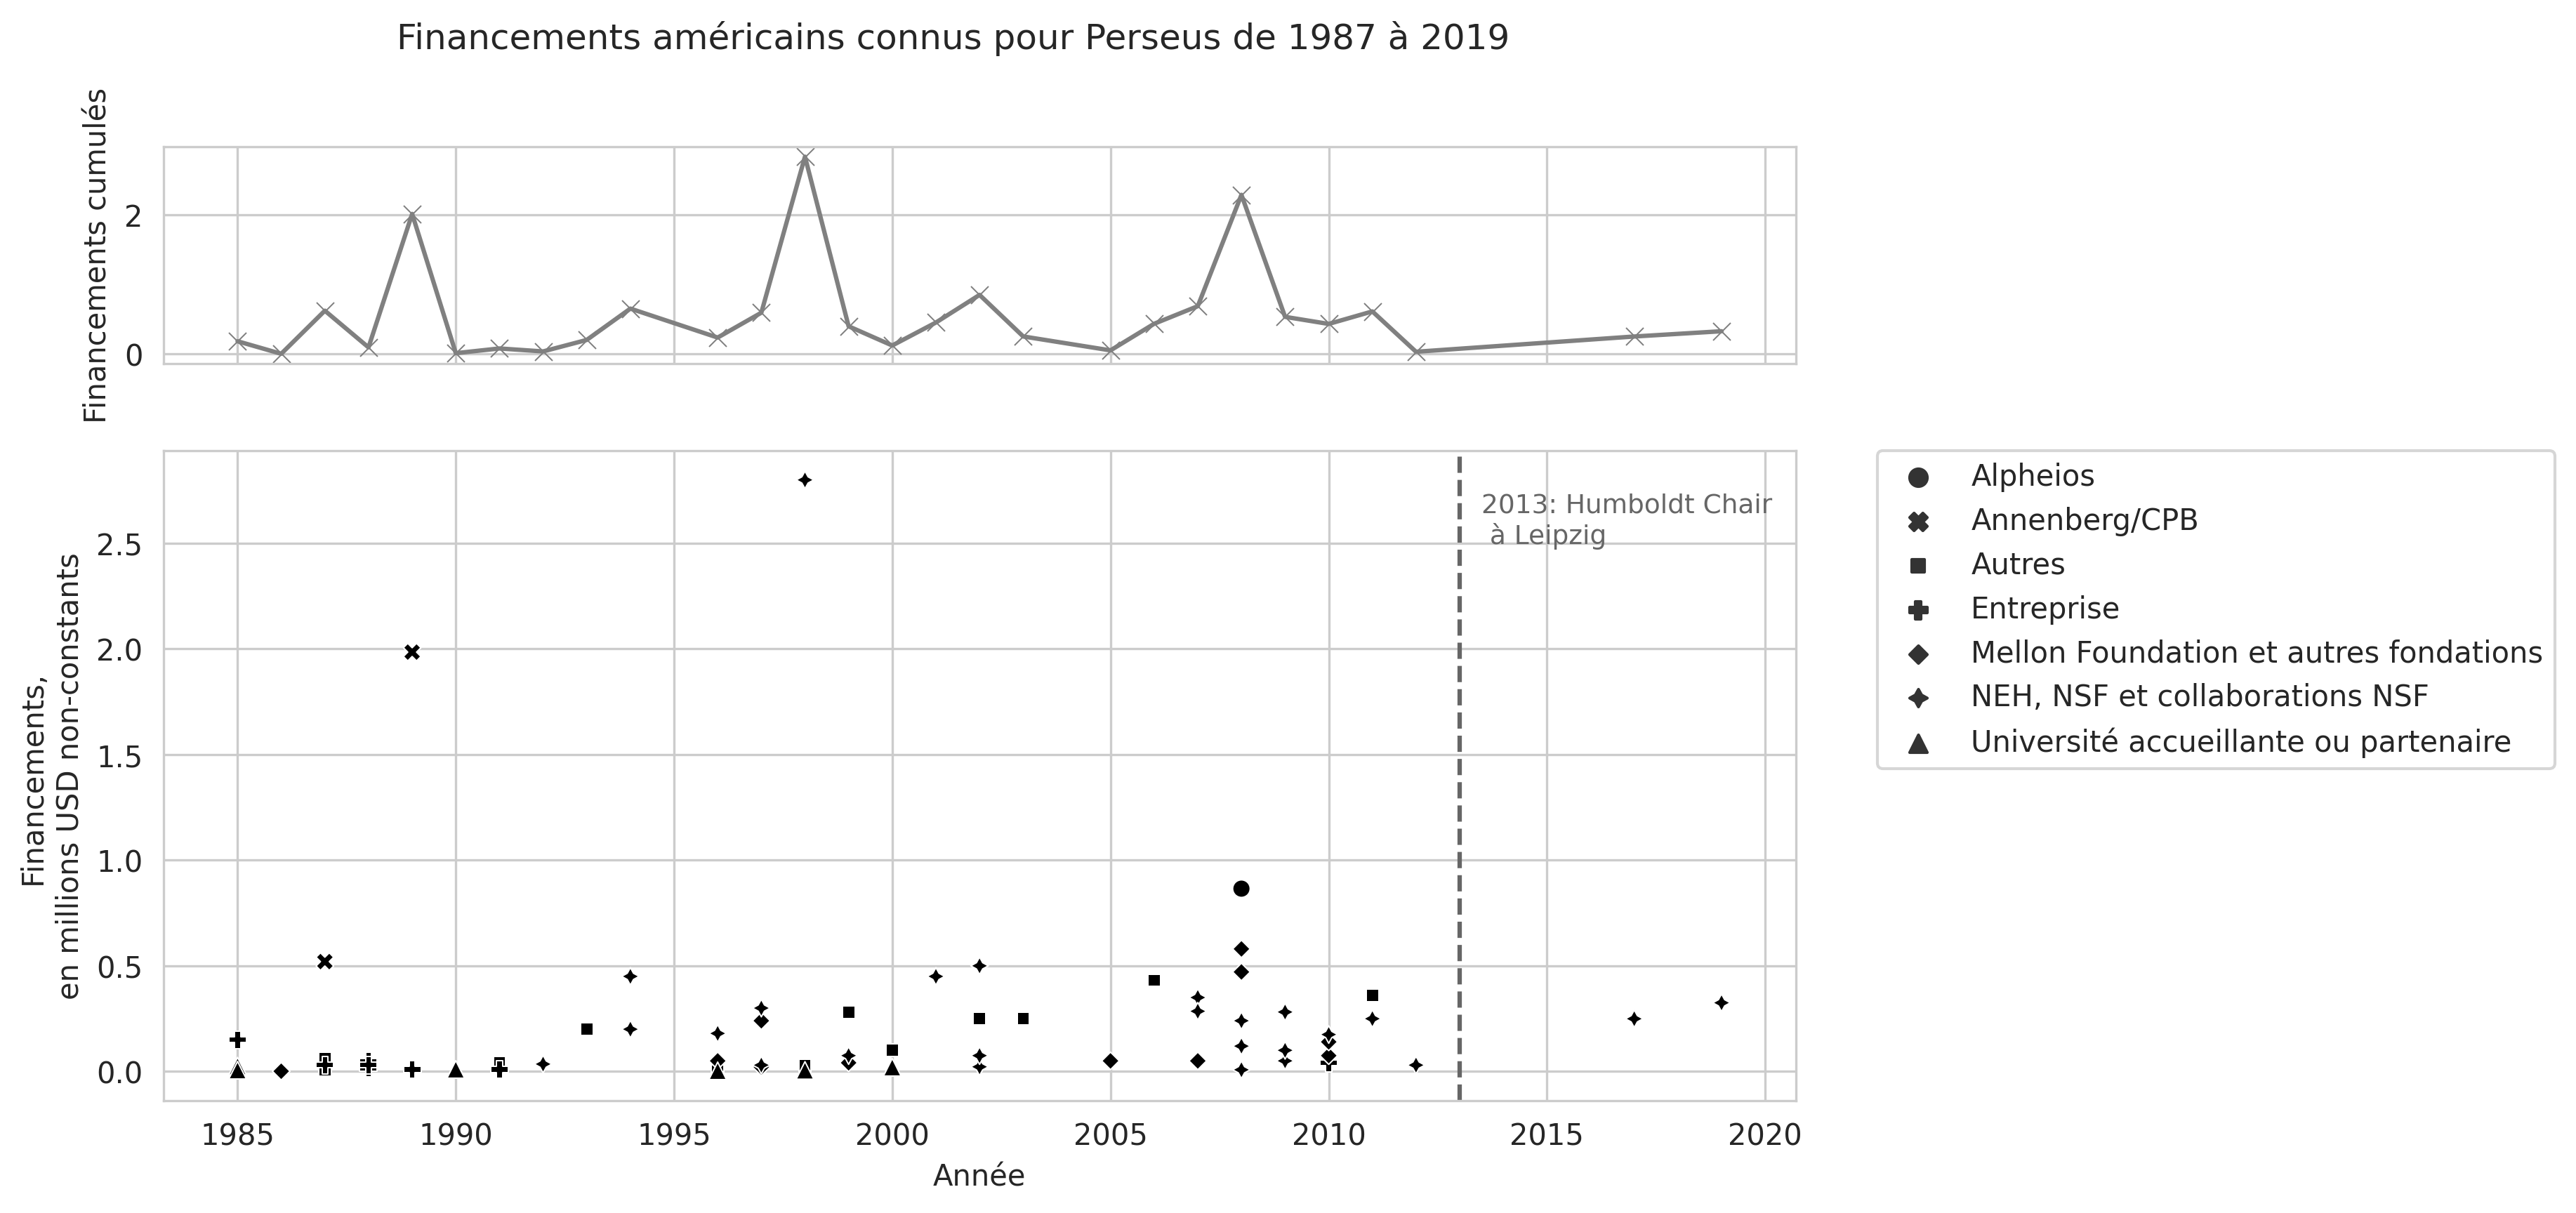
\includegraphics[width=\linewidth]{figures/chap1/part1/PerseusFinancements.png}
    \caption{Financements américains connus de Perseus, en millions de dollars non constants, d'après les pages \textit{Grants} de Perseus, le CV de G.~Crane et les archives de la Mellon Foundation et de la NEH. On distingue clairement trois vagues (1: fondation, 2: web, 3: expansion) et l'exportation de Perseus vers l'Allemagne pendant quelques années pour un retour après la fin des financements à partir de 2017.}
    \label{fig:chap1:perseus_fundings}
\end{figure}

Au milieu de la décennie 2000, la fin du financement \textit{A Digital Library for the Humanities} et un ensemble d'autres financements permettent la sortie d'une nouvelle version majeure\footcite{noauthor_gregory_nodate}, la 4.0. La 3.0 ayant subi de nombreuses modifications suite aux besoins émergents de l'ensemble des financements de la seconde phase, son code n'est plus maintenable. La 4.0 est une remise à plat complète du projet Perseus avec un passage vers le langage Java pour le fonctionnement du site, le passage au XML \acrshort{tei} P4 pour ses ressources textuelles et la mise à disposition pour la première fois de ces dernières en téléchargement libre. Ce changement structurel du \textit{backend} s'opère en 2005, suivi d'une mise sous licence \textit{Creative Commons} de ses sources en 2006 et de son code en \textit{open-source} en 2007\footcite{rockwell_face_2013}. Cette troisième phase marquée par la 4.0 voit l'expansion de Perseus dans le domaine textuel se confirmer: à partir de 2000, aucun financement ne concerne la partie archéologique ou visuelle de Perseus, tandis que se développent une bibliothèque sur la guerre civile (2003), une extension pour les textes arabes (2006), le traitement des entités nommées (2007) ou de la grammaire grecque par \textit{treebank} (2008), etc. Les corpus ont grossi, toujours dans un objectif de mise à disposition des traductions\footnote{Avec comme seule source notre expérience pour le projet Perseus, des statistiques de 500~000 visites sur le site par semaine nous sont parvenues.}. En 2013, alors que G.~R.~Crane obtient la ``chaire Humboldt pour les Humanités Numériques'' à Leipzig, la troisième phase s'éteint, et peu de financements sont obtenus du côté américain, malgré une attache conservée à Tufts.

Un phénomène nouveau accompagne cette apparition du web dans les foyers et bibliothèques: la naissance de corpus produits par des non-spécialistes, transformation numérique de ce que l'érudition locale et les sociétés savantes produisaient et produise en papier, avec la mise à disposition par l'effort de particuliers hors du monde académique de documents, données ou analyses scientifiques. Trois corpus existants encore en 2021 naissent sur la période 1995-1998: \textit{Curculio}\footcite{hendry_curculio_1995}, \textit{LacusCurtius}\footcite{lomarcan_lacuscurtius_1999} et \textit{The Latin Library}\footcite{carey_latin_1998} (1998). Les trois se concentrent en particulier sur la problématique des textes latins, et pour cause, ni Perseus ni \acrshort{phi} ne fournissent alors ces corpus. Ils sont rejoints par des projets francophones dans la décennie 2000, qui correspond à l'explosion de l'accès au web en France et en Europe: \textit{Remacle.org} arrive en 2003\footcite{philippe_remacle_site_2008}, \textit{Latin, Grec, Juxta} de Gérard Gréco en 2006\footcite{gerard_greco_latin_2006}. La particularité des sites francophones tient en la carrière professionnelle de leurs fondateurs: tous deux sont professeurs de lettres classiques de formation. Quelle que soit la situation professionnelle de ces créateurs de contenu, ils partagent tous la particularité de réaliser ces projets sans financement propre, en dehors des cadres universitaires, avec parfois une exhaustivité particulièrement importante, comme pour \textit{The Latin Library}, et avec une véritable focalisation sur le latin.

\subsubsection{Les projets nés sur le web}

La fin des années 1990 et la première décade des années 2000 voient aussi l'émergence de projets nouveaux, cherchant à installer durablement dans le paysage numérique les lettres classiques. Si nous en parlons peu, car nous ne les utiliserons pas dans notre recherche, les premiers à se développer sur le web sont de loin les projets épigraphiques, dont plus d'une vingtaine est déjà répertoriée par Tom Elliott pour le compte de la société américaine d'épigraphie latine et grecque en juillet 1998\footcite{elliott_links_1998}. Mais les projets littéraires s'intéressent aussi à la toile et y naissent.

Le premier mouvement de ces projets nés sur le web est celui de projets qui resteront au niveau du HTML: des sites pour lire des textes, donner accès à ces derniers avant tout. En 1996, par exemple, naît la \textit{Bibliotheca Augustana} d'Ulrich Harsch\footcite{harsch_bibliotheca_nodate}, dont il nous est malheureusement impossible de retrouver le contenu original. En 1998, c'est au tour d'\textit{Itinera Electronica} d'apparaître. Elle est construite autour de deux axes: un ensemble de cours (sur quatre niveaux: acquisition, maîtrise, transmission et approfondissement) et de ressources textuelles dont la mise en ligne ne semble remonter qu'à 2002, d'après les journaux du site\footcite{meurant_itinera_nodate}. La \textit{Roman Law Library} sort en 2001: il est produit par des historiens du droit, hors du domaine des lettres classiques, fruit d'une collaboration internationale, et cherche à couvrir ``depuis les premiers textes de l'époque royale jusqu'aux compilations de la période byzantine''\footcite{lassard_roman_2001}. Les corpus naissent peu à peu aux États-Unis et en Europe, en latin comme pour les autres langues, tant que le catalogue est complexe à construire\footnote{D'autant que le passage du temps fait disparaître ces corpus et le peu de références faites dans les ouvrages ou articles scientifiques n'aident pas à en conserver la trace.}. Les outils de développement web sans apprentissage du code font leur apparition, les compétences intègrent les institutions peu à peu. En 1995 sort \textit{Vermeer Frontpage}, renommé \textit{Microsoft FrontPage} en 1996, qui permet le développement de site web sans compétences avancées en programmation, via une interface graphique. Dès 1997, on voit émerger de guides\footcite{la1997guide} à destination des non-spécialistes des communautés éducatives. Un projet de bibliothèque numérique de ressources slaves fait clairement mention de l'usage de \textit{FrontPage} dans son élaboration\footcite{deyrup1998character} et celle de son corpus, tandis que d'autres, tel le projet \textit{Journeys in Time 1809-1822} à l'université de Macquarie (Australie), rejettent son usage pour la production d'un code ``plus propre''\footcite[p.~41]{10.3316/informit.752609435027594}. Dans la plupart des cas précédemment mentionnés, ils survivent -- c'est ainsi qu'on les connait aujourd'hui -- et se sont enrichis, mais ne sont jamais sortis du contexte des sites web statiques, précompilés en HTML.

La fin 1990 et surtout le début 2000 voient des innovations majeures dans le monde du développement web et de la gestion de corpus électroniques. D'abord, les bases de données SQL (notamment les serveurs MySQL) et le langage PHP voient le jour et dominent rapidement le monde du développement amateur, tout en se faisant parallèlement sa place dans le monde du développement professionnel\footnote{Malgré nos recherches, nous n'avons pas trouvé d'autres sources sur ce sujet que celles que nous citons. Et pourtant, le début des années 2000 voit l'émergence de sites à tutoriel comme celui du \textit{Site du zéro}, la réduction des prix pour l'hébergement de sites, la naissance (et la mort) des salons de discussions pour l'entraide qui favorisent clairement la formation en autodidacte d'une nouvelle génération de développeurs. C'est en tout cas notre expérience de ces années-ci.}. Associé aux serveurs Apache\footcite{smith_lamp_nodate}, facile à mettre en place pour les hébergeurs comme Free en France et d'autres, il devient facilement possible de déployer des sites dynamiques à bases de données relationnelles avec une formation rapide à la programmation. Des outils de publication (\acrlong{cms}) faciles à installer voient le jour et accompagnent ce mouvement technologique\footcite{purer_php_nodate}. Parmi ces applications plus complexes, on notera l'apparition entre autres de \textit{Musisque deoque}\footcite{gelderblom_musisque_2008}. Dans son compte-rendu, Werner Gelderblom indique qu'il s'agirait du premier corpus -- il parle d'archive -- à intégrer les variantes et l'apparat critique\footnote{``\textit{The important innovation of MQDQ is that it is the first large-scale archive to include [apparatus] for a growing number of texts, and that it also provides effective search tools for them}'', \cite[p.233]{gelderblom_musisque_2008}}. D'autres projets similaires se développent: ils sont fondés sur des bases complexes, avec des technologies \enquote{avancées} comparativement à du pur HTML, comme le CGL\footcite{garcea_corpus_2010}. Ce dernier montre par ailleurs l'inconvénient de cette nouvelle couche de complexité: si \textit{MQDQ} est encore en ligne aujourd'hui, le \textit{Corpus Grammaticorum Latinorum} a complètement disparu\footnote{Une nouvelle version est prévue depuis quelques années.}; l'hébergement de simples fichiers HTML et celui d'applications complexes et dynamiques ne posent pas les mêmes défis.

Les années 2000 sont aussi celles de l'adoption par les \textit{guidelines} TEI du XML, d'abord avec la TEI P4 en 2001, puis avec la TEI P5 en 2007. La technologie prend de plus en plus de place dans plusieurs champ universitaires, la liste des participants au meeting de 2003 montre par exemple cette belle diversité de domaines\footnote{\url{https://tei-c.org/Vault/MembersMeetings/2003-info/mm22.html}}. En 2007, une étape supplémentaire est passée: la portée de la réunion annuelle de la TEI change de forme, passant du nom \textit{annual members meeting} à celui d'\textit{annual conference}, on ne publie plus la liste des participants à cette réunion, laissant penser qu'elle est de toute façon trop lourde pour être publiée\footcite{noauthor_members_nodate}. S'il n'a pas fallu attendre ces changements organisationnels pour que la grammaire TEI soit une promesse attirante, ils en sont autant d'indices de son adoption croissante par une grande variété d'individus et d'institutions. Dès 2001, T.~Nellhaus dresse le portait d'un outil pouvant révolutionner les bibliothèques dans leur mise à disposition de corpus grâce à la standardisation qu'elle implique: pour l'auteur, sa souplesse et sa capacité de représenter des faits précis représentent une opportunité, bien qu'il ne soit pas sans défauts\footcite{nellhaus_xml_2001}. Dès 2002, l'\acrfull{ehess} via le laboratoire en médiévistique  \acrfull{ciham} à Lyon adopte la TEI pour l'édition de sermons et d'autres projets à travers les figures tutélaires de Marjorie Burghart et Nicole Dufournaud\footcite{burghart_edition_2011}. Dès 2002 aussi, l'\acrfull{enc} adopte via sa cellule numérique le standard\footcite{poupeau_les_2006}. Chacune de ces institutions évoque la même raison: la TEI, à travers son encodage fin de phénomènes divers (linguistiques, historiques, littéraires, etc.), est un langage pivot permettant de nombreuses sorties et interprétations dont le HTML de lecture -- reproduisant presque les limites de l'imprimé augmenté des liens hypertextes -- n'est qu'une vue. C'est la même raison qui permet à G.~Crane de crier victoire quelques années plus tôt au sujet du passage de Perseus au web.


Dans le monde des lettres latines antiques, peu de projets adoptent dans un premier temps cette technologie, en dehors de Perseus qui avait parié dessus dès la fin des années 1980.  D'une part, il existe le projet \textit{Hyperdonat}. Il est à notre connaissance la première et seule édition scientifique d'une œuvre latine littéraire classique ou tardive raisonnablement longue\footnote{Il existe quelques extraits ici et là, ou quelques œuvres courtes comme le texte de Calpurnius dont nous parlons plus bas.} à utiliser le média web et des sources TEI\footcite{bureau2008hyperdonat}. L'usage de cette technologie est d'ailleurs justifié par Bruno Bureau comme le seul moyen d'éditer la base de données que représentent les commentaires de Donat, loin de l'édition d'un texte linéaire que serait celui d'un Victor Hugo par exemple\footcite[La comparaison est la nôtre.]{chaire_de_recherche_sur_les_ecritures_numeriques_exemple_2018}. D'autres tentatives existent, mais même des initiatives aussi prometteuses que la \acrfull{ldlt}, cherchant à simplifier et promouvoir l'édition critique de textes en TEI, n'arrive à proposer qu'une seule édition de texte (Calpurnius) après des années de mise en place. Comme le note d'ailleurs le porteur de ce projet, Samuel J.~Huskey, en 2019, ``les vraies éditions critiques sur internet sont encore rares''\footnote{``\textit{truly critical editions on the internet are still rare}'', \cite{huskey_digital_2019}}. De l'autre côté du spectre des projets en TEI, hors des objectifs d'éditions critiques, se trouve aussi le projet italien de la  \textit{Latin Digital Library of Late Antiquity} (DigilibLT)\footnote{\textit{Biblioteca digitale di testi latini tardoantichi}, d'où le LT.} dont l'objectif est de produire un nouveau corpus de textes tardifs, absents de Perseus, sans pour autant en proposer de nouveaux établissements de texte. À partir d'éditions imprimées globalement plus récentes que celles de Perseus, plutôt issues de la période 1950-2000, elle propose une collection cataloguée de textes sur la période du deuxième au huitième siècle, incluant des textes impossibles à trouver ailleurs sous format numérique, comme des traités de médecine et de gynécologie. \textit{DigilibLT}\footcite{lana_metodologie_2012} prend par ailleurs le même chemin que celui du projet \textit{Perseus} en affirmant l'importance du caractère \textit{open access} et libre de son projet, dont le corpus est téléchargeable dès sa fondation\footnote{Dans son article, Maurizio Lana titre une de ses parties ``\textit{Accesso aperto, licenze Creative Commons, software libero}'' (fr. Accès ouvert, licence Creative Commons, logiciel libre). \cite{lana_metodologie_2012}}. Mais le monde de la TEI latine classique et tardive s'arrête là, du moins pour les œuvres ``littéraires'' (on inclut les traités de médecine): l'épigraphie a -- elle -- bien adopté l'usage de la TEI et de sa variante Epidoc\footcite{elliott2007epidoc} pour la publication de ces corpus de textes\footcite{bodard2007inscriptions,cayless2010epigraphy}.

\subsubsection{OCR et corpus de masse}

La littérature classique en accès ouvert commence à être bien couverte: il reste quelques textes impossibles à trouver en format numérique , comme les \textit{Declamatio Minores} de Quintilien ou les auteurs fragmentaires, mais ils restent marginaux. Du côté de la littérature tardive, entre DigilibLT, la \textit{Patrologia Latina} et le CSEL, la couverture tend à être meilleure, même si de nombreux textes ne sont pas édités ou ne sont tout simplement pas encore tombés clairement dans le domaine public\footnote{La question du droit d'auteur sur les éditions de textes anciens est complexe, spécifique à chaque territoire, y compris en Europe, et pose de vrais problèmes d'interprétations, dont certains producteurs de corpus se plaignent, comme Philipp Roelli dans \cite{roelli2014corpus}. Sur le plan national, de nombreuses publications existent, comme \cite{combalbert_lediteur_2015, demonet_confiscation_2018}. Sur le plan international, et celui des textes latins \cite{fischer2017digital, dillen_digital_2016}. Sur des textes plus récents, \cite{dusollier_international_2019}}. Au contraire, les littératures médio-latine et néo-latine sont particulièrement absents des corpus en ligne, et leur mise à disposition tarde. Dans ce contexte, l'idée de recourir à des dépôts massifs de numérisations photographiques émergent pour élaborer de nouveaux outils ou offrir de nouvelles approches des textes.

En 2011 et 2012, David Bamman, avec G.~Crane\footcite{Bamman:2011:MHW:1998076.1998078} puis avec David Smith,\footcite{bamman_extracting_2012} s'intéresse pour la première fois à un corpus en friche: celui des campagnes de numérisation, majoritairement privées dans son cas précis, et du résultat de la reconnaissance optique de caractères (\acrshort{ocr}) appliquées à ces documents. Il dénombre, en 2012, 27~014 textes catalogués comme latins dans l'index du projet \textit{Internet Archive}, comprenant tout autant les classiques latins que les thèses et autres ``commentaires de la philosophie d'Hegel'' produits en Allemagne, mais écrits en latin au dix-neuvième siècle\footcite{bamman_extracting_2012}. Puis, en triant les données, en partie manuellement\footcite{bamman_dbammanlatintexts_2018}, il obtient une liste de plus de onze mille ouvrages comprenant environ 1,38 milliard de mots\footnote{Ce chiffre est à prendre avec une certaine précaution: la méthode de calcul des mots n'est pas précisée et la définition de ce qu'est un mots ici non plus.}. Au moyen des données récupérées, il met à disposition les premiers \textit{embeddings} massifs de l'histoire du latin approché par méthode computationnelle. Cependant, ses données sont problématiques: d'une part, la méthode de vérification manuelle du catalogue n'est pas expliquée; d'autre part, le résultat final contient des documents dont l'\acrshort{ocr} est absolument inexploitable (``\texttt{tkei: SiiimiemfiBgMiffem mvemsfimUttrUffHk rejcijps}'' étant un des exemples de mauvaise transcription qu'il cite lui-même).

\begin{figure}
    \centering
    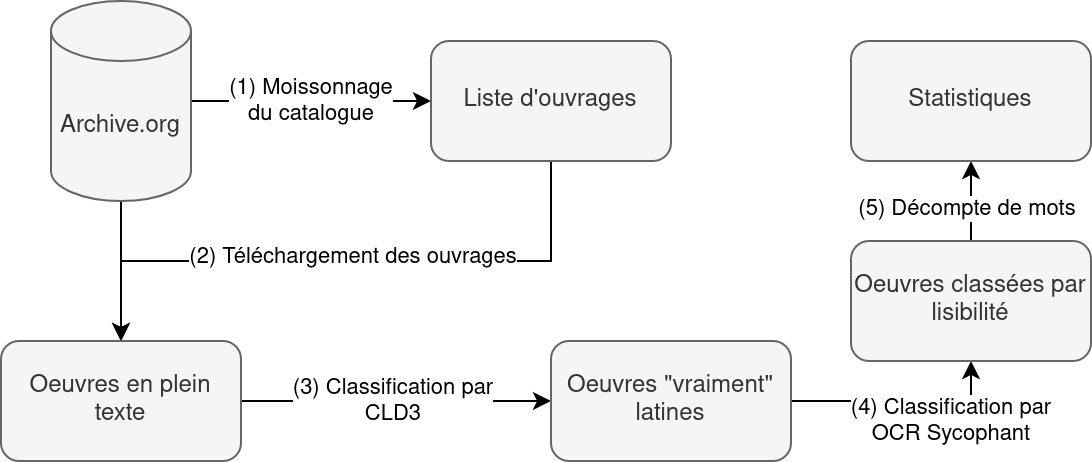
\includegraphics[width=.8\linewidth]{figures/chap1/part1/ocrSycophant.png}
    \caption{Récapitulatif de la chaîne de traitement appliquée sur Archive.org}
    \label{fig:chap1:workflow-sycophant}
\end{figure}

L'OCR ayant progressé depuis 2013, et la méthode de D.~Bamman n'étant pas totalement claire, nous nous sommes intéressé à l'évolution du dépôt \textit{Internet Archive}. Pour faire cela, nous avons traité les données de cette bibliothèque numérique en cinq étapes (reproduites en figure \ref{fig:chap1:workflow-sycophant}). Les œuvres classées comme étant en latin par l'\textit{Internet Archive} sont téléchargées. On sélectionne au hasard un quart des lignes de chacune des œuvres sur lesquelles on applique un classificateur de langue\footcite{salcianu2018compact}. 
% GABAY REPRENDRE ICI 6/01, p. 35
Ce classificateur indique des statistiques pour plusieurs langues s'il a des doutes sur cette classification: on retient alors qu'une ligne est classée comme latine si elle a un score supérieur à 60\% en latin\footnote{Ce seuil a été fixé pour prendre en compte l'existence d'œuvres bilingues.}. Après ce traitement, on applique un outil conçu par nos soins pour classer les lignes transcrites en terme de qualité (compréhensibles ou non), OCR~Sycophant\footcite{Clerice_OCR_Sycophant_2021}. OCR~Sycophant a été développé autour de modèles de classification classiques basés sur des n-grams, et a été entraîné à partir d'un dataset de phrases du corpus Archive.org sélectionnées aléatoirement et annotées à la main: ont été classées comme ``incompréhensibles'' les données qui n'étaient pas en latin (\textit{eg.} ``\texttt{" Mr Bryce's test, on account of the difficulty of pro-}''), qui étaient illisibles (eg. ``\texttt{"7 „ 7- f Ak. —2 vi rt*- ('wbrf-}'') ou difficilement lisibles (\textit{eg.} ``\texttt{(Hciucuto qucfo quob fwutuinlto}''), ou encore qui correspondaient à des lignes considérées comme trop courtes (\textit{eg.} ``\texttt{5}''). Ce classement effectué, on obtient un pourcentage de lignes estimées propres : on compte alors les \enquote{mots} de chaque texte (un mot étant considéré simplement comme un élément séparé par un espace).

Ce résultat donne des chiffres absolument prometteurs, tout en demandant une forme de patience. On compte dans les documents disponibles en latin presque 5~000 œuvres avec une qualité d'OCR à plus de 90\%(\textit{cf.} table \ref{tab:chap1:latin-OCR}) représentant 635 millions de mots. Si l'on ajoute à ce corpus les textes avec plus de 80\% de qualité OCR, on atteint les 1,451 milliard de mots et un peu plus de 17~000 ouvrages. Il existe probablement des doublons parmi les textes, mais un corpus de taille inégalée, en quantité et en diversité, existe dans ces dépôts: avec ces deux catégories de textes propres, on atteint près de dix fois plus de mots que les œuvres contenues dans \textit{Corpus Corporum}, et en ne prenant en compte que la bibliothèque \textit{Internet Archive}.

\begin{table}[ht]
\centering
\begin{tabular}{l|rrr}
\toprule
                               & Nombre de volumes & \% du total & Nombre de mots \\ \midrule
Qualité \textgreater 90\% OCR  & 4 946              & 23.73       & 635 201 534    \\
Qualité \textgreater 80\% OCR  & 12 169             & 58.38       & 816 236 079      \\
Qualité \textgreater 60 \% OCR & 3 709              & 17.79       & 182 697 928      \\
Reste                          & 19                 & 0.09        & N/A           \\ \bottomrule
\end{tabular}
\caption{Statistiques sur les ouvrages latins disponibles sur Archive.org au début juillet 2021}
\label{tab:chap1:latin-OCR}
\end{table}

La question de l'OCR et de sa qualité (surtout pour les œuvres imprimées avant la fin du dix-neuvième siècle), deviennent donc prépondérantes dans le contexte de l'acquisition de textes fac-similaires (et donc non édités). Le problème de la reconnaissance de texte pour les œuvres des incunables et de l'époque moderne, avec ses S longs et ses restes d'abréviations, est peu à peu réglé par la mise à disposition massive de données d'entraînements et de modèles adaptés. Dans ce cadre, le travail de Simon Gabay autour des imprimés du 17e siècle est absolument majeur et fondateur\footcite{simon_gabay_2020_3826894}: son usage a permis de générer de très bons modèles OCR\footcite{gabay:hal-02577236} et, à partir de quelques données latines\footcite{Clerice_CREMMA_16_18_Prints_2021}, permet de produire des données propres de textes latins imprimés avant le 19e siècle, de l'\textit{Utopie} de Thomas More à des œuvres en zoologie du 18e siècle en passant par l'\textit{Historia de duobus amantibus Euralio et Lucretia}, avec des taux de reconnaissance à plus de 96\%. 

Mais un autre enjeu pour la mise à disposition de texte arrive aussi à travers la Reconnaissance d'Écriture Manuscrite (REM, ou plus communément l'anglais HTR pour \textit{Handwritten Text Recognition}). La transcription automatique des documents de la pratique et des manuscrits littéraires, quel que soit leur genre, apportera une autre masse de données pour l'étude du latin sur le temps long. Le développement de cette technologie, sa popularisation par Transkribus\footcite{kahle2017transkribus}, sa mise à disposition \textit{open source} par Ben Kiessling via Kraken\footcite{kiessling2019kraken} puis eScriptorium\footcite{kiessling_escripto}, ont permis l'émergence de modèles partagés extrêmement performants. Les travaux d'Ariane Pinche sur les manuscrits en ancien français\footcite{Pinche_CREMMA_Medieval_an_2021} avec une reconnaissance des caractères supérieur à 95\% ou les travaux de Dominique Stutzmann\footcite{hazem2020books} ont montré que cette approche était prometteuse et pouvait potentiellement passer à l'échelle. Il est probable que l'étude quantitative du latin soit largement redéfinie par la mise à disposition de ces corpus nouveaux sur le moyen terme, en s'attaquant de front aux dépôts institutionnels nationaux ou régionaux, comme la Bibliothèque nationale de France et son dépôt Gallica. Dans ce cadre, des projets comme le Gallicorpora, dont font d'ailleurs partie S.~Gabay et A.~Pinche, montreront rapidement ce à quoi l'on peut s'attendre sur le court terme, avec le développement d'une chaîne de traitement pour la production de documents fac-similaires encodés finement en TEI.

Si l'approche évoquée précédemment est celle d'une approche massive, bruitée et sans réelle intervention humaine, une approche qualitative des corpus en friche est aussi possible. La révolution de la qualité des données obtenues via OCR a permis aussi de développer de nouveaux projets, comme VELUM dirigé entre autres par Bruno Bon pour la mise en place d'un corpus médiéval latin de texte OCRisés\footcite{bon2019challenges}. Du côté des périodes classiques et tardives, il faut alors se tourner vers l'initiative \acrfull{ogl} menée par G.~Crane d'abord depuis l'université de Leipzig puis de Tufts.

Né entre 2008 et 2009, \acrshort{ogl} est le fruit d'un besoin ressenti par deux enseignants et chercheurs en lettres classiques associés au \acrfull{chs} (\acrshort{chs}) d'Harvard\footnote{Les locaux de ce dernier sont par ailleurs complètement distincts de ceux d'Harvard, au point d'être dans deux États et deux villes différentes: Cambridge, Massachusetts et Washington DC}: Neels Smith et Christopher Blackwell\footcite{muellner2019free}. Ce projet a pour objectif de produire un corpus pour le grec intégralement \textit{open source}, gratuit et accessible, et standardisé afin de pouvoir s'assurer de la collaboration et de la réutilisation par des partenaires divers. Une première tentative de partenariat avec le TLG échoue en 2010, et pousse l'OGL se lancer dans la compilation d'un nouveau jeu de données, qui ne prendra forme qu'en 2015.

Neel Smith est un proche ami de Gregory Crane: ils ont partagé les bancs de Harvard, ont travaillé en équipe sur HCCP et les premières moutures de Perseus et ont partagé le même directeur de thèse, Gregory Nagy, directeur depuis 2000 du CHS. En 2013, Gregory Crane obtient donc la \textit{Digital Humanities Chair} à l'université de Leipzig, où il a pour objectif de relancer le projet Perseus. Dans ce cadre, ses premières décisions sont simples: il faut agrandir le corpus gréco-latin, en particulier sur le premier millénaire de notre ère, et ajouter un grand nombre de traductions. Les pères de l'Église et l'ensemble de la littérature tardive sont, au moment de ce choix, indisponibles en accès libre. Pour le latin, l'OCR a fait les progrès qui permettent à l'équipe de Perseus de mettre en place de nouveaux corpus, dont les deux premiers sont le \textit{\acrfull{csel}}\footcite{noauthor_csel_nodate} et la \textit{\acrfull{pl}} de Migne. Si la \acrshort{pl} a été introduite précédemment et existait dans des versions concurrentes, le CSEL est quant à lui un corpus d'éditions critiques des pères latins de l'Église. Née en 1864, cette initiative autrichienne de 1864 toujours en cours et hébergée à l'université de Salzburg\footcite{noauthor_history_nodate} a publié depuis sa fondation plus d'une centaine de volumes comprenant potentiellement plusieurs œuvres, comme le volume 10 constitué des œuvres complètes de Sidulius (IXe siècle), et dont une partie est tombée, avec son apparat critique, dans le domaine public.

Au niveau technique, ces corpus sont transcrits automatiquement, puis corrigés et structurés en XML TEI par des entreprises spécialisées, dont l'entreprise française Jouve et sa succursale malgache. Leur XML est ensuite adapté aux attentes de Perseus par des équipes internes puis mis à disposition sur Github. C'est ce même fonctionnement qui est repris lors de la mise en place de l'alliance entre le CHS, l'université de Mount Alison et les équipes de G.~Crane. Dans l'article de L.~Muellner, on apprend que l'OCR est réalisée par les équipes de Mount Alison, sous l'égide de Bruce Robertson qui entretient des modèles pour l'OCR grecque. Les données sont envoyées ensuite à l'entreprise plurinationale \textit{Digital Divide Data} (DDD; Cambodge, Kenya, Indonésie) pour leur mise en Epidoc, grammaire XML retenue par Perseus. Le coût budgété de numérisation et d'encodage par DDD est de 50~000\$ pour quatre millions de mots, soit bien moins que les premiers projets des années 1970 et 1980. Enfin, la mise en conformité et la vérification des données sont finalement assurées par des stagiaires, étudiants de la licence au doctorat, hébergés d'abord uniquement par le CHS puis par l'université de Virginie\footcite{robertson2019optical}.

La production de l'ensemble de ces corpus a permis à Perseus de se tourner vers une nouvelle version, en partie financée par le CHS, Perseus 5\footnote{\url{https://scaife.perseus.org/}}, dont la mise à jour est automatiquement liée à l'évolution des corpus, contrairement à la version 4, et qui a été l'objet d'une refonte totale de l'infrastructure de Perseus. Cette version a abandonné -- pour le moment -- les données graphiques (archéologiques, histoire de l'art, etc.) pour ne s'intéresser qu'aux données textuelles.

Enfin, avec l'apparition de tous ces projets se pose la question de l'éclatement des corpus sur internet. Entre les données de Perseus, de DigilibLT, d'autres projets comme le \textit{Corpus Grammaticorum Latinorum} de Jussieu (CGL), l'accès à un corpus latin unifié devient problématique. C'est un problème d'autant plus important que ces sites ne partagent pas une architecture commune qui pourrait permettre de centraliser les recherches sur de multiples corpus. En 2011, Philipp Roelli, un éditeur de texte aussi intéressé par la linguistique de corpus, met en route le projet \textit{Corpus Corporum} à l'université de Zurich\footcite{roelli2014corpus}. Ce projet est très peu financé en dehors d'une aide de la chaire de latin et d'une partie des fonds de la COST-Action IS1005 dont l'objectif principal était la formalisation d'un réseau de recherche autour du latin médiéval\footnote{\textit{Corpus Corporum} est donc plus une externalité positive de cette dernière que l'un de ses objectifs.}. Ph.~Roelli le définit comme une ``meta-collection'': \textit{Corpus Corporum} ne produit pas de numérisation ou d'édition numérique, il centralise, en harmonisant, les données d'une dizaine (en 2014) puis d'une trentaine d'autres projets (en 2021), accumulant ainsi en un seul lieu presque 164 millions de mots à la fin 2021 représentant toutes les périodes du latin, du classique au néo-latin. Bien que techniquement ``rustique'' du côté client\footnote{L'usage des \textit{iframes} a presque complètement disparu du web, hormis sur \textit{Corpus Corporum}.}, le projet a l'avantage d'être rapide, facile d'usage -- à l'image de \textit{The Latin Library} -- et de permettre l'accès à des corpus perdus comme les CGL, indisponibles sur leur site d'origine depuis quelques années.

Après l'avènement du micro-ordinateur et du web, les corpus latins ont ainsi évolué pour atteindre aujourd'hui une ouverture sans commune mesure. Pour les plus grands classiques, il est possible d'en trouver des éditions voire des traductions -- en anglais majoritairement -- assez facilement en plein texte. Et quand cela n'est pas possible, on peut toujours faire recours aux dépôts institutionnels ou privés tels qu'Archive.org ou HathiTrust aux États-Unis afin d'obtenir la numérisation d'un de ces ouvrages. Cette révolution, sur presque cinquante ans, est celle de l'accès aux textes latins classiques et tardifs dans leur intégralité -- ou presque -- et de manière gratuite, permettant ainsi de produire de nouveaux questionnements et de développer de nouvelles approches.

\section{Constitution d'un corpus de sources littéraires latines}

Après cinquante ans de compilations et de production de textes numériques, le nombre de corpus disponibles -- qu'il soient ouverts, fermés ou à réutilisation limitée -- est assez important pour permettre une recherche plein texte ou la production d'exempliers numériques. Le travail de Ph.~Roelli montre que, en produisant des corpus ouverts et ré-exploitables, les projets comme \textit{Perseus} et \textit{DigilibLT} ont constitué des gisements de textes analysables, indexables et réutilisables dans un contexte autre que celui d'une lecture linéaire et ``manuelle''. Pour notre recherche, nous aurons besoin d'un corpus permettant d'effectuer des recherches plein texte, d'extraire des exemples. Beaucoup d'options s'offrent à nous pour constituer ce nouveau meta-corpus, de l'utilisation d'outils commerciaux comme la \acrshort{llt} à celle de corpus en friche de l'\textit{Internet Archive}. C'est pourquoi il semble primordial de construire notre méta-corpus autour de principes, que l'on appelle généralement \enquote{bonnes pratiques} ou éthique, guidant ensuite la compilation ou réutilisation d'un tel corpus. 

Nous décrirons dans un premier temps ces principes et ce qui les rend indissociables de la création de corpus. Dans un second temps, nous présenterons les choix techniques, la méthode de compilation du meta-corpus et le résultat de cette dernière. Enfin, nous étudierons l'impact que peut avoir l'un des choix techniques effectué, à savoir le choix d'avoir un corpus plus petit mais dont la structure de citation est \textit{machine actionable}.

% ToDo: A RÉÉCRIRE car le plan à changer
N% ous étudierons ensuite l'importance de l'encodage fin de textes et de l'impact que son manque peut avoir sur la production de savoir via des analyses statistiques. Enfin, nous discuterons de la compilation du corpus effectuée à partir de l'œuvre scientifique de J.~N.~Adams, des limites de cette dernière, mais aussi des méthodes employées pour compiler cette collection.

\subsection{Objectifs et prérequis d'un corpus pour une analyse automatisée}

\begin{quote}{J.-B.~Camps}
\enquote{La distinction entre humanités « numériques » et « computationnelles » est dans l’air. Au‑delà d’un pur choix terminologique distinctif ou d’un retour aux \textit{humanities computing} du XXe siècle, la revendication d’une dimension computationnelle rend compte d’un basculement, à mon sens éminemment souhaitable, d’une perspective tournée vers la diffusion et la publication électronique, à un accent mis sur les données et leur exploitation pour la création de nouveaux savoirs scientifiques.}\footnotemark
\end{quote}
\footnotetext{\textcite{camps_ou_2018}}

Le constat de Jean-Baptiste Camps est juste: depuis les années 2000 et 2010 en particulier, la technicisation de l'analyse des documents et des sources, à travers l'explosion de l'usage de la stylométrie par exemple, et le besoin d'une reconnaissance à part de cette technicisation a donné lieu à de nouvelles sous-communautés des humanités numériques, avec leurs réseaux parallèles de conférences. En juillet 2019, à la suite de la conférence annuelle de l'\acrfull{adho}, association internationale principale des humanités numériques\footnote{Cette association, l'\acrshort{adho}, organise à ce moment-là DH2019 à Utrecht.}, un groupe d'intervenants décide à remédier à cette frustration. Quelques semaines plus tard, un sondage est publié, et son phrasé d'introduction est clairement revendicatif: \enquote{Malgré l'essor indéniable de ce nouveau domaine de recherche [les humanités computationnelles], de nombreux chercheurs estiment qu'il n'existe pas d'endroit approprié, axé sur la recherche, pour présenter et publier leurs travaux informatiques sans perdre de vue les questions relatives aux sciences humaines\footnote{\enquote{\textit{And yet, despite the undeniable growth of this new research area, many scholars still feel that there is no suitable research-oriented venue to present and publish their computational work that does not lose sight of questions relevant to the humanities.}}\textcite{noauthor_computational_nodate}}.}. Suite à cet appel de ce qui s'appelle alors la CoHuRe (Computational Humanities Research, plus tard CHR), on voit l'émergence de \enquote{contre conférences DH} avec la CHR 2020 puis 2021, ou encore des événements encore plus spécialisés comme NLP4DH\footcite{noauthor_workshop_nodate}. Si la reconnaissance du travail d'analyse technique est importante, nous différons sur l'apparente exclusion mutuelle qu'opèrerait ce \enquote{nouveau} paradigme de la recherche numérique. Dans un champ éminément protéiforme comme les humanités numériques, que l'on peut définir comme une \enquote{science auxiliaire des sciences humaines}\footnote{À l'image des \enquote{sciences auxiliaires de l'histoire}, que sont par exemple la paléographie et la numismatique.}, il faut trouver un équilibre, un balancement, plus qu'un \enquote{basculement}, entre le travail de génération de données, fruits d'un travail de recherche, et celui d'analyses. La production de corpus, de la collecte de textes\footnote{Ou d'autres types de données: ce constat est le même pour les annotations linguistiques par exemple.} pré-existant à leur édition en passant par leur contrôle qualité, est une mission qu'il ne faut pas négliger dans une approche plus ``computationnelle'' des sciences humaines, sans quoi les humanités computationnelles ne sont plus des humanités, mais de l'informatique appliquée.

\subsubsection{Le choix d’un corpus \textit{open source}: traçabilité des textes et reproductibilité}

Sans redéfinir ce qu'est un corpus, il est intéressant de s'arrêter un temps sur les définitions des deux dictionnaires français les plus populaires, \textit{Le Robert} et le \textit{Larousse}\footnote{Version en ligne de décembre 2021.}, pour questionner les traits qui caractérisent notre objet. \textit{Le Robert} définit le corpus comme un ``Ensemble fini de textes choisis comme base d'une étude.'' tandis que le \textit{Larousse} prend -- par un heureux hasard -- l'exemple des corpus grecs pour appuyer sa première définition: ``Recueil de documents relatifs à une discipline, réunis en vue de leur conservation : Corpus des inscriptions grecques.'' et rejoint légèrement le \textit{Robert} pour sa seconde (``Ensemble fini d'énoncés écrits ou enregistrés, constitué en vue de leur analyse linguistique.''). Si les deux dictionnaires se rejoignent sur un point --  à savoir, le corpus est une collection de documents, potentiellement de textes --, ils évoquent deux finalités différentes. 

La première, la conservation -- sous-entendue la maintenabilité et l'accessibilité en un même endroit, physique ou numérique, d'un ensemble documentaire -- n'est mentionnée que par le \textit{Larousse}. Dans son article de 2013, Alex H.~Poole fait le constat que ``les humanités numériques pivotent autour des données''\footnote{``\textit{The digital humanities pivot around data.}''\cite{poole_now_2013}} mais aussi que ces dernières, au format numérique, sont ``notoirement fragiles, d'une courte espérance de vie, et facile à manipuler sans laisser forcément de traces, rendant la fraude difficile à détecter [..., sachant que] la plupart des données collectées ne sont ni organisées ni publiées''\footnote{``\textit{Our Cultural Commonwealth} report characterized digital data as “notoriously fragile, short-lived, and easy to manipulate without leaving obvious evidence of fraud”. Worse, much collected data were neither curated nor published whatsoever;'', \cite{poole_now_2013} citant \cite{unsworth2006our}}. Nous partageons ce constat -- la capacité de conservation d'un corpus doit être intrinsèque à ces derniers -- et établissons ce point comme premier objectif autour de notre corpus. 

La seconde finalité évoquée est celle de l'analyse (``la base d'une étude'', ``en vue d'une analyse linguistique''). Si nous estimons que cette finalité peut être déplacée (le corpus peut être compilé pour qu'une tierce personne s'en empare), elle est bien évidemment centrale dans notre projet. Et elle demande ainsi de définir l'objectif de notre corpus, car celui-ci définira la forme, l'outillage et les informations nécessaires à y retrouver. Nous reviendrons plus tard sur l'impact qu'a cette finalité sur le corpus, dans son annotation et sa documentation (\textit{cf.} \ref{chap1:method-annotation}).

Il faut cependant ajouter à la notion de corpus développer plus haut d'autres caractéristiques, dont celles de son ouverture, en droit et en accès. A.~H.~Poole la mentionne partiellement dans la citation avec la question de la ``fraude'', mais la position de Borgman\footcite{borgman2012conundrum}, reprise par J.-B.~Camps\footcite{camps_ou_2018}, est à notre sens assez complète. D'après elle, un corpus doit être ouvert pour
\begin{enumerate}
    \item reproduire ou vérifier la recherche,
    \item rendre les résultats d'une recherche publique disponible pour le public,
    \item permettre à d'autres de poser de nouvelles questions aux données
    \item avancer l'état de la recherche et de l'innovation.\footnote{``(1) to reproduce or to verify research, (2) to make results of publicly funded research available to the public, (3) to enable others to ask new questions of extant data, and (4) to advance the state of research and innovation.''\footnote{\cite{borgman2012conundrum} chez \cite{camps_ou_2018}}.}
\end{enumerate}

La question de la reproductibilité, par l'ouverture du corpus et sa documentation, est centrale pour Borgman, Poole et Camps. Si la traçabilité des sources n'est pas une nouveauté pour les lettres et l'histoire -- la citation de ces dernières est extrêmement codifiée afin d'être compréhensible et exhaustive, la transcription des sources de la pratique est souhaitée pour les publications scientifiques --, la reproductibilité des expériences est définitivement nouvelle. D'abord, la notion de recherche expérimentale en lettres comme en histoire est globalement nouvelle, bien qu'elle ne le soit pas nécessairement partout dans les sciences humaines. Ensuite, car la notion de reproductibilité est tout autant complexe dans le monde des sciences dites dures. Comme le dit J.-B.~Camps, ``au fur et à mesure que l’analyse de données prend de l’importance dans la constitution de nouveaux savoirs, le besoin se fait plus criant de vérifier l’intégrité des données, de reproduire les expériences, de vérifier ou infirmer les énoncés qui en découlent.''\footcite{camps_ou_2018}. L'arrivée de ces questionnements scientifiques et la "crise de la reproductibilité" en 2000, que mentionne J.-B.~Camps est suivi peu à peu par une crise en intelligence artificielle\footcite{hutson2018artificial}, traitement automatique des langues\footcite{belz2021systematic} et en histoire computationnelle\footcite{eijnatten_big_2013}.

L'ouverture des corpus rend aussi possible leur analyse et l'analyse de leurs biais, permettant d'aller plus loin que la simple reproductibilité des expériences effectuées. En accumulant des données dont on essaie de tirer des analyses ou même simplement des faisceaux d'indices, la possibilité d'introduire, inconsciemment, des biais de corpus\footnote{Un biais de corpus correspond à toute particularité du corpus liée à sa constitution qui privilégierait une période, un genre, un auteur, etc. \textit{Cf.} en archéologie la définition des biais de corpus, répartis en biais géographiques et méthodologiques, d'Aline Resch\textcite[p.~144]{resch:tel-03218240}} et -- à travers eux -- d'établir des conclusions invalides est un danger éminemment connecté aux corpus fermés. Les conséquences peuvent être importantes dans le domaine de l'intelligence artificielle, le \textit{machine learning} ne pouvant qu'apprendre ce qu'on lui montre. L'exemple le plus connu des dernières années est celui de la reconnaissance d'image de Google, qui, en 2019, avait tout simplement catégorisé des personnes afro-américaines comme gorilles, probablement suite à un problème de données d'entraînement\footcite{lohr2018facial, chokshi2019facial}. Si les conséquences pour notre corpus ne pouvaient être aussi graves et socialement problématiques, il reste que la question du biais est à prendre en compte. Il ne s'agit pas de promettre l'exhaustivité ni la représentativité de ce qui existe ou a existé: le domaine des lettres classiques a depuis longtemps admis la partialité -- dans les deux sens -- de ses sources ainsi que les pertes de nombreuses autres sources. Sur ce sujet, nous reprendrons l'exemple de l'article de I.~D.~Raji \textit{et al.}\footcite{raji2021ai}:

\begin{quote}{\textcite{raji2021ai}}
    \enquote{Dans le livre d'histoires pour enfants \textit{Sesame Street}, ``Grover and the Everything in the Whole Wide World Museum''[Stiles et Wilcox, 1974], le monstre \textit{Muppet Grover} visite un musée qui prétend présenter "tout ce qui existe dans le monde entier". Des exemples d'objets représentant certaines catégories remplissent chaque pièce. Plusieurs catégories sont arbitraires et subjectives, notamment les salles d'exposition des "choses que l'on trouve sur un mur" et de "la salle des choses qui peuvent vous chatouiller". Certaines sont étrangement spécifiques, comme "La salle des carottes", tandis que d'autres sont inutilement vagues comme "La grande salle". Alors qu'il pense avoir vu tout ce qu'il y a, Grover arrive à une porte intitulée "Tout le reste". Il ouvre la porte et se retrouve dans le monde extérieur.\footnote{\textit{``In the 1974 Sesame Street children’s storybook Grover and the Everything in the Whole Wide World Museum [Stiles and Wilcox, 1974], the Muppet monster Grover visits a museum claiming to showcase “everything in the whole wide world”. Example objects representing certain categories fill each room. Several categories are arbitrary and subjective, including showrooms for “Things You Find On a Wall” and “The Things that Can Tickle You Room”. Some are oddly specific, such as “The Carrot Room”, while others unhelpfully vague like “The Tall Hall”. When he thinks that he has seen all that is there, Grover comes to a door that is labeled “Everything Else”. He opens the door, only to find himself in the outside world.''}}}
\end{quote}

Tout comme l'idée d'un musée du monde entier est absurde, l'absence de biais dans un corpus l'est tout autant. Mais la possibilité de les décrire et de les vérifier à travers un corpus ouvert est primordiale pour la critique des résultats.

Nous ajouterons cependant une dernière possibilité derrière l'ouverture de ces données, particulière à leur dimension numérique: l'\textit{open access} et l'\textit{open source} dans ce contexte permettent aussi la croissance et la modification des données sur le long terme, ne figeant pas le corpus à un instant T (bien qu'il soit important de pouvoir revenir à ce dernier pour la reproductibilité). Le corpus de notre recherche doit non seulement survivre à sa publication, mais aussi être corrigé et amendé: il serait probablement présomptueux de le croire exhaustif, sans erreurs, et d'autres seront -- nous l'espérons -- intéressés par son amélioration ou son extension à d'autres textes, d'autres périodes.

Enfin, le corpus doit être \textit{sourçable}, \textit{traçable}. La premier argument à soutenir cet objectif est celui de la \textit{vérifiabilité} et de la possibilité de recompiler ce même corpus au besoin, pour les mêmes raisons qui nous poussent à citer toute bibliographie de manière détaillée et systématique. Ensuite, l'histoire des corpus latin a montré une forte tendance pour le champ à ignorer le travail de production que ces projets ont réalisé, produisant un silence important, à même d'endommager les carrières de nombreux chercheurs et chercheuses. Enfin, cette traçabilité, en plus de respecter l'autorité derrière les numérisations ou les établissements du texte, documente le moment de vie auquel ces textes ont été intégré à notre corpus, y compris avec leurs fautes, leurs manques.

\subsubsection{Un corpus \textit{machine actionable} ?}
\label{chap1:method-annotation}

% De la question de traçabilité découle la question  Capitains
% Citabilité, manipulabilité, compatibilité: XML-TEI et Capitains ? (ou dans le .2 ?)
% Le machine actionnable / readable est pas mentionné au final.?
D'après ces considérations, notre corpus doit donc être: (1)~traçable, en termes d'autorité au minimum, (2)~ouvert et libre, tant dans son accès que dans sa réutilisation (3)~pérennisable, car la recherche ne pourrait contredire ou augmenter les propos ici tenus en s'appuyant sur des données perdues.

Il reste une question à poser, qui est celle du format, et de son rôle dans notre recherche. En ignorant les formats inappropriés à la conservation et à la complexité des textes tels que le \acrshort{csv}, on peut se concentrer sur deux solutions, qui répondent à des objectifs et contraintes différents: le format plein texte et le format XML suivant les \textit{guidelines} TEI. Si les deux formats sont \textit{machine readable}, c'est-à-dire lisibles pour la machine, ils diffèrent dans leur capacité à être \textit{machine actionable}. La \textit{Data Documentation Initiative}, un \enquote{standard pour la description des données produites par les enquêtes et autres méthodes d'observation dans le domaine des sciences sociales, comportementales, économiques et de la santé}, définit la \enquote{\textit{machine actionability}} comme le fait de produire des \enquote{informations structurées de manière cohérente afin que des machines, des ordinateurs, puissent être programmés en fonction de cette structure\footnote{\enquote{\textit{This term refers to information that is structured in a consistent way so that machines, or computers, can be programmed against the structure. DDI provides machine-actionable metadata.}}\textcite{noauthor_machine_actionable_nodate}}}. D'après Martin Mueller, ancien directeur du conseil du consortium TEI, un texte peut être considéré comme intégralement \textit{machine actionable} si \enquote{c'est une structure de données dans laquelle le texte en tant que séquence de mots est complété par un catalogue de ses parties qui sont enrichies de diverses manières. Ces données supplémentaires, souvent appelées \textit{métadonnées}, peuvent être récupérées en fonction de ces enrichissements et \textit{sans attente}}\footnote{\enquote{\textit{The fully machine actionable text is a data structure in which the text as a sequence of words is supplemented by an inventory of its parts that are classified in various ways. These supplementary data, often called metadata, can be retrieved by those classifications and in a “just in time” manner.}}, \textcite{mueller_shakespeare_2014}}. Or, seule la TEI, parmi les deux formats cités, peut être considérée -- au moins en partie -- comme \textit{machine actionable}, car elle peut intégrer des métadonnées à chaque niveau du texte, celui de l'œuvre, des passages et des mots, d'une manière cohérente et surtout standardisée.

Le format XML-TEI est de fait le modèle le plus approprié pour formaliser ce corpus. Il a montré sa maintenabilité: le corpus de \textit{Perseus} a environ trente ans. Il a prouvé sa réutilisabilité et sa flexibilité: \textit{Perseus} est passé au web rapidement, \textit{Corpus Corporum} en a réexploité son intégralité tout aussi facilement. Il permet une description très fine des données, et donc de constituer des sous-corpus facilement. Il reste à se poser la question des métadonnées qui nous intéressent. Dans leur ouvrage \textit{Quantitative Historical Linguistics}\footcite{gillivray_quantitative_2017}, Barbara McGillivray et Gard B.~Jenset proposent de distinguer trois types de métadonnées: un niveau bibliographique, donnant accès entre autres aux informations extralinguistiques (période d'écriture, auteur, région), un niveau structurel (les structures logiques de citations ou de présentation de texte: les paragraphes, mais aussi les vers, les poèmes, les chapitres...) et un niveau \enquote{syntaxique} (relation entre les mots, informations sur chacun des mots: lemmes, annotations morphosyntaxiques, etc.). Ce découpage a l'avantage d'être pris en compte par la TEI: les auteurs de la théorie selon laquelle un texte est une hiérarchie ordonnée de contenus textuels (\acrshort{ohco})\footcite{derose_what_1990} ont fait partie des premiers utilisateurs et des premiers membres de la communauté TEI, infléchissant ainsi son évolution dans une direction prenant en compte OHCO\footnote{On retrouve notamment dans les auteurs Elli Mylonas, l'une des fondatrices de Perseus et la responsable de l'usage de la TEI dans ce projet dès sa fondation.}.

Dans cette perspective des métadonnées bibliographiques, G.~B.~Jenset et B.~McGillivray recommandent l'identification et l'intégration dans un corpus des métadonnées représentant la période (\textit{when}), l'auteur (\textit{who}), mais aussi le lieu de production (\textit{where}) et sa \enquote{méthode} (\textit{how}). 
Les deux premiers sont faciles à identifier pour la littérature latine classique pour une vaste majorité de cas. La situation est un peu plus complexe lorsque l'on étend le corpus à la période tardive, jusqu'à la mort du dernier père de l'Église, Isidore. Là, de nombreuses œuvres ont une paternité douteuse -- on ne compte plus les textes faussement attribués à Augustin d'Hippone -- ou même une datation difficile, que l'auteur soit anonyme ou non. La datation des \textit{Priapées} fait encore débat\footcite{oconnor_carminis_2019}; les dates de Cornélius Labeo ou Marcus Cetius Faventinus sont presque inconnues, et comme bon nombre d'auteurs mineurs, ils sont uniquement datés grâce à des jeux de renvois ou de mention quand cela est possible. L'annotation des dates du corpus a fait l'objet d'un travail nouveau, méticuleux et documenté: chacun des auteurs ou chacune des œuvres est qualifié d'une date de naissance et de mort, chacune précisée d'un niveau de certitude (basse, moyenne, moyenne-haute, haute) correspondant à celui trouvé dans la littérature scientifique\footnote{Les mentions du type \enquote{Toutes dernières années du IVeme siècle} écopent d'un classement bas, les dates modulées d'un \enquote{environ} sont annotées comme moyennes, quand deux dates proches sont fournies elles sont qualifiées de moyenne-haute, et haute est réservée aux données précisément chiffrées sans modulation.}. Trente-et-une sources ont été utilisées pour dater les différentes œuvres et auteurs, allant, dans un ordre décroissant d'importance, du travail de Jean-Claude Fredouille\footcite{fredouille}, suivi du \textit{Dictionnaire des auteurs grecs et latins du moyen âge}\cite{buchwald_dictionnaire_1991}, puis de toute autre source scientifique récente et enfin de \textit{Wikipedia}. 840 œuvres sont datées ainsi (\textit{cf.} table \ref{tab:chap1:sources-fredouilles}).


\begin{table}[]
    \centering
    \begin{tabularx}{\textwidth}{X|r}
    \toprule
    Source & Total \\ \midrule
    \cite{zehnacker_litterature_2013} & 674 \\ 
    & \\
    \cite{noauthor_base_nodate} & 42 \\
    & \\
    \cite{lana_metodologie_2012} & 34 \\
    & \\
    \cite{buchwald_dictionnaire_1991} & 26 \\
    & \\
    \cite{hornblower_oxford_1996} &     13 \\
    & \\ \midrule
    Autres & 51 \\ 
    - dont sources à utilisations uniques & 15 \\\bottomrule
    \end{tabularx}
    \caption{Sources utilisées pour dater les œuvres du corpus et le nombre de fois qu'elles ont été utilisées comme références pour une datation particulière. Si un auteur a plusieurs œuvres, comme Cicéron, chacune de ses œuvres est comptabilisée une fois dans le calcul. Les sources uniques sont des articles, éditions qui ont fourni l'information, inaccessible par ailleurs.}
    \label{tab:chap1:sources-fredouilles}
\end{table}

Quelques œuvres ont posé un vrai problème de datation. Dans ces cas, une solution pragmatique a été préférée à une justesse ou une précision des informations. Les œuvres composites, comme l'\textit{Anthologie latine}, ont été qualifié d'une fourchette chronologique extrêmement larges quand la littérature scientifique donne cette information. Les œuvres dont l'attribution est mise en doute ont obtenu la datation de l'auteur supposé quand elle est donnée, ou de l'auteur d'origine quand la littérature scientifique n'arrive pas à la fixer.

Les deux autres types de métadonnées, par contre, posent un réel problème de fond pour le corpus latin. Le \textit{where} n'a pas beaucoup d'importance pour le latin hors de cas précis (dialectométrie par exemple): une grande part de la littérature classique est écrite à Rome, centre du pouvoir, où se trouvent les mécènes et où émigrent les auteurs en quête de gloire\footnote{On pense par exemple à la communauté hispanique représentée par Sénèque, Martial et Lucain au Ier siècle.}. Dans ses exemples, B.~McGillivray retranscrit le \textit{how} par le genre littéraire appliqué au texte. Cette catégorie semble très problématique, sans demander un véritable travail de fond sur les genres littéraires dans la littérature latine du premier millénaire. Comme le fait justement remarquer la chercheuse, nous n'avons plus de locuteurs de cette période, ce qui implique deux choix possibles: ou nous essayons de plaquer les genres littéraires que la recherche en lettres a identifiés au fil des siècles, ou nous essayons d'appliquer ceux qui sont parfois mentionnés par les contemporains. La première est complexe: les \textit{Lettres à Lucilius} sont-elles un roman épistolaire, une forme de dialogue philosophique à une voix, un ensemble de traités philosophiques ? La seconde l'est tout autant, et tout choix restera critiquable, comme le montre le compte-rendu de Henry Bardon\footcite{bardon_review_1983} citant Florence Dupont\footcite{dupont_ciceron_1982} à propos de l'ouvrage de collectif \textit{Les Genres littéraires à Rome}\footcite{martin_les_1981}: si l'on se base sur des catégories comme le narratif et le descriptif, où peut-on placer des œuvres aussi complexes que le \textit{De Natura Rerum} ? Ces remarques ne signifient pas qu'il est impossible de le faire, mais il faudrait, pour classer en genres l'ensemble des œuvres latines, et non uniquement celles des périodes préchrétiennes, des choix multiples et combinables, valides synchroniquement, et applicables à des extraits de texte: par exemple, tous les épigrammes de Martial ne relèvent pas de la satire.  

Il reste enfin la question des métadonnées structurelles. Dans les œuvres latines, comme dans la plupart des livres modernes, les ouvrages publiés sont généralement divisés en plusieurs unités textuelles plus petites, qui peuvent être des chapitres, des recettes, des poèmes, etc\footnote{Ce texte a été réutilisé dans la publication en cours, \enquote{Thibault Clérice. \textit{"Don't worry, it's just noise": quantifying the impact of files treated as single textual units when they are really collections}. Workshop on Natural Language Processing for Digital Humanities (NLP4DH), Dec 2021}}. Pour les travaux en prose tels que les romans ou les livres d'histoire, les chapitres et les paragraphes sont généralement l'unité à laquelle on peut se référer. Cette segmentation est souvent une manière pour l'éditeur ou l'auteur d'indiquer des changements de thèmes légers ou forts, ou des ellipses narratives. En poésie, la plupart des poèmes sont publiés sous forme de recueils, et, du moins pour la littérature latine, on ne s'attend pas à ce qu'ils soient séquentiels : il y en a très peu, voire aucun, qui peuvent se lire comme une séquence narrative dans les \textit{Épigrammes} de Martial, et quand il y a des connexions, elles sont probablement plus des échos thématiques que le résultat d'une progression. Il existe d'autres genres textuels que nous avons pu conserver au fil des millénaires, comme les \textit{Recettes} d'Apicius, les œuvres de médecine telles que le \textit{Gynaeciorum Sorani} de Caelius Aurelianus ou les commentaires grammaticaux de scholiastes tels que ceux de Porphyrion: là encore, il ne s'agit pas d'une seule séquence narrative cohérente, mais plutôt d'une collection de courtes unités, reliées par un thème global. 

Et contrairement à la littérature moderne, où l'on s'attendrait à ce que les chapitres et les paragraphes soient des choix d'auteur sur le texte, le statut de cette structuration peut différer d'un genre à l'autre pour la littérature antique. Ces textes ont été transmis, repris et modifiés quelques siècles seulement après leur première publication. Pour certaines des œuvres que nous connaissons sous un seul nom d'auteur et un seul titre d'œuvre, nous savons avec certitude qu'il y avait soit plusieurs auteurs (par exemple, la \textit{Guerre des Gaules} de César), de multiples œuvres originales rassemblées par des compilateurs (par ex., la Bible) ou les deux, comme Sulpicia dont les élégies se trouvent dans le \textit{Corpus Tibullianum}. 

Nous savons que certaines de ces divisions sont anciennes voire d'origine. La catégorie \enquote{livre} par exemple se retrouve parfois citée par les auteurs eux-mêmes -- cela arrive avec plusieurs épigrammes d'introduction de Martial -- ou par d'autres auteurs sous le nom de \textit{volumen} pa rexemple\footcite[p. 13]{canfora_conservazione_2016}. Pour la poésie, l'existence de multiples poèmes dans les \enquote{versions originales} est acquise, bien que l'ordre original puisse faire l'objet de changements au fil de la transmission: certains éditeurs proposent des ordres différents, comme Léon Herrmann\footcite{catulle_les_1957}, éditeur de Catulle, qui propose un arrangement tout à fait différent des autres\footcite{catulle_poesies_1932}). Les textes peu transmis et à l'audience plus faible comme les \textit{Priapées} ont plus de probabilité d'être soumis de ces réarrangements ou interprétations tardives: on y segmente les poèmes différemment car le nombre réduit de témoins n'a pas toujours permis à un consensus d'émerger sur la quantié ou les coupures entre poèmes. Il reste par ailleurs que nous avons la certitude que certaines de ces segmentations soient tout à fait ultérieures à la rédaction de l'œuvre: c'est le cas des \textit{scholia} et des commentaires en général. L'hypothèse actuelle veut qu'ils aient pour origine des notes relié par un lemme (\textit{hypomnemata}) ou qu'ils furent de simples notes intralinéaires et marginales: leur transmission les a bien souvent transformés en textes continus dans lesquels le texte a été inséré\footcite{bureau_quelques_2012}. 

Dans la plupart des autres situations, la segmentation actuelle du texte est soit le fait des érudits médiévaux (comme pour la numérotation des versets de la Bible), des éditeurs du XVI--XVIIème siècle ou des contemporains: c'est le cas pour le \textit{Pro Murena}, comme le démontre Fotheringham \footcite{fotheringham_numbers_2007}. Non seulement ce texte existe avec deux segmentations concurrentes, mais les paragraphes, quand ils ne sont pas numérotés et identifiés, ne sont parfois pas les mêmes d'un éditeur à l'autre. Il existe bien sûr des traditions textuelles encore plus complexes qui remettent parfois en cause l'ordre des textes, comme celle du \textit{Satyricon} de Pétrone ou des pièces de Plaute, et proposent des formes d'œuvres complètement différentes, comme l'\textit{Epistola Alexandri ad Aristotelem}, une œuvre anonyme qui existe dans deux \textit{recensio} différents.

Quiconque a segmenté les textes, auteurs ou éditeurs, a fourni des informations sur la manière dont l'œuvre complète doit être lue par un être humain. Ces systèmes de segmentation ont aussi fait l'objet d'une indexation, permettant aux chercheurs de faire référence à un passage d'un texte de manière quasi universelle. Ainsi, rencontrer dans un texte \enquote{Martial, 2, 73} identifiera l'épigramme 73 du livre 2 des \textit{Épigrammes} de Martial (l'une de ses deux seules œuvres). Ce système de citation canonique a fait l'objet d'un effort de passage au numérique, sous la direction de Neel Smith et Christopher W.~Blackwell, prenant le nom de \textit{Canonical Text Services}\footnote{CTS est beaucoup plus large qu'un simple système d'identifiants et inclut par exemple la définition d'une architecture d'API. Cependant, CTS est particulièrement limité, voire décrié, particulièrement à cause de la centralisation des décisions autour des deux auteurs originaux et de son incapacité à passer à l'échelle. D'autres solutions ont été développées par la communauté dont le \textit{Distributed Text Service}. \textcite{blackwell2019cite}. \textcite{almas_distributed_2021}}. Il repose sur une identification à deux parties, un identifiant de texte et un identifiant de passage qui permettent alors de garantir une traçabilité du texte, mais aussi des extraits (\textit{cf.} image 2.73). Donner la capacité de qualifier les passages d'un identifiant permettrait à la fois de répondre au besoin de métadonnées structurelles exprimées par B.~McGillivray et d'assurer une capacité de retourner à la source.

\begin{figure}
    \centering
    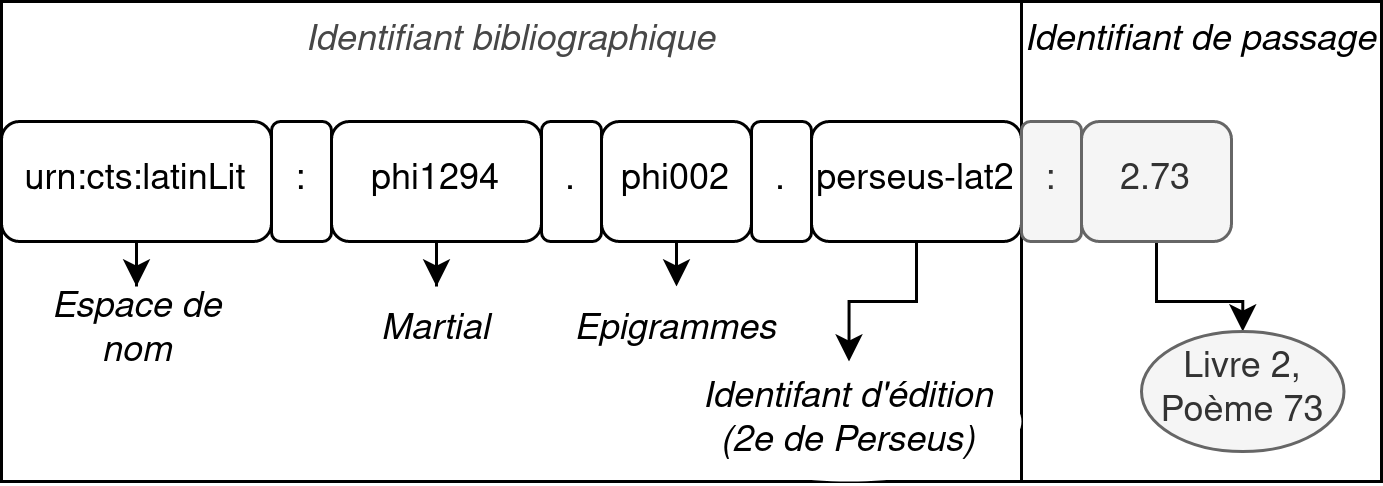
\includegraphics[height=3cm]{figures/chap1/part2/cts-urn.drawio.png}
    \caption{Déconstruction d'un identifiant CTS équivalent au \enquote{Martial, 2, 73}: \texttt{urn:cts:latinLit:phi1294.phi002.perseus-lat2:2.73}}
    \label{fig:chap1:cts_urn}
\end{figure}

% Métadonnées générales (Gillivray ?)
%   -> Reprendre la méthode de datation
% Métadonnées structurelles
%   -> Poser la question de la citabilité et de la section des textes

% Reprendre le travail de Mc Gillivray ici
% La question de la datation
% Poser la question de la citabilité et de la section des textes
% Métadonnées de “lecture”: modèles de citation, niveau de citation recommandé (Introduction du concept de SATU ?)

\subsection{Production et transformations de corpus}

Nous avons défini un cadre théorique à la production de corpus via ses obligations en termes d'éthique scientifique. Il convient désormais de présenter le cadre technique, permettant de réaliser nos objectifs dans les meilleures conditions: obtenir un corpus tel qu'il sera possible d'y retrouver les exemples d'isotopie et d'y faire des recherches lexicographiques. Les conditions de sa production sont donc des conséquences de ces choix: le corpus doit être standardisé et donc en XML-TEI, doit posséder des métadonnées fines, y compris un système d'identification de passages afin de pouvoir revenir à la source ou comparer le texte d'une édition avec une autre. Enfin, il doit avoir une couverture temporelle la plus large possible pour convenir à l'oeuvre d'Adams, qui dépasser chronologiquement Isidore\footnote{Le nombre de textes plus tardifs qu'Isidore est très réduit. On ignorera aussi les sources épigraphiques.}. Nous nous intéresserons ici d'abord à la méthode d'encodage et à l'outillage pour produire ce corpus. Ensuite, nous discuterons de sa compilation, à la fois en tant que meta-corpus et en tant que générateurs de versions inédites de textes. Enfin, nous proposerons une analyse des textes contenus, du point de vue des périodes, des quantités et de la diversité d'auteur.


\subsubsection{Choix techniques: XML TEI et Capitains}

La TEI est une \enquote{grammaire}, en cela, elle a l'avantage d'être partagée par de nombreux projets et d'être compréhensible. Mais elle n'est \enquote{que} descriptive: l'exploitation de sa syntaxe ne peut se faire qu'à travers des outils développés pour elle, qu'ils soient faits sur mesure ou partagés par la communauté. Dans ce contexte, nous avons développé depuis 2013 un ensemble d'outils tournés vers l'exploitation et la description des structures logiques de citations et de leurs identifiants. Cet ensemble d'outils, nommé \textit{Capitains}, est constitué de deux pans: un tourné vers l'encodage et l'organisation de corpus, un second cherchant à valoriser, contrôler et exploiter les données ainsi encodées\footcite{clerice_capitains_2015}. Ce cadriciel démarre sous la tutelle des projets Perseus et Perseids et sur la demande de Bridget Almas, ingénieure principale des deux projets\footnote{Officiellement uniquement de Perseids.}, afin de mettre en place un service de distribution de textes qui permette une maintenance rapide et une citabilité pour CTS\footnote{Ce travail est largement décrit, et plus techniquement qu'ici, dans les articles suivant: \textcite{almas_continuous_2018, clerice_les_2017}}. 

Les \textit{guidelines} Capitains identifient dès leur création deux problèmes importants pour la gestion des corpus de \textit{Perseus}. D'une part, les métadonnées bibliographiques sont particulièrement difficiles à maintenir: chaque fichier du corpus doit contenir des métadonnées sur l'auteur et l'oeuvre, quand bien même ces dernières sont multipliées à l'envie, le corpus étant composé d'auteurs prolixes -- comme Cicéron -- et d'oeuvres représentés par de multiples éditions et traductions.  D'autre part, les textes doivent être eux-mêmes facilement manipulables et répondre à l'ensemble des besoins de l'API CTS, entre autres ceux de la citabilité et de l'obtention automatique de passages via leur identifiant.

Pour le premier problème, celui de la gestion de corpus et de ses métadonnées bibliographiques, on a procédé à l'extraction de ces dernières en dehors du fichier lui-même. En décrivant les auteurs ou les oeuvres hors de celles-ci, la maintenance des informations communes est centralisée et permet de rapidement mettre à jour le catalogue. Pour simplifier encore ce travail, les dépôts \textit{Capitains} doivent suivre une \enquote{syntaxe} pour l'arborescence des fichiers, permettant ainsi de trouver facilement un auteur, ou un oeuvre, parmi plusieurs centaines de fichiers. Avec le recul et l'expérience accumulée au fil des années, cette externalisation est à la fois utile -- la compilation du catalogue est extrêmement rapide car elle ne nécessite pas d'ouvrir de gros fichiers TEI -- mais extrêmement inadaptée à de plus petits corpus, qui souffrent d'avantage de la duplication des efforts (métadonnées d'en-têtes TEI, métadonnées de catalogue \textit{Capitains}).

La seconde partie du problème -- plus intéressante pour nous ici -- s'intéresse à la manière de rendre intelligibles à un programme les structures logiques de citations. Grâce à l'explicitation des rôles et des hiérarchies textuelles des noeuds XML, il est possible de produire par exemple des tables des matières pour un logiciel: le fichier devient donc \textit{machine-actionable}. Or, si l'usage de l'expression \enquote{encodage CTS} peut se trouver chez des chercheurs aguéris comme  L.~Muellner\footcite{muellner2019free}, CTS ne déclare aucun moyen de constituer les données et se déclare même \enquote{\textit{technology independant\footcite{smith_brief_nodate}}}: il faut donc trouver une solution technique, pour des sources TEI, à ce problème. Au moment de la production des \textit{guidelines} Capitains, vers 2014, une seule méthode avait retenu notre attention et semblait offrir une solution à ce problème. Nous discuterons ensuite brièvement d'une seconde option, arrivée en 2021 dans les \textit{guidelines TEI}.

CTS définit le texte comme une structure OHCO extrêmement rigide: le texte est un arbre, dont chaque feuille ou branche est un élément citable construisant son propre identifiant à partir de ceux de l'ensemble de ses ancêtres. Ainsi, le numéro de vers d'un poème de Martial ne peut exister qu'avec la référence de son poème et du livre de ce dernier: 2.72.1 est ainsi l'identifiant du premier vers, du soixante-douzième poème du deuxième livre. CTS requiert des identifiants qu'ils soient uniques et les définit comme inséré dans une séquence et une hiérarchie. Les \textit{guidelines} Capitains jusqu'à leur version 2.0 incluse ne peuvent accepter qu'une structure hiérarchique simple, un arbre dont les branches de citation ne peuvent avoir qu'un seul type d'enfant et un seul squelette de chemin XML (appelé xPath): chaque type de passage ne peut être parent que d'un seul type d'enfant, ici livre, poème, vers. Pour décrire cet arbre de citation, les \textit{guidelines} Capitains font appel aux éléments \texttt{cRefPattern} (\textit{Canonical Reference Pattern}) du \texttt{refsDecl} (\textit{References System Declaration}) des \textit{guidelines} TEI. Les niveaux, décrits les uns après les autres, du plus profond au plus proche de la racine, utilisent un système de xPath et d'expressions régulières pour fournir à la machine tout un outillage pour la compréhension des identifiants (1.2.3 est à tel endroit) ou leur reconstitution (1.2.1, 1.2.2, 1.2.3, etc.), comme dans l'exemple \ref{chap1:xml:cRefPattern}.

\begin{figure}[ht]
    \centering
    \lstset{language=XML}
    \begin{lstlisting}[language=XML]
<refsDecl n="CTS">
    <cRefPattern n="line"matchPattern="(\w+).(\w+).(\w+)"
        replacementPattern="#xpath(/tei:TEI/tei:text/tei:body/tei:div/tei:div[@n='$1']/tei:div[@n='$2']/tei:l[@n='$3'])">
    </cRefPattern>
    <cRefPattern n="poem" matchPattern="(\w+).(\w+)"
        replacementPattern="#xpath(/tei:TEI/tei:text/tei:body/tei:div/tei:div[@n='$1']/tei:div[@n='$2'])">
    </cRefPattern>
    <cRefPattern n="book" matchPattern="(\w+)"
        replacementPattern="#xpath(/tei:TEI/tei:text/tei:body/tei:div/tei:div[@n='$1'])">
    </cRefPattern>
</refsDecl>
    \end{lstlisting}
    \caption{\texttt{refsDecl} des \textit{Épigrammes} de Martial dans le dépôt Github de Perseus. Les niveaux sont déclarés du plus profond (les vers) au plus proche de la racine (les livres). Chaque \textsc{replacementPattern} fournit un xPath où les variables \$1, \$2 ou \$3 sont remplacées via le découpage des identifiants autour des points. Le passage 2.72.1 donnera \$1=2, \$2=72, \$3=1 et donc un xPath \texttt{/TEI/text/body/div/div[@n='2']/div[@n='72']/l[@n='1']}}
    \label{chap1:xml:cRefPattern}
\end{figure}

Depuis 2021, une autre option, beaucoup plus élastique et plus simple à l'utilisation pour les encodeurs comme pour les développeurs, a été mise à disposition dans les \textit{guidelines} TEI\footcite{cayless_introducing_2021}. Cette nouvelle méthode de déclaration permet d'échapper non seulement à la complexité des \texttt{cRefPattern} et de clarifier la hiérarchie entre les système de passages, mais aussi d'intégrer des variations bienvenues dans la ridigité de ceux-ci, en autorisant des systèmes différents de citation. Les \texttt{citeStructure} permettent ainsi de générer nom seulement des arbres de citation mais aussi de les qualifier par des métadonnées, avec une complexité technique beaucoup plus faible que celle des premières options susmentionnées (\textit{cf.} \ref{chap1:xml:citeStructure}).

\begin{figure}[ht]
    \centering
    \begin{adjustbox}{width=0.9\textwidth,keepaspectratio}
    \lstset{language=XML}
    \begin{lstlisting}[language=XML]
<refsDecl n="CTS">
  <citeStructure unit="book" match="/TEI/text/body/div" use="@n">
    <citeData property="http://purl.org/dc/terms/title" use="head"/>
    <citeStructure unit="poem" match="div" use="@n" delim=".">
      <citeStructure unit="line" match=".//l" use="@n" delim="."/>
    </citeStructure>
  </citeStructure>
</refsDecl>
    \end{lstlisting}
    \end{adjustbox}
    \caption{Équivalent de la figure \ref{chap1:xml:cRefPattern} utilisant les déclarations \texttt{citeStructure}. Chaque élément repart de la déclaration parente. \texttt{citeData} permet d'ajouter des qualifications (métadonnées) de chaque passage pour la machine.}
    \label{chap1:xml:citeStructure}
\end{figure}

Mais les \textit{guidelines} Capitains ne sont que la première étape, celle de l'explicitation, dans la gestion des structures logiques de citation: elles ne sont qu'une forme de \enquote{sur-TEI}. L'exploitation de ces structures d'encodage est fournie à travers plusieurs outils dont la principale brique est \textit{MyCapytain}, une librairie fournissant un grand nombre de fonctionnalités \enquote{nues} et sans objectif propre à part celle de rendre plus facile le développement autour des \textit{guidelines}. \textit{MyCapytain} permet \enquote{de mettre en action} les informations fournies par les différentes déclarations citées: dans notre cas, elle nous permet de produire une liste des passages extrêmement détaillées, liant chacune des phrases ou des mots à un identifiant complet du type \texttt{urn:cts:latinLit:phi1293.phi002.perseus-lat2:2.72.1} autour d'un code réutilisable et compréhensible. Le corpus peut être ensuite intégralement appelé et chargé à l'aide de ces quelques lignes\footnote{Le traitement du corpus, du téléchargement des nouvelles versions des corporas à leur lemmatisation en passant par leur découpage en segments identifiés par le système d'URN CTS se retrouve dans les notebooks \enquote{Data Preparation - Corpora}. Ce morceau de code est dérivé librement du notebook \enquote{\textit{Step 1}}.}:

\begin{lstlisting}[language=Python]
import glob
from MyCapytain.resolvers.cts.local import CtsCapitainsLocalResolver

repositories = list(glob.glob(CorporaPathList, recursive=False))
resolver = CtsCapitainsLocalResolver(repositories)
for text in resolver.texts:
    if text.lang == "lat":
        # Traitement du texte
\end{lstlisting}

Avec la complexité que représentent l'encodage des structures logiques de citation, leur interprétation dynamique par des logiciels tiers, et les restrictions produites par les recommandations CTS, la constitution de corpus Capitains est plus à même de contenir des erreurs d'encodage que ne sauraient détecter de simples schémas XML. À travers la TEI comme les \textit{guidelines} Capitains, le texte devient un programme: il est donc capable de contenir des bugs, qui sont de l'ordre de la gestion technique de la donnée, à côté de problèmes d'usages, qui relèvent de la gestion qualitative de la donnée. Nous avons donc introduit des outils de contrôle pour cet encodage particulier qui, en testant automatiquement ce dernier, simplifie la validation \enquote{technique} et laisse ainsi le loisir de s'intéresser principalement à la qualité de ce dernier. C'est pourquoi l'ensemble des textes Capitains peuvent être validés par un outil appelé \textit{HookTest}. Cet outil, en plus d'intégrer des tests de schémas TEI, vérifie que chacun des systèmes de déclaration (1) corresponde à des passages uniques, (2) ne croise pas un autre système de citation, (3) ne produise pas de conflit d'identifiants (\textit{cf.} figure \ref{fig:annx:digiliblt-hooktest} en annexe).

\begin{figure}
    \centering
    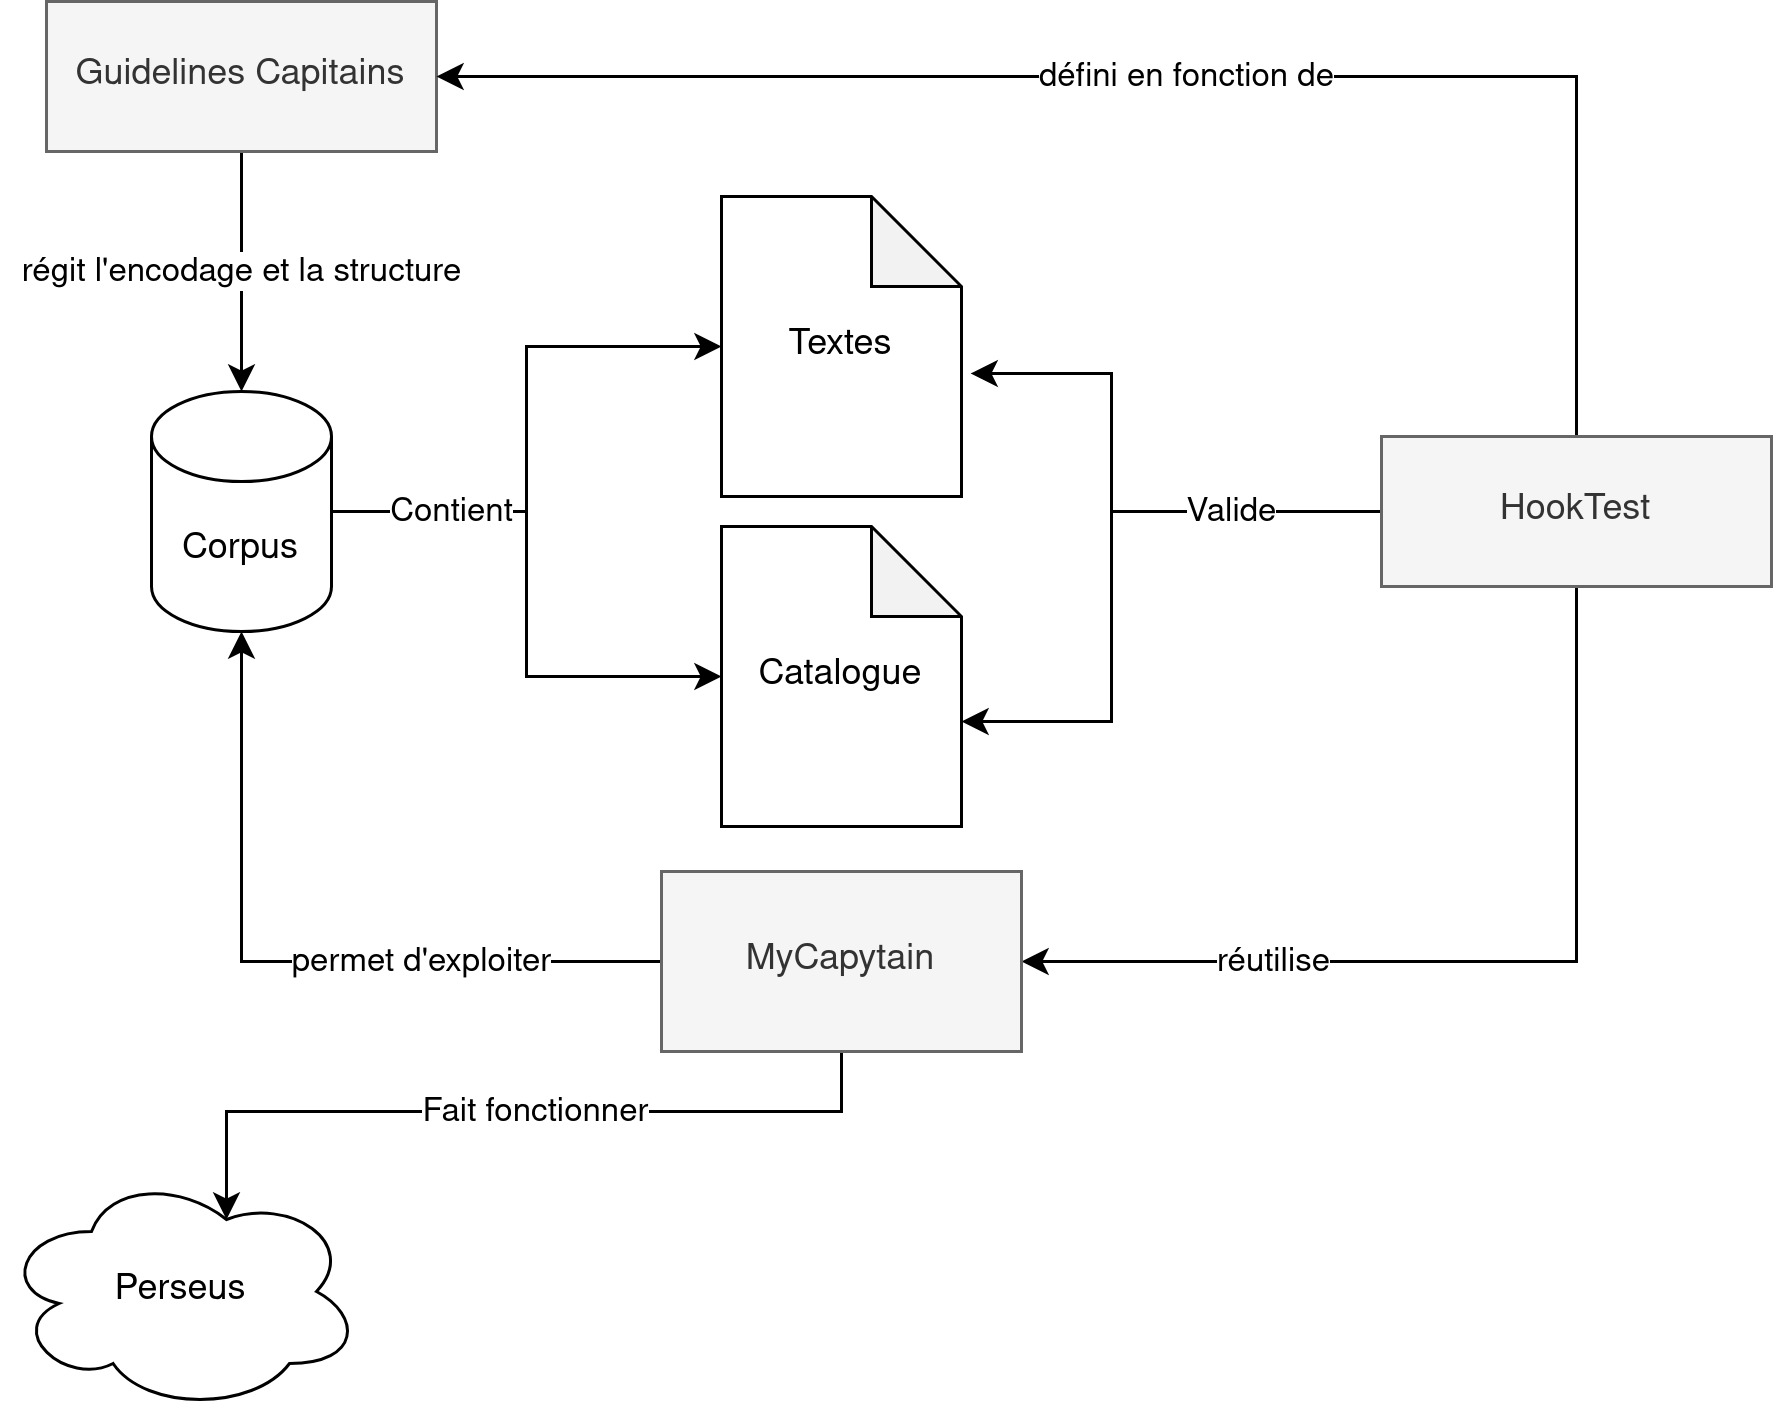
\includegraphics[width=\textwidth]{figures/chap1/part2//capitains.png}
    \caption{Mode de fonctionnement de \textit{Capitains}. \textit{MyCapytain} est une brique commune  l'ensemble des programmes python du monde \textit{Capitains}, elle permet de faire fonctionner autant \textit{HookTest} que \textit{Nautilus}, l'application derrière les serveurs de textes de \textit{Perseus}.}
    \label{fig:chap1:Capitains}
\end{figure}

% Dans la production de corpus, HookTest se situe à la fois comme un outil à utiliser individuellement, pendant la création de fichiers TEI, mais aussi de manière continue dans la vie du corpus. Nos corpus
%Le contrôle qualité des données est un pré-requis important à la construction d'application ou d'analyse. 



\subsubsection{Méthode de compilation, conversion et sources des corpus}

Tous ces choix mènent enfin à la compilation d'un meta-corpus permettant de retrouver et créer notre corpus exemplier. Cette phase de collection et de production est un processus itératif, conditionné à la fois par la mise à disposition de nouvelles sources au format numérique, par la gestion de priorité d'acquisition en fonction de la rencontre d'oeuvres chez Adams mais indisponibles dans les corpus au format CapiTainS, et par les opportunités de traitement et d'externalisation de cette mission. Nous discuterons d'abord du travail effectué sur les corpus pré-existants et adaptés à notre cadre technique, puis à l'adaptation de corpus existants.

En effet, l'opportunisme et l'économie d'énergie régissent d'abord notre collecte: nous pouvons commencer par adopter les corpus qui sont déjà adaptés à nos pré-requis techniques. \textit{Capitains} ayant été adopté par la sphère de \textit{Perseus}, et presque uniquement par celle-ci, ce projet et son alter-ego \textit{Open Greek and Latin} sont les premières sources de notre corpus. Pour autant, chacun des corpus disponibles dans ces projets (\textit{Canonical Latin Literature} de \textit{Perseus}, \textit{CSEL} et \textit{PL} d'\textit{OGL}) pose un problème spécifique.

Pour reprendre l'historique de la production de ces corpus et projets, \textit{Perseus} n'avait pas, au début de nos travaux de recherche, converti l'ensemble de ses textes aux \textit{guidelines Capitains}, encore moins pour ses textes latins. De 2013 à 2016, l'ensemble des conversions de textes latins des dépôts Perseus datant d'avant l'obtention de la chaire à Leipzig avait été réalisé par nos soins, sans que cela soit une mission prioritaire du laboratoire. La majeure partie des efforts de l'équipe se concentre d'abord sur les textes du CSEL puis sur les textes de la PL. En avril 2017, au moment de notre départ de Leipzig, le corpus ne contenait que 390 textes convertis sur 674, traductions inclues, pour un total d'environ 5,07 millions de mots en latin\footcite{travis_hook_2017, travis_hook_2017_logs}. En décembre 2021, ce total est monté à 418 textes sur 686, avec une augmentation de plus d'un million de mots\footnote{6~159~948 mots latins pour êtres précis, d'après \textcite{travis_hook_2021_logs}}. L'une des sources principale de cette augmentation est la conversion de l'ensemble du corpus de Cicéron, produite dans le cadre de notre méta-corpus. Ces modifications des données de \textit{Perseus}, aussi justes soient elles, ont besoin d'être validées par l'équipe actuelle du projet et donc de rentrer dans le calendrier de production des données de Perseus. Sur ce dernier point, on notera qu'en décembre 2021 deux conversions effectuées pour le méta-corpus\footcite{noauthor_pull_nodate} étaient encore en attente de validation par l'équipe actuelle du projet: elles ne rentraient pas dans le calendrier de rétro-conversion des sources, principalement tourné vers le grec et les traductions\footnote{Il n'est en aucun cas question ici de jeter la pierre sur d'anciens collègues, mais de mettre en avant les problèmes que peuvent poser parfois ce genre de collaboration, à travers l'existence de priorités, d'attentes et de missions différentes.}. 

Un cas particulier de conversion pour le corpus principal de \textit{Perseus}, \textit{Canonical Latin Literature}, est celle des \textit{Annales} de Tacite. Ce texte -- dont \textit{Perseus} possédait plusieurs éditions -- a été victime d'un problème de conversion entre les diverses versions de la plate-forme qui a donné lieu à la segmentation involontaire de plusieurs éditions du texte en quarante-sept oeuvres sans distinction des regroupement originaux\footcite{noauthor_canonical_latinlitphi0660phi003perseus_lat2xml_nodate, clerice_phi0914phi001lat2_nodate}. Sa \textit{capitainisation} est impossible à partir des fichiers \textit{open source} trouvables dans les dépôts du projet, car elle demande alors une connaissance de l'historique des migrations pour en déduire l'origine des problèmes et un travail minutieux de transformation d'une TEI P4 vers une TEI P5 Capitains. C'est à travers une collaboration entre d'anciens employés et des employés actuels que cette conversion a été rendue possible.

Outre le corpus original \textit{Canonical Latin Literature}, Perseus et le projet \textit{Open Greek and Latin} ont mis à disposition deux autres corpus: le CSEL et la PL. Ces deux derniers ont la particularité d'être des corpus extrêmement récents dans l'histoire de Perseus, produits majoritairement via OCR et dont la structuration en XML TEI a été externalisée à une entreprise n'étant pas composée de latinistes ou d'hellénistes mais d'encodeurs de documents administratifs. Cette méthode de production de données a engendré deux grands problèmes. D'une part, l'OCR peut présenter des erreurs, anodines souvent, particulièrement problématiques pour notre étude parfois. On notera par exemple l'erreur répétée de segmentation d'\textit{oraculus} en deux mots (\textit{ora} et \textit{culus}) suite à la non résolution d'une hyphénation qui n'avait plus lieu d'être dans le document XML, mais aussi de \textit{sae-culum}, d'\textit{o-culus}, de \textit{claui-culus}, \textit{taberna-culum}, etc\footnote{Quelle ne fut pas notre surprise quand nous trouvions, par moteur de recherche, un grand nombre d'emploi de \textsc{culus} chez Augustin d'Hippone.}. D'autre part, l'encodage des structures logiques de citation a pu poser des problèmes, car sa formalisation typographique peut fluctuer d'une impression à l'autre, d'autant plus sur des périodes de productions comme celle de la CSEL (plus d'un siècle), et il peut être difficile de faire la différence entre un numéro de ligne, un numéro de section, etc. Cette reproduction de l'information demande alors à la fois une compréhension des mécanismes d'édition et de langues, afin de séparer les identifiants de section du texte: il ne s'agit pas seulement de reconnaître les sauts de lignes qui sont des vers ou des changements de paragraphes, mais aussi le rôle du paratexte qui les accompagne.

La constitution de ces corpus a aussi eu le malheur d'avoir lieu pendant la formalisation des \textit{guidelines} Capitains. Il a donc fallu, après la réception des données, non seulement reprendre les structures logiques mais aussi intégrer les informations requises pour leur exploitation. Ce travail a été achevé pour la CSEL au cours de l'année 2017 par Matt Munson, employé de Leipzig à cette époque, mais pas pour la PL, la laissant \enquote{en friche} du point de vue de sa compatibilité avec les outils de l'écosystème \textit{Perseus}. Cet abandon du corpus, au moins momentané, est un exemple supplémentaire du changement politique et économique de la production de corpus de \textit{Perseus}. Le projet \textit{First Thousand Years of Greek} du CHS apporte plus de fonds, les textes de la patrologie latine sont disponibles par ailleurs sur d'autres plate-formes: le projet change de priorités de production de corpus. Un seul corpus supplémentaire est né depuis 2017 en latin: le corpus OGL/Latin. Il contenait deux textes au moment de la compilation du meta-corpus.

CSEL et canonical-latinLit mis ensemble, le corpus représente environ douze millions de mots, dont les épicentres thématiques et chronologiques sont respectivement les pères de l'Église de l'antiquité tardive et la littérature classique de la Rome pré-chrétienne. Il reste alors pour couvrir les périodes présentes chez Adams, en plus de quelques textes non convertis chez \textit{Perseus}, trois pans:

\begin{enumerate}
    \item l'épigraphie. Elle est intégralement ignorée dans notre corpus pour des raisons évoquées plus tôt, comme le problème important de sa lemmatisation.
    \item la période tardive non-chrétienne, en particulier les littératures médicales (importants pour notre recherche) et celles des grammairiens.
    \item la littérature de la période classique peu connue ou peu étudiée avant le niveau master en lettres classiques: \textit{Perseus} se concentre d'abord historiquement sur les corpus les plus communs pour rendre leur accès plus facile. 
\end{enumerate}

Pour le deuxième comme pour le troisième pan, la règle principale pour l'intégration de textes au meta-corpus a été leur mention par Adams dans son ouvrage: tout texte dans les bornes chronologiques mentionnées -- c'est-à-dire avant la mort d'Isidore de Séville -- a fait l'objet d'une recherche quant à la disponibilité d'une édition numérique correspondante dans un corpus tiers. Dans le cas où le code pour la conversion d'une édition XML-TEI, HTML ou plein texte était facilement réutilisable pour convertir d'autres oeuvres similaires d'un même site, nous ajoutions à l'oeuvre mentionnée par Adams les oeuvres similaires convertissables à bas coût. Ces conversions ont été mises à disposition dans deux corpus distincts: pour les oeuvres du projet \textit{DigilibLT}, projet encore actif et centré sur un des angles morts des corpus Perseus, la littérature tardive non chrétienne, un corpus miroir \textit{DigilibLT-Capitains}\footcite{Clerice_Digital_Latin_Library_2021} a été mis en développement par nos soins; pour les autres oeuvres, issues de sources diverses (\textit{cf.} table \ref{tab:chap1:corpusutilises}), un corpus sobrement nommé \enquote{\textit{Lasciva Roma - Additionnal Texts}}\footcite{Clerice_Corpora_of_rare_2021} a vu le jour. Le premier compte 103 textes\footnote{sur 216 téléchargés de \textit{DigilibLT}} et 2,8 millions de mots, le second 134 textes et 3,8 millions.


\begin{table}[h]
    \centering
    \begin{tabular}{lr}
        \toprule
        Corpus numérique ou édition numérique utilisée & Fréquence \\
        \midrule
         OBI\footnotemark            & 73 \\
         Lacus Curtius\footnotemark         & 18 \\
         Corpus Corporum\footnotemark & 12 \\
         Horatius.net\footnotemark    & 12 \\
         The Latin Library\footnotemark   &  4 \\
         Musisque Deoque\footnotemark &  3 \\
         Perseus        &  3 \\
         Remacle\footnotemark        &  2 \\
         ALIM\footnotemark           &  1 \\
         Lesley Bolton\footnotemark         &  1 \\
         Latin Law Library\footnotemark    &  1 \\
         Monumenta Germanica Historica\footnotemark            &  1 \\
         Corpus Scriptorum Latinorum\footnotemark            &  1 \\ \midrule
         Éditions originales à partir d'OCR    &  2 \\
        \bottomrule
    \end{tabular}
    \caption{Source des corpus utilisés. Deux sortent du lot. OBI présente 73 éditions, un nombre surgonflé: il y a 73 livres pour la \textit{Vulgate} d'après CTS). Nous remercions chaleureusement Lesley Bolton, docteure canadienne, de nous avoir permis de réutiliser son travail de thèse pour en faire une édition TEI. Les éditions originales à partir d'OCR ont été produites à partir des données d'\textit{Internet Archive}.}
    \label{tab:chap1:corpusutilises}
\end{table}
\footnotetext{\textcite{barry_schein_open_1994}}
\footnotetext{\textcite{lomarcan_lacuscurtius_1999}}
\footnotetext{\textcite{roelli2014corpus}}
\footnotetext{\textcite{horatiusnet}}
\footnotetext{\textcite{carey_latin_1998}}
\footnotetext{\textcite{gelderblom_musisque_2008}}
\footnotetext{\textcite{philippe_remacle_site_2008}}
\footnotetext{\textcite{d2019alim}}
\footnotetext{\textcite{bolton_edition_2015}}
\footnotetext{\textcite{lassard_roman_2001}}
\footnotetext{\textcite{noauthor_openmgh_nodate}}
\footnotetext{\textcite{csl}}

Pour le troisième point, un texte fondamental pour notre recherche est absent des corpus Perseus: les \textit{Priapées}\footcite{Clerice_Digital_edition_of_2020}. Il s'agit d'un ensemble de poèmes plutôt courts et centrés autour de la personnalité de Priape, dieu gardien des vergers dont l'arme principale est un sexe en érection. Il est constitué de deux blocs, une partie de ses poèmes y ayant été ajouté par analogie au cours des éditions du texte\footcite{callebat_les_2008}. Pour la mettre à disposition, nous avons réutilisé le texte et les traductions de R. F. Burton et L. C. Smithers de 1890\footcite{burton_priapeia_1890} comme première version du texte. Cette base de texte nous a évité de passer par la fastidieuse case de l'OCR, de sa correction et de la qualification de ses lignes en vers, poèmes ou notes de bas de page. Nous l'avons ensuite adapté en fonction de l'édition scientifique d'Emil Baehrens paru chez Teubner\footcite{baehrens_poetae_1910}. Ce texte a été intégralement traduit pour la présente recherche et annoté linguistiquement en lemme et en morpho-syntaxe: cette phase d'annotation a permis de relire intégralement le texte, et de le comparer avec l'édition de Louis Callebat paru en 2012 aux Belles lettres et dont nous avons utilisé la réimpression de 2017\footcite{callebat_priapees_2012}. Si les variations entre les deux éditions sont faibles, on a préféré donner en apparat critique quelques choix de l'éditeur français quand elles respectaient l'intégralité des manuscrits là où l'éditeur allemand en produisait une minoritaire. Comme la majeure partie des éditions de Perseus, cette édition numérique des Priapées a plus pour vocation de donner un texte qu'une édition critique, hormis ces quelques notes importées de la comparaison avec l'édition la plus récente.

\begin{figure}
    \centering
    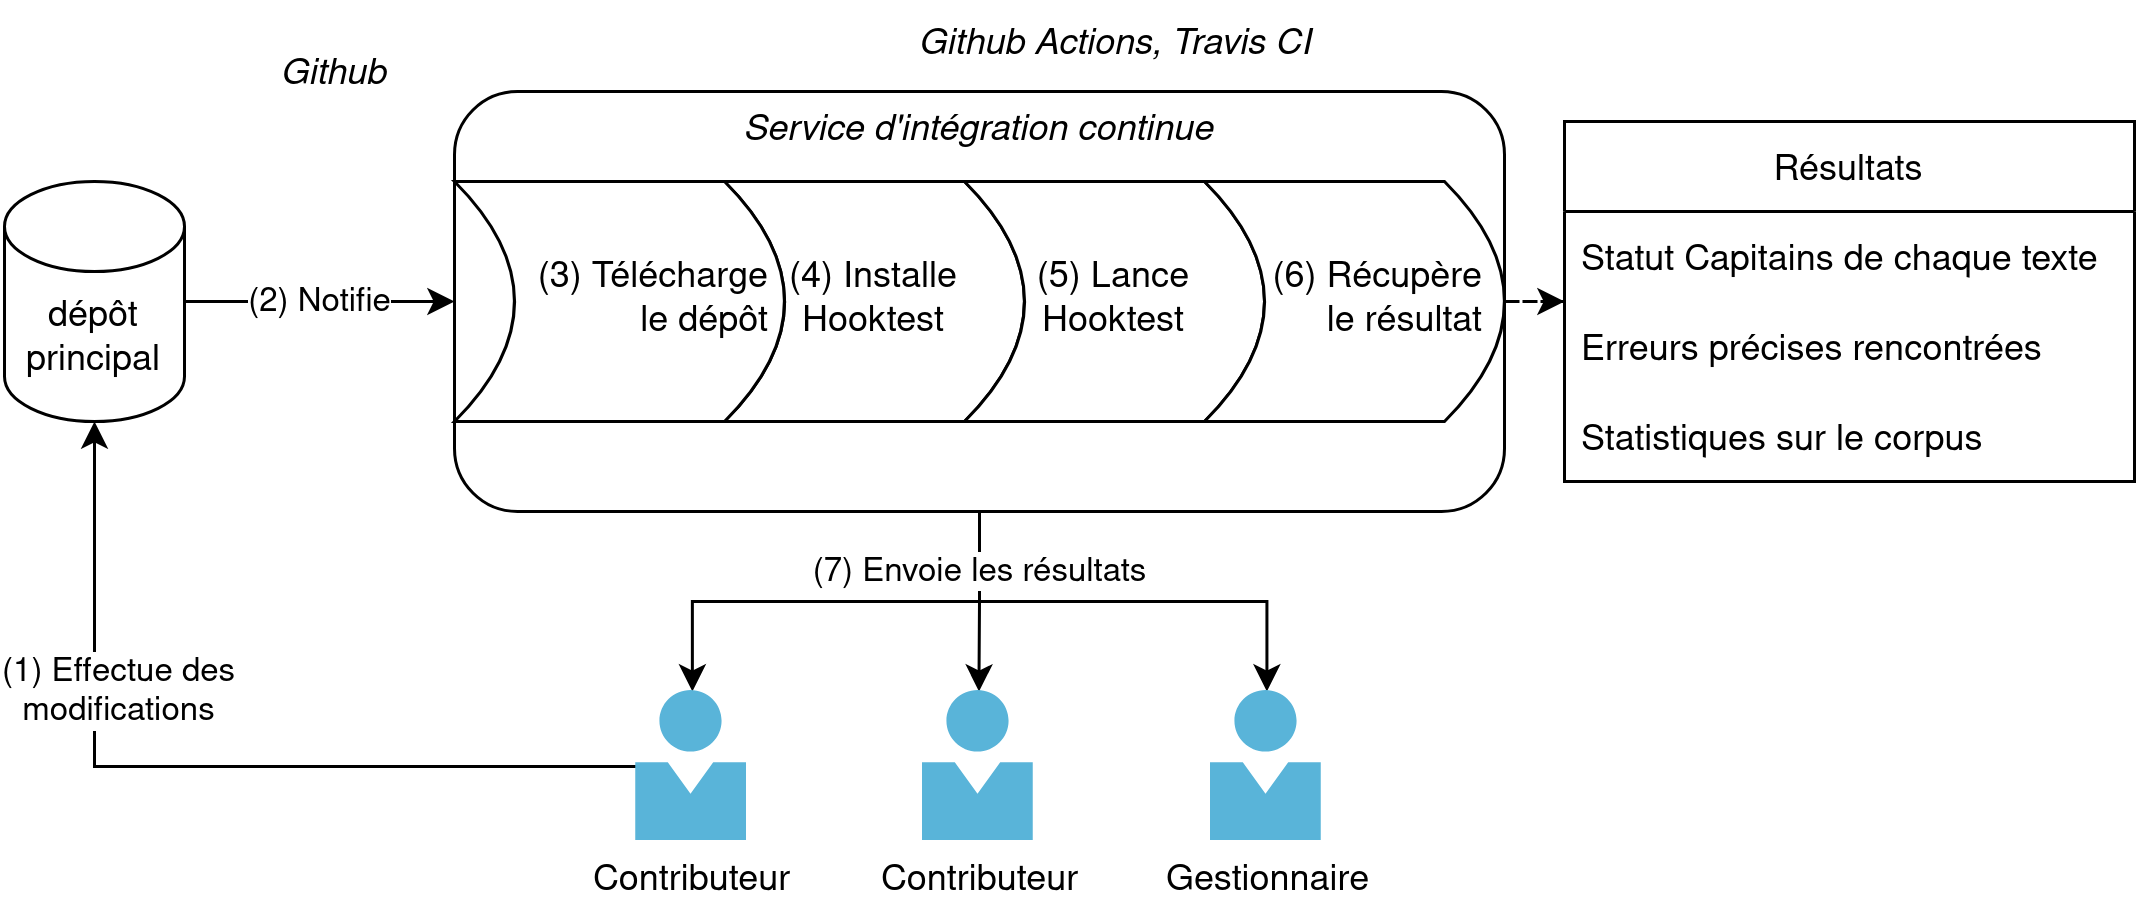
\includegraphics[width=\linewidth]{figures/chap1/part2/hooktest.png}
    \caption{Processus automatisé}
    \label{fig:chap1:ci}
\end{figure}

Une partie du travail sur \textit{DigilibLT-Capitains} et la majeure partie de la conversion de Tacite ont été réalisé dans le cadre de devoirs fournis aux étudiants et étudiantes des master \enquote{Technologies Numériques Appliquées à l'Histoire} (TNAH) et \enquote{Humanités Numériques} de l'ENC et de PSL. Dans le cadre de l'apprentissage des outils de versionnage Git, cinquante-six éditions du projet italien ont été \enquote{capitainisées}, les textes retenus ayant été choisis librement par les étudiants. Cet exercice permettait à la fois de comprendre les enjeux de la collaboration sur plate-forme numérique, avec une dizaine de collaborateurs travaillant sur des données partagées, ses bonnes pratiques et la gestion des contrôles qualités. En effet, \textit{HookTest} permet aussi d'être utilisé comme un outil de contrôle automatique des corpus sur des plate-forme comme Github dans le cadre d'intégration continue, c'est-à-dire dans le cadre de tests automatisés et décentralisés lancés à chaque modification du dépôt contenant les données (\textit{cf.} figure \ref{fig:chap1:ci}).
% Ces corrections demandent à la fois une compréhension de la langue et des règles de mise en page. 
% Description des corpus ciblés et du processus itératif d'adaption du corpus

% Enfin, statistiques sur le corpus.
    % Statistiques sur les corpus Perseus et autres
    % La conversion de DigilibLT
    % Présentation des corpus Lasciva Roma
    %% Priapées
    %% Additional-Texts
    
\subsubsection{Description du meta-corpus final}

Le meta-corpus final est formé des six corpus \textit{open-source} et libres de droit mentionnés pour un total d'une vingtaine de millions de mots (\textit{cf.} table \ref{tab:chap1:corpora}). Il est constitué de 204 auteurs ou regroupements d'oeuvres (par exemple, le \textit{Nouveau Testament} compte comme un regroupement de textes) pour 853 oeuvres. Tous les textes cités par le TLL ou par Adams n'ont pas pu être ajoutés au corpus: on note par exemple l'absence des \textit{Declamatio minores} de Quintilien, des commentaires de Donat ou de textes du \textit{Corpus Grammaticorum Latinorum}. Nous avons suivi les principes de production de corpus originaux de Perseus, à savoir de ne pas inclure les auteurs fragmentaires: majoritairement collectés via des citations chez d'autres auteurs, leur introduction pourrait introduire du bruit. 

En dehors des manques particuliers à la collecte ou à l'histoire des corpus réutilisés, notre corpus présente des caractéristiques assez attendues d'un corpus de sources anciennes et littéraires. Il est constitué majoritairement d'auteurs dont on ne possède qu'une seule oeuvre (près de 120 auteurs sont dans ce cas) avec quelques auteurs extrêmement prolifiques, comme Augustin et Cicéron avec une soixantaine d'oeuvres (\textit{cf.} \ref{fig:chap1:oeuvres-par-auteur}). Les textes sont assez courts: les trois quarts font moins de 20~000 mots (\textit{cf.} table \ref{tab:chap1:mots-par-textes}). Quatre-vingt textes font moins de mille mots (10\% du corpus) tandis que quanrante neuf en font plus de cent mille. Les textes les plus grands atteignent le million de mots (\textit{cf.} \ref{fig:chap1:mots-par-texte}).

Chaque corpus du meta-corpus concerne une période qui lui est propre (\textit{cf.} figure \ref{fig:chap1:mots-par-corpus}): \textit{Canonical Latin Literature} de \textit{Perseus} propose des oeuvres majoritairement issues de la période classique, de -254 à 150 de notre ère. Il connaît une légère production supplémentaire aux alentours du IVe siècle avec les oeuvres de Jérôme et d'Ausone, inclues par l'équipe du projet pour des raisons pédagogiques. Le deuxième grand corpus, le CSEL, couvre la période de 300 à 950 avec les pères de l'Église. Le corpus \textit{DigilibLT} est constitué d'oeuvres écrites principalement entre la fin du IIIe siècle au Ve. Au contraire des autres corpus, \textit{Additional Texts} ne présente pas d'homogénéité dans sa production: il est le fruit d'un \enquote{remplissage des manques} et génère donc des inégalités de tailles en fonction des périodes. Il connaît deux pics importants: le premier est formé de la rédaction de la \textit{Vulgate} et des commentaires de Servius pendant le IVe siècle; au Ve siècle, le second pic est constitué d'un seul texte massif, le \textit{Code Justinien}.

\afterpage{%
\begin{table}
\begin{minipage}{.4\linewidth}%
        \centering
        \resizebox{\textwidth}{!}{%
        \begin{tabular}{lr}%
            \toprule
            Corpus                         & Version \\ \midrule
            PerseusDL/canonical-latinLit & 0.0.843 \\
            OpenGreekAndLatin/csel-dev   & 1.0.223 \\
            lascivaroma/priapeia         & 1.1.18  \\
            lascivaroma/additional-texts & 1.0.193 \\
            lascivaroma/digiliblt        & 0.0.64  \\
            OpenGreekAndLatin/Latin      & v1.11.0 \\ \bottomrule
        \end{tabular}%
        }
        \caption{Corpus utilisés pour la formation du meta-corpus de sources.}
        \label{tab:chap1:corpora}
\end{minipage}%
\hfill
\begin{minipage}{.56\linewidth}%
        \centering
        \resizebox{\textwidth}{!}{%
        \begin{tabular}{l|rr|rr}
            \toprule
                      Auteur &      Mots &  Rang      &  Oeuvres &  Rang         \\
            \midrule
                    Augustin & 2~566~421 &          1 &       68 &             2 \\
                   Justinien & 1~430~321 &          2 &        2 &            62 \\
                     Cicéron & 1~389~163 &          3 &       60 &             3 \\
                      Jérôme &   879~855 &          4 &        9 &            19 \\
                     Servius &   717~622 &          5 &        4 &            34 \\
                    Ambroise &   685~483 &          6 &       19 &            10 \\
                  Tertullien &   678~635 &          7 &       50 &             4 \\
                   Tite-Live &   614~940 &          8 &        1 &            87 \\
                     Vulgate &   603~091 &          9 &       73 &             1 \\
                     Sénèque &   525~489 &         10 &       27 &             7 \\ 
                            \multicolumn{5}{c}{...}                \\
                      Plaute &   233~258 &         23 &       20 &             9 \\
            Histoire Auguste &   128~128 &         35 &       30 &             5 \\
                      Ausone &    68~418 &         67 &       29 &             6 \\
              Cornélis Népos &    33~604 &         89 &       25 &             8 \\
            \bottomrule
        \end{tabular}%
        }
        \caption{Auteurs ou groupes de textes les plus importants en oeuvres et en mots, classés par le nombre de mots.}
        \label{tab:chap1:rang-auteurs}
\end{minipage}
\end{table}
\begin{figure}
    \centering
    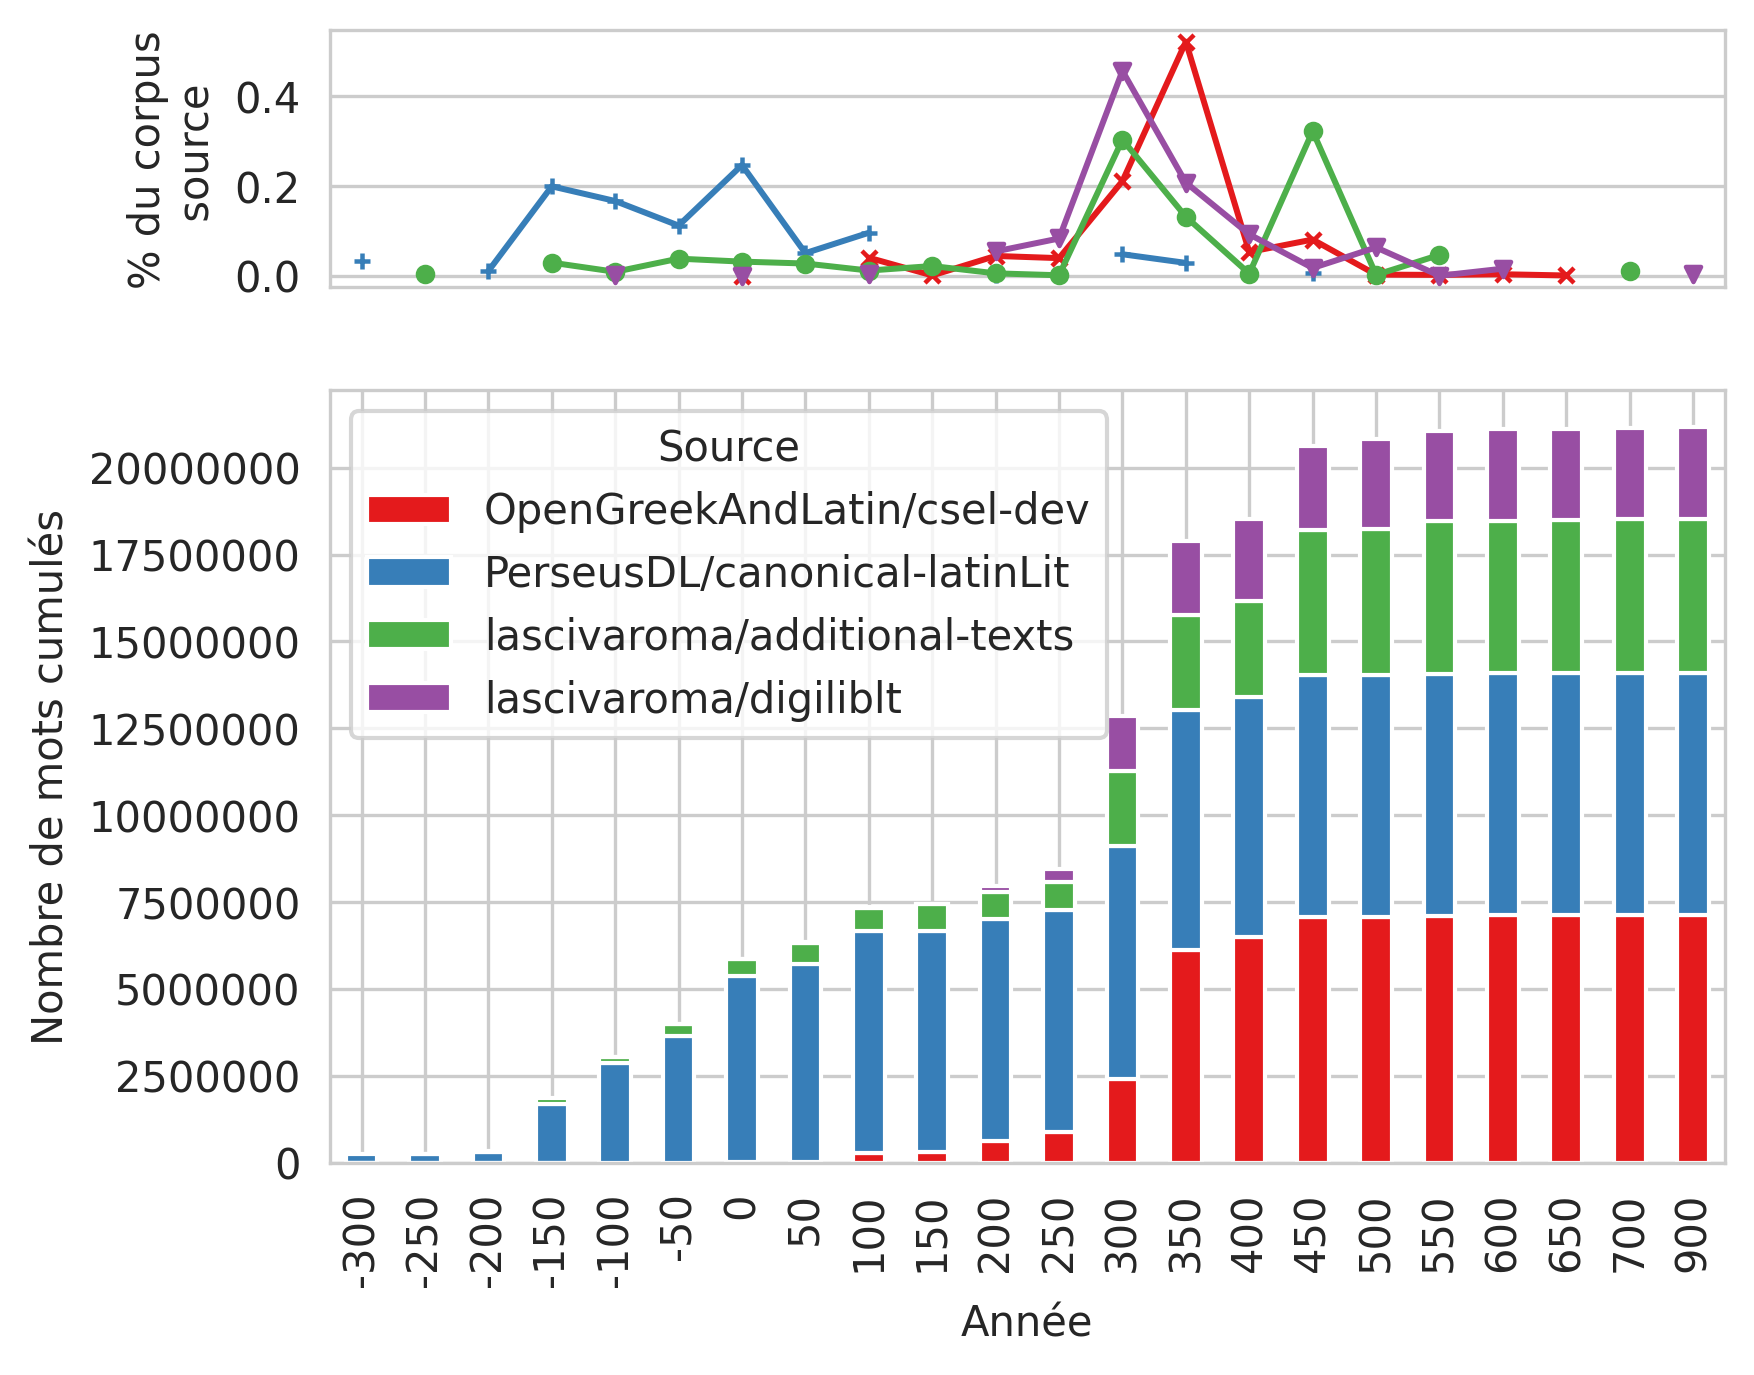
\includegraphics[width=.9\linewidth]{figures/chap1/part2/motsPaCorpus.png}
    \caption{Évolution de la taille du meta-corpus par corpus et par demi-siècle. La partie supérieure du graphe présente les pourcentages relatifs à chaque corpus, la partie inférieure les valeurs absolues en nombre de mots.}
    \label{fig:chap1:mots-par-corpus}
\end{figure}
\clearpage
}

Le meta-corpus contient par ailleurs deux grandes périodes de rédaction, correspondant à deux phénomènes bien identifiés par les historiens de la littérature (\textit{cf.} \ref{fig:chap1:accum-mot}). On a d'une part la littérature dite classique, allant de la fin de la République au règne des Antonins à la fin du Ier siècle de notre ère: elle est constituée -- entre autres -- du graphomane Cicéron, des philosophes Sénèque et Lucrèce, des poètes augustéens et de l'apogée du genre élégiaque, des épopées latines les plus connues, et se termine avec les écrivains Martial, Juvénal et Pline le Jeune. Ces siècles ont été consacrés par l'enseignement du latin à travers le thème, dont la langue est calquée sur les styles césariens et cicéroniens, et l'études des grands classiques comme l'\textit{Énéide} de Virgile et les \textit{Annales} de Tacite\footnote{Il suffit de voir que l'\textit{Anthologie de la littérature latine} de J. Gaillard et R. Martin s'arrête à Apulée (IIe siècle) et ignore l'ensemble de la littérature chrétienne et tardive pour se rendre compte de la focalisation de la réception sur cette période de la littérature. \textcite{gaillard_anthologie_2005}}. Cette période représente un peu moins de la moitié du corpus avec près de dix millions de mots. 

La deuxième période de production massive est ce que Fredouille et Zhenacker appelle \enquote{l'âge d'or de la patristique}\footcite{fredouille}: avec la reconnaissance officielle du christianisme, on assiste à la rédaction des oeuvres d'Hilaire, Ambroise, Augustin et de Jérôme, dont la production -- partiellement représentée dans notre corpus -- correspond à 20,7\% du meta-corpus complet en nombre de mots et 12,5\% en nombre de textes. D'autres auteurs, aux quantités minuscules par rapport à celles des quatre Pères, restent majeurs pour notre recherche: ainsi, le IVe siècle est aussi le siècle d'Ausone, et donc du \textit{Centon Nuptial}, ré-arrangement littéraire des vers de Virgile visant à raconter un mariage et la première nuit des mariés. C'est aussi le siècle des grammairiens et des commentaires: on y retrouve l'oeuvre de Donat, de Servius et, suivant les datations, des \textit{Adnotationes super Lucanum}. Les commentaires peuvent avoir une grande importance pour la compréhension des textes anciens ou du moins de leur réception, et, en termes d'approche quantitative, permettent d'ajouter du contexte aux passages originaux.

Pour ce qui est des manques, ils peuvent être particulièrement compliqués à quantifier. Si l'on en croit le nombre de textes convertis du DigilibLT, il y aurait au moins autant de textes tardifs hors-patristique absents que présents de notre corpus. Pour la patristique, le \textit{Corpus Corporum} fournit une taille pour chaque corpus: la patrologie latine serait formée de quatre-vingt huit millions de mots. Ce chiffre doit être pris comme un ordre de grandeur, car les documents XML de la PL du projets fourmillent de citations en plein texte du type \enquote{(Joan. XV, 17).}, représentant un bruit important pour le décompte de mots. Il reste qu'avec ce nombre, plus de quatre fois la taille de notre corpus, il est certain que nous avons des manques: Jérôme y est représenté par 2,5 millions de mots pour 105 oeuvres (en ne comptant que les oeuvres attribuées assurément par le projet), tandis que le méta-corpus culmine à 880~000 mots pour 9 oeuvres (\textit{cf.} \ref{tab:chap1:rang-auteurs}). La conversion et la collecte des textes ayant été guidées par les citations du TLL et d'Adams, ces auteurs sont sous-représentés.


Pour la période classique, nous bénéficions du travail du \textit{Perseus Catalog}\footcite{babeu2019perseus} et du PHI. Projet enfant de \textit{Perseus}, le catalogue, dirigé par Alison Babeu, a pour vocation de répertorier les auteurs, oeuvres, éditions et traductions des auteurs antiques, et tout particulièrement celles tombées dans le domaine publiques. Ce catalogage s'accompagne souvent de liens vers des textes disponibles sous formes de numérisations PDF sur les plate-formes comme \textit{Google Book}, \textit{Internet Archive} ou \textit{Hathi Trust}. Il est complété du nombre de mots quand l'oeuvre est disponible sur le PHI. Ce décompte, visible en figure \ref{fig:chap1:accum-mot-diff-perseus-catalog}, permet d'estimer qu'il manque -- au plus -- quelques centaines de milliers de mots au plus sur la période classique. Mais tout comme les chiffres de la PL, il est à interpréter avec précaution: en étudiant les auteurs dont les oeuvres sont sous-représentées (\textit{cf.} figure \ref{fig:chap1:ecarts-auteurs}), nous avons trouvé qu'Ovide aurait près de deux cent mille mots de moins dans notre meta-corpus que chez le PHI. Or, Ovide n'est pas l'auteur d'un très grand nombre d'oeuvres ou de recueil, et un tel manque ne pourrait être que la trace de l'oubli d'un classique par \textit{Perseus} dont le projet même était de mettre à disposition les textes couramment étudiés. En cherchant les données manquantes, il s'est avéré que le texte incriminé est une oeuvre mineure, \textit{l'Epicedion Drusi}, un poème de 474 vers dont le nombre de mots est évalué à tord à plus de deux cent vingt mille mots par le catalogue\footcite{clerice_catalog_dataphi0959phi015_2021}. L'écart qui sépare notre meta-corpus du corpus du PHI pourrait donc être moindre que ce qui est affiché par le \textit{Perseus Catalog}. Il reste probable que pour Cicéron (dont les oeuvres complètes ne sont pas toutes présentes sur Perseus), Sénèque (dont quelques ouvrages manquent) et Quintilien (dont il nous manque au moins les \textit{Declamatio Minores}) soient véritablement parcellaires dans le meta-corpus.

Pour conclure, nous faisons face à un meta-corpus varié dont le caractère incomplet est dû en partie aux critères initiaux, à savoir la possibilité d'exploiter mécaniquement les ressources textuelles via une explicitation de leurs structures. S'il devait être compléter, les tâches suivantes devraient être réalisées en priorité:
\begin{itemize}
    \item la conversion complète des oeuvres du \textit{DigilibLT};
    \item la conversion des textes de la patrologie latines dont les auteurs précèdent ou sont contemporains d'Isidore de Séville;
    \item la conversion et l'obtention des textes des grammairiens latins, dont le corpus n'a pas pu être obtenu à temps, soit à travers le \textit{Corpus Grammaticorum Latinorum}, dont les sources sont réutilisées par le C\textit{orpus Corporum}, soit à travers le projet \textit{HyperDonat};
    \item la création d'éditions \enquote{fac-similaires} simples, à la \textit{Perseus}, pour les textes des auteurs classiques manquants, au premier titre desquels figurent Cicéron et Quintilien.
\end{itemize}
Ces recommandations sont par ailleurs dépendantes de l'évolution des techniques de lemmatisation, dont l'adaptation aux textes documentaires et épigraphiques nous pousserait à recommander d'incorporer, surtout pour notre thématique, les inscriptions et graffitis, dont ceux de Pompei.


\afterpage{%
\begin{figure}
    \centering
    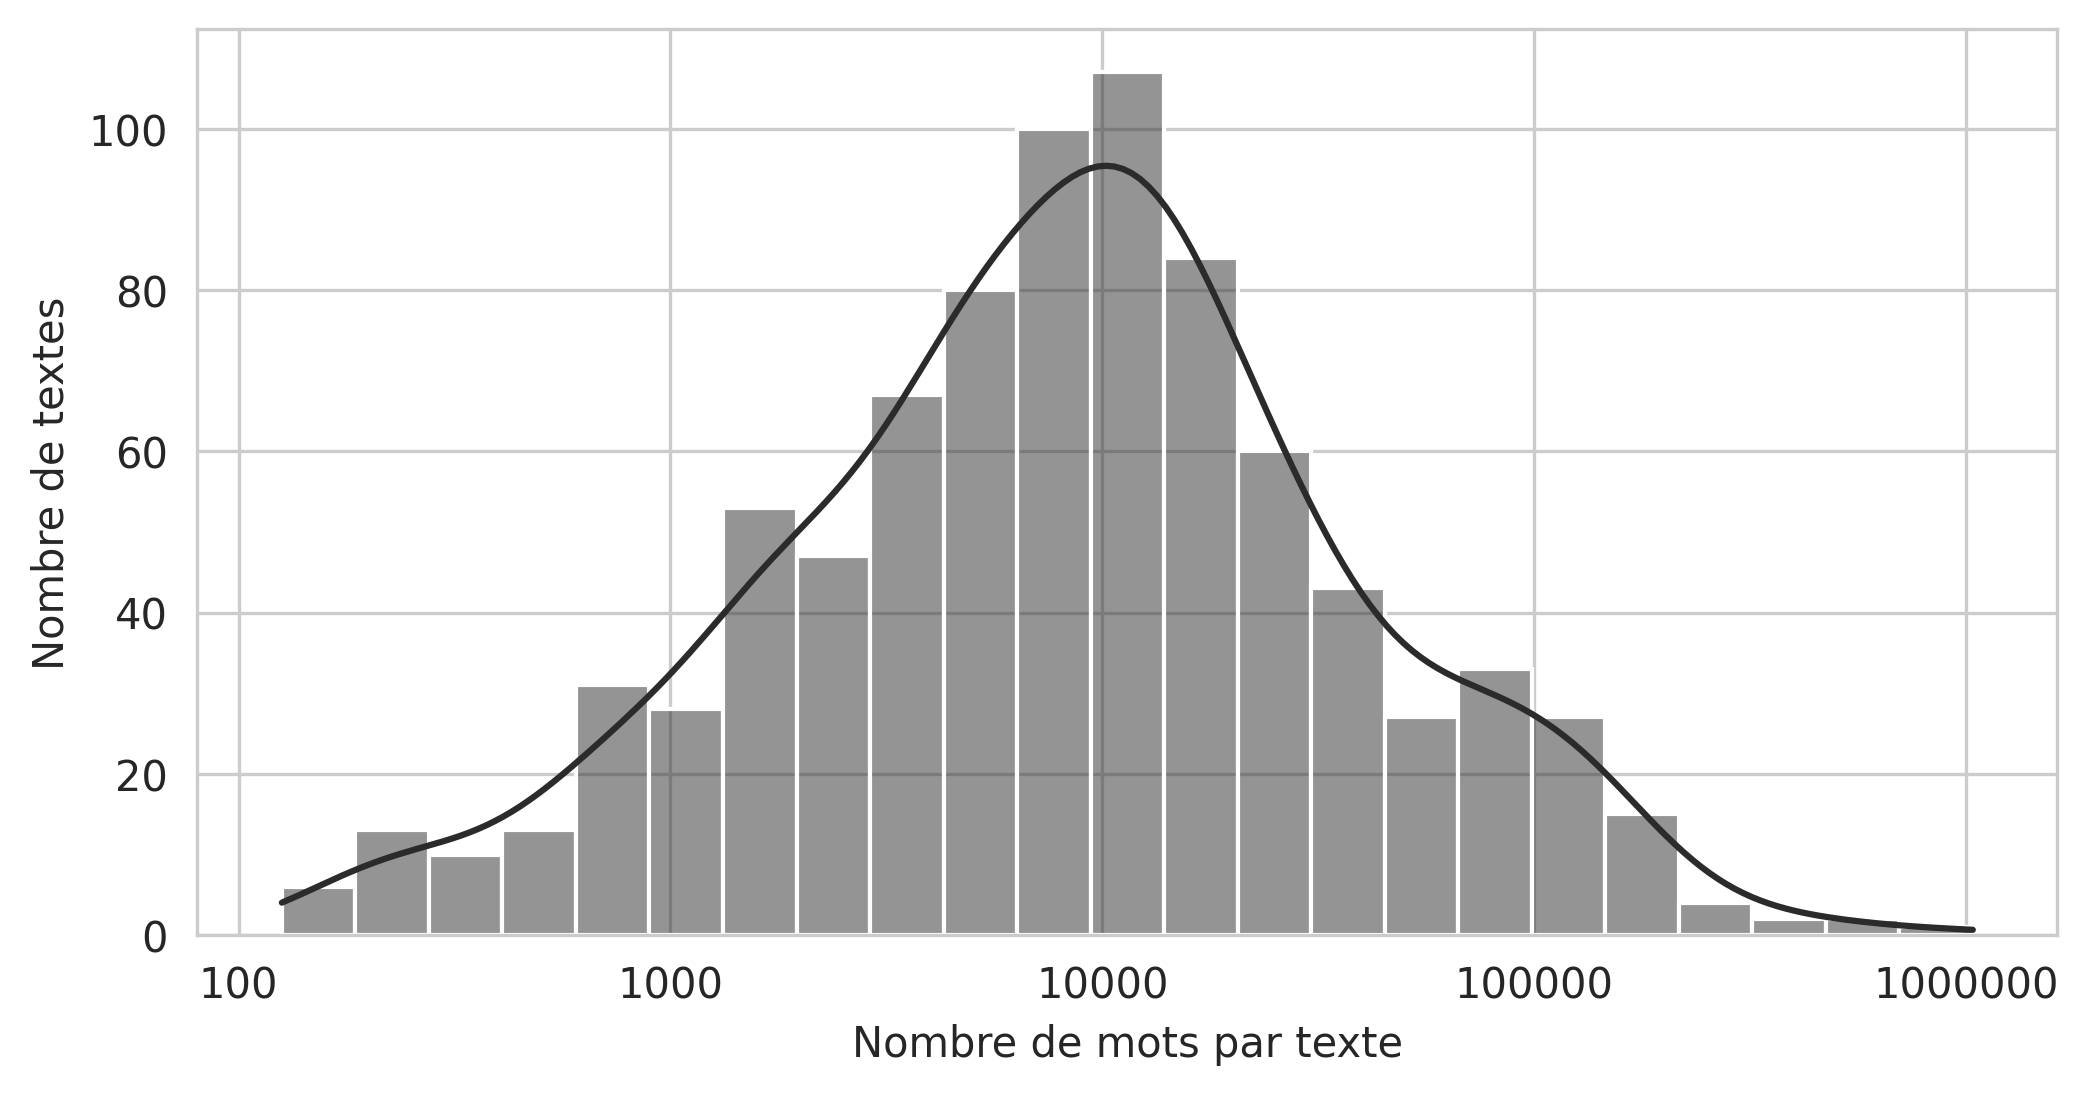
\includegraphics[width=.8\linewidth]{figures/chap1/part2/motsParTexte.png}
    \caption{Distribution des tailles de textes (en nombre de mots).}
    \label{fig:chap1:mots-par-texte}
\end{figure}
\begin{table}[]
    \centering
    \small
    \begin{tabular}{lrrrrrrrr}
    \toprule
    {} &  Oeuvres &          Moyenne &           std &    min &     25\% &     50\% &      75\% &        max \\
    \midrule
    Mots &  853 &  25003 &  59386 &  126 &  3~188 &  8~697 &  20~639 &  1~036~035 \\
    \bottomrule
    \end{tabular}
    \caption{Détails sur la répartition des tailles de textes}
    \label{tab:chap1:mots-par-textes}
\end{table}
\begin{figure}
    \centering
    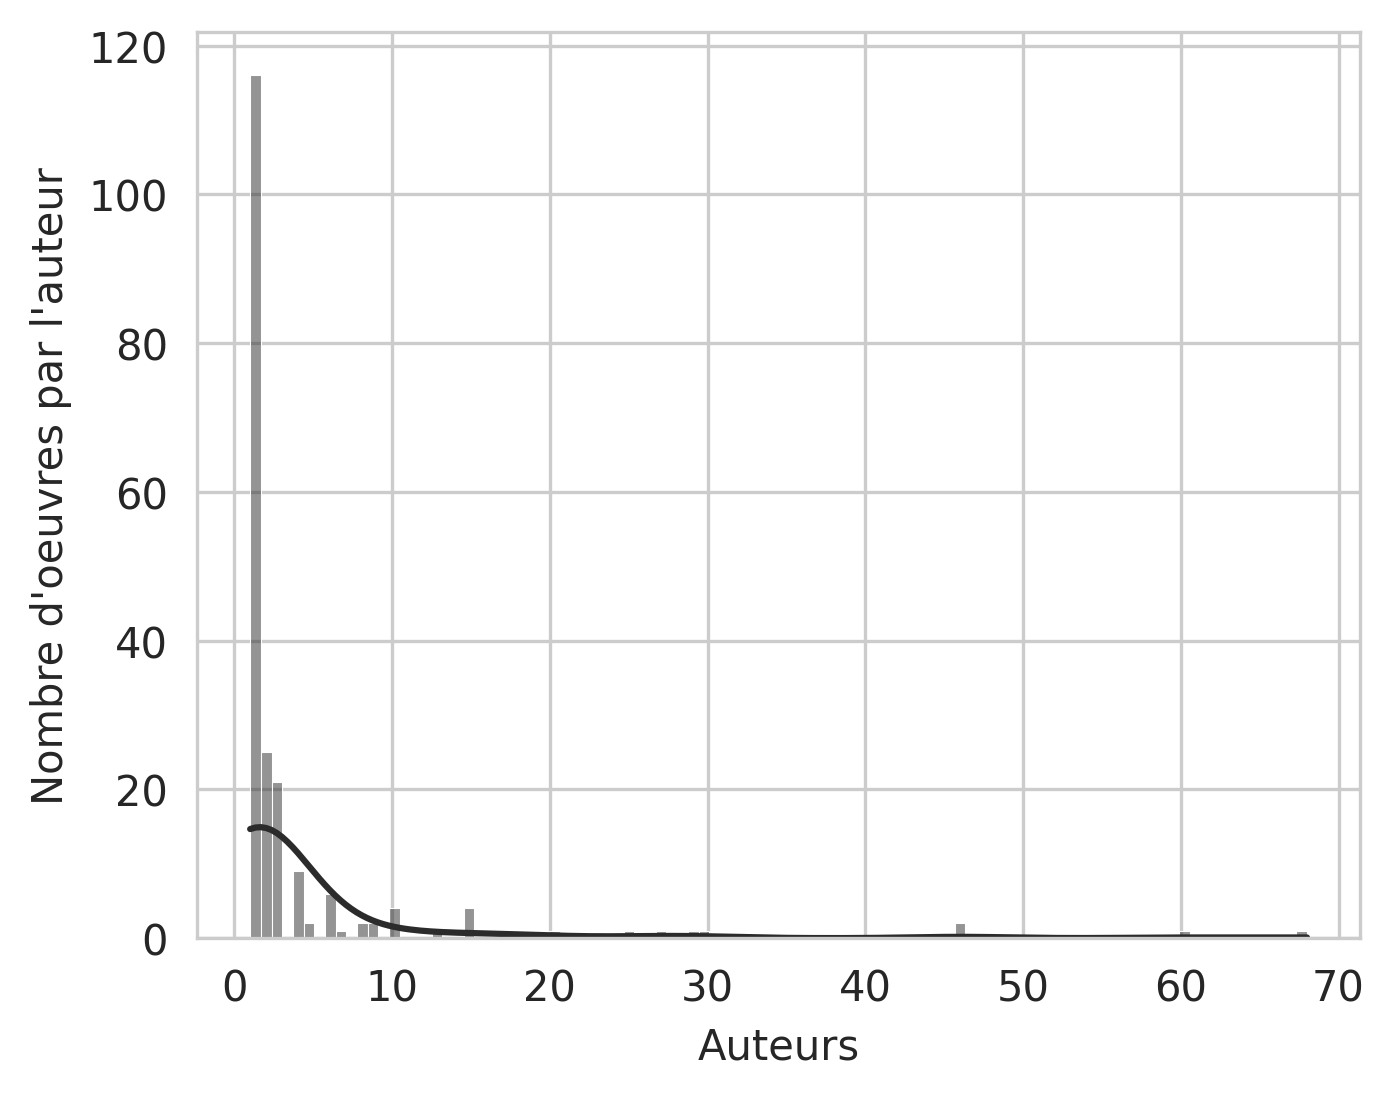
\includegraphics[height=8cm]{figures/chap1/part2/oeuvresParAuteur.png}
    \caption{Distribution du nombre d'oeuvres par auteurs. Les chiffres sont partiellement faussés par la segmentation de la bible en livres, produisant une oeuvre par livre.}
    \label{fig:chap1:oeuvres-par-auteur}
\end{figure}
\clearpage
}

\afterpage{%
\begin{sidewaysfigure}%
%\begin{figure}
    \begin{subfigure}{0.45\hsize}
        \centering
        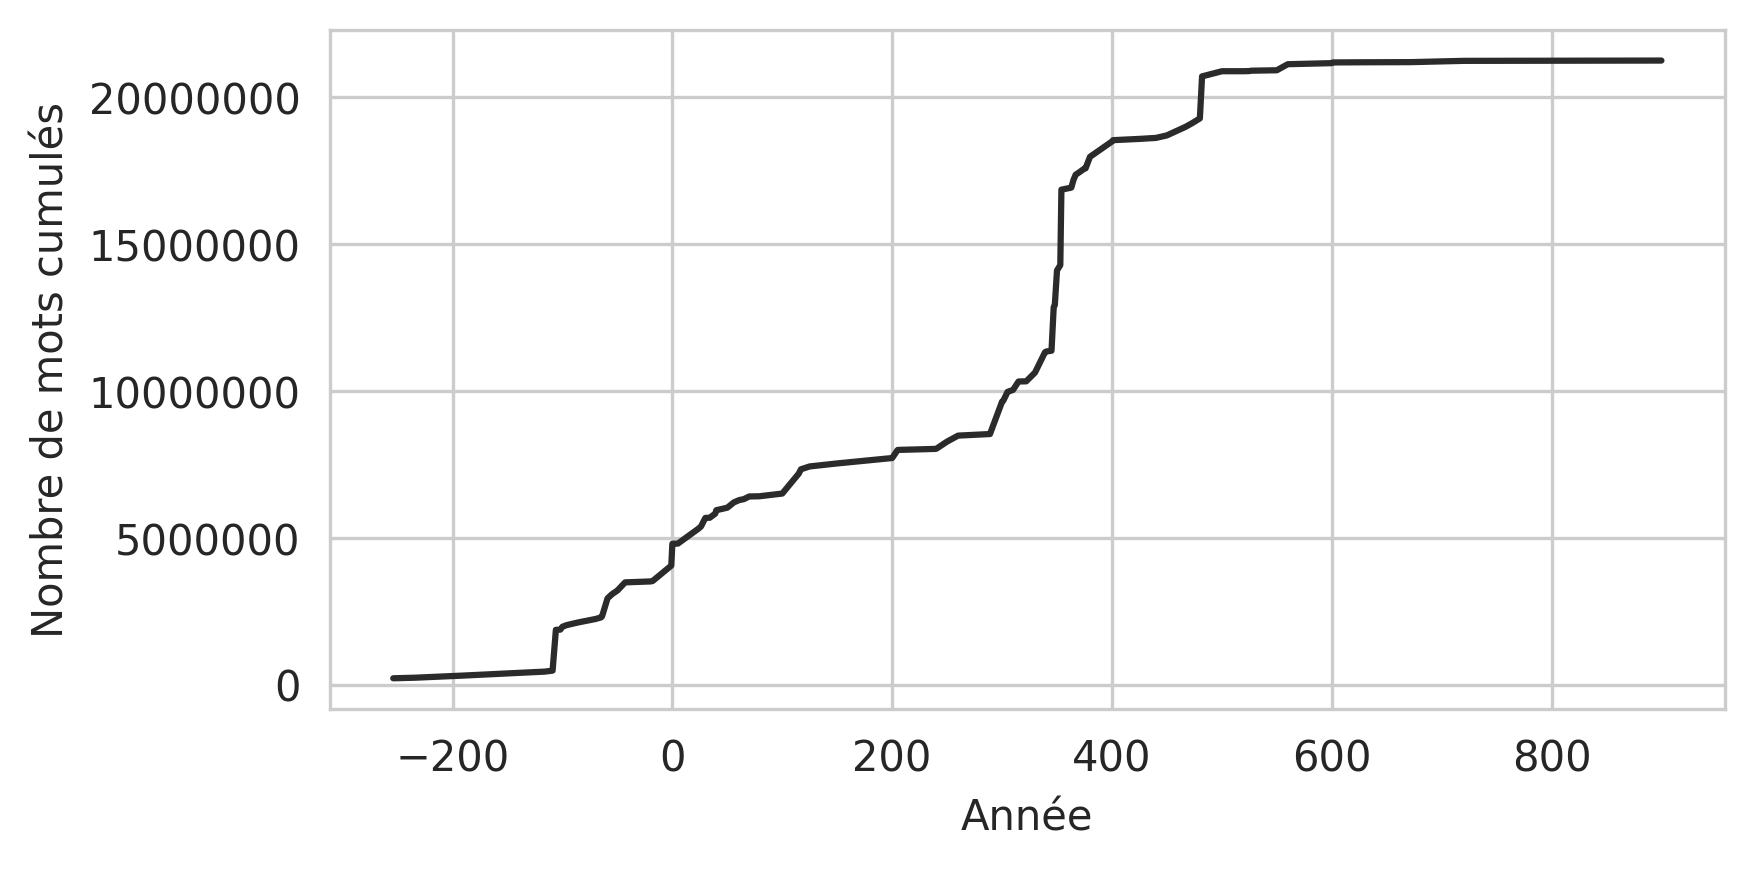
\includegraphics[width=\linewidth]{figures/chap1/part2/AccumulationMots.png}
        \caption{Accumulation générale du nombre de mots}
        \label{fig:chap1:accum-mot}
    \end{subfigure}%
    \hfill%
    \begin{subfigure}{0.45\hsize}
        \centering
        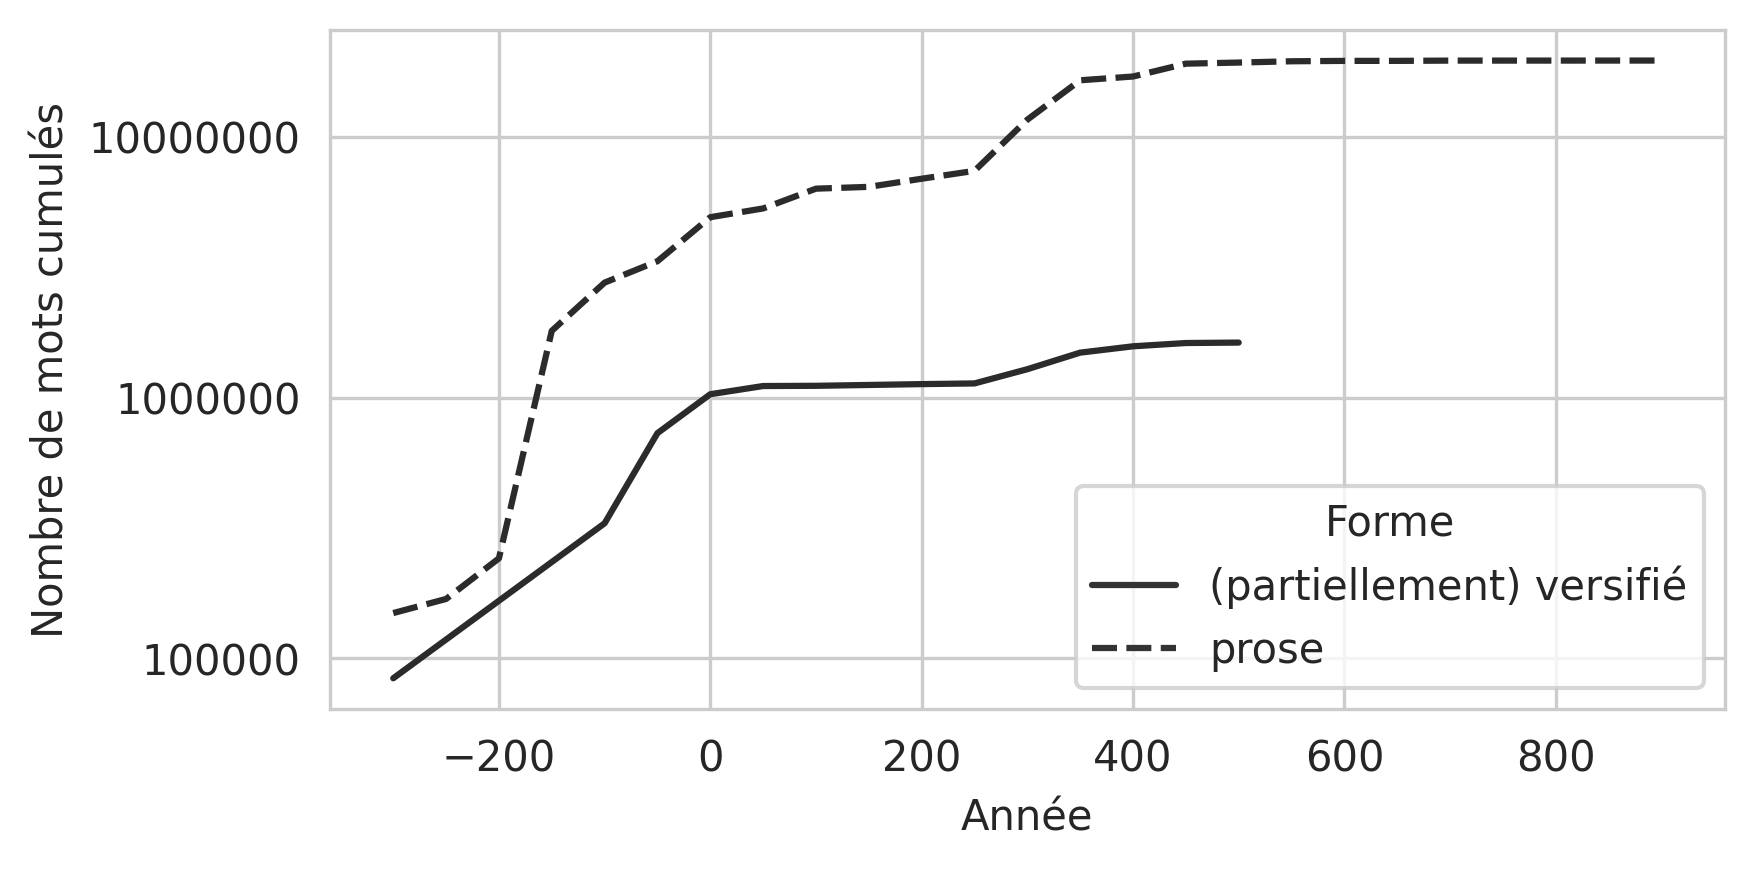
\includegraphics[width=\linewidth]{figures/chap1/part2/AccumulationMotsForme.png}
        \caption{Accumulation en fonction de la forme.}
        \label{fig:chap1:accum-mot-formes}
    \end{subfigure}%
    \vskip\baselineskip%
    \begin{subfigure}{0.45\hsize}
    \centering
    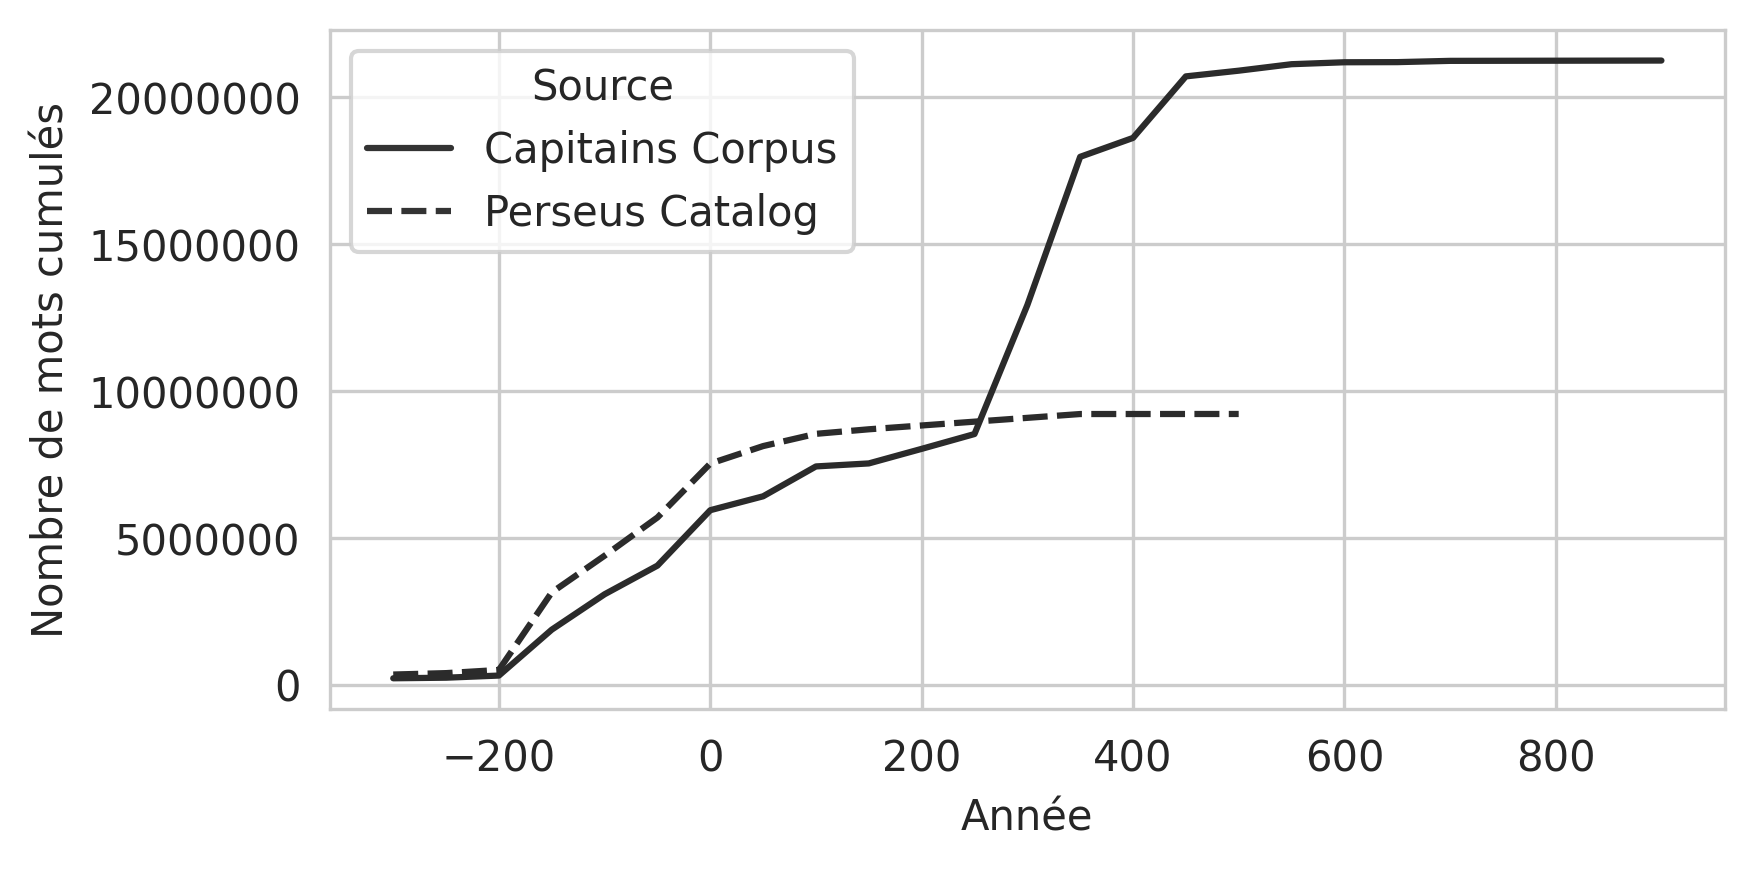
\includegraphics[width=\linewidth]{figures/chap1/part2/CatalogPerseusVSCapitains.png}
    \caption{Décompte de mots du \textit{Perseus Catalog} et de notre corpus.}
    \label{fig:chap1:accum-mot-diff-perseus-catalog}
    \end{subfigure}%
    \hfill%
    \begin{subfigure}{0.45\hsize}
        \centering
        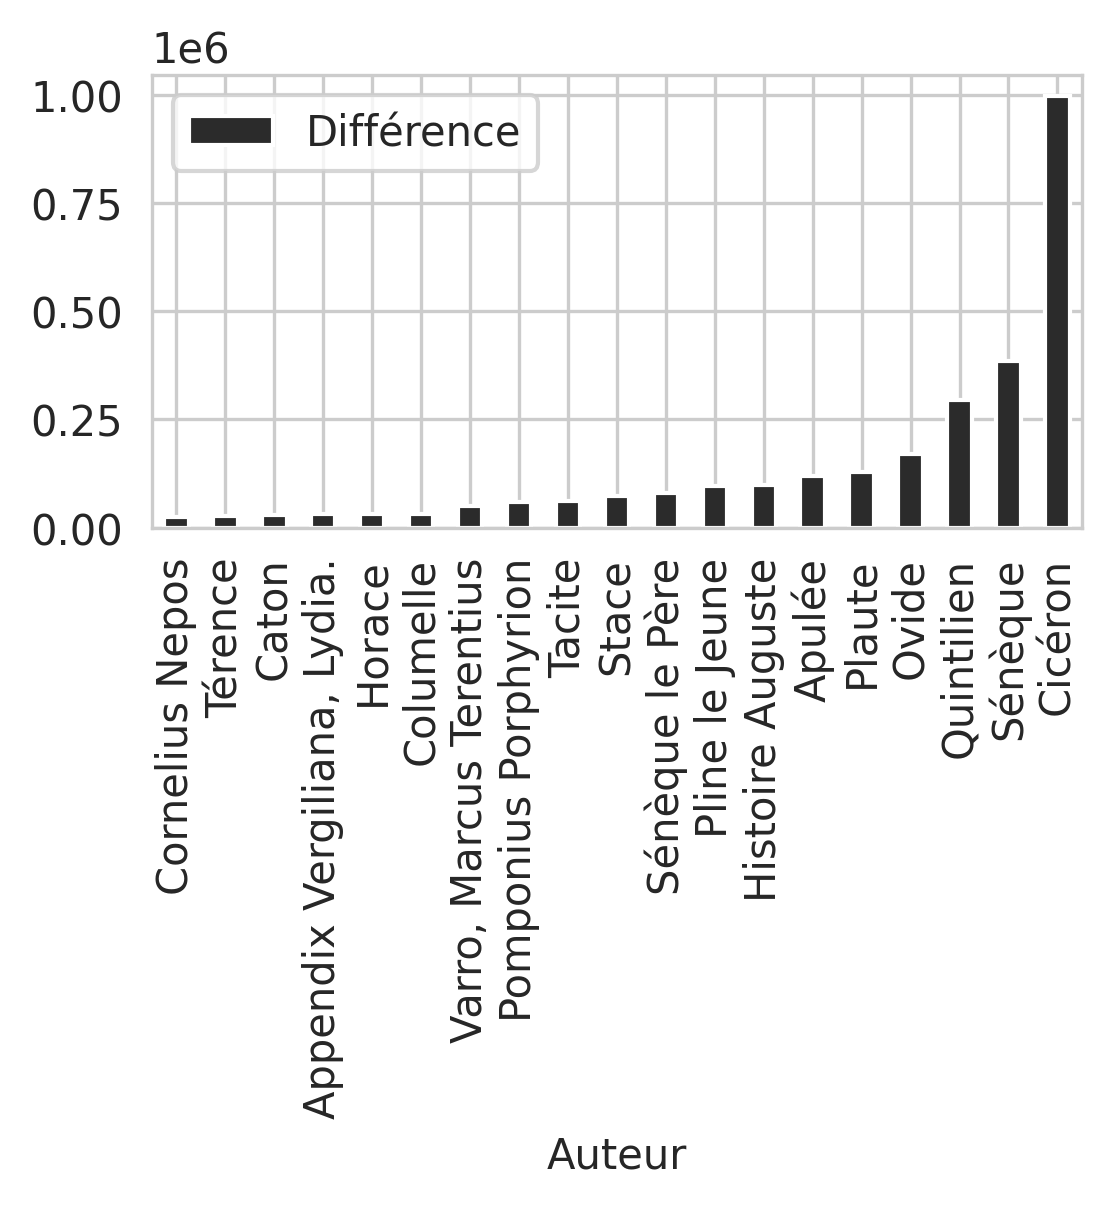
\includegraphics[width=.8\linewidth]{figures/chap1/part2/ecartsAuteurs.png}
        \caption{Écart supérieurs à 25~000 mots en défaveur de notre corpus en fonction du décompte de mots du catalogue de Perseus.}
        \label{fig:chap1:ecarts-auteurs}
    \end{subfigure}%
    \caption{Évolution de la masse du corpus. La date de composition utilisée est celle de la date de naissance présumée de l'auteur.}
\end{sidewaysfigure}%
\clearpage
}
% Le corpus final, une fois aggloméré
\clearpage

\subsection{Du corpus au document: qu’est-ce qu’un document pour l’ordinateur ?}

Nous avons vu que le corpus numérique latin, disponible dans des formats acceptables, dépasse de loin le méta-corpus accumulé ici, ne serait-ce qu'avec la \textit{Patrologia Latina} et \textit{DigilibLT}. Or, ces textes ont été laissés de côté au profit d'un corpus suivant intégralement les normes \textit{Capitains}, dont l'encodage est coûteux en temps. Nous proposons d'évaluer l'importance que peut avoir cette segmentation structurelle et son exploitabilité à travers une simple expérience: évaluer l'impact, dans une étude statistique des co-occurrents, de la prise en compte des segmentations structurelles \textit{machine actionable} de \textit{Capitains}. Dans un premier temps, nous définirons les catégories d'anlyses de cette expérience, à travers son héritage en linguistique de corpus, mais aussi à travers une définition de ce qu'est une rupture dans un \enquote{flux textuel}. Dans un second temps, nous définirons la méthode d'évaluation des corpus. Enfin, nous étudierons la différence entre les résultats des analyses effectuées\footnote{Ce texte a été réutilisé dans la publication en cours, \enquote{Thibault Clérice. \textit{"Don't worry, it's just noise": quantifying the impact of files treated as single textual units when they are really collections}}}.

\subsubsection{Concepts}

\enquote{On reconnaît un mot à ceux qui l'accompagnent.\footnote{\enquote{\textit{You shall know a word by the company it keeps }}\textcite{firth_papers_1957}}} Cette phrase de J. R. Forth, publiée en 1957, est devenue une citation classique pour définir la sémantique distributionnelle: pour trouver et comprendre le sens d'un ``mot'', on s'intéresse à ses co-occurrents.. Dans des phrases à trous telles que \enquote{Ce matin, j'ai bu un jus {[TROU]}}, il est facile de proposer des mots qui s'y retrouveraient logiquement, au premier titre desquels on aurait \enquote{d'orange}, car le contexte restreint drastiquement ce qui peut convenir après \enquote{jus}. Or, ce principe de sémantique distributionnelle est devenu si important qu'on le retrouve employé dans un très grand nombre d'outils, sans pour autant que la question de ce que forme une \enquote{compagnie} y soit remise en question\footnote{On trouve aussi le terme de \textit{voisinage} ou bien sûr de contexte en ce sens.}. Cette approche du lexique est très utilisée dans les domaines du latin et du grec ancien de la littérature classique\footcite{gillivray_greek}, tardo-antique\footcite{munson_biblical_2017}, médiévale\footcite{guerreau_pourquoi_1989,perreaux:eau} et \enquote{post-médiévale\footcite{bloem-etal-2020-distributional}} avec des corpus allant de quelques dizaines de milliers de mots à quelques millions. Mais bien souvent, les question du format des corpus et du traitement de ces format sont ignorées des descriptions des processus d'analyse, et ce qui constitue le contexte est défini majoritairement par une mesure: la fenêtre de capture de cette compagnie, c'est-à-dire le nombre de mots à gauche et à droite. 

Nous faisons l'hypothèse qu'ignorer les ruptures inhérentes aux oeuvres numérisées peut porter préjudice à la sémantique distributionnelle, d'autant plus sur des petits corpus comme le nôtre (à peine vingt millions de mots), alors que d'autres comme celui tiré de \textit{Wikipedia France} ou OSCAR (plurilingue, cent cinquante-six langues représentées) atteignent respectivement un milliard et demi et huit cents milliards\footcite{noauthor_statistiques_nodate, ortizsuarez_hal-02148693}. Parce que les oeuvres numérisées sont bien souvent des calques de la transmission papier, elles tiennent parfois plus de la collection d'oeuvres, comme les recueils d'épigrammes ou de poésie en général, que d'une oeuvre \enquote{simple}. Dans le cadre d'un commentaire d'un épigramme de Martial, il ne viendrait pas à l'idée d'un latiniste de s'appuyer sur les premiers mots de l'épigramme suivant: bien qu'il arrive qu'une unité thématique joigne quelques poèmes chez Martial, ce sont des oeuvres courtes et indépendantes les unes des autres. Or, si l'on traite un corpus de textes bruts ou de TEI sans faire attention au rôle des divisions structurelles, c'est exactement ce que la machine fait.

Nous avons vu précédemment que les oeuvres présentaient une grande variation de contenus, du discours juridique à la collection de recettes chez Apicius. Ces textes sont formés par différents niveaux de segmentation structurelle, du chapitre pour les ouvrages d'histoire par exemple aux sections pour les grands discours, en passant bien sûr par les poèmes, les livres, les recettes, etc. Ces types de contenus sont parfois introduits par la transmission des textes, parfois d'origine, mais tous décrivent -- au moins partiellement -- la relation qui lie chacune de ces unités. Il est attendu qu'une recette et une autre recette ne se retrouvent voisines que \enquote{par hasard}, ou parce qu'elles sont toutes deux des recettes de viande, tandis que deux chapitres d'un ouvrage d'histoire formeront une probable continuité narrative.

Nous souhaitons alors qualifier ces unités dans deux grandes catégories. Il y a d'une part les \enquote{unités textuelles autonomes}~(\textit{Autonomous Textual Units}, ATU): ces unités marquent une rupture avec leurs voisines. Leur contenu ne pourrait être considéré comme co-occurrents d'un point de vue lexical et sémantique: le dernier mot d'une ATU ne peut être considéré comme suivi par le premier mot de l'ATU suivante. C'est le cas d'une très grande majorité de poèmes, des définitions des \textit{Étymologies} d'Isidore de Séville, des recettes d'Apicius, des commentaires ligne à ligne de Porphyrion. D'autre part, les autres unités peuvente être qualifiées d'\enquote{unités textuelles semi-autonomes}~(\textit{Semi-autonomous textual units}, SATU): ces unités présentent des continuités narratives, thématiques ou sémantiques entre elles. C'est le cas des vers, des sections, des chapitres, etc. Par exemple, cette semi-autonomie se manifeste par la difficile lecture d'une unité sans avoir pris en compte les précédentes, ou la présence d'ellipses narratives volontaires. Continuité et ruptures sont avant tout affaire de style avant d'être des traits caractérisants des (S)ATU.

Si l'on utilise des textes sans prendre en compte leurs structures, il est probable que des unités autonomes aient leur texte compté comme co-occurrent des unités voisines. Pour évaluer ce risque, on propose de mesurer un \enquote{taux théorique de contamination des fenêtres}. Pour un texte $t$, ce taux peut être calculé en fonction du nombre de (S)ATU du texte $\left | U_{t} \right |$, de la taille de la fenêtre utilisée $W$ et enfin du nombre de mots dans le texte $\left | t \right |$ tel que

\begin{equation*}
    Taux(t) = \left \{ %
    \begin{array}{ll}
         \frac{2W(\left|U_{t}\right| - 1)}{\left|t\right|} & \quad \text{si $\left|t\right| > 2W$} \\\\
         0 & \quad \text{sinon}
    \end{array} %
    \right .
\label{equation:twcr}
\end{equation*}

\noindent où chaque mot dans une (S)ATU est contaminé par un maximum de $2W$ mots co-occurrents tirés des (S)ATU voisines, à l'exception des toutes premières et dernières (S)ATU de l'oeuvre ($\left|U\right| - 2 \times \frac{1}{2}$), qui n'ont qu'une unité voisine (d'où $\frac{1}{2}$). Ce taux représente la quantité relative de mots dont la fenêtre comporte au moins un voisin qui n'est pas censé être compté comme co-occurrent. Dans ce contexte, si l'on utilise les valeurs par défauts d'outils comme Gensim\footcite{vrehuuvrek2011gensim}, où la fenêtre est fixée à cinq ($W=5$), pour produire des analyses distributionnelles, et que l'on applique cette analyse à des oeuvres comme celle de Martial, constituée de 1527 épigrammes pour 71~911 mots, ce taux théorique est de 21,22\%. La contamination pourrait donc s'étendre jusqu'à plus d'un mot sur cinq. Au contraire, sur des textes comme le \textit{Contre Pison} de Cicéron, constitué de sections qui ne forment pas de rupture et donc dont le texte est continu, le taux de contamination sera nul.

Si le taux de contamination théorique de la fenêtre constitue un outil efficace pour considérer la question, il considère que toute (S)ATU est de longueur égale, ce qui n'est bien évidemment jamais le cas. Le taux de contamination réel dépend à la fois de la taille des trois (S)ATU à considérer: la précédente, l'actuelle et la suivante. Dans le cas de très petits poèmes comme l'\textit{Épigramme} 3.40 de Martial (10 mots), pas une seule fenêtre n’est indemne de contamination si $W=5$. Pire encore, si la fenêtre adoptée est de dix mots, soit une fenêtre tout à fait plausible, chaque mot tire des co-occurrents des deux unités voisines en même temps (\textit{cf.} Figure~\ref{exc:epigrams}).

\begin{figure}
\small
\begin{minipage}[t]{0.45\textwidth}
(Poème~39)\\*
Iliaco similem puerum, Faustine, ministro\\*
Lusca Lycoris amat. Quam bene lusca videt!\\
(Poème~40)\\*
\textit{Inserta phialae Mentoris manu} \textbf{ducta}\\*
\textit{Lacerta vivit et timetur argentum}.\\
(Poème~41)\\*
Mutua quod nobis ter quinquagena dedisti\\*
Ex opibus tantis, quas gravis arca premit,\\* {[...]}
\end{minipage} \hfill
\begin{minipage}[t]{0.45\textwidth}
(Poème~39)\\*
Iliaco similem puerum, Faustine, ministro\\*
Lusca \textit{Lycoris amat. Quam bene lusca videt}!\\
(Poème~40)\\*
\textit{Inserta phialae Mentoris manu} \textbf{ducta}\\*
\textit{Lacerta vivit et timetur argentum}.\\
(Poème~41)\\*
\textit{Mutua quod nobis ter quinquagena} dedisti\\*
Ex opibus tantis, quas gravis arca premit,\\*  {[...]}
\end{minipage}
\caption{Livre 3, poèmes 39 à 40 des \textit{Épigrammes} de Martial. Les mots considérés comme co-occurrents de \textit{ducta} pour une fenêtre de dix mots ($W=10$) sont en italique. À gauche, le résultat attendu pour un lecteur humain, prenant en compte l'absence de continuité entre les deux poèmes. À droite, la même approche, mais en prenant l'oeuvre comme une seule unité à analyser.}
\label{exc:epigrams}
\end{figure}


\subsubsection{Méthode d'évaluation}

Pour quantifier l'impact de la segmentation ou son absence, nous mettons en place toute une chaîne d'analyse permettant d'être reproduite facilement et de mettre en avant ces différences de traitement. Étant donné la particularité de l'approche -- les résultats de ces analyses ne nous intéressent pas directement, ce sont leurs différences qui sont importantes --, nous effectuons ces comparaisons à différents niveaux de traitement avec une grande variété de paramètres, souhaitant ainsi capturer plusieurs approches des textes.


\begin{figure}
    \centering
    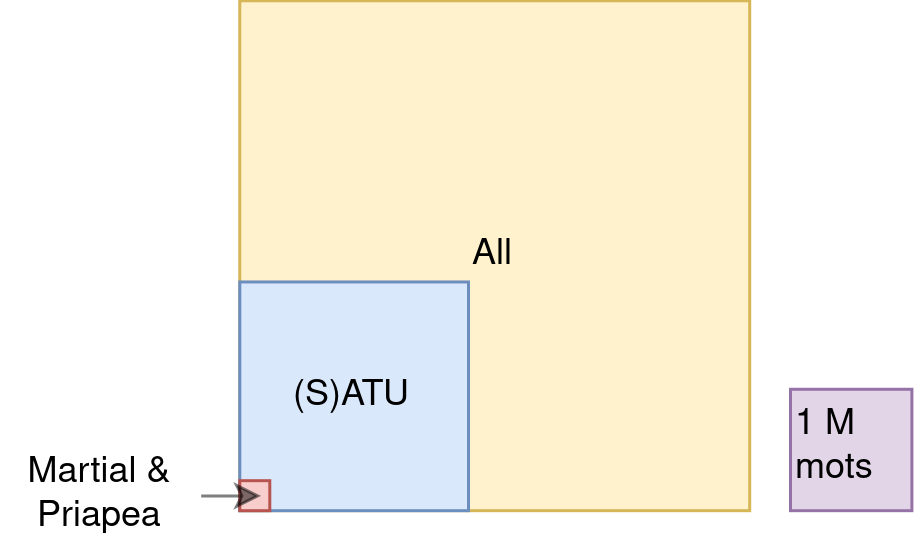
\includegraphics[width=0.6\linewidth]{figures/chap1/part2/VennCorpus.png}
    \caption{Représentation à l'échelle des trois sous-corpus et de leur relation les uns avec les autres : chaque corpus contient le ou les plus petits. }
    \label{fig:venn}
\end{figure}

Afin de quantifier l'effet de la segmentation ou de son absence, nous avons attribué à chaque texte un niveau auquel il doit être divisé, permettant ainsi de traiter les (S)ATU comme des unités non séquentielles. Pour les textes qui ne présentent pas de (S)ATU, par exemple un texte court formé de nombreux paragraphes, le texte complet a été conservé comme une seule unité. Nous produisons deux versions de chaque texte et donc de chaque corpus:
\begin{itemize}
    \item $S(T)$ (pour \textit{segment} de $T$, où $T$ est un corpus): les (S)ATU sont utilisées et les oeuvres sont découpées en autant de textes indépendants. C'est le corpus segmenté.
    \item $U(T)$ (pour \textit{*unsegment} de $T$): les (S)ATU sont ignorées et toute oeuvre présente en un seul fichier dans notre corpus est considérée comme une seule unité. C'est le corpus non segmenté.
\end{itemize}

Puis, nous divisons notre méta corpus en trois sous-corpus~(\textit{cf.} Figure~\ref{fig:venn}), représentant trois réalités différentes du point de vue des quantités, des thèmes ou encore des compositions des oeuvres qui nous ont été transmises:
\begin{enumerate}
    \item Le premier corpus ne contient que les \textit{Épigrammes} de Martial et les \textit{Priapées} (\textit{Martial \& Priapea} ci-après). Ils forment un très petit corpus ($\left | t \right |=61~082$), avec des thèmes et des lexiques communs -- ils parlent tous deux de sexualité et de manière obscène la majeure partie du temps -- et sont des textes particulièrement composites. Le premier a une structure logique en trois niveaux (livre, poème, vers), le second en seulement deux niveaux (poème, vers). Ils sont composés de poèmes qui ne forment pas de séquences narratives et donc uniquement d'ATU.
    \item Le second, \textit{Corpus ATU} ci-après, est constitué de toutes les œuvres dans lesquelles il existe un niveau de la structure logique de citation qualifié de ``poème'', ``commentaire'' ou ``scholia'', ``lettre'', ``discours'' et ``entrée'' (on trouve ces dernières pour qualifier les recettes et les niveaux des \textit{Étymologies}): cela représente 125 œuvres et 3~549~249 mots. Ils ne forment pas d'unité thématique, mais sont tout de même majoritairement composés de poésie, y compris à travers les répétions dans les \textit{scholia}. Il comprend \textit{Martial \& Priapea}.
    \item Le dernier est le méta corpus complet avec ses 17~639~626 mots (\textit{All}) .
\end{enumerate}

Chaque corpus affiche une valeur différente de la propriété combinée ``Nombre d'(ATU)-Taille du corpus'' (\textit{cf.} table \ref{tab:chap1:noise:corpora_properties}). Le premier est un très petit corpus avec un nombre élevé d'unités textuelles autonomes. Le second a un nombre élevé d'ATU, mais atteint un plus grand nombre de mots. Le dernier est un mélange massivement construit de longs passages en petite quantité par œuvre, et seuls dix pour cent de ce corpus est riche en ATU.

\begin{table*}[ht!]
    \centering
    \resizebox{1\linewidth}{!}{%
    \begin{tabular}{l|rr|rr|rr|rrrrrrr}
    \toprule
    {} & \multicolumn{2}{l}{(S)ATU} & \multicolumn{2}{l}{Mots} & \multicolumn{2}{l}{Oeuvres} & \multicolumn{7}{l}{Distribution du ratio Mots / (S)ATU} \\
    {} &  Total &     \% &     Total &     \% & Total &     \% & Moy. &  Dév. & Min & 25\% & 50\% & 75\% &    Max \\
    \midrule
    \textit{Martial \& Priapea} &   1607 &   2,8 &     61~056 &   0m3 &     2 &   0m2  &  38 &   32 &   7 &  13 &  27 &  54 &    280 \\
    Corpus ATU        &  39~591 &  68,5 &   3~549~249 &  20,1 &   125 &  14,8 &  90 &  603 &   1 &   9 &  17 &  36 &  47~783 \\
    \textit{All}               &  57~761 & 100,0 &  17~639~626 & 100,0 &   845 & 100,0 & 305 & 2~159 &   1 &  11 &  24 &  77 & 248~564 \\
    \bottomrule
    \end{tabular}%
    }
    \caption{Propriétés des différents corpus. Les signes de ponctuation sont ignorés dans le décompte des mots.}
    \label{tab:chap1:noise:corpora_properties}
\end{table*}

% Reprendre ici
% \subsubsection{Analyse sémantique et dispositif expérimental}

Comme l'objectif principal est d'analyser l'impact de la segmentation du texte sur la sémantique distributionnelle, nous mettons en place l'expérience sur la base de quatre paramètres. Nous combinons ensuite ces paramètres pour produire des analyses en utilisant les deux versions de $T$ et comparer leurs résultats. Ces quatre paramètres représentent ensemble un assez grand nombre de variations permettant de contrôler les conditions dans lesquelles $Analyse(S(T)) \neq Analyse(U(T))$: il s'agit des groupes de mots étudiés, de la taille de la fenêtre de capture des co-occurrents, des fréquences minimales pour qu'un mot soit comptabilisé dans les analyses, et enfin du nombre de groupes que l'on veut produire par \textit{clusterisation}.

Pour les groupes de mots étudiés, on utilise des termes appartenant à des champs lexicaux identifiés (famille, poésie et écriture, sexualité) afin que leur séparation en sous-groupes soit nette quand nous les regroupons. Ces groupes de mots, que nous appelons pivots, présentent aussi des particularités en termes de fréquences -- ils apparaissent tous au moins dix fois -- et de spécificités génériques:

\begin{enumerate}
    \item Le premier, \textit{Puer et al.}, contient des mots liés au foyer romain et n'est spécifique à aucun des corpus. Il s'agit de \textit{dominus, mater, pater, puella, puer, uir, uxor}, qui sont présents entre 2~036 (\textit{puella}) à 48~519 fois (\textit{dominus}) dans \textit{All}.
    \item Le second, \textit{Carmen et al.}, pourrait être plus spécifique aux grammairiens et à la poésie, qui sont surreprésentés dans \textit{Corpus ATU}. Il contient \textit{scribo, poeta, libellus, lego2, carmen1, liber1} (\textit{cf. } Table \ref{tab:chap1:noise:freq_corpora})\footnote{Lorsque les lemmes se terminent par des chiffres comme \textit{lego2}, cela représente un indice de désambiguïsation : en latin, la première personne de l'indicatif présent est souvent utilisée pour représenter le lemme, mais deux verbes partagent la forme \textit{lego} : l'un est conjugué \textit{legis} à la deuxième personne (signifiant : lire, \textit{lego2}) tandis que l'autre devient \textit{legas} (signifiant : nommer, \textit{lego1})}. 
    \item Le troisième, \textit{Puer, Carmen et al.}, est une combinaison des deux premiers et offre en tant que telle deux sous-groupes sémantiques clairement distincts qui devraient être faciles à retrouver par lexicométrie.
    \item Le dernier, \textit{Futuo, Carmen, Puer et al.}, est une combinaison des deux premiers ainsi que des mots obscènes ou du moins liés à l'expression de la sexualité : pour certains, ils sont fortement spécifiques à \textit{Martial et Priapea}, ont une fréquence très faible par rapport au premier groupe, mais sont aussi quelque peu spécifiques à \textit{Corpus ATU}. Il s'agit de \textit{cunnus, fello, futuo, irrumo, lasciuus, mentula, paedico2} (\textit{cf.} table \ref{tab:chap1:noise:freq_corpora} pour chaque fréquence de mots selon le corpus).
    \item Afin d'évaluer le bruit avant l'analyse, nous considérons également un cinquième ensemble de mots composé des 1000 mots les plus fréquents du jeu de données \textit{All}. Seuls les adverbes, adjectifs, pronoms, noms ou verbes sont pris en compte pour former ce \textit{Top 1000}.
\end{enumerate}


\begin{table}[p]
    \centering
    \begin{tabular}{l|rrr|rrrr}
    \toprule
    {} &  \makecell{Martial \\ \& Priapea} &  ATU &       All &  \makecell{Puer \\ et al.} &  \makecell{Carmen \\ et al.} &  \makecell{Puer et Carmen \\ et al.} &  \makecell{Futuo \\ et al.} \\
    \midrule
cunnus   &                  33 &              42 &        43 &         &           &                   &                        $\checkmark$ \\
fello    &                  11 &              14 &        28 &         &           &                   &                        $\checkmark$ \\
futuo    &                  46 &              52 &        52 &         &           &                   &                        $\checkmark$ \\
irrumo   &                  10 &              16 &        16 &         &           &                   &                        $\checkmark$ \\
lasciuus &                  35 &             155 &       300 &         &           &                   &                        $\checkmark$ \\
mentula  &                  68 &              75 &        75 &         &           &                   &                        $\checkmark$ \\
paedico2 &                  17 &              20 &        22 &         &           &                   &                        $\checkmark$ \\
carmen1  &                  90 &            1~753 &      3~101 &         &           $\checkmark$ &                   $\checkmark$ &                        $\checkmark$ \\
lego2    &                  95 &            3~030 &     10~252 &         &           $\checkmark$ &                   $\checkmark$ &                        $\checkmark$ \\
libellus &                 119 &             546 &      1~190 &         &           $\checkmark$ &                   $\checkmark$ &                        $\checkmark$ \\
liber1   &                  36 &            1~773 &     21~015 &         &           $\checkmark$ &                   $\checkmark$ &                        $\checkmark$ \\
poeta    &                  53 &            1~366 &      2~944 &         &           $\checkmark$ &                   $\checkmark$ &                        $\checkmark$ \\
scribo   &                  71 &            6~282 &     20~501 &         &           $\checkmark$ &                   $\checkmark$ &                        $\checkmark$ \\
dominus  &                 112 &            \textbf{7~420} &     \textbf{48~519} &         $\checkmark$ &           &                   $\checkmark$ &                        $\checkmark$ \\
mater    &                  43 &            2~132 &      9~271 &         $\checkmark$ &           &                   $\checkmark$ &                        $\checkmark$ \\
pater    &                  73 &            5~154 &     29~927 &         $\checkmark$ &           &                   $\checkmark$ &                        $\checkmark$ \\
puella   &                 120 &             989 &      2~036 &         $\checkmark$ &           &                   $\checkmark$ &                        $\checkmark$ \\
puer     &                 \textbf{159} &            1~812 &      5~824 &         $\checkmark$ &           &                   $\checkmark$ &                        $\checkmark$ \\
uir      &                  94 &            3~908 &     20~062 &         $\checkmark$ &           &                   $\checkmark$ &                        $\checkmark$ \\
uxor     &                  63 &            1~306 &      7~832 &         $\checkmark$ &           &                   $\checkmark$ &                        $\checkmark$ \\
    \bottomrule
    \end{tabular}

    \caption{Distribution des fréquences des lemmes sur les trois sous-corpus. En gras les plus hautes valeurs}
    \label{tab:chap1:noise:freq_corpora}
\end{table}


Nos deuxièmes et troisièmes paramètres sont la taille de la fenêtre, $W$, et notre seuil plancher de fréquence, $F$. $W$ varie parmi quatre valeurs ($\left [ 5, 10, 15, 20 \right ]$), capturant ainsi différentes formes de contexte: des mots immédiatement à côté de notre terme étudié à ceux dans les phrases ou ensembles syntaxiques autour de ce dernier. Pour $F$, on filtre le bruit en ne considérant que les mots qui ne sont présents qu'au moins $F$ fois dans les contextes récupérés: si \texttt{lemma1} apparaît $2$ fois avec \texttt{pivot1} et $5$ fois avec \texttt{pivot2}, il est conservé comme caractéristique si $F\geq5$. $F$ est sélectionné parmi $\left [ 1, 5, 10, 20 \right ]$: plus le nombre est haut, moins le bruit statistique sera important, les co-occurrences uniques seront ignorées lorsque $F > 1$ par exemple.


En utilisant toutes les combinaisons de $W$ et $F$ (16 combinaisons possibles par sous-corpus, soit 48 expériences), on passe les quatre premiers ensembles de mots à travers un même ensemble de traitements\footnote{\textit{Top1000} n'est pas utilisé dans toute l'expérience, voir ci-dessous.}:
\begin{enumerate}
    \item Nous récupérons la fréquence des co-occurrences dans une matrice où elles constituent des caractéristiques et où les pivots forment des classes. Cette matrice nous permet d'opérer à une première comparaison entre des décomptes bruts des $U(T)$ et $S(T)$.
    \item Suivant le travail de S. Evert\footcite{evert2005statistics}, A.~Guerreau\footcite{morsel:guerreau} et N.~Perreaux\footcite{perreaux:cbma}, nous appliquons un algorithme de normalisation appelé coefficient de \textit{Dice}. L'usage de ce coefficient permet de faire ressortir les caractéristiques les plus importantes de chaque classe.
    \item Pour chaque pivot, nous gardons leurs 5 caractéristiques les plus corrélées. Si plusieurs termes se retrouvent en cinquième place, ils sont tous considérés. Ces caractéristiques forment un deuxième ensemble de mots que nous appelons \textit{co-occurrences majeures} ($M$).
    \item Nous récupérons et augmentons la matrice originale à l'étape 1 avec la même stratégie de récupération et de stockage pour chaque mot de $M$. Les classes sont désormais formées des \textit{pivots} et de $M$.
    \item Nous normalisons à nouveau la sortie avec le coefficient de \textit{Dice}.
\end{enumerate}

C'est à ce moment de la chaîne qu'intervient notre quatrième paramètre, le nombre de groupes. La matrice normalisée finale peut être utilisée afin de produire une \textit{clusterisation}, c'est-à-dire un regroupement de classes. Nous avons utilisé un très classique \textit{clustering} agglomératif de Ward\footcite{ward1963hierarchical} à base de distances euclidiennes. Afin de pouvoir comparer les résultats du clustering sur $U(T)$ et $S(T)$, nous harmonisons les co-occurrences majeures en supprimant celles qui ne sont pas partagées entre les analyses effectuées avec les mêmes paramètres sur les deux versions de $T$. Cela produit un ensemble de classes communes $C$ qui peuvent finalement être regroupées selon un quatrième paramètre $k$, où $k$ est le nombre de \textit{clusters} que nous voulons obtenir. Nous faisons varier $k$ de sorte que $\frac{\left | C \right |}{k} < 2$ et $5 \geq k < 15$. L'étude de la variation étant l'objectif de cet article, le nombre de \textit{clusters} n'a pas besoin d'être affiné, puisque nous nous intéressons uniquement à l'égalité ou l'inégalité entre l'analyse de $U(T)$ et $S(T)$.


\subsubsection{Évaluation de l'impact}

Une fois que toutes les combinaisons et chaînes de traitement ont été exécutées, nous voulons évaluer trois différents types de différences potentielles entre les résultats de $U(T)$ et $S(T)$: un premier effet brut sur les éléments trouvés dans les contextes des groupes de mots qui forment les caractéristiques de chaque pivot, un deuxième effet sur la sélection des classes secondaires (co-occurrences majeures), impliquant donc un traitement de normalisation, et enfin l'effet sur une analyse plus avancée, le \textit{clustering}.

\paragraph{Sur la matrice de co-occurrence}
\label{chap1:noise:par:manhattan}

Pour quantifier l'impact de l'absence de segmentations structurelles sur la récupération de contexte, nous opérons d'abord à une analyse des différences assez brutes. Nous utilisons pour cela une simple distance de Manhattan entre les vecteurs de chaque pivot dans les versions segmentées et non segmentées du corpus. Ce calcul de distance est effectué pour chaque combinaison $W$ et $F$. Comme certaines caractéristiques pourraient être absentes de l'une ou l'autre des matrices, leur fréquence avec le pivot concerné est estimée à 0.

\begin{figure}[ht]
    \centering
    \begin{minipage}{.49\linewidth}%
        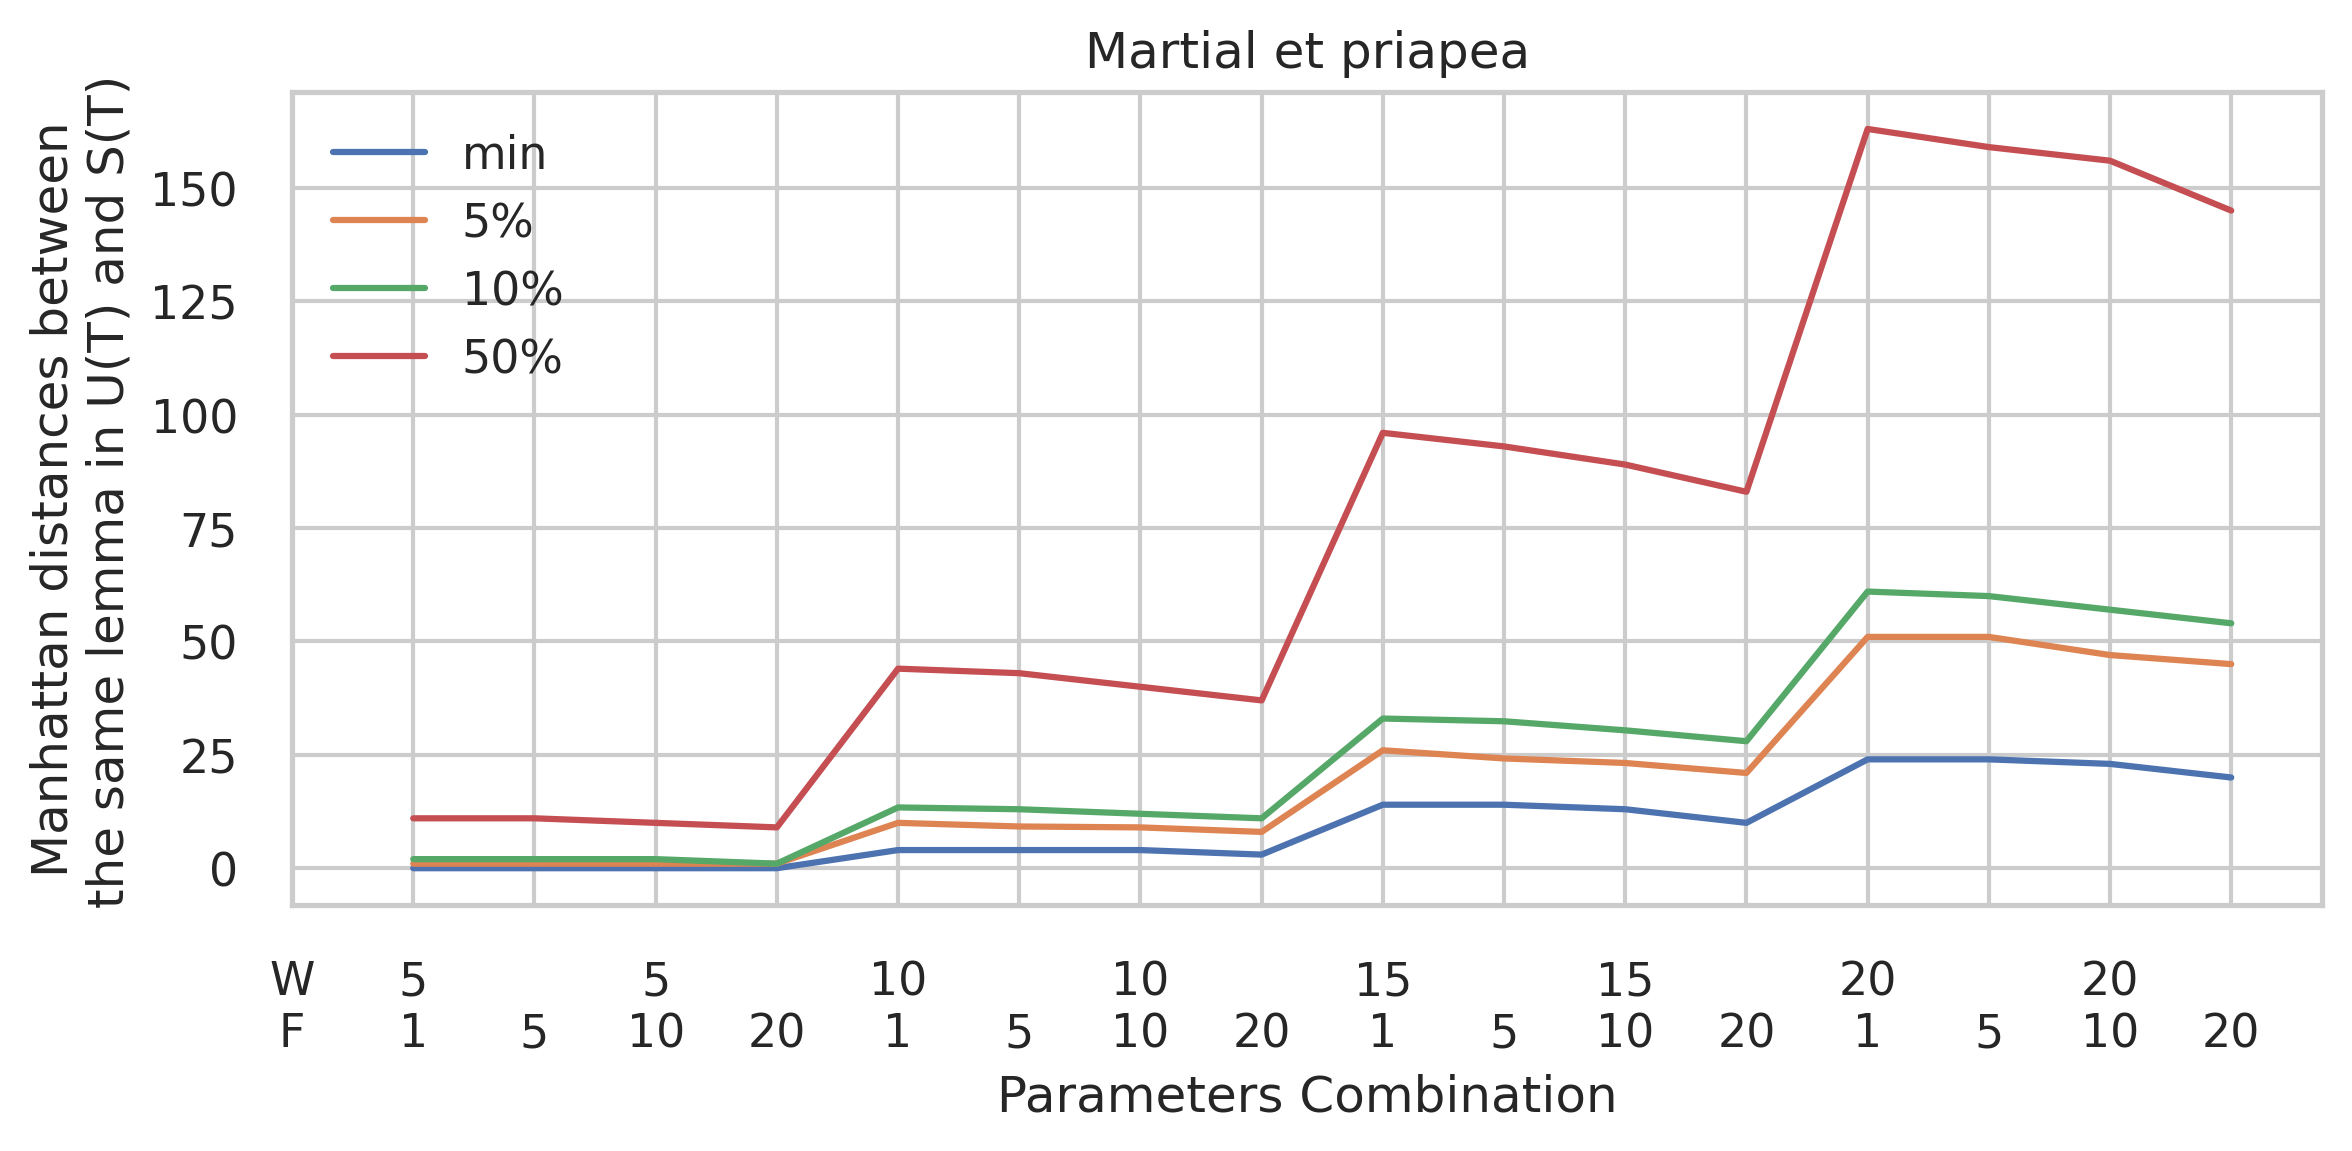
\includegraphics[width=1\linewidth]{figures/chap1/part2/manhattan_martial.png} 
    \end{minipage}%
    \hfill
    \begin{minipage}{.49\linewidth}
        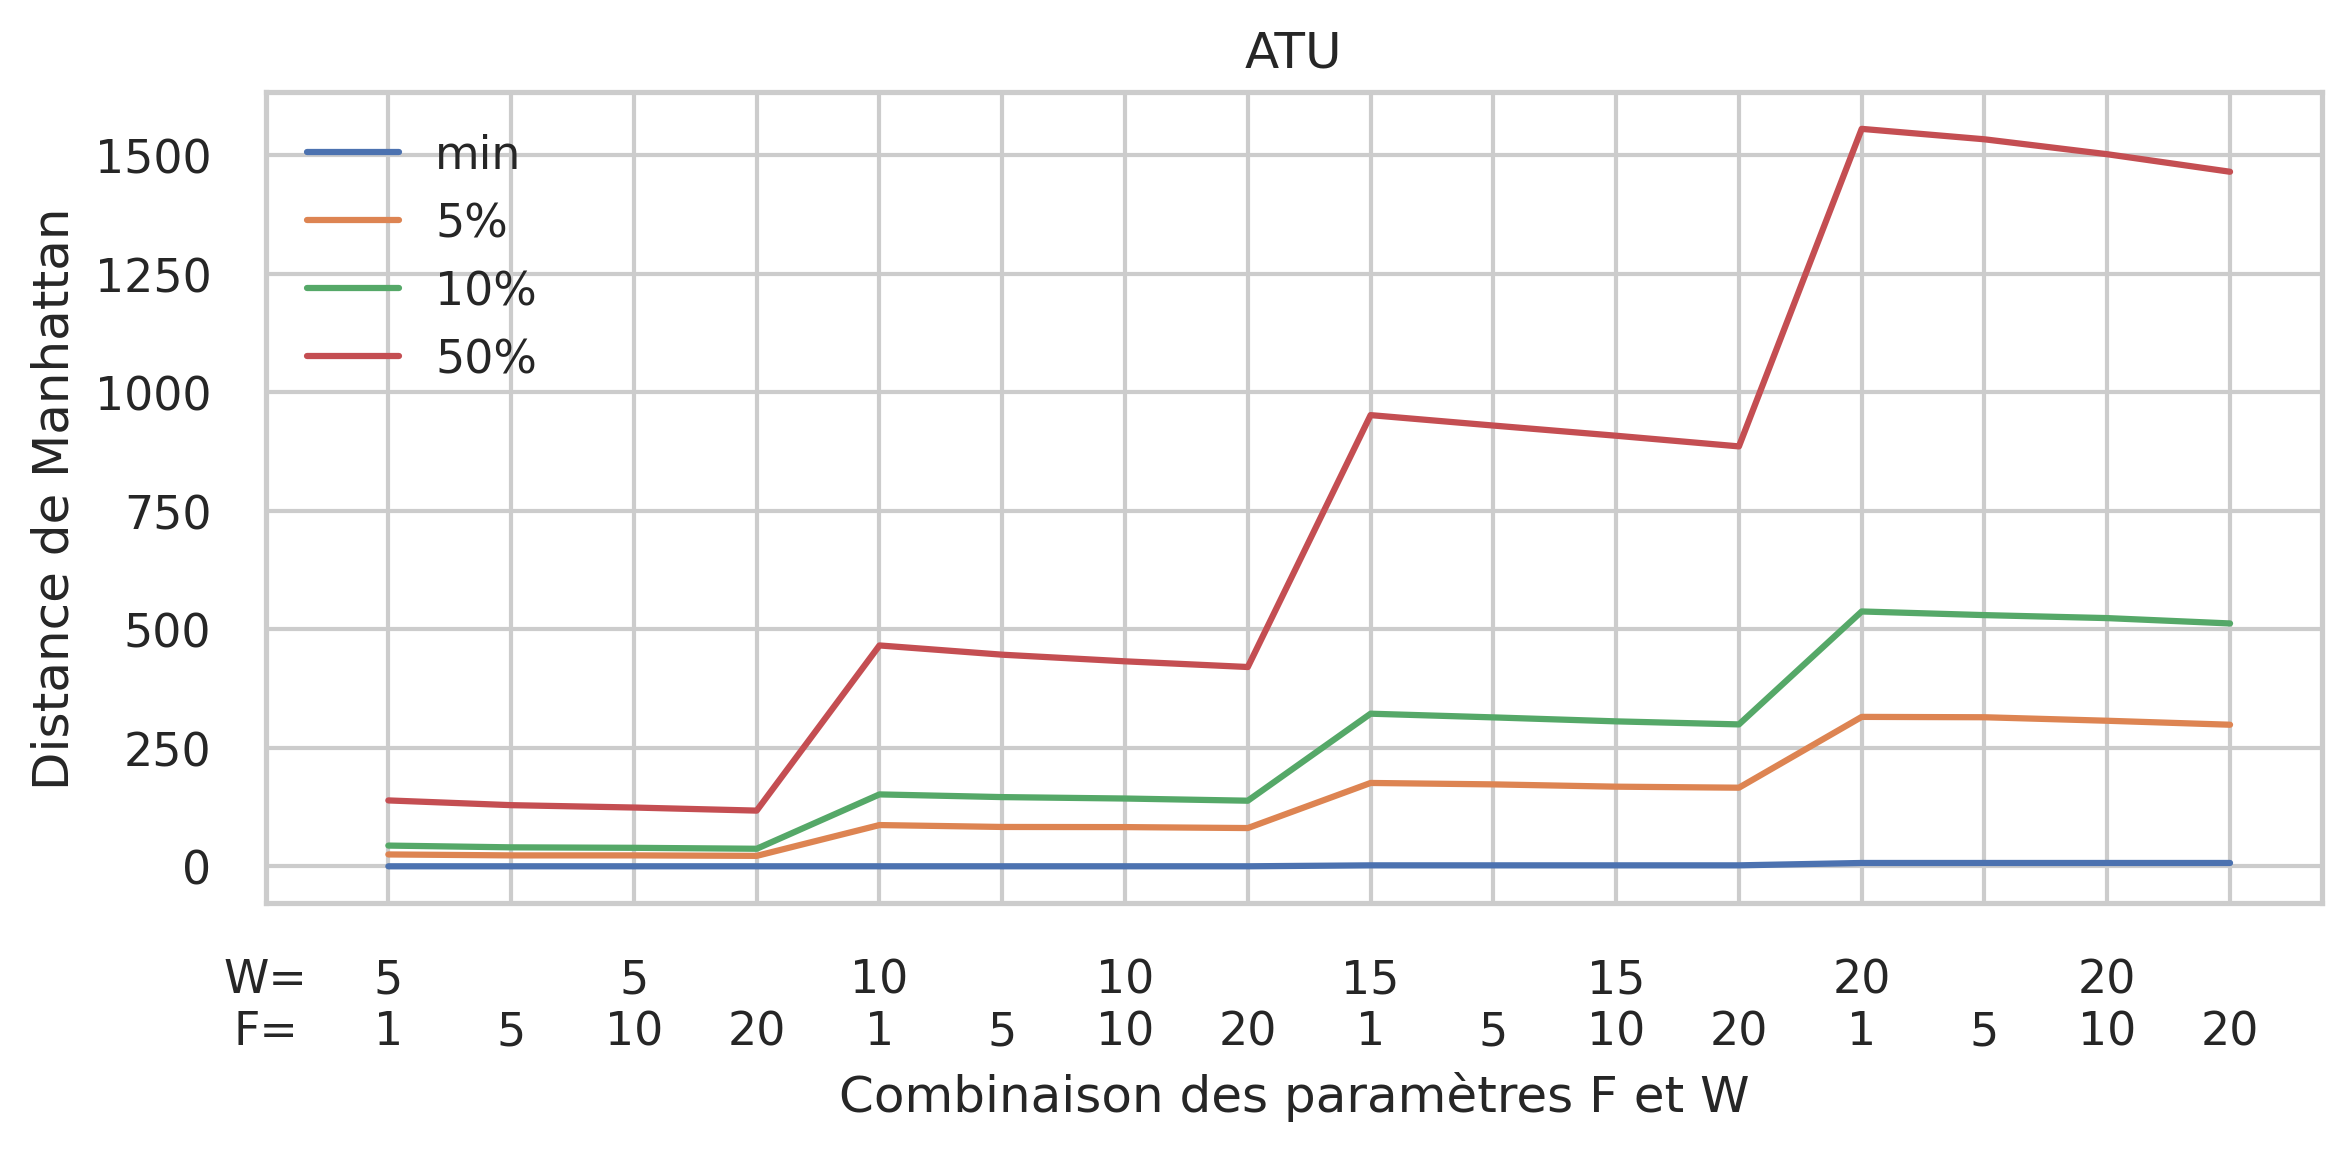
\includegraphics[width=1\linewidth]{figures/chap1/part2/manhattan_ATU.png}
    \end{minipage}
    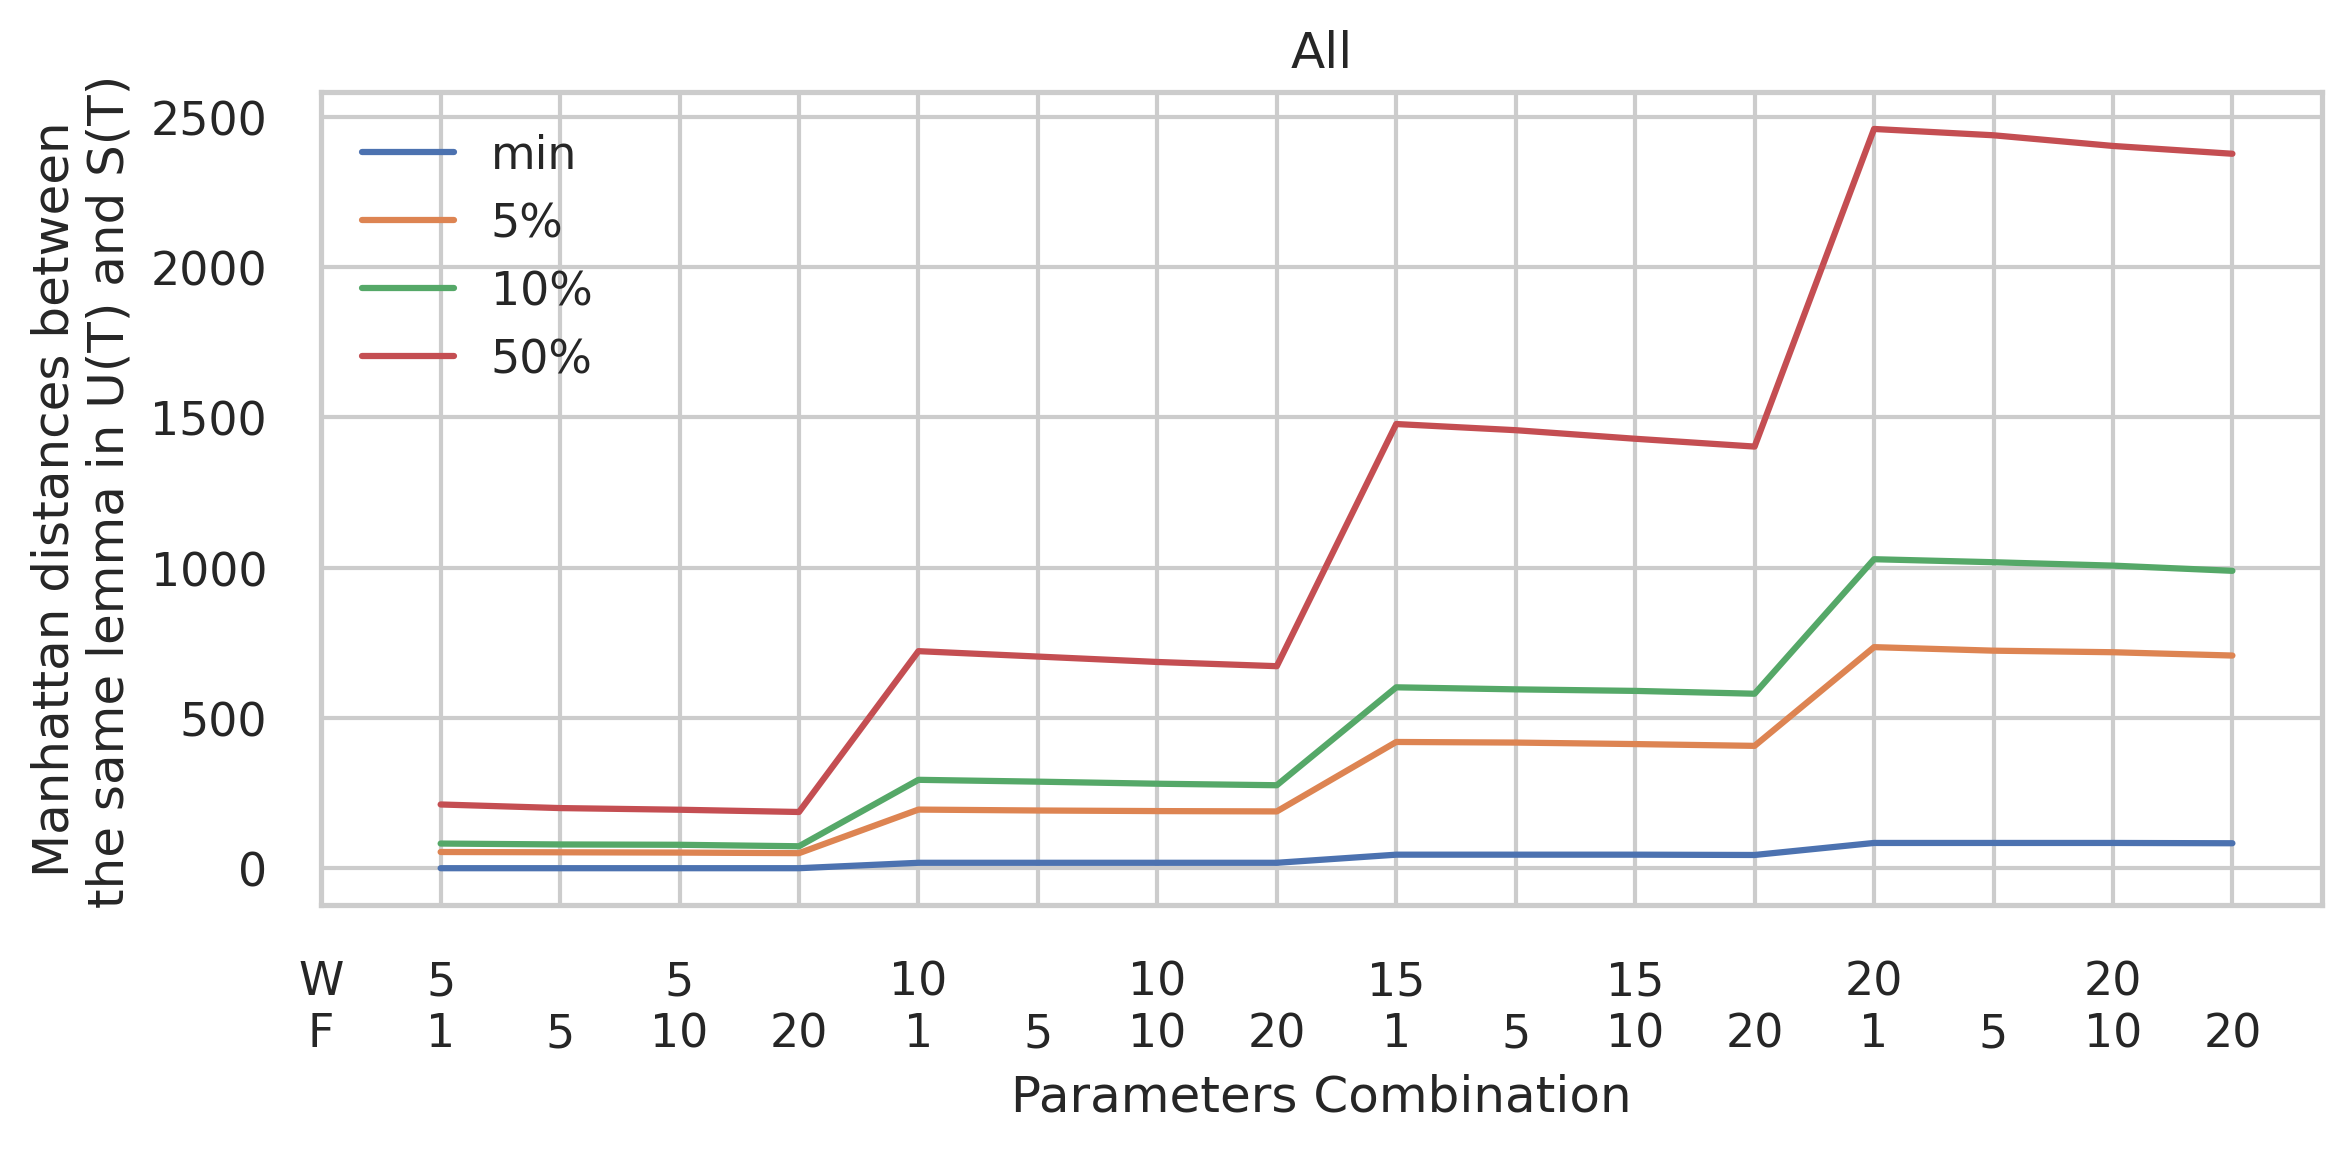
\includegraphics[width=.8\linewidth]{figures/chap1/part2/manhattan_All.png}
    \caption{Variation des percentiles (5, 10, 50) et de la valeur minimale des distances de Manhattan entre les vecteurs de chaque pivot dans $U(T)$ et $S(T)$ en fonction des valeurs de $W,F$. Résultat pour les mots les plus fréquents (\textit{Top 1000}) sur les trois sous-corpus (\textit{Martial et Priapea} en haut à gauche, \textit{ATU} en haut à droite, \textit{All} en bas).}
    \label{fig:chap1:noise:manhattan}
\end{figure}

On distingue nettement trois effets dans résultats (\textit{cf.} figure \ref{fig:chap1:noise:manhattan}):
\begin{itemize}
    \item Quelle que soit la fenêtre $W$, le seuil $F$ a un effet très limité. Ce filtrage croît -- même minimalement -- en même temps que sa valeur: plus il est grand, plus il réduit la distance mesurée.
    \item Le changement de la taille de la fenêtre $W$ a un impact important sur les distances intervecteur, ce qui est attendu: plus le contexte relevé est grand, plus il est probable que ce contexte \enquote{pioche} dans des unités voisines, mais indépendantes.
    \item Tous les sous-corpus sont touchés, mais tous les mots ne sont pas touchés autant. À partir du corpus \textit{ATU}, certains mots sont très peu touchés voir indemnes de toute contamination. Cependant, on aperçoit dès le percentile 5\% des variations de plus en plus importantes en fonction de $W$.
\end{itemize}

Du point de vue de la collecte brute donc, il est clair qu'une différence existe entre $S(T)$ et $U(T)$.

\paragraph{Sur les classes}
\label{sub:major-co-occurrences}

Sur la base de cette première observation, nous voulons évaluer ce que ce bruit peut faire à des sélections de caractéristiques plus avancées. Chez Guerreau et Perreaux, le coefficient de Dice est utilisé pour trouver des termes \textit{affiliés} aux termes qu'ils veulent étudier pour les placer dans des réseaux plus grands. En appliquant ce coefficient et en sélectionnant les termes les plus proches, on peut alors comparer les co-occurrents majeurs sélectionnés ($M$) dans $U(T)$ et $S(T)$. Compte tenu des différences de distances constatées ci-dessus, on cherche donc à vérifier si ces dernières sont à même d'être gommées par une normalisation. 

\begin{figure}[h]
    \centering
    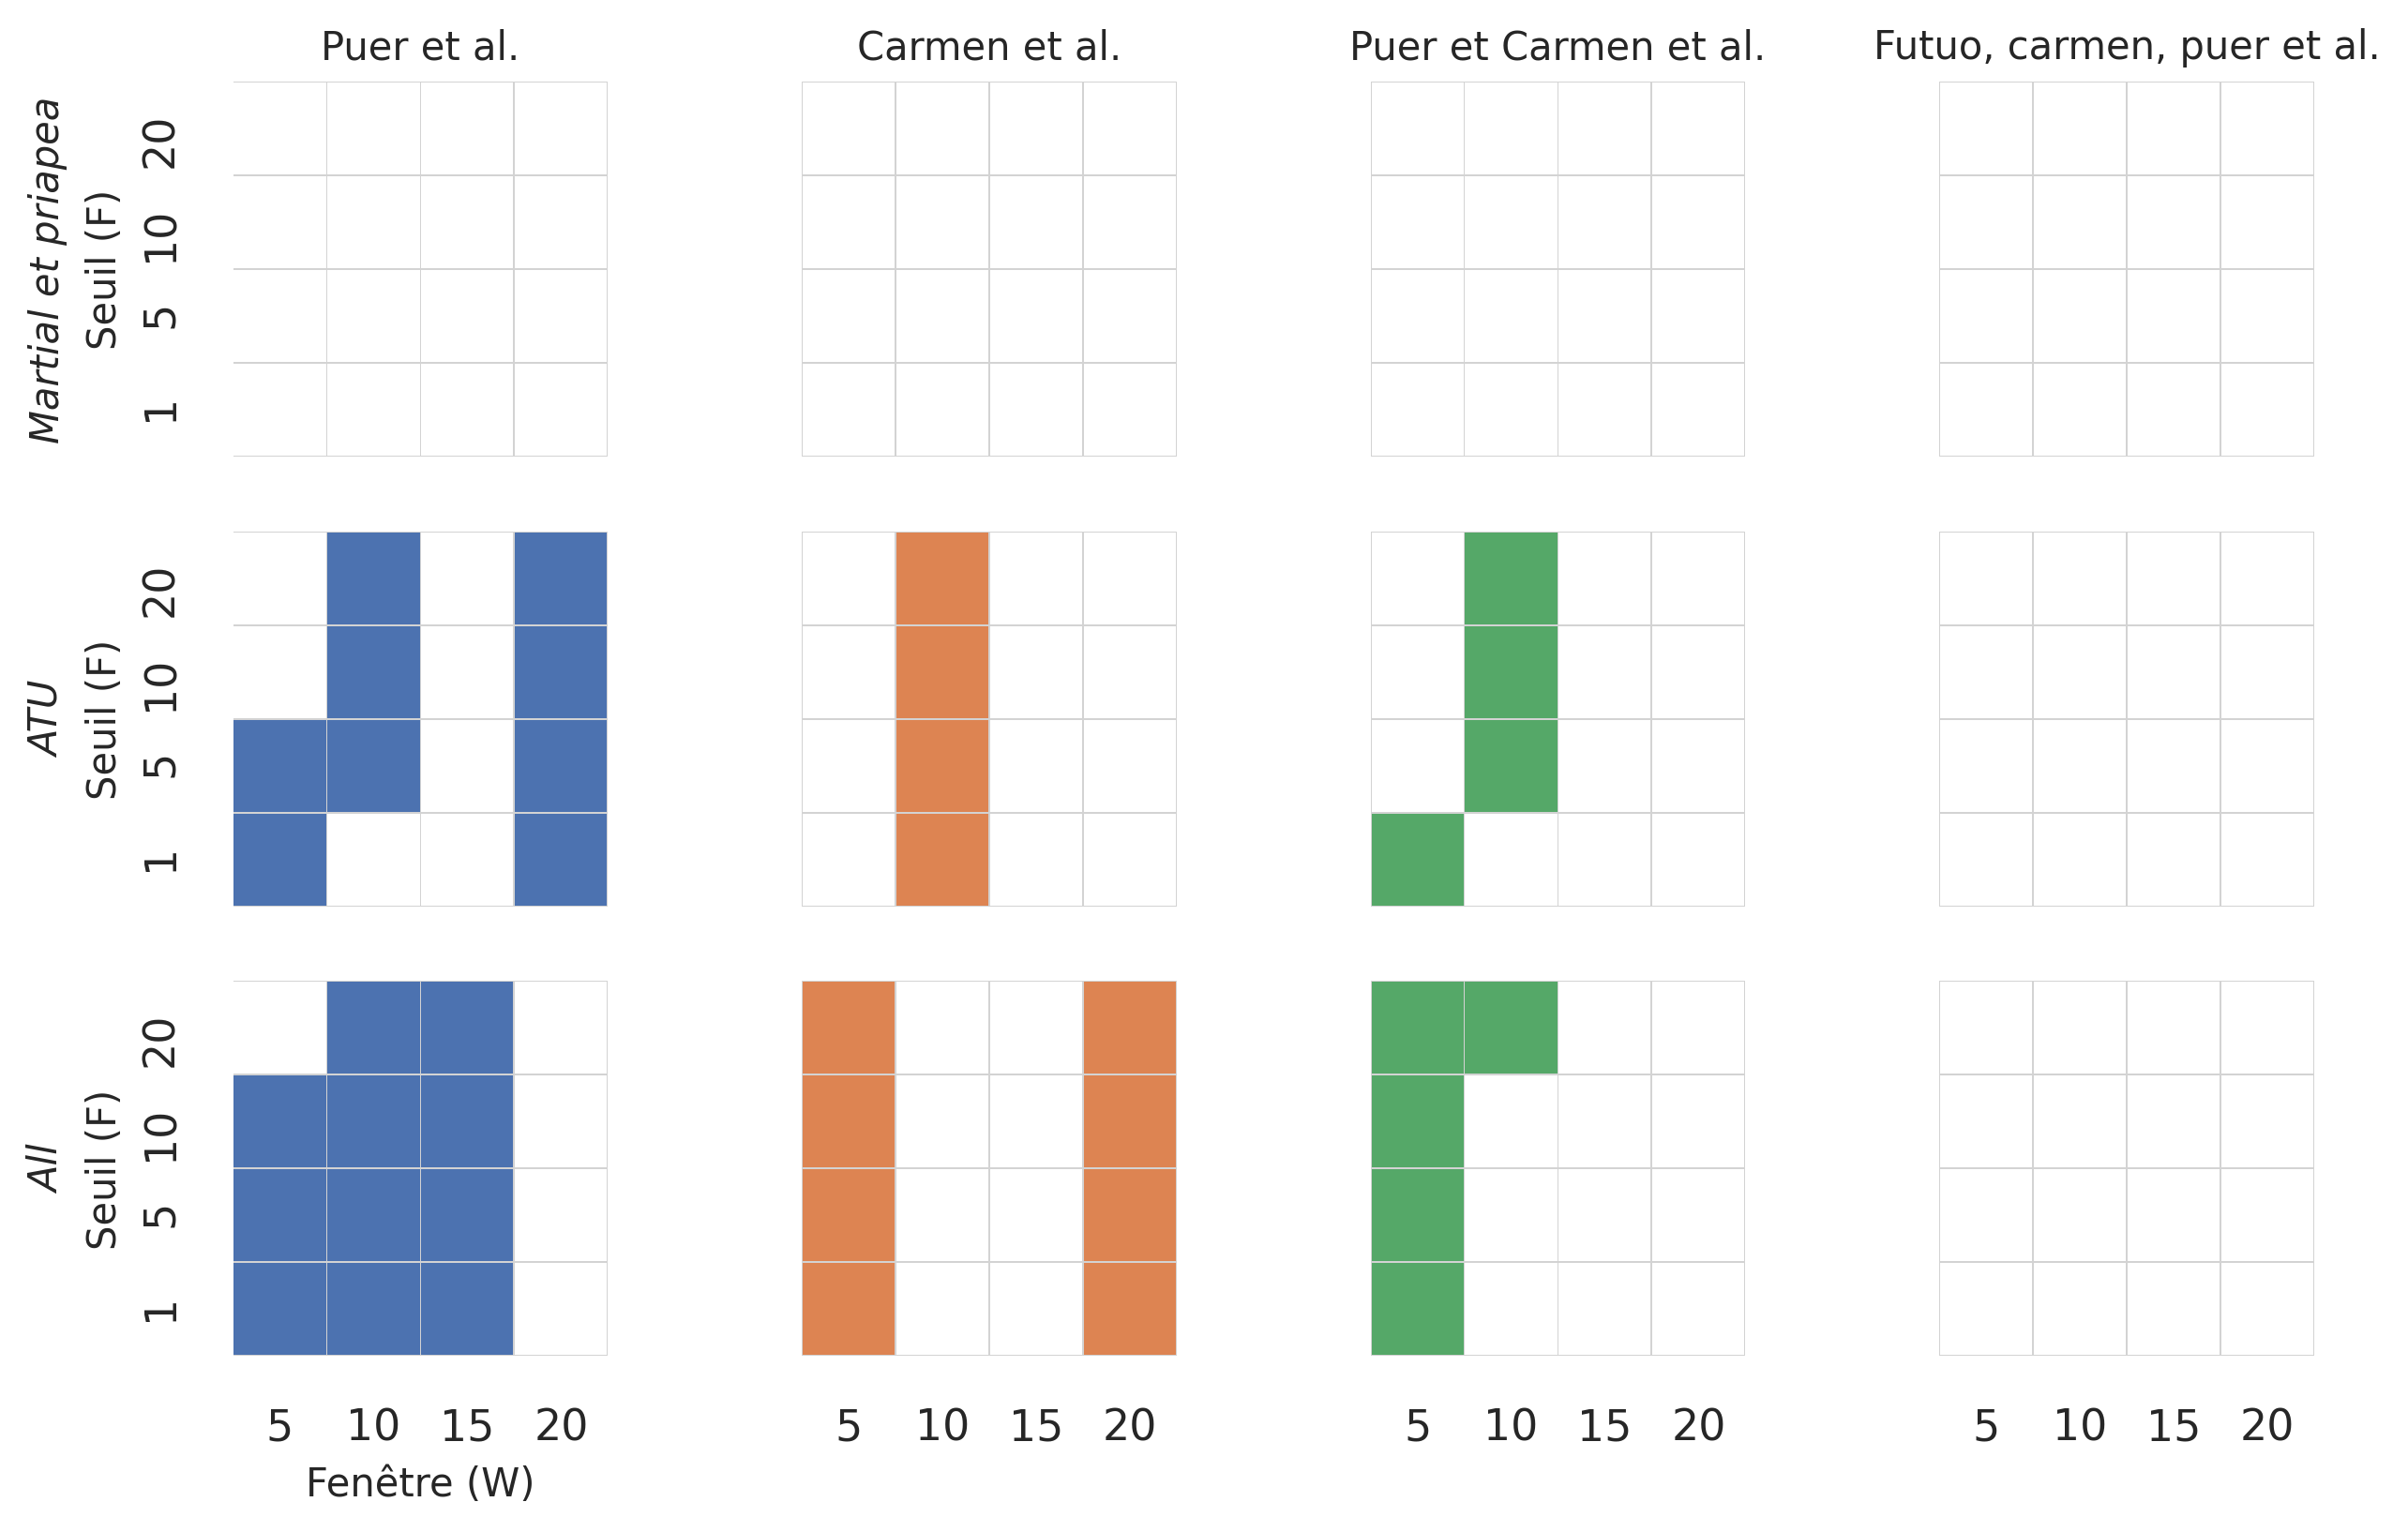
\includegraphics[width=.95\linewidth]{figures/chap1/part2/classes_binary.png}
    \caption{Matrice binaire de $M_{S(T)} = M_{U(T)}$ : les cellules colorées signifient que l'analyse des deux versions du corpus avec les mêmes paramètres a donné lieu aux mêmes co-occurrences majeures.}
    \label{fig:chap1:noise:matrix_classes}
\end{figure}


 Nous quantifions d'abord cet effet par une approche binaire, c'est-à-dire que nous vérifions que $M_{S(T)}$ et $M_{U(T)}$ sont strictement égaux. Toute situation où $M_{U(T)} \neq M_{S(T)}$ est une autre preuve que l'absence de segmentation a un impact. Or, seuls 21,35\% (41/192) des expériences et combinaisons de paramètres et données étudiées (Mots, Fenêtre, Seuil, Corpus) produisent une sélection de co-occurrents majeurs parfaitement égaux pour les deux versions de $T$, avec des résultats variables selon le groupe de mots et le corpus (\textit{cf.} Figure~\ref{fig:chap1:noise:matrix_classes}) :
 
% [2/1/22] RÉDACTION REPRENDRE ICI

 \begin{itemize}
    \item Le groupe de mots ``\textit{Futuo et al.}'' ne donne jamais lieu à des $M$ identiques entre $S(T)$ et $U(T)$. Il s'agit du seul groupe de mots ne formant jamais d'identité entre les deux versions du corpus: il est caractérisé par des fréquences plus basses que les autres groupes -- à travers \textit{irrumo} par exemple -- et est donc plus touché par le bruit dû à l'absence de segmentation.
    \item Tout comme ``\textit{Futuo et al.}'', le corpus \textit{Martial \& Priapea} -- le plus petit et le plus riche en ATU -- est fortement affecté par la différence de traitement des textes: aucune analyse ne produit de $M$ identiques, le bruit n'est pas atténué par la normalisation.
    \item Le groupe ``Puer et al.'' atteint majoritairement une égalité de résultat sur le corpus \textit{ATU Corpus} (neuf combinaisons sur seize), mais cette attitude est inconstante en regard de $W$ et $F$. Cela plaide simplement en faveur d'une segmentation des corpus (S)ATU riches comme préalable à une analyse similaire à celle que nous menons ici. La fréquence ``plutôt faible'' de \textit{libellus}~(546) dans le \textit{Carmen et al.} et le \textit{Puer et Carmen et al.} pourrait être responsable d'une partie de l'instabilité, bien qu'elle soit bien au-dessus de la fréquence de l'ensemble des termes  de la sexualité.
    \item La taille des corpus lisse le bruit des caractéristiques, car le corpus \textit{All} affiche une plus grande stabilité entre $M_{S(T)}$ et $M_{U(T)}$, en particulier pour \textit{Puer et al.}, mais les $M$ restent plus souvent inégaux qu'égaux.
    \item Le seuil de fréquence des co-occurrences $F$ a un impact très faible sur les co-occurrences majeures, comme vu précédemment pour \textit{Top 1000}, tandis que la fenêtre affecte irrégulièrement les ensembles de mots. À titre d'exemple, $W=15$ ne produit jamais de résultats identiques entre $S(T)$ et $U(T)$ pour la combinaison \textit{Carmen et al. }~+~\textit{All} (orange, en bas), mais elle le fait pour  \textit{Puer et al.} (bleu, en bas); au contraire, $W=15$ échoue sur \textit{Puer et al.}~+~\textit{ATU}. Cette instabilité de l'impact de $W$ plaide également en faveur de l'utilisation de (S)ATU lors d'une telle analyse.
\end{itemize}

\begin{figure}[h]
    \begin{minipage}[t]{.55\linewidth}
        \centering
        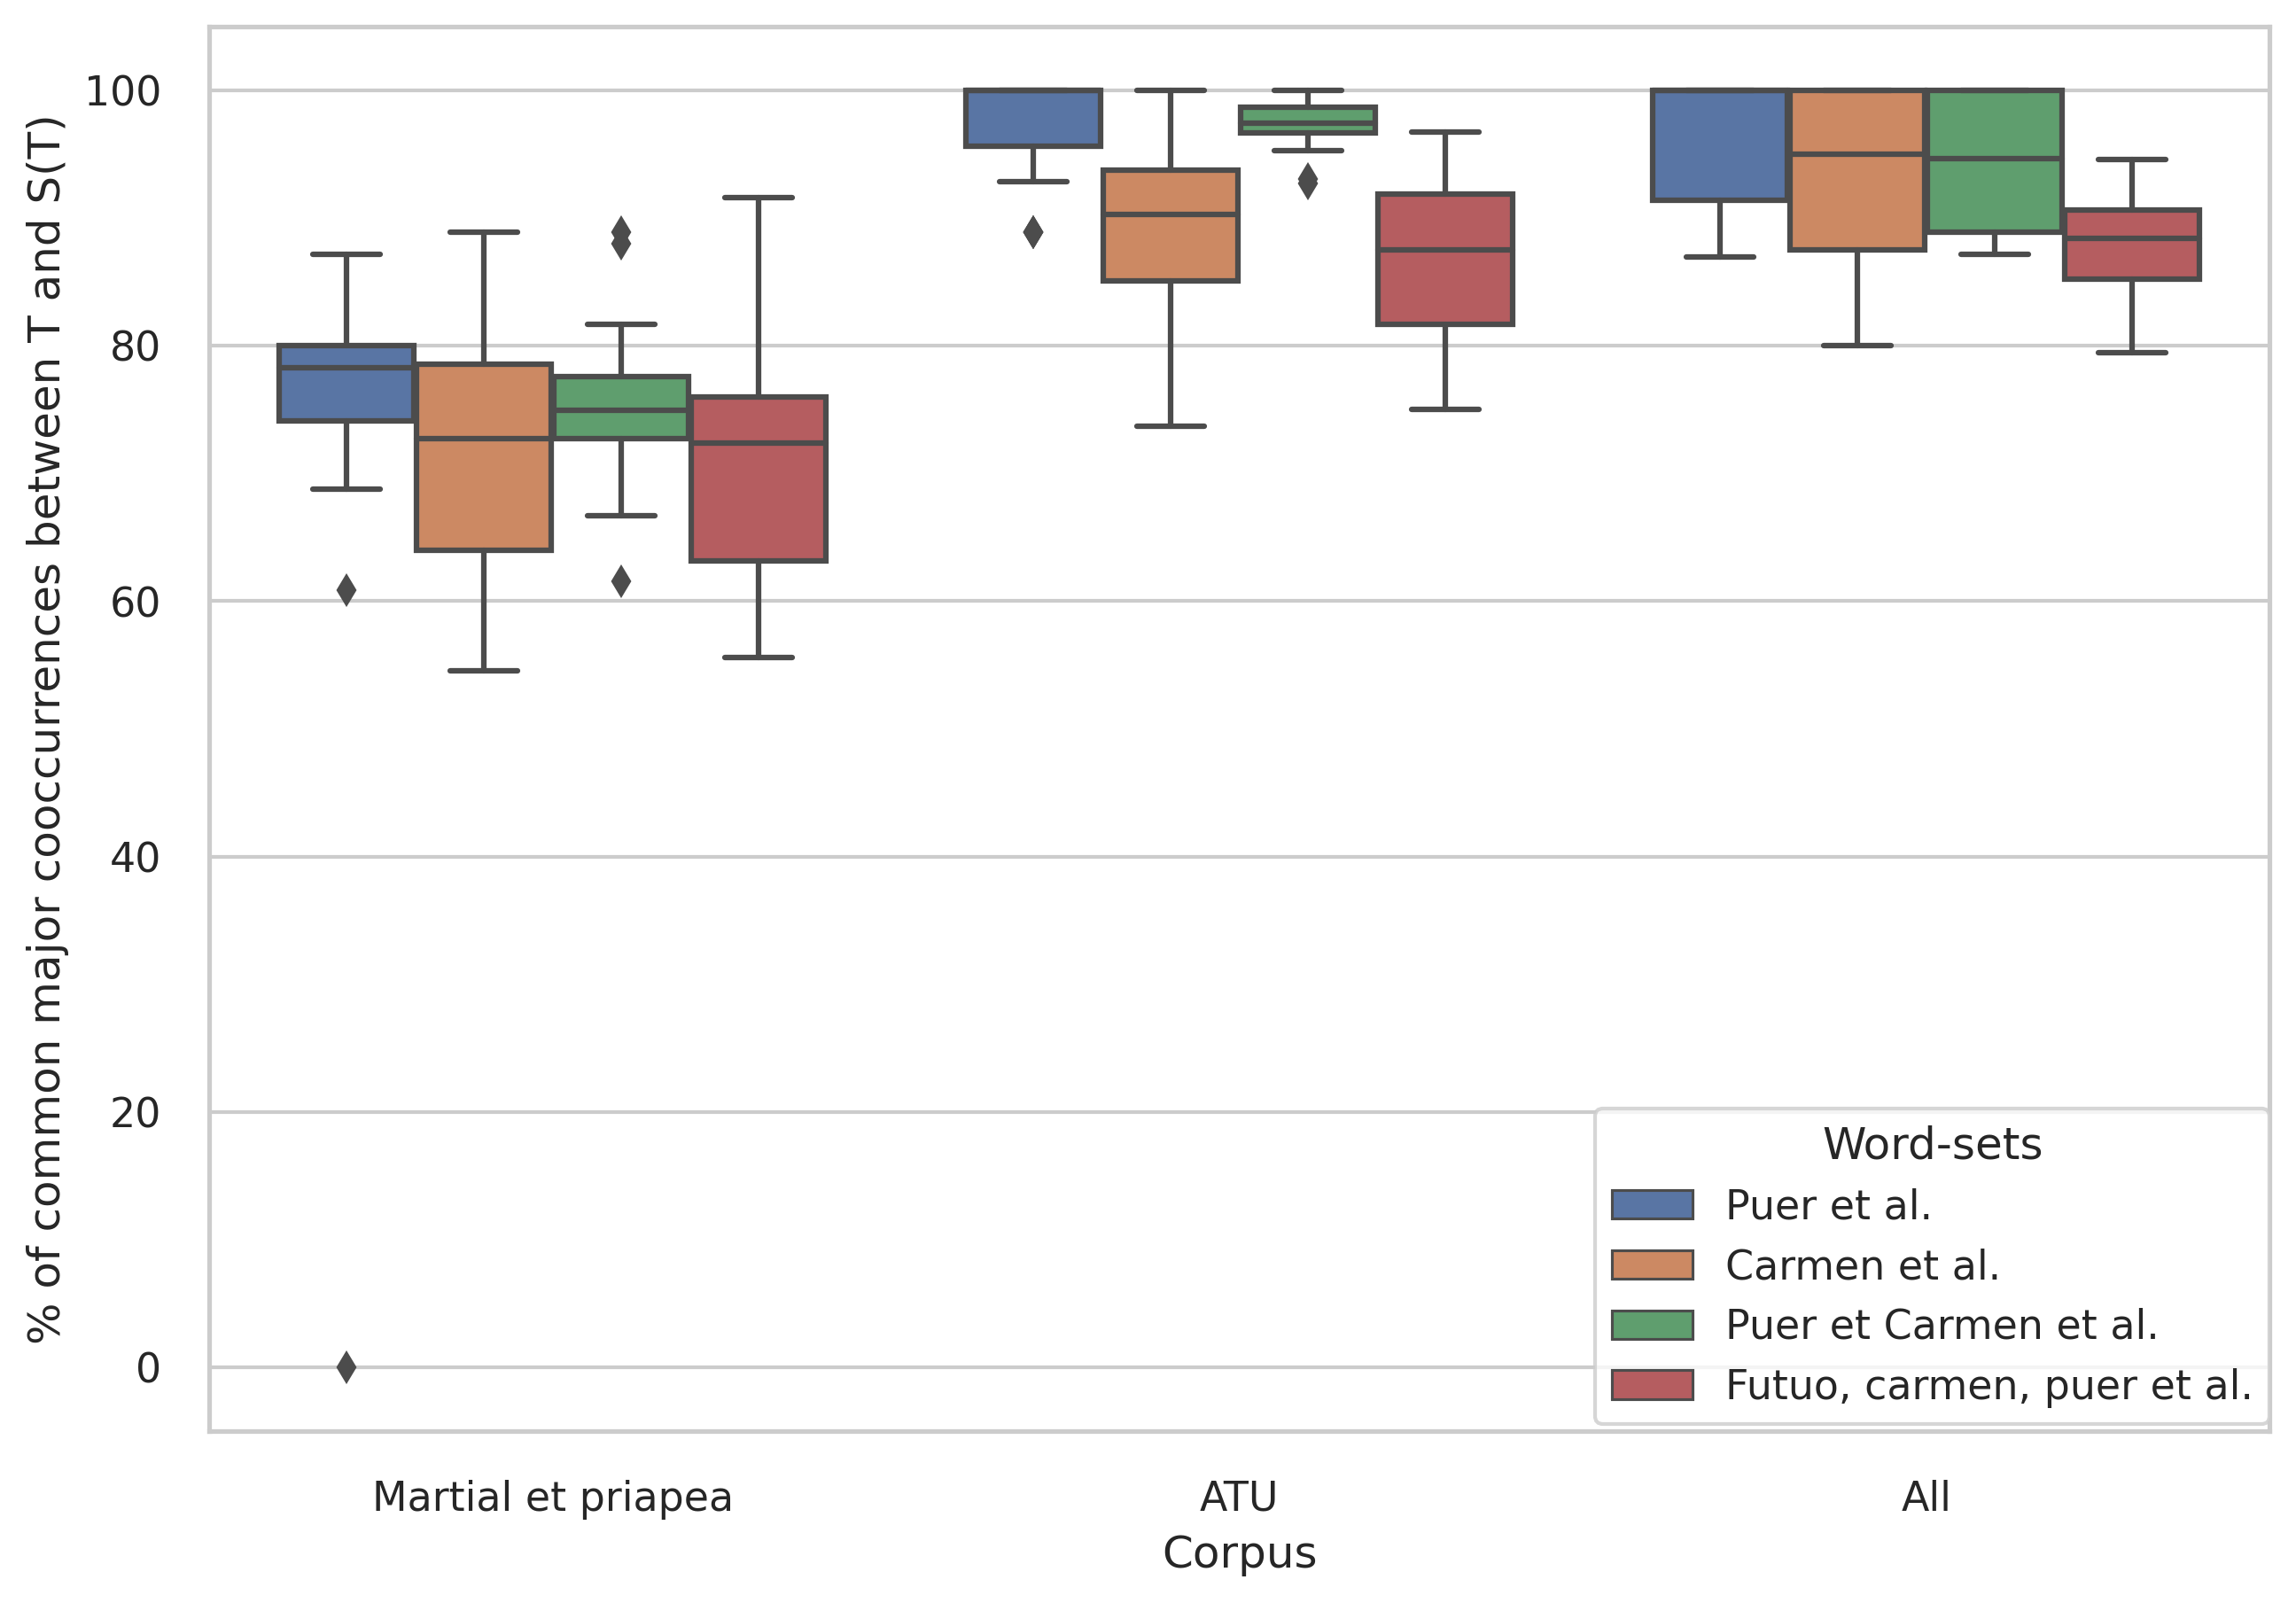
\includegraphics[width=1\linewidth]{figures/chap1/part2/classes_percent.png}
        \caption{Dispersion du \textit{taux de similarité} entre $M_{S(T)}$ et $M_{U(T)}$ pour chaque combinaison de corpus et de mots. Pour \textit{Puer et al.} sur \textit{Martial et Priapea}, les principales co-occurrences ont une similarité médiane inférieure à 80\% sur les 16 combinaisons de $W,F$. Les valeurs aberrantes ne sont pas affichées.}
        \label{fig:classes_de_violon}
    \end{minipage}%
    \hfill%
    \begin{minipage}[t]{.43\linewidth}
        \centering
        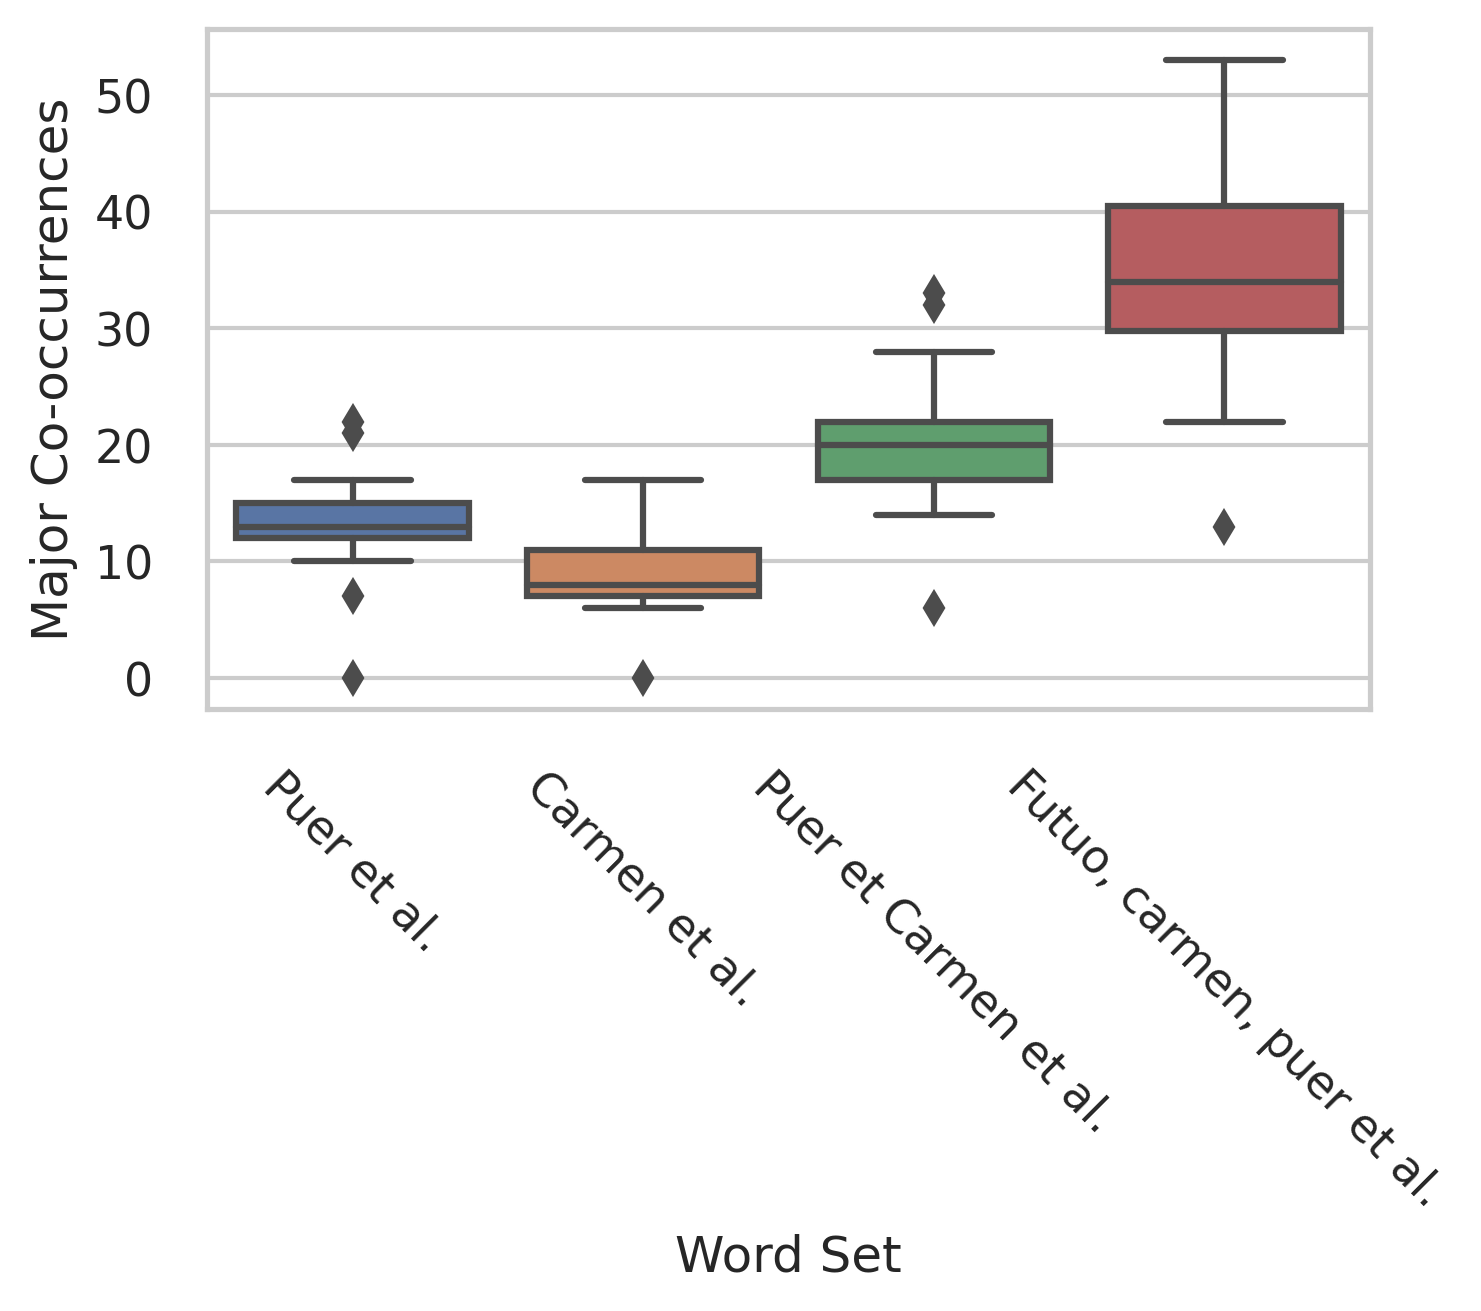
\includegraphics[width=\linewidth]{figures/chap1/part2/major_count.png}
        \caption{Nombre de co-occurrences majeures par ensemble de mots}
        \label{fig:chap1:noise:major_count}
    \end{minipage}
\end{figure}



Cette approche binaire reste limitée et ne donne pas une idée complète de l'impact de l'absence de la segmentation: est-ce un seul mot ou la moitié des composants de $M$ qui diffère entre les deux versions de chaque corpus ? Pour répondre à cette question, nous proposons d'évaluer le \textit{taux de similarité} en fonction des deux ensembles $M$ de co-occurrences majeures, calculés :

\begin{equation*}
    1 - \frac{%
        \left | M_{S(T)} - M_{U(T)} \right | + \left | M_{U(T)} - M_{S(T)} \right |%
    }{%
       \left | M_{S(T)} + M_{U(T)} \right |%
    }
\end{equation*}

À quelques exceptions près sur \textit{Martial \& Priapea} et \textit{Corpus ATU}, le taux de similarité est généralement supérieur à 60\% pour le plus petit corpus, 80\% pour les deux autres \footnote{Voir tableau annexe \ref{tab:anx:noise:capitains:ratio_classes}} alors même que la taille médiane de $M$ se situe entre 8 (\textit{Carmen et al. }) et 34 (\textit{Futuo, carmen, puer et al.)} (\textit{cf.} figure \ref{fig:chap1:noise:major_count}). Quelle que soit la taille du corpus et de l'ensemble de mots, le taux de similarité est globalement élevé: les grands corpus montrent une certaine résistance au bruit, comme nous l'avons vu dans les analyses binaires, et les petits corpus ou groupes de mots à faible fréquence connaissent des variations plus grandes entre $U(T)$ et $S(T)$.

Globalement, les deux métriques montrent cependant un effet incontestable sur la sélection des co-occurrences majeures. Même si la taille du corpus atténue cet effet, comme le montrent les résultats de \textit{All} par rapport aux autres, elle ne garantit pas l'égalité des résultats entre $S(T)$ et $U(T)$, comme le montrent $W=20$ pour \textit{Puer et al.} ou $W=10$ et $W=15$ pour \textit{Carmen et al.}. La manipulation minutieuse des (S)ATU dans des corpus relativement petits ($\leq20M$ tokens) doit être une étape importante pour renforcer toute analyse statistique sémantique, car on ne saurait garantir que les résultats ne soient pas fortement contaminés par de faux co-occurrents.


\paragraph{Sur les caractéristiques}
\label{sub:clustering}

Sur la base de la normalisation de la matrice des co-occurrents des pivots et de $M$, nous voulons identifier si des algorithmes plus avancés étaient aussi sujets à des variations avec cette entrée normalisée. Pour chaque combinaison de $W,F$, on cherche à savoir si les \textit{clusters} $K$ produits par les outils précédemment cités forment une identité de sorte que $K_{S(T)} = K_{U(T)}$ (\textit{cf.} figure \ref{fig:chap1:noise:clusters_rates}). Étant donnés les résultats précédents, impliquant une inégalité courante des $M$, et afin de former avec les pivots un $C$ stable, on s'assure d'abord de filtrer les $M$ de sorte que $C = \text{Pivots} + M_{S(T)} \cap M_{U(T)}$ avant de clusteriser. On ne cherche pas à optimiser $k$, le nombre de \textit{clusters}: il doit simplement respecter la condition $\frac{\left | C \right |}{k} \geq 2$ afin d'avoir au moins deux mots par \textit{cluster} cherché.

\begin{figure*}[ht]
    \centering
    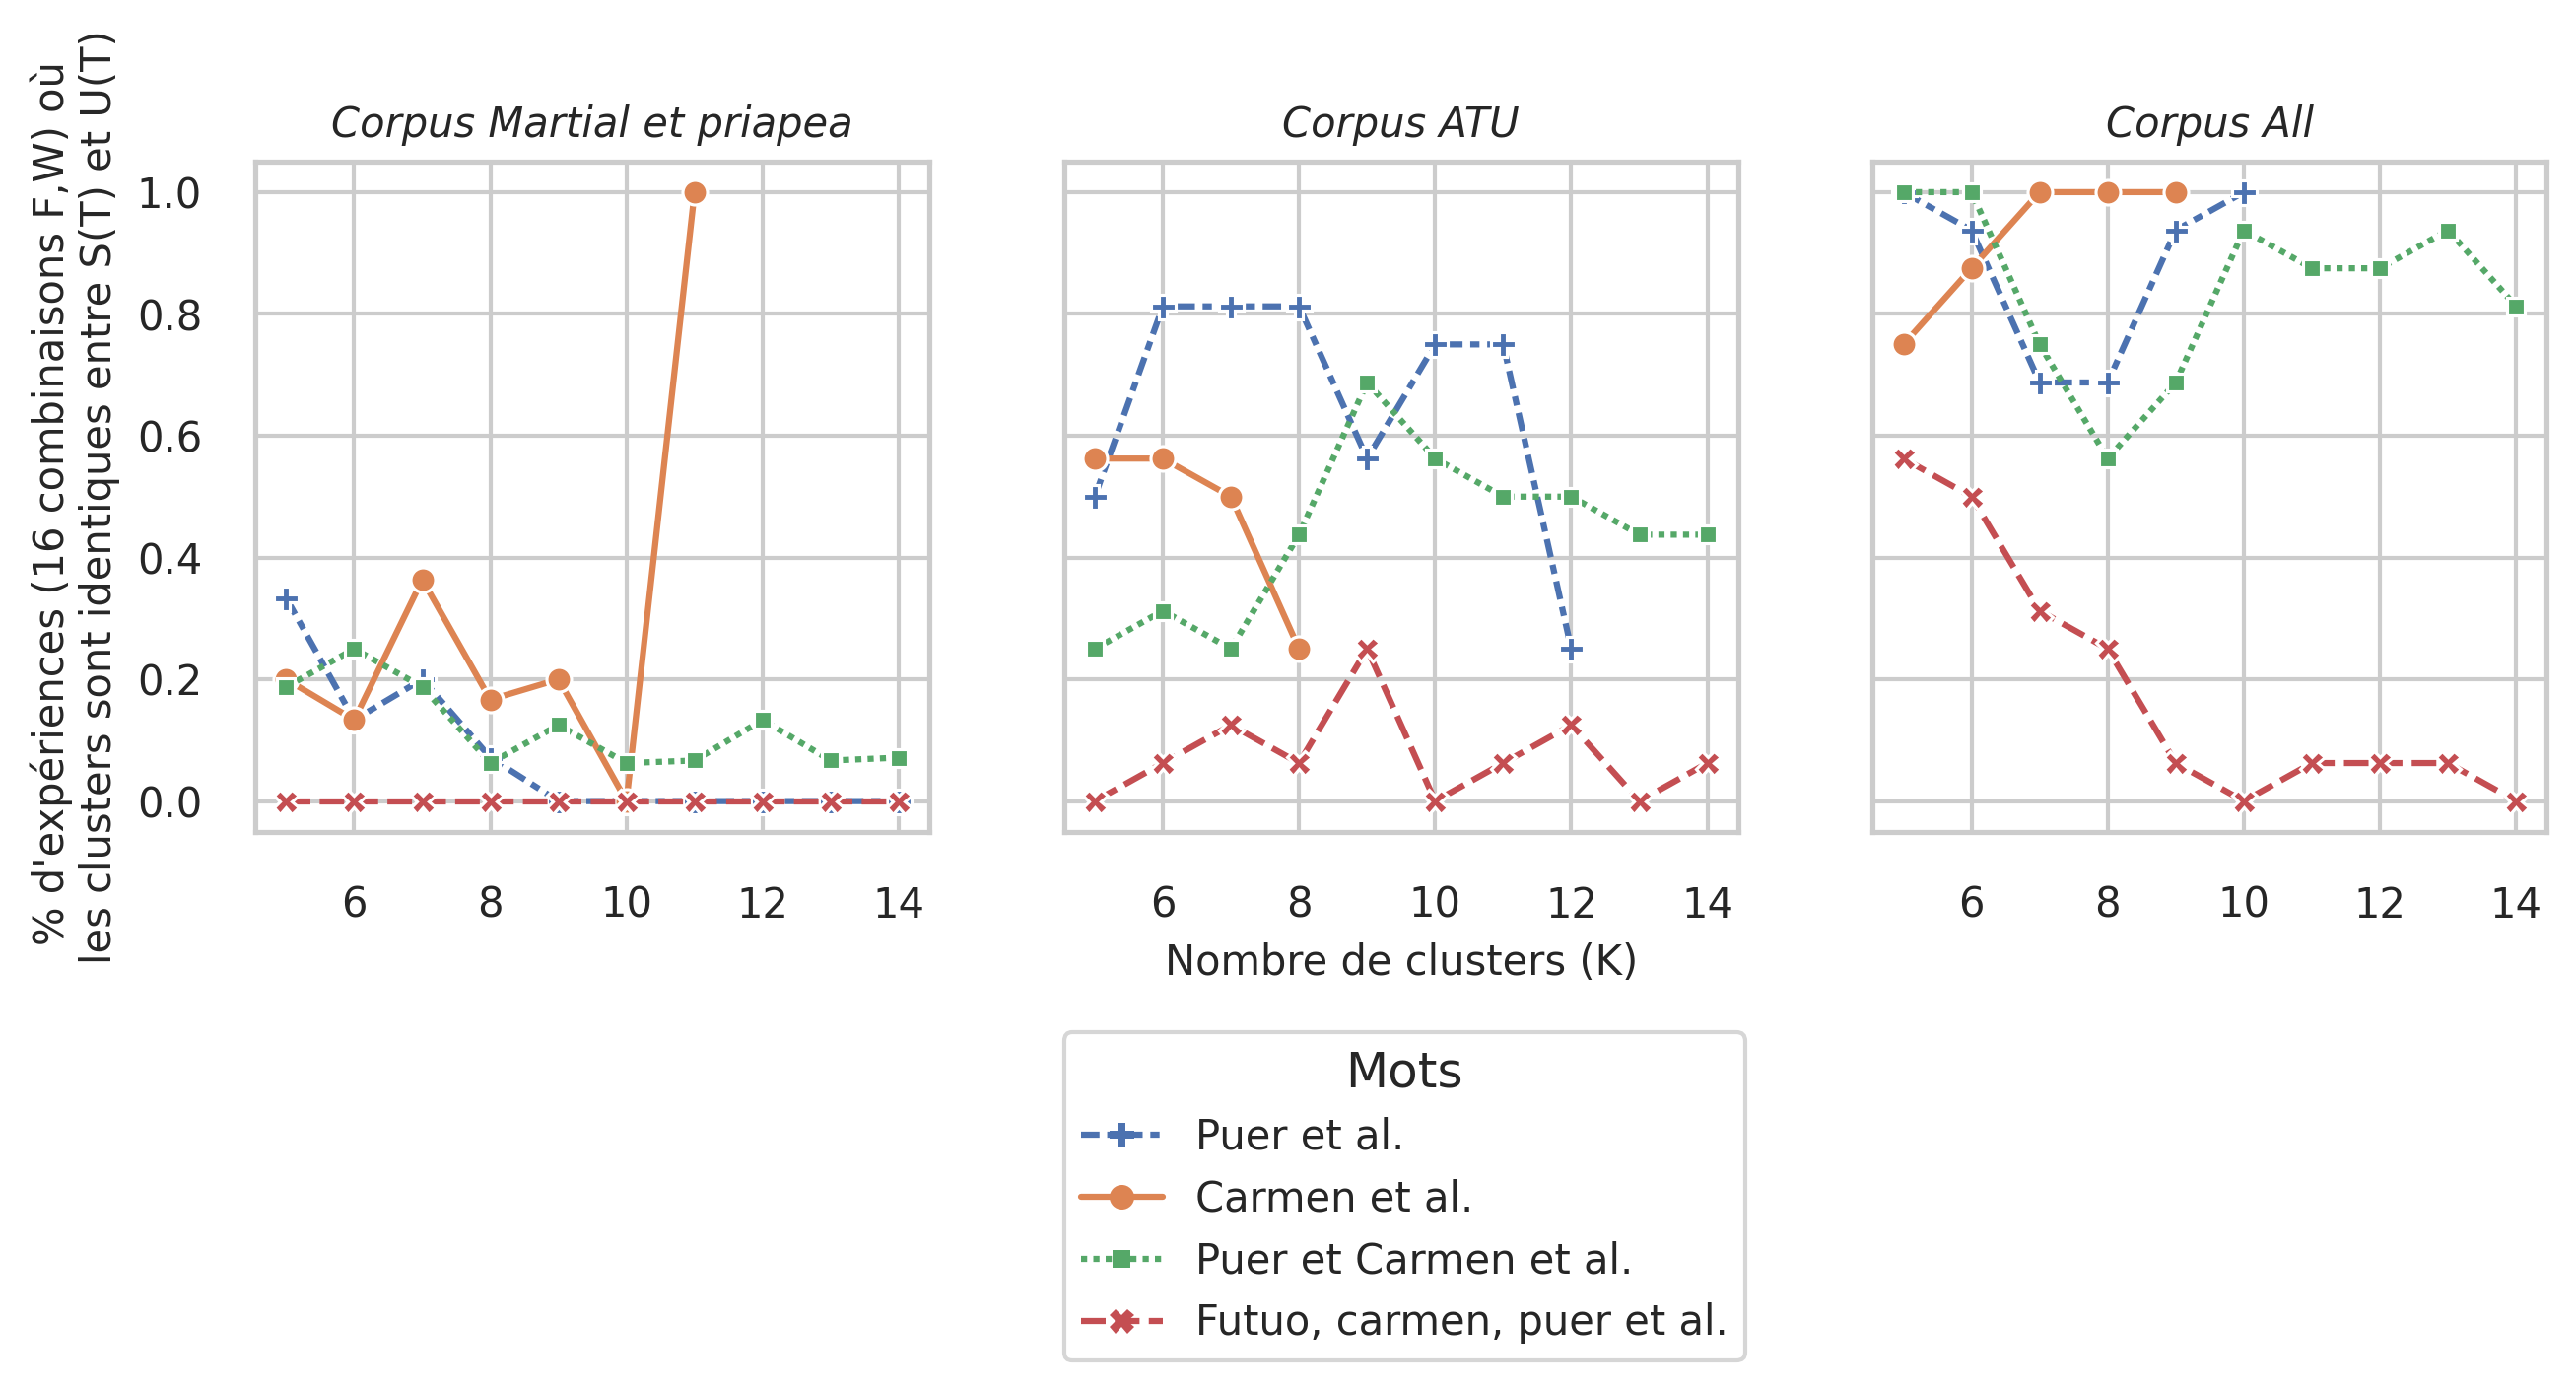
\includegraphics[width=1\linewidth]{figures/chap1/part2/cluster_binary_rates.png}
    \caption{Ratio des expériences où $K_{S(T)} = K_{U(T)}$ étant donné le nombre de \textit{clusters} $k$ et les matrices résultats de chaque expérience variant sur $W,F$ pour chaque corpus et ensemble de mots.}
    \label{fig:chap1:noise:clusters_rates}
\end{figure*}


Dans ce contexte, les caractéristiques ont un impact qui va au-delà de la simple sélection de classes, notamment pour nos deux premiers corpus. Sur \textit{Martial \& Priapea}, quel que soit le groupe de mots étudié, seuls \textit{Carmen et al.} avec $k=11$, parmi l'ensemble des analyses (variant sur $F,W$), produit les mêmes \textit{clusters} pour $S(T)$ et $U(T)$. Aucune des clusterisations sur le corpus \textit{ATU} ne produit le même résultat sur l'ensemble des variations $F,W$ d'une version à l'autre du corpus. En général, moins de 40\% des combinaisons $F,W$ produisent les mêmes clusters pour $C$ sur le plus petit corpus. Comme pour l'analyse des classes, ce chiffre augmente avec la taille du corpus, qui atténue donc en partie l'effet de $S$ sur $T$. Avec 80\% de combinaisons $F,W$ à clusterisations similaires maximums pour \textit{ATU} et 100\% pour \textit{All}. Cependant, cet effet est encore instable et imprévisible: alors que \textit{Puer et al.} atteint 100\% d'expériences ($F,W$) égales dans leur clusterisation entre $S(T)$ et $U(T)$ avec $K=5$ et $K=10$, il tombe à 70\% pour $K=7$ et $K=8$. Cette instabilité s'ajoute au fait que les données ont déjà été \enquote{manipulées} en réduisant les $M$ à un set commun $C$.

\subsubsection{Conclusion de l'expérience}

% Rework CONCLUSION

En 1957, J. R. Firth a utilisé le terme de \textit{company}. Dans notre expérience, il devient contexte pour la lecture humaine et fenêtre pour l'ordinateur. Mais ce que l'auteur entendait est beaucoup plus précis que d'avoir deux mots qui se suivent dans un fichier: il est fort peu probable que, face à deux articles de presse sur une même page, J. R. Firth eut accepté de dire que le dernier mot d'un article est \textit{company} du premier mot de l'article suivant. La réponse devrait être claire pour n'importe quel linguiste ou philologue, et pourtant, les textes et les œuvres composites ont été traités de cette manière par des études en humanités numériques ou en TAL\footnote{\textit{cf.} \textcite{kontges_measuring_2020} par exemple.}. 

Dans cette expérience, nous avons évalué l'impact de la non-prise en compte de la structuration des textes. Bien que le fait de travailler avec des statistiques sur des corpus aussi petits exige par nature de la prudence, nous avons démontré que le fait de traiter les œuvres numérisées comme des unités \textit{de facto} homogènes et indissociables plutôt que comme un patchwork de plus petites unités modifie les résultats de l'analyse distributionnelle avec des corpus comptant jusqu'à une vingtaine de millions de mots. Dans nos expériences, seules quelques combinaisons des différents paramètres communs à ces applications (taille de la fenêtre, seuil de fréquence, taille du cluster) ont donné des résultats cohérents entre un corpus de textes édités ($S(T)$) et une version brute de celui-ci ($U(T)$). Avec des mots fréquents dans tout le corpus, avec une petite fenêtre ($W=5$) et de grands corpus, l'effet du bruit est atténué. En revanche, si ces mots sont plus fréquents dans des œuvres très segmentées comme la compilation de poèmes, la taille du corpus global aura moins d'impact sur la question. 

Ces résultats justifient la nécessité de textes enrichis de métadonnées qui permettent un post-traitement tel que celui permis par CapiTainS et l'environnement TEI XML original. Ils plaident définitivement pour l'utilisation de déclarations de segmentation avec des métadonnées telles que \texttt{CiteStructure}\footcite{cayless_introducing_2021} afin de rendre ces corpus utilisables par des machines. Certes, ils limitent la taille du corpus et ne permettent pas nécessairement d'utiliser toute la richesse des corpus en friche présentés auparavant: mais ils montrent sans appel qu'il n'existe pas de combinaison de paramètres nous assurant une protection complète des contaminations.


\section{Constitution d’un corpus sur l’expression de la sexualité} 

Disposant d'un meta-corpus de près de vingt millions de mots en latin, il est désormais possible de passer à la compilation d'un exemplier. Le \textit{Wiktionnaire} définit un exemplier comme \enquote{une liste d’exemples [Définition 1] ou de citations [Définition 2] à but pédagogique\footcite{noauthor_exemplier_2019}}, pour E. Crespo, il s'agit de la \enquote{feuille
d’exemples sur laquelle un intervenant appuie son exposé oral}\footcite{crespo2011pour}. Sur la base de ces usages, il est important alors de développer une explication de ce qui est entendu par \enquote{exemplier numérique}. Un exemplier numérique partage avec le corpus numérique l'idée d'une collection de textes dans des formats exploitables par la machine, tandis qu'il retient de l'exemplier papier (1) le caractère fragmentaire -- il ne s'agit que de citations, d'extraits --, (2) sa cohérence thématique, (3) sa visée pédagogique. 

Or, pour aborder l'histoire de la sexualité ou son lexique, ce genre de compilations de source semble important pour un renouvellement de la lexicographie ou de l'historiographie, à l'image de ce qui est fait en histoire des femmes avec des projets comme Eurykleia\footcite{noauthor_eurykleia_nodate}. Il faut mettre à disposition un exemplier numérique, requêtable et manipulable, pour mieux cerner la richesse linguistique du latin sur ce thème, tout comme les réalités qu'il recouvre. Les éléments de notre exemplier ne sont que les préliminaires d'un travail de longue haleine, qui viserait à fournir -- dans un objectif pédagogique -- à quiconque les ressources nécessaires pour embrasser le sujet dans sa diversité.

Cette visée pédagogique ne concerne pas que les étudiants ou chercheurs qui souhaiteraient découvrir le lexique spécifique à la sexualité mais aussi les tournures et expressions \textit{ad hoc} ou imagées parcourant la littérature latine. Il s'agit aussi, dans un premier temps, d'enseigner à la machine comment reconnaître un passage, une phrase ou un ensemble syntaxique cohérent, qui présenterait l'isotopie de la sexualité.

En premier lieu, nous présenterons une courte histoire de la lexicographie de la sexualité et de l'historiographie de ce sujet, en appuyant tout particulièrement sur la source presque unique de notre exemplier numérique de la sexualité en latin, à savoir le \textit{Latin Sexual Vocabulary} de J. N. Adams\footcite{adams}. Dans un second temps, nous discuterons de la production de l'exemplier numérique, de ses principes aux méthodes de compilations. Enfin, nous présenterons comme nous l'avions fait pour le méta-corpus ses caractéristiques statistiques.

\subsection{\textit{Latin Sexual Vocabulary} de J. N. Adams: une source unique ?}

\subsubsection{(D)Écrire le lexique latin de la sexualité: une histoire}

\begin{quote}[Avant-Propos]{Michel Dubuisson, \textit{Lasciva Venus: petit guide de l'amour latin}}
    \enquote{``Le latin dans les mots brave l'honnêteté'' disait le bon Boileau. Il est vrai que la littérature latine peut passer, du moins aux yeux de ceux qui l'ont fréquentée en dehors des classes, pour l'une des plus pornographiques qui soit.}
\end{quote}

Dans son ouvrage grand public, \textit{Lasciva Venus: petit guide de l'amour latin}, Michel Dubuisson, professeur de littérature latine, ne ménage pas les attentes de son lecteur dès les premières pages. La littérature latine serait donc \enquote{pornographique}. Mais cette catégorie, moderne, sous-entend aussi de la bouche de l'auteur une graduation. Il y aurait ainsi:
\begin{itemize}
    \item une littérature pornographique et donc \enquote{appelant un chat un chat -- en l'occurrence une chatte (\textit{cunnus})} comme le dit si bien le même auteur quelques lignes plus loin;
    \item une expression plus nuancée que l'on pourrait qualifier d'érotique, parlant d'actes sexuels et de ce qui les entoure sans être aussi cru que le discours pornographique;
    \item une manière d'aborder le sujet de manière neutre, faisant émerger des discours sur les corps, médicalisés ou moralisateurs.
\end{itemize}

L'histoire de ces discours et de leur lexique ont une histoire particulièrement courte: d'un sujet peu abordé au XIX\textsuperscript{e} puis au début du XX\textsuperscript{e}, si ce n'est sous un aspect religieux, son étude a été totalement renouvelée depuis cinquante ans. Nous nous proposons de revenir sur trois jalons de cette histoire, de manière thématho-chronologique: d'abord, à travers les rares publications lexicographiques du XIX\textsuperscript{e}, puis en s'intéressant au renouvellement de l'historiographie de la sexualité, en terminant par celui de la lexicographie aux alentours des années 1970 et 1980.

\paragraph{Le XIX\textsuperscript{e} siècle, premiers glossaires}

Le début du XIX\textsuperscript{e} siècle connaît une formidable double production sur ce sujet et démarre une tradition bi-centenaire des lexiques et exempliers de la sexualité en latin. En 1822, F.~K.~Forberg, conservateur de bibliothèque, publie à Cobourg (Bavière) l'édition de poèmes d'un auteur italien du XV\textsuperscript{e} siècle, Antonio Beccadelli (1394--1471)\footcite{beccadelli_antonii_1824}. Mais la particularité de cette édition est qu'elle est augmentée de tout un commentaire, le \textit{De figuris veneris} (fr. \textit{Des positions de Vénus}), sur les positions et pratiques sexuelles diverses des Romains, appuyé sur des exemples tirés de la littérature latine. Bien plus tard, en 1882, ce traité, rebaptisé \textit{Manuel d'érotologie classique} pour l'occasion\footcite{forberg_manuel_1882}, est traduit par Alcide Bonneau (cette édition sera traduite en anglais en 1884)\footcite{parra1997figuris}. Une autre édition bilingue latin-français est publiée par Henri Daragon sous le titre \textit{De Figuris Veneris (Des formes du baiser)}\footcite{forberg_f_1907} dans la collection des Enfers de la Bibliothèque nationale de France. Le texte en lui-même est constitué, dans son édition originale, de 8 chapitres thématiques (hors introduction): de la \textit{fututio} (pénétration vaginale, 39 pages), de la \textit{paedicatio} (pénétration anale, 23 pages), de l'\textit{irrumatio} (sexe oral lié au pénis, 27 pages), de la \textit{masturbatio} (17 pages), du \textit{cunnilingus} (23 pages), des tribades (homosexuelles femmes, 24 pages), du \textit{coitum cum brutis} (zoophilie, 3 pages), et des \textit{spintria} (positions sexuelles impliquant dans ce contexte plus de deux partenaires, 5 pages). Les thématiques sont donc larges et diverses, comprenant à la fois les questions du sexe des partenaires -- manière anachronique de diviser les sexualités des anciens -- et les questions de ce qui est ou non pénétré. La première traduction française recompose le texte en six chapitres (on note les \enquote{nouveaux} chapitrages des cinquièmes et sixièmes parties \enquote{De la langue} et \enquote{Fantaisies}), là où celle de Daragon est plus fidèle.

%\begin{itemize}
%    \item Page 205-215, \textit{De Figuris Veneris}
%    \item Page 215-254, De Fututione
%    \item Page 254-277, De Paedicando
%    \item Page 277-304, De Irrumando
%    \item Page 304-321, De Masturbando
%    \item Page 322-345, De Cunnilingus
%    \item Page 345-369 , De Tribadibus
%    \item Page 369-372 , De coitu cum brutis.
%    \item Page 373-378 , De Spintriis ( des plans à trois ?: Les spintries sont une sorte d'innovateurs sexuels)
%    \item Page 379 (index des figures) Figurarum Veneris enumeratio,
%\end{itemize}

La deuxième production du XIX\textsuperscript{e} est le \textit{Glossarium eroticum linguae latinae} (\enquote{Glossaire érotique de la langue latine}) de Pierre-Emmanuel Pierrugues\footcite{pierrugues_glossarium_1826}, publié en 1826, soit quelques années à peine après les travaux de Forberg\footnote{Nous en proposons une version encodée en TEI: \textcite{Clerice_Lasciva_Roma_Lexical_2022}}. Contrairement à l'oeuvre allemande, ce glossaire ne propose pas de classement thématique: c'est un lexique spécialisé, qui se lit comme un dictionnaire, et dont les entrées sont généralement fournies de références antiques ou tardo-antiques. La notion de sexualité y est aussi plus large, pour preuve les entrées \textit{Abortio}, \textit{Honor} et \textit{Ornatrices} (femme de chambre, \textit{habilleuse}). Il a la particularité d'avoir \textit{a priori} été copieusement plagié -- au sens moderne --, du moins d'après l'éditeur d'un \textit{Supplementum} en 1911\footcite{pierrugues_supplementum_1911}: il est en effet réimprimé en 1833 à Stuttgart sous le nom de \textit{Thesaurus eroticus linguae latinae} puis \textit{Der erotische Sprachschatz der Roemer} sous le nom de Carl Rambach. 

\begin{figure}
    \begin{minipage}{.45\linewidth}
        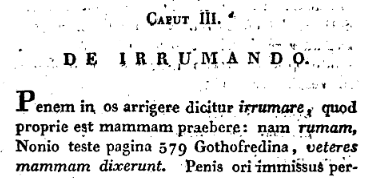
\includegraphics[width=\linewidth]{figures/chap1/part3/277_forberg.png}
        \caption{F.~K.~Forberg, page 277. Le lexique est abordé dans une description plus large des amours latines.}
    \end{minipage}%
    \hfill %
    \begin{minipage}{.45\linewidth}
        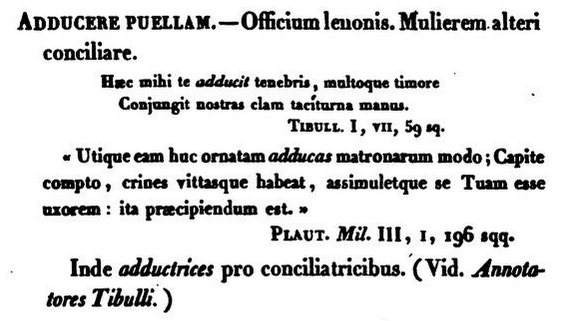
\includegraphics[width=\linewidth]{figures/chap1/part3/13_pierrugues.png}
        \caption{P.-E.~Pierrugues, page 13. Le lexique est écrit comme un dictionnaire unilingue.}
    \end{minipage}%
    \\
    \centering
    \begin{minipage}{.5\linewidth}
        \centering
        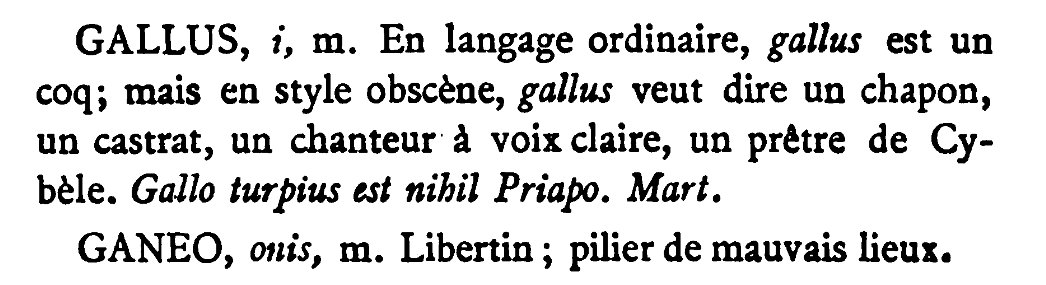
\includegraphics[width=\linewidth]{figures/chap1/part3/62_blondeau.png}
        \caption{N.~Blondeau, page 62. Traduction des termes latins avec explications, quelques citations non traduites.}
    \end{minipage}
    \caption{Exemples d'entrée dans les trois lexiques principaux du XIX\textsuperscript{e}.}
    \label{fig:chap1:exemples_dictionnaires}
\end{figure}

Ce supplément fait figurer des termes de l'ouvrage de Forberg, mais aussi d'un troisième ouvrage publié en 1882: le \textit{Dictionnaire érotique latin-français}\footcite{blondeau_dictionnaire_1885}. Le manuscrit d'origine serait de Nicolas Blondeau, dont on sait par l'éditeur qu'il aurait été avocat, censeur des livres et inspecteur de l'imprimerie à Trévoux en 1695. La preuve de son existence avant son édition provient \textit{du catalogue de la bibliothèque de feu M. Baron}\footcite[Chap. \textit{Belles-Lettres}, p~.2]{noauthor_catalogue_1788} sous l'index 4495, qui le qualifie d'autographe. Mais le texte imprimé en 1882 par Isidore Liseux, dont l'avant-propos nous fournit les éléments nécessaires pour suivre la trace et l'histoire du texte, est en fait un manuscrit à deux mains: le corps du texte est de la fin du XVIII\textsuperscript{e} et de la main de N.~Blondeau, tandis que les notes de bas de page sont issues des annotations d'un second scripteur, ancien possesseur du manuscrit, François Noël. Or, François Noël est bien connu d'Isidore Liseux: ancien enseignant à Louis-le-Grand, \enquote{prêtre défroqué de 1791}\footcite[p.~XVI]{blondeau_dictionnaire_1885}, il a commis l'édition d'un grand nombre de textes autour de la sexualité, de sélections d'épigrammes de Martial aux \textit{Priapées} en passant par quelques florilèges sur le même thème. L'impression du travail de F.~Noël était prévue, d'après les notes de Liseux, mais ne fut jamais mise en route. Cet ouvrage est d'ailleurs merveilleusement relié aux deux précédents, puisqu'il y est inclus un \textit{Essai sur la Langue Érotique} d'Alcide Bonneau, qualifié par son travail précédent \enquote{Traducteur du \textit{Manuel d'Érotologie} de Forberg}.


Les deux ouvrages de la décennie 1820 partagent la même particularité: ils sont entièrement en latin. De fait, il n'est donc pas possible pour l'ensemble des personnes capables de lire d'accéder à la substantifique moelle des travaux présentés, et cette débauche n'est donc disponible qu'aux latinistes, probablement perçus comme plus à même de se contrôler... Ce sont des ouvrages savants, l'un penche vers le manuel, l'autre vers le dictionnaire parfois moralisateur. Cette moralisation est complexe à évaluer, car si d'une part, il donne pour \textit{cunnum linguere} (lécher une chatte) \enquote{\textit{Foeditas Romanis usitatissima}} (\enquote{Horreur des plus répandues chez les Romains}), il appuie cette définition de vers parmi les plus crus chez Martial, issus de l'épigramme VII, 67, où il est question de Philaenis, courtisane et tribade -- on dirait probablement \textit{queer} aujourd'hui -- besognant de jeunes filles et enculant de jeunes garçons. Les deux ouvrages donnent lieu à des équivalents ou des traductions dans la seconde partie du XIX\textsuperscript{e} siècle et au début du XX\textsuperscript{e}. L'histoire du travail de Blondeau et Noël rejoint d'ailleurs habilement celles des travaux de Forberg, en cela que malgré la datation du manuscrit autour des  XVII\textsuperscript{e} et XVIII\textsuperscript{e} siècles, il aura nécessité une forme de réduction de la censure ou de l'auto-censure pour être imprimé à la fin du XIX\textsuperscript{e}.

% Ajouter un truc sur le traditionnel Latin pour traduire le sexe ?

\paragraph{Renouvellement historiographique: construction et déconstruction de mythes ?}

La première moitié du XX\textsuperscript{e} est moins riche en production centrée sur le sujet. J. N. Adams cite dès son introduction deux auteurs, Goldberger\footcite{goldberger_kraftausdrucke_1929, goldberger_kraftausdrucke_1931} et Hopfner\footcite{hopfner_sexualleben_1938}, critiquant abondament le premier\footnote{Cette attitude face aux \enquote{collègues} est d'ailleurs vivement critiquée par Amy Richlin dans son compte-rendu de l'ouvrage d'Adams}. Mais cette traversée du désert touche à sa fin pendant la seconde moitié du siècle, où les renouvellements de l'historiographie et de la lexicographie amènent à de riches productions de savoir.

Il n'est pas question ici de refaire l'historiographie du champ des études classiques, mais d'en montrer quelques points probablement précurseurs de l'état actuel de la recherche autour de la sexualité à Rome. Dans les années 1960, les Annales intègrent définitivement le monde de la recherche sur l'Antiquité, rompant avec l'ancienne tradition. Paul Veyne dit, dans un entretien de 2017, \enquote{[qu']on a cessé de faire des Latins et des Grecs des gens qui représentaient l’humanisme}\footcite{paul_veyne_entretien_2017}, ouvrant ainsi l'étude de l'antiquité à une \enquote{déconstruction} du mythe qu'elle était devenue\footcite{dupont_antiquite_2013}. Cette remise en cause du mythe finit par toucher la question de la sexualité et des corps romains, de l'érotisme: marqueur pour sa génération et point de repère évident, la publication en 1976 par Michel Foucault de \textit{L'Histoire de la sexualité}\footcite{foucault_histoire_1976} devient une référence sur laquelle construire, ou plutôt déconstruire. Cette ouvrage majeur des sciences humaines a posé les bases d'une histoire de la sexualité, ouvrant la porte à de nouveaux questionnements autour des pratiques, de sa fonction dans la société. Mais elle se fonde principalement sur des lectures anachroniques de la société romaine, plaquant les principes d'homosexualité à la Rome antique.

\afterpage{%
\begin{figure}
    \begin{minipage}{0.45\linewidth}%
        \centering
        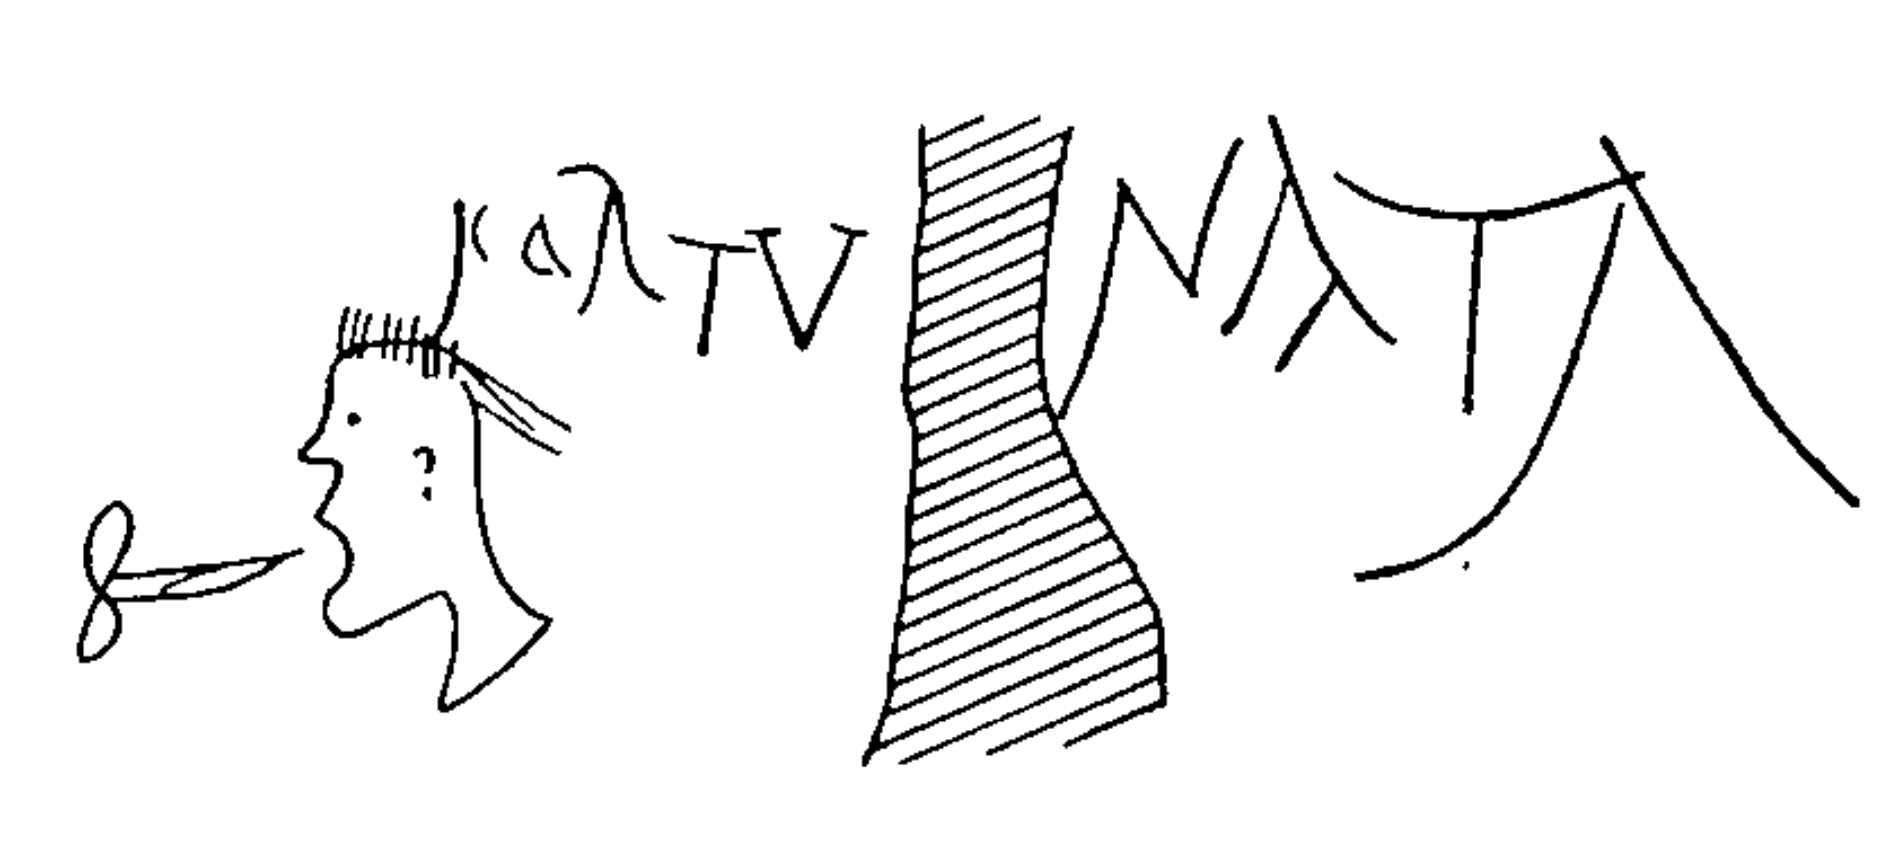
\includegraphics[width=\linewidth]{figures/chap1/part3/graffiti.png}
        \caption{Pompéi, I, 9, 5. Graffiti de \textit{Fortunata} faisant une fellation. CIL, IV, 10005.}
    \end{minipage}%
    \hfill
    \begin{minipage}{0.45\linewidth}%
        \centering
        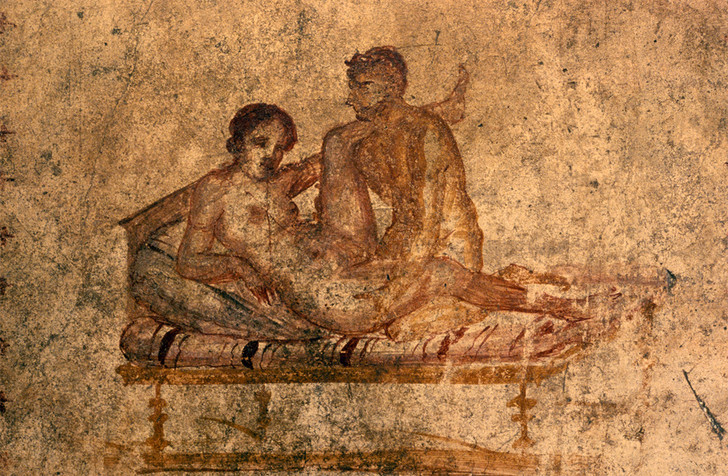
\includegraphics[width=\linewidth]{figures/chap1/part3/vettii.jpg}
        \caption{Peinture érotique d'une pièce attenante à la cuisine de la maison des Vettii (VI, 15, 1). I\textsuperscript{er} siècle. \textcopyright Getty.}
    \end{minipage}%
    \\
    \begin{minipage}{0.45\linewidth}%
        \centering
        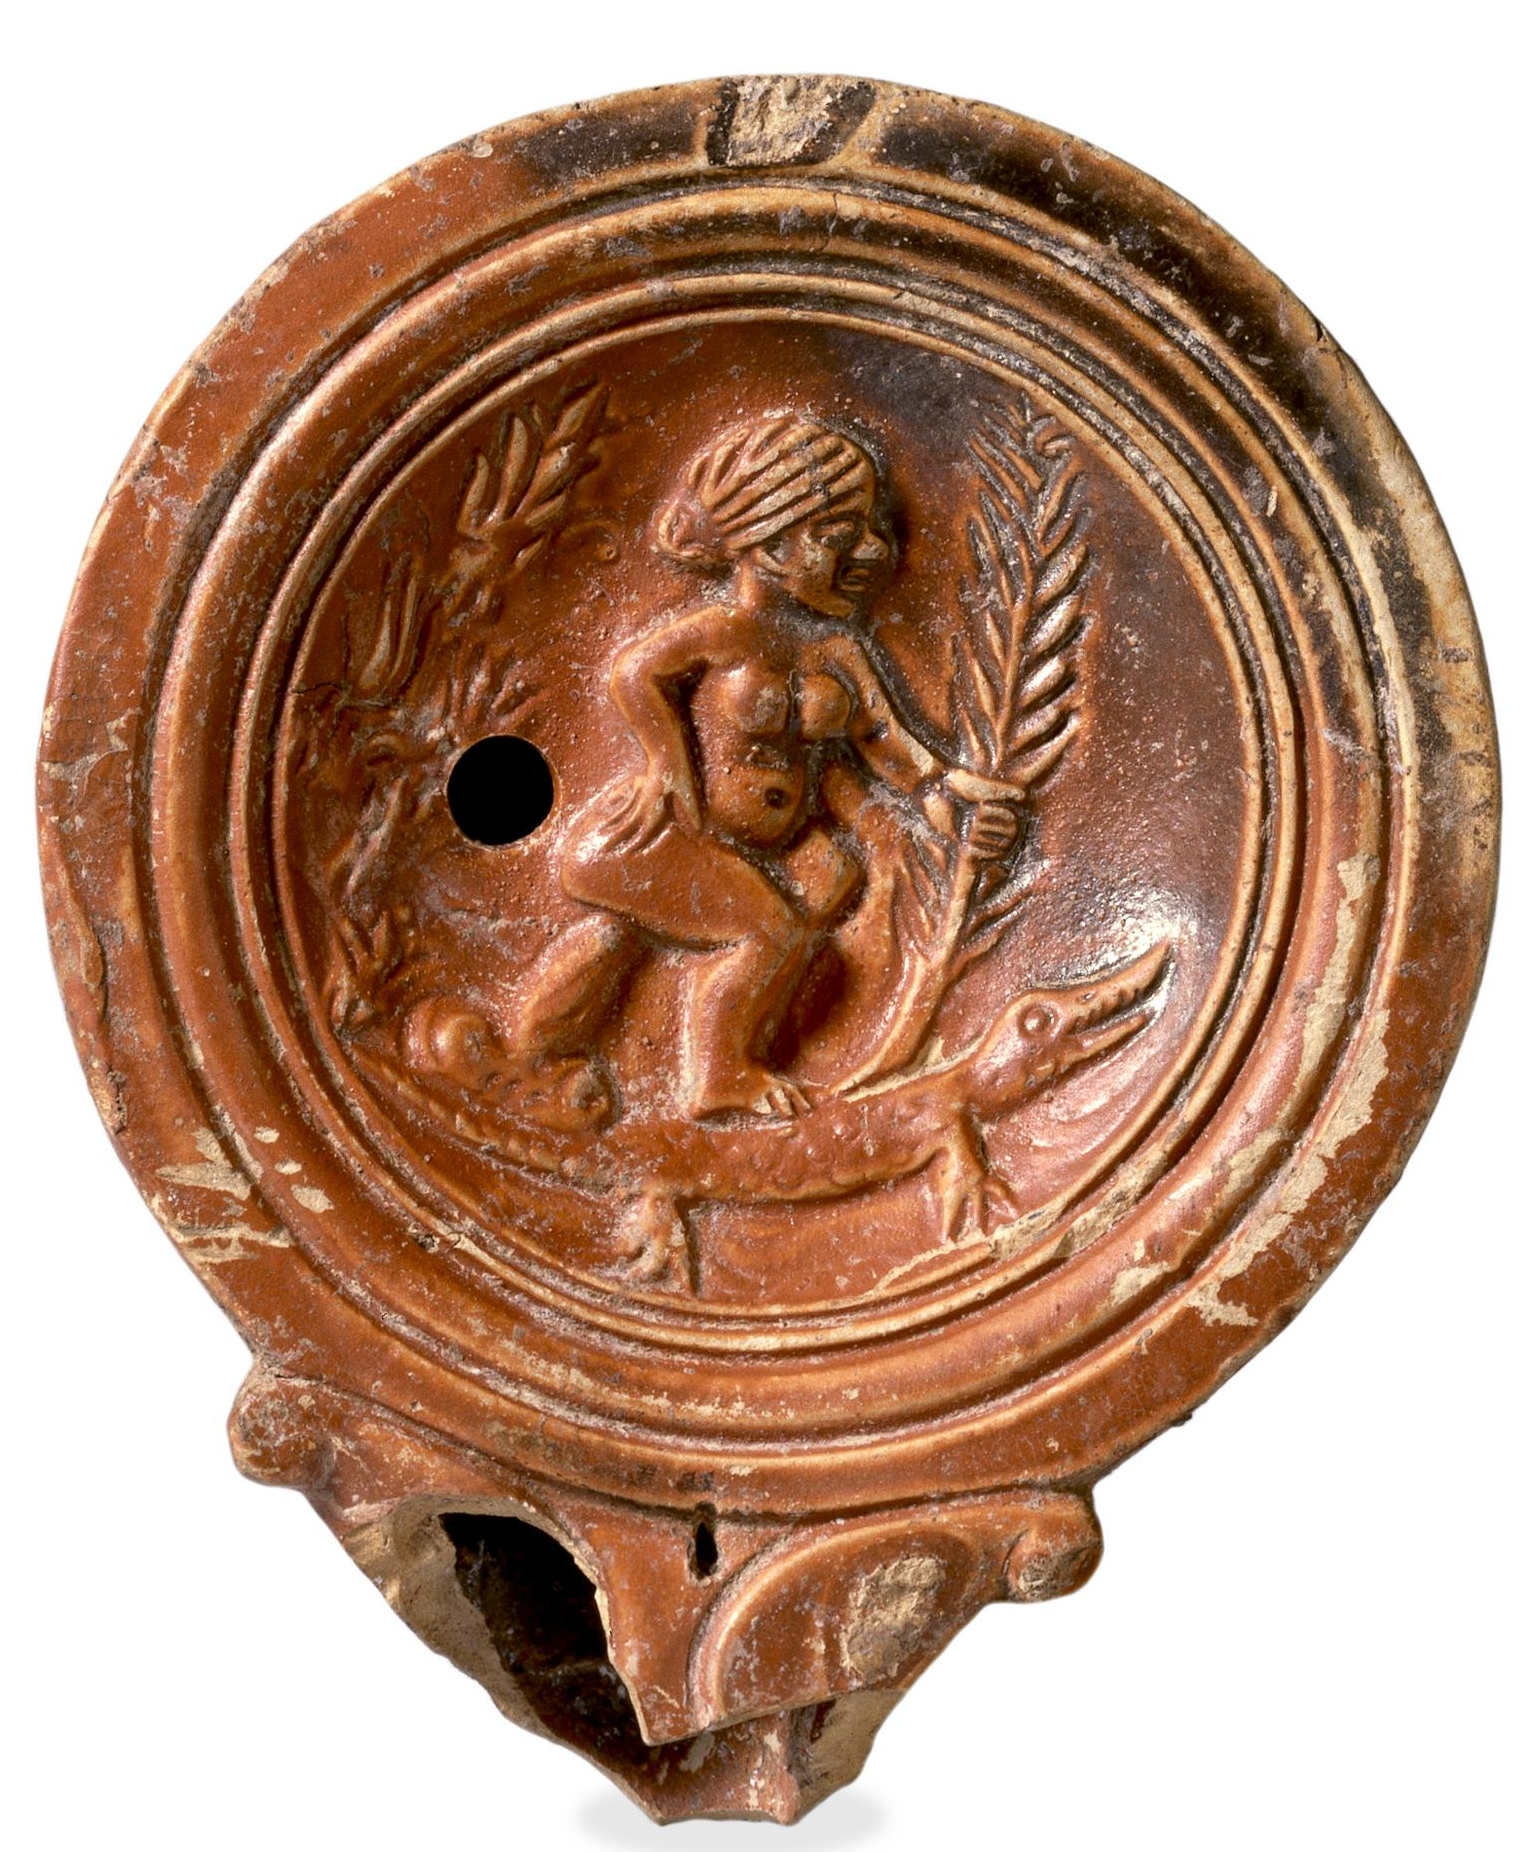
\includegraphics[width=\linewidth]{figures/chap1/part3/36916001.jpg}
        \caption{Lampe en terracota figurant une scène soit d'agalmatophilie avec un Priape, soit de masturbation avec un godemichet. Le personnage est une naine noire égyptienne, caractéristique d'une tendance artistique du I\textsuperscript{er} siècle de notre ère. Entre 50 et 75 d'après Paul G.~P.~Meyboom et M.~J.~Versluys\footcite{meyboom2006meaning}. \textcopyright British Museum, CC-BY-SA-NC.}
    \end{minipage}%
    \hfill
    \begin{minipage}{0.45\linewidth}%
        \centering
        \includegraphics[width=\linewidth]{figures/chap1/part3/Tintinnabulum_Pompeii_MAN_Napoli_Inv27854.jpg}
        \caption{\textit{Tintinnabulum} représentant un Mercure ityphallique. Il manque les clochettes. Museo Archeologico Nazionale di Napoli (inv. 27854).  \textcopyright Marie-Lan Nguyen / Wikimedia Commons / CC-BY 2.5}
    \end{minipage}%
    \caption{Exemples de l'omniprésence des représentations de la sexualité dans la vie romaine.}
    \label{fig:chap1:planche1}
\end{figure}
\clearpage
}

Concernant Rome, on commence à traiter de sujets plutôt personnels, de la vie privée, comme celui de la masturbation\footcite{krenkel_masturbation_1979}. Le travail de Paul Veyne sur l'\textit{Élégie érotique}\footcite{veyne_lelegie_1983} ou l'\textit{Homosexualité à Rome}\footcite{veyne_homosexualite_1982}, se servant à la fois de Michel Foucault et des travaux sur la Grèce de K.~J.~Dover\footcite{dover_greek_1979}, démarre côté français une étude de la sexualité et de l'érotisme romains. Le début des années 1980 reste d'abord un tâtonnement, une phase de questionnement majoritairement conduite à partir de catégories modernes et occidentales. Bien que l'anachronisme permette de poser des questions en histoire\footcite{loraux_eloge_2005}, l'usage de catégories d'analyse contemporaines, comme l'homosexualité, pose un certain nombre de problèmes: la sexualité de même sexe à Rome n'est pas perçue comme opposée à l'hétérosexualité. 

Les années 1990 voient une production de référence avec notamment les travaux d'Amy Richlin\footcite{richlin1992pornography, richlin1993not} ou d'Eva Cantarella\footnote{Publié en 1988 puis traduit en anglais en 1992, \textcite{cantarella_bisexuality_1992, cantarella_secondo_1988}}.%
% Reprendre la relecture ici, page 100
Dans l'ouvrage collectif qu'elle dirige, Amy Richlin entend inscrire son travail dans les \textit{cultural studies}, cherchant donc à donner voix à ce qu'elle perçoit comme les minorités romaines, tout en appliquant les \enquote{théories féministes ou d'autres théories modernes\footcite[p.~XI]{richlin1992pornography}}. Son objectif est aussi de permettre aux \textit{classicists} de reprendre la main sur l'historiographie de la sexualité, et d'aller à l'encontre de ceux \enquote{qui chercheraient la salvation de l'humanité dans un âge d'or passé\footcite[p.~XVIII]{richlin1992pornography}}. Il est alors question de mettre en place un cadre de lecture féministe des textes anciens: se pose la question de la représentation du viol ou en général des violences faites aux femmes. Molly Myerowitz parle ainsi du \enquote{sexisme} ou du \enquote{sadisme} envers les femmes chez Martial, Horace et Juvénal\footcite{myerowitz1992domestication}. Mais ces travaux sont critiqués\footcite{frontisi2004ovide}, pour leur angle et les présomptions effectuées sur la réception des textes par les femmes romaines: une approche émique de la lecture des textes littéraires latins en utilisant des concepts étiques se confronte nécessairement à l'absence de sources et à l'incompatibilité des systèmes, le discours rapporté par les documents transmis étant uniquement celui du groupe dominant\footnote{Tant bien que même si nous avons des textes de femmes, ils seraient probablement aussi issus de cette appréciation de la réalité. \textcite{cuchet_hommes_2011}}.

Les années 2000 puis 2010 voient la naissance -- en France au moins -- d'un renouveau historiographique, héritier en grande partie des pratiques du centre Gernet et des Annales. La question d'un renouvellement des points de vue, quitte à utiliser des approches étiques et donc des anachronismes pour les questionner, permet l'émergence d'une nouvelle histoire de la sexualité, en opposition partielle des approches américaines. Sur la question des sexualités romaines, Florence Dupont et Thierry Éloi préfèrent par exemple les termes homophilies et homoérotismes à celui d'homosexualité\footcite{dupont_antiquite_2013}: il s'agit de différencier alors l'homosexualité identitaire, subie au XIX\textsuperscript{e} puis revendiquée en deuxième partie du XX\textsuperscript{e}, de l'acte sexuel entre deux personnes du même sexe biologique. Il s'agit aussi d'explorer la question des différents objectifs des actes sexuels (récréatifs, reproductifs), de ses interdits, de sa perception et des discours qui les entourent. Géraldine Puccini\footcite{puccini_delbey_vie_2010} cimente ainsi un peu plus les fondements d'une sexualité liée aux statuts (esclave, affranchi, libre, femme mariée, citoyen, etc.) et perçue comme l'on perçoit n'importe quel excès le cas échéant. Le débat historiographique tourne majoritairement -- pour la sexualité masculine -- autour de la thèse de P.~Veyne d'une \enquote{bisexualité active qui suppose la valorisation d'une sexualité virile et conquérante}\footcite[p.~20]{puccini_delbey_vie_2010}, et chacun se situe donc en fonction de cette dernière. Enfin, la sexualité féminine est étudiée\footcite{girod_les_2013}, confirmant une dichotomie entre la femme mariée, au rôle reproductif, et la prostituée, au rôle récréatif, avec des variations entre les deux pôles. On traite enfin d'autres sujets que le simple plaisir masculin: le plaisir féminin et le discours qui s'y rapporte, notamment chez Ovide, prennent leur place dans cette historiographie renouvelée.

En parallèle, la sexualité romaine s'affiche à travers des ouvrages grand public en histoire de l'art. Les travaux illustrés de Catherine Johns\footcite{johns2000sex} ou d'Eva Cantarella\footcite{cantarella_pompei_2000} ont par exemple une vocation: montrer et faire comprendre l'omniprésence du sexe dans la vie et la ville romaine (\textit{cf.} planche \ref{fig:chap1:planche1}). Pour l'époque contemporaine, cette représentation constante des \textit{phallus} et des actes est troublante: du \textit{tintinabullum}, sorte de lampe à clochette permettant par exemple de rejeter le mauvais sort, mais aussi d'annoncer l'ouverture des bains, aux peintures érotiques et graffiti sur les murs, le sexe est partout. Une catégorie d'objets est probablement la plus représentative de cette diversité: les lampes à huile en terracotta, faisant figurer aussi facilement gladiateur que toute une variété de scènes de sexe. Ont été recensées sur ces supports les classiques scènes de fellation, pénétrations anales et vaginales. Les acteurs, leur nombre et les positions y varient fortement: femmes, hommes, nains, dieux, animaux\footnote{Sur ce sujet, la collection du \textit{Romisch-Germanisches Museum} est exemplaire.}. Ce renouvellement, encore bien timide dans de nombreux musées\footnote{Pour préserver la jeunesse d'une telle image ?}, permet de lier archéologie et analyse des textes pour renouveler notre compréhension de cet aspect de la Rome antique.

\paragraph{Le renouvellement lexicographique}

De ce changement d'attitude vers Rome nait un renouveau du travail lexicographique. Jusqu'aux débuts des années 1970, le travail se concentre plutôt sur le parler populaire\footcite{otto_sprichworter_1890} ou la vulgarité latine\footcite{opelt1970schimpfworter} ou encore le style figuré\footcite{opelt1966euphemismus}. Puis, cette décennie voit émerger un un travail directement centré sur la sexualité et son lexique: en 1973, à travers la thèse d'Enrico Montero Cartelle\footcite{montero_cartelle_aspectos_1973} qui nous est connue par M.~Dubuisson, puis en 1978 à travers celle d'Amy Richlin\footcite{richlin_sexual_1978} \textit{Sexual Terms and Themes in Roman Satire and Related Genres}. Les deux auteurs font d'ailleurs de ce domaine une spécialité: E.~Montero~Cartelle continue à publier sur la question sexuelle ou à éditer des textes sur le domaine, principalement du bas Moyen-Âge (\textit{De Coitu} par exemple); Amy Richlin est particulièrement connu pour son travail sur l'histoire des femmes et de la sexualité, comme il a été vu plus haut. 

\begin{figure}
    \centering
    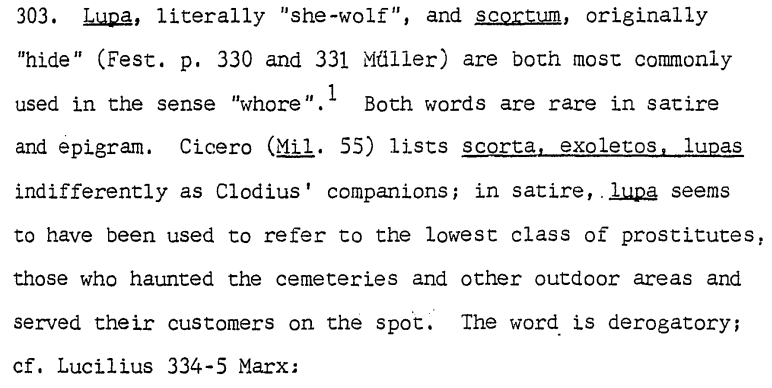
\includegraphics[width=.7\linewidth]{figures/chap1/part3/303_AmyRichlin.png}
    \caption{Exemple d'entrée (reproduite partiellement) de la thèse d'Amy Richlin}
    \label{fig:chap1:entry_richlin}
\end{figure}

Le travail d'Amy Richlin se passe de références aux travaux lexicographiques mentionnés plus tôt, mais établit, en trois chapitres, un état des lieux conséquent. Son premier chapitre et son second permettent d'établir un \enquote{cadre théorique} sur les questions des obscénités en latin et de réparti les sources sur la sexualités en deux sous-catégories, celle de l'\textit{erotica} et celle de l'invective. Contrairement à l'ouvrage qu'elle dirige en 1992, aucune mention n'y est faite des \textit{cultural studies} ou même de féminisme\footnote{Même le terme \textit{reception} n'y est jamais présent.}. Son chapitre trois est un \enquote{catalogue}, plutôt exhaustif dans ses références et dans son traitement de la langue, parfois extrêmement concis et plus proche du dictionnaire. Elle s'inscrit clairement dans la voie tracée par J.~Henderson, lexicographe helléniste, et son \textit{The Maculate Muse} publié en 1976 en lui reprenant ses subdivisions lexicales: \enquote{relation hétérosexuelles; physiologie; rôles hétérosexuels; homosexualité; sexe oral; prostitution; scatologie; caresse et masturbation; piéger et préparer des contextes favorables à la relation sexuelle; divers\footcite[\textit{Abstract}, p.~II]{richlin_sexual_1978}}. Ces catégories sont bien celles du XX\textsuperscript{e} siècle, anachroniques au possible, et se concentrent principalement sur le sexe des partenaires.

Amy Richlin laisse un flou quant aux limites de sa recherche, qu'elles soient génériques ou chronologiques. Du point de vue générique, elle mentionne dans le titre \enquote{la satire et les genres liés}. Ces genres sont en fait beaucoup plus larges que la satire: elle inclut volontiers les discours juridiques de Cicéron dans la catégorie \textit{invective}, mais utilise aussi les inscriptions non littéraires. Les genres plus attendus, comme l'élégie, sont bien sûr présents. Les bornes chronologiques sont courtes, mais floues: la période considérée semble se limiter principalement à l'antiquité classique ou du moins aux écrits païens. Cela exclut de fait des auteurs comme Ausone, dont le travail est inspiré fortement de Martial quand il s'agit de parler de sexualité, ou Apullée\footnote{Cité une fois en note de bas de page page 303.}, dont la peinture du désir masculin est assez exceptionnelle dans la littérature latine. Pour autant, l'\textit{Anthologie Latine} et les inscriptions font nécessairement bouger cette ligne temporelle vers l'antiquité tardive. Au final, la limitation générique est celle qui laisse le plus dubitatif: aucun des historiens latins n'est appelé en renfort par l'auteure pour appuyer les explications qu'elle produit, comme si les gens sélectionnés étaient auto-suffisant pour expliquer le lexique de la sexualité

Les entrées suivent la même structure: elles proposent un lemme et sa traduction ou un thème et les mots qui s'y rapportent (\textit{cf.} \enquote{circoncision}) suivis d'une explication sur les usages et des citations permettant de comprendre les usages du thème. Les entrées sont riches. Elle y décrit les connotations. Par exemple, pour \textit{cunnus}\footcite[p.~208]{richlin_sexual_1978}, l'auteure mentionne les usages poétiques, les exceptions à sa violence supposée, la phrase de Cicéron en \textit{Orat.} 154 pour montrer sa vulgarité\footnote{Cicéron indique qu'il faut éviter de dire \textit{cum nos} (avec nous) car cela ressemble trop à \textit{cunnus} dans ce passage.}, dressant ainsi un panorama complet. On retrouve les contextes d'usage, notamment les contextes génériques: pour \textit{lupa} par exemple, \textit{louve}, elle indique la rareté du terme pour parler de prostituées dans les satires et épigrammes, tandis qu'elle cite les usages de Cicéron\footcite[p.~329]{richlin_sexual_1978}.

En 1982, James Noel Adams publie son \textit{Latin Sexual Vocabulary}, qui constitue notre source principale pour notre exemplier et dont nous parlerons plus bas. Tout au plus peut-on noter une supposition ici sur la chronologie des travaux de J.~N.~Adams et d'A.~Richlin. Cette dernière ne publie jamais son travail de thèse, il n'est disponible que sous forme de microfilms du tapuscrit de 1978. Il est possible que les deux travaux se soient retrouvés en conflit sur le moment, et que celui d'A.~Richlin ait perdu la course à la publication commerciale, tout comme il est possible que la jeune docteure ait souhaité rediriger son travail sur une approche nouvelle du thème, moins lexicographique. Il reste la publication qui suit son travail de thèse, \textit{The Garden of Priapus: sexuality and aggression in Roman humor}, publié en 1983\footcite{amy1983garden}, réutilisant en partie ses travaux de recherche sans valoriser l'ensemble de ses recherches ni adopter la même approche du sujet.
% https://hal.archives-ouvertes.fr/hal-01800658v2/document

\begin{figure}
    \centering
    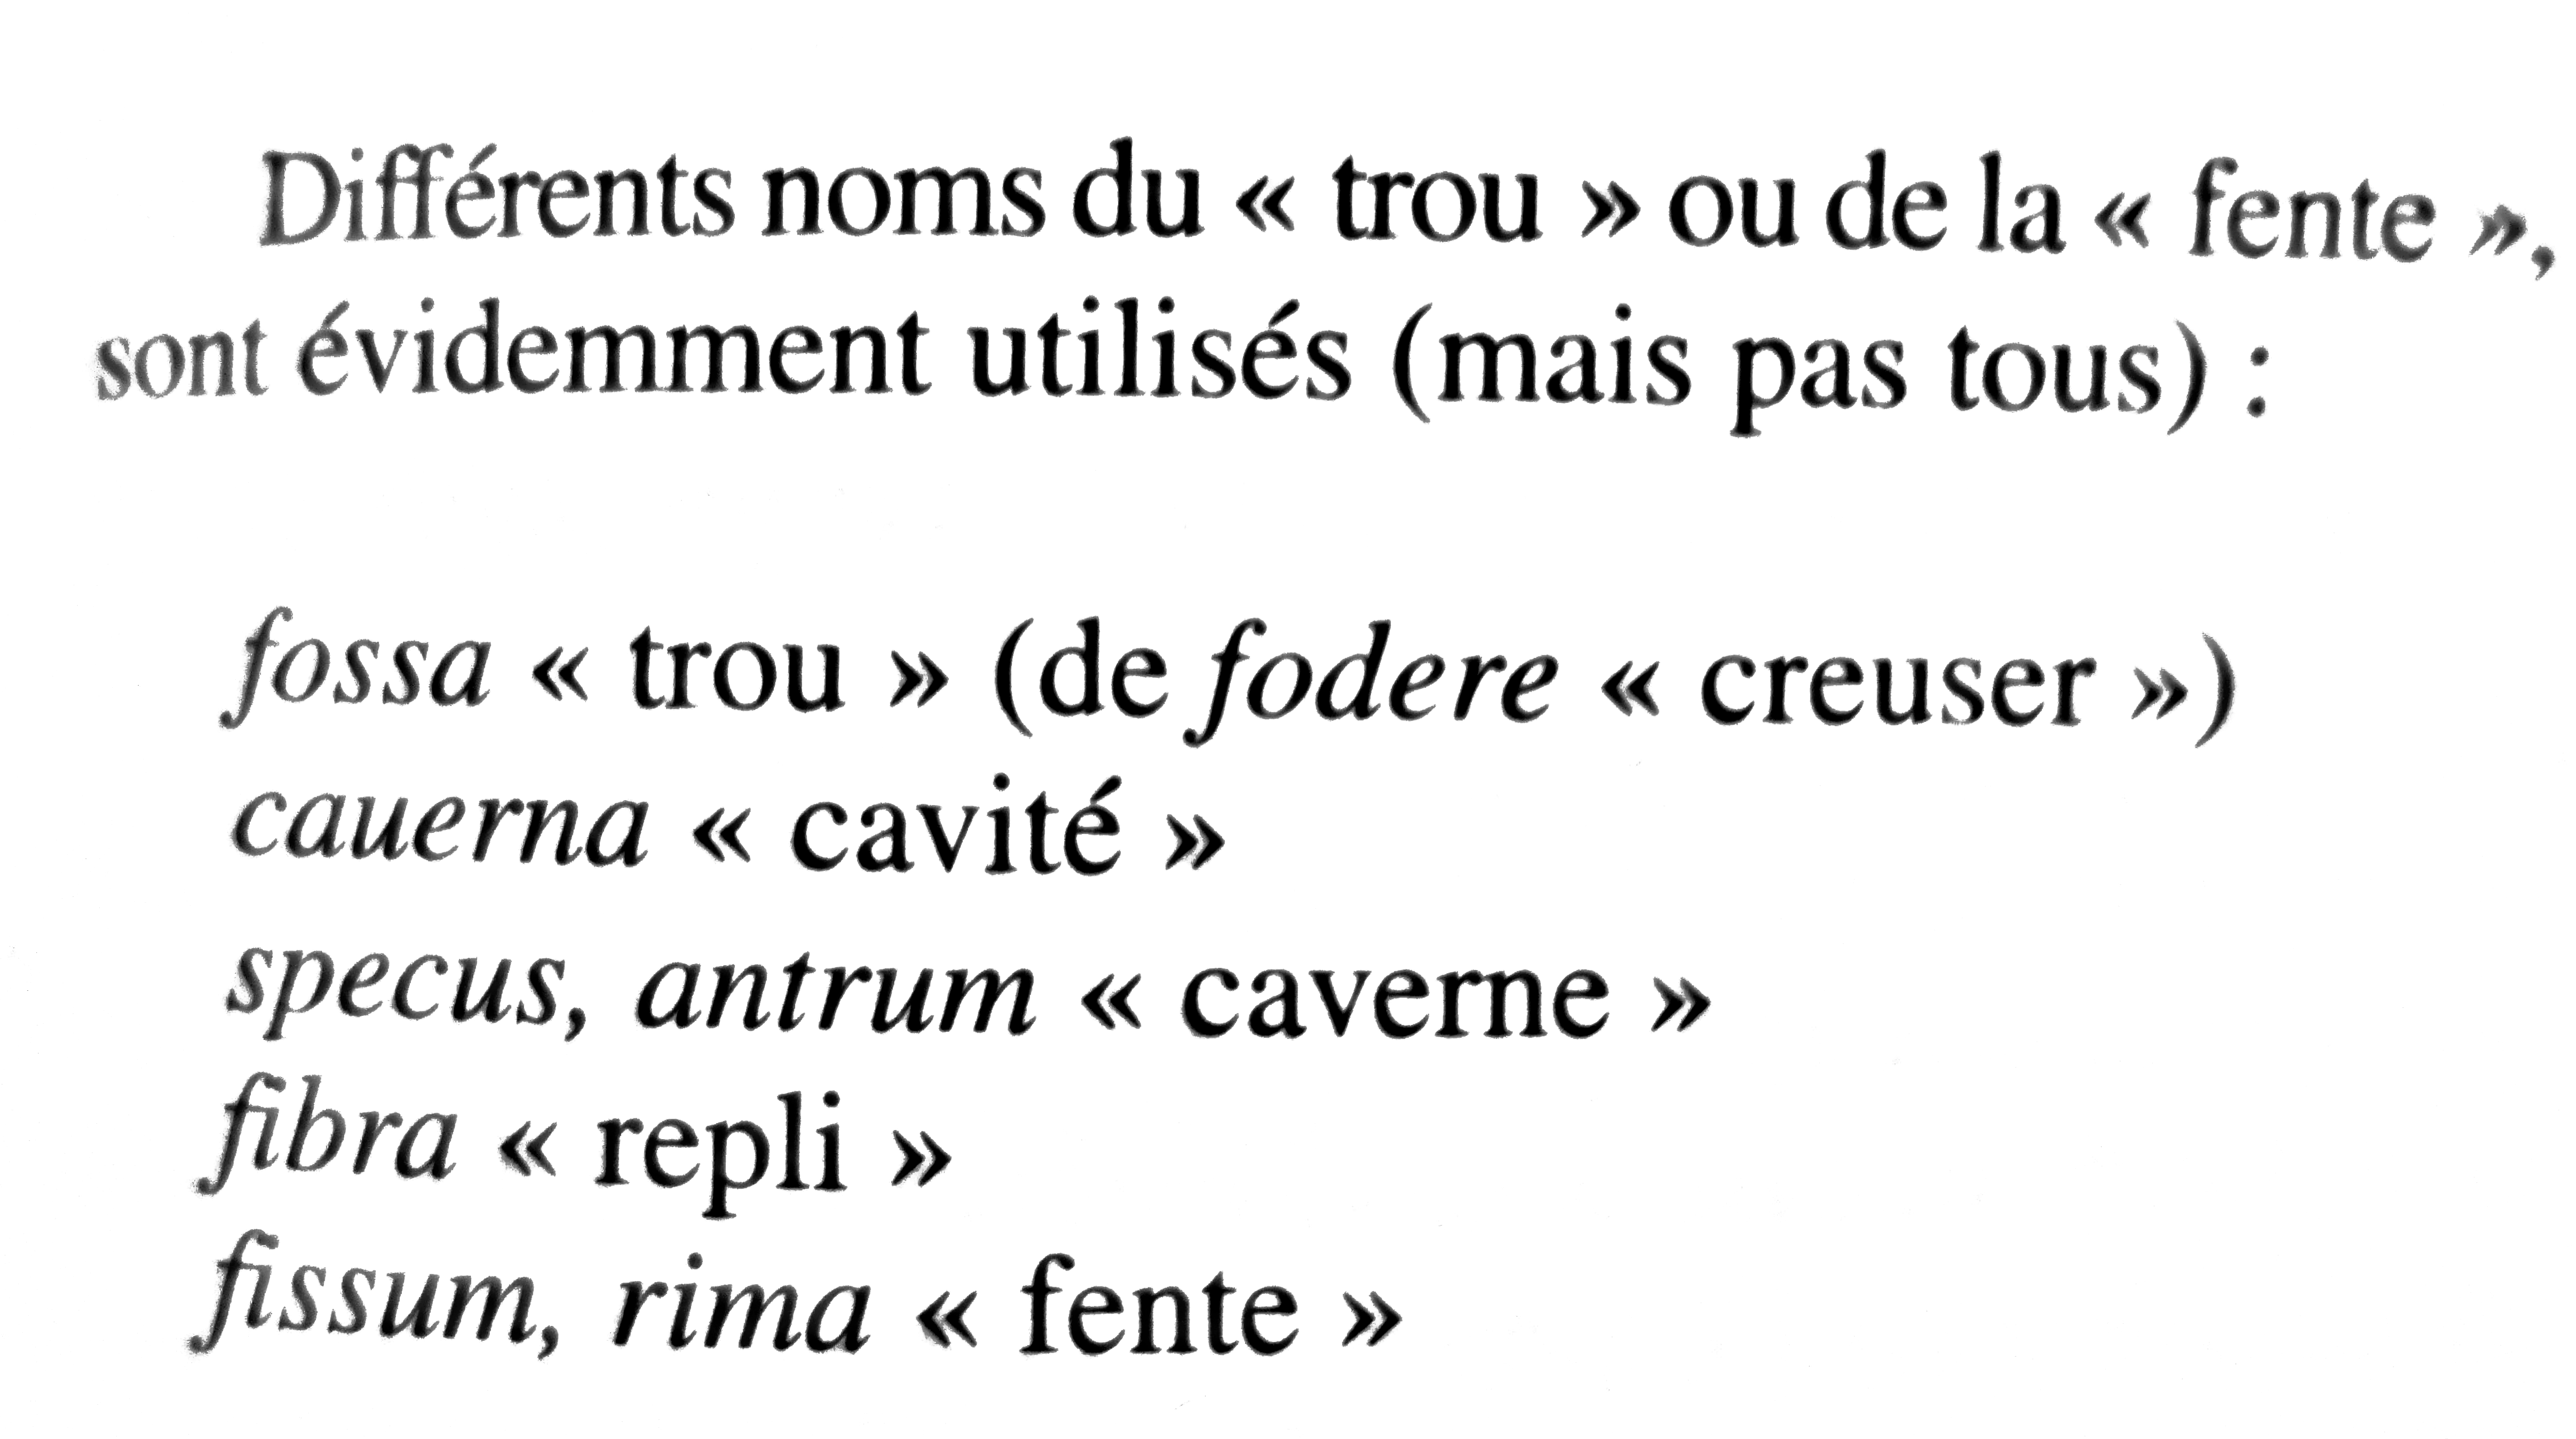
\includegraphics[width=.5\linewidth]{figures/chap1/part3/37_dubuisson.png}
    \caption{Exemple d'\enquote{entrée} de M.~Dubuisson, \textit{Lasciva Venus: petit guide de l’amour latin}}
    \label{fig:cap1:dubuisson}
\end{figure}

Il faut attendre Michel Dubuisson et son ouvrage publié à titre posthume en 2011 pour retrouver une approche lexicographique \enquote{complète} de la sexualité latine. Il y découpe le sujet en quatre parties: \textit{Femina} (corps féminin), \textit{Vir} (corps masculin), \textit{Antecenia} (Préliminaires), \textit{Effectus} (l'acte). Mais le travail de M.~Dubuisson se rapproche plus d'un travail de vulgarisation ou de satisfaction de curiosité intellectuelle que d'une publication scientifique traditionnelle, sans manquer d'érudition cependant. La maison d'édition (La Différence), le ton (\enquote{Ce charmant poème est tout simplement une plainte sur la débandade\footnote{Les qualificatifs charmant et l'usage de \enquote{tout simplement} sortent un peu de la réserve universitaire classique. \textcite[p.~21]{dubuisson_lasciva_2011}}} et l'absence de bibliographie sérieuse (tout au plus quelques références) donnent l'impression que ce livre a d'abord vocation à être lu par des non-spécialistes. Il ne se veut pas exhaustif (\enquote{Je n'avais ni l'envie de faire un pavé rébarbatif, ni la compétence pour faire un \textit{Kamasutra} latin: j'ai dû choisir, c'est-à-dire éliminer\footcite[p.~13]{dubuisson_lasciva_2011}}) et ses choix sont \enquote{criticables} comme il le dit lui-même, peut-être même ancrés dans une vision de la sexualité romaine un peu datée. Mais l'on sent, au fil de la lecture, que c'est un sujet qui amuse, un livre léger, et qu'il s'agissait peut-être pour le linguiste belge de s'échapper un peu de sujets plus \enquote{graves} liés au latin. Il rejoint, nous semble-t-il, le travail de A.~Blondeau au XIX\textsuperscript{e} siècle: la sexualité est un sujet amusant, vendeur, il serait dommage pour l'auteur de ne pas se laisser tenter.


\subsubsection{J. N. Adams, la \textit{Manchester School} et son travail sur la sexualité}

C'est dans ce riche contexte que s'inscrit le travail de J.~N.~Adams, et en particulier sa monographie sur \textit{The Latin Sexual Vocabulary}\footcite{adams}. Mais, si cette effervescence autour des sexualités grecques et latines explose au même moment, il ne faut pas ignorer un contexte beaucoup plus local au travail de l'auteur du \textit{vocabulaire}: la \textit{Manchester School}. Pendant une dizaine d'années en effet, quelques chercheurs des départements de grec et latin à l'université de cette ville se sont spécialisés dans le traitement des obscénités de ces deux sphères linguistiques. Après avoir étudié ce contexte très particulier, nous entrerons dans le détail de l'oeuvre de J.~N.~Adams.

\paragraph{La \textit{Manchester School} de lexicographie}

Le travail de James Noel Adams est absolument indissociable de l'université dans laquelle il a travaillé, à savoir l'université de Manchester. Au début des années 1980, trois de ses chercheurs au moins se concentrent sur la question des obscénités, tant en latin qu'en grec: Henry David Jocelyn (1933--2000), David Bain (1945--2004) et James Noel Adams (1943--2021). Deux de ces chercheurs, Jocelyn et Adams, sont des australiens émigrés, ayant partagé à quelques années d'écart les bancs de l'université de Sydney. Jocelyn a sa commencé sa formation universitaire dans les cours de R.~E.~Smith (1910--1978), professeur d'Histoire Ancienne, y compris à Manchester de 1953 à 1974\footnote{Adams parle d'une profonde influence du second sur le premier}. Il la poursuit au St John's College de Cambridge en 1955\footcite[p.~281--282]{adams_henry_2003}. Il fait son début de carrière à Sydney\footnote{Déroulé de carrière de Jocelyn à Manchester: 1960 \textit{lectureship}; 1964 \textit{senior lectorship}; 1966 \textit{readership}; 1970 \textit{personal chair}.} puis obtient la chaire Hulme de latin en 1973 à Manchester\footcite[p.~286]{adams_henry_2003}. Adams a un parcours similaire: étude pré-doctorales à Sydney puis études doctorales à Oxford avant de prendre un poste à Cambridge jusqu'en 1972 où il rejoint Manchester\footnote{Déroulé de carrière d'Adams à Manchester: 1972 \textit{lecturer}; 1982 \textit{reader}; 1993--1995 \textit{professor}; hiatus dans d'autres universités puis un retour comme membre honoraire à la fin de sa carrière, de 2013 à 2015. \textcite{adams_page_carreer}}. David Bain est au contraire un Britannique au \textit{cursus honorum}, St Andrews (Écosse) puis St John's College (doctorat), avant de devenir \textit{lecturer} pour le grec ancien en 1971 à Manchester\footcite{bain_obituary}. 

Ces trois chercheurs forment donc la \enquote{\textit{Manchester School}}, qui se distingue par le choix de travailler sur les obscénités dans les langues latines et grecques. L'appellation se retrouve à plusieurs endroits, la source de cette dénomination n'est pas claire, F.~R.~D. Goodyear, un ancien camarade de classe de Jocelyn au St John's College\footcite[p.~282]{adams_henry_2003}, semble la faire sienne dans son compte-rendu du livre d'Adams\footcite{goodyear_praefanda_1985}, bien qu'Adams cite un intérêt de la presse pour cette école dès 1983\footcite[p.~289]{adams_henry_2003}. L'auteur du lexique latin de la sexualité fait de Jocelyn le fondateur \textit{a posteriori} de cette école, à travers son article sur λαικαζειν\footcite{jocelyn_greek_1980} et les \enquote{huit autres publications sur la terminologie antique de la sexualité}\footcite[p.~290]{adams_henry_2003}. Il écrit d'ailleurs la préface du travail d'Adams dans sa traduction italienne de 1996\footcite{adams1996vocabolario} où il dresse une bibliographie du groupe. Le travail de Bain nous est connu principalement par cette dernière: il publie neuf articles sur le sujet entre 1978 et 1986, dont \textit{Apotropaic farting}\footcite{bain1986apotropaic}, et puis quelques publications \enquote{tardives} dont son article de 1991, \textit{Six Greek Verbs of Sexual Congress}, où il note justement qu'il s'agit d'une restitution d'un travail commenté dès 1982 dans le séminaire du département de latin organisé par Jocelyn\footcite{bain_six_1991}. 

Le travail de J.~N.~Adams tourne majoritairement autour de la question du latin vulgaire, et par extension seulement il finit par aborder sexualités et corps. Les premiers travaux d'Adams porte en effet en grande partie sur l'édition ou l'étude de phénomènes de langue populaire. Dans \textit{Latin Words for 'Woman' and 'Wife'}\footcite{adams1972latin}, il s'intéresse par exemple à l'usage de \textit{femina} pour désigner une nonne; même dans son travail sur l'ordre des mots en latin, c'est le parler potentiellement populaire chez Plaute (VO plutôt que OV) qui retient son attention\footcite[p.~95]{adams_typological_1976}. Il publie une édition de texte \enquote{vulgaire}, spécifiquement pour le statut de son écriture\footcite{adams_text_1976}: \enquote{[Ce texte] est remarquable par son langage hautement vulgaire. Il a reçu peu d'attention de la part des latinistes, bien qu'il fournisse des éléments importants pour les étudiants du latin vulgaire\footnote{\textit{[This text] is notable for its highly vulgar language. It has received little attention from Latinists, though it yields important evidence for the student of Vulgar Latin.} \textcite[p.~2]{adams1976text}}}. Ce travail donne lieu à plusieurs publications majeures sur le sujet du latin vulgaire, de 1979 avec \textit{The Vulgar Latin of the Letters of Claudius Terentianus (P. Mich. VIII, 467-72)}\footcite{adams_vulgar_1977} à \textit{An anthology of informal Latin}\footcite{adams2016anthology} à 2016, sa dernière publication massive.

Le début des années 1980 sont marquées par le travail spécifiquement lié à la sexualité pour J.~N.~Adams. Trois oeuvres principales (1, 2, 3) sont à lister et plusieurs mineures (4):
\begin{enumerate}
    \item Un article sur le \textit{culus} et les mots qui y sont liés\footcite{adams_culus_1981};
    \item Une monographie, \textit{The Latin Sexual Vocabulary}, publiée en 1982;
    \item Un article sur les Prostitués et les mots pour les désigner en latin, annoncé dans l'oeuvre précédente\footcite{adams_words_1983};
    \item Un article \textit{Martial, 2, 83} commentant le texte dont le titre est issu\footcite{adams_martial_1983}. L'auteur y refait un point sur le verbe \textit{irrumo} (\enquote{enfourcher une bouche}) qui termine le poème. D'autres textes, notamment son travail sur le \textit{Centon Nuptial} d'Ausone\footcite{adams1981ausonius}, complètent aussi son travail de lexicographie par des commentaires longs de quelques sources importantes pour le sujet.
\end{enumerate}
Dans au moins deux de ces travaux (\textit{Martial 2.83} et \textit{The Latin Sexual Vocabulary}), Jocelyn comme Bain sont remerciés\footnote{\enquote{\textit{D. M. Bain and H. D. Jocelyn made some useful comments on a draft of this paper}} dans \textit{Martial 2.83} en note de bas de page}, le premier étant aussi remercié pour l'article sur le \textit{culus}\footcite[p.~264]{adams_culus_1981}. 

\paragraph{\textit{The Latin Sexual Vocabulary}}

La monographie d'Adams est publiée en 1982 chez Duckworth et fait l'objet de réimpression régulière. Elle est accompagnée dès sa sortie d'un \textit{Addenda and Corrigenda} ainsi que d'un chapitre annexe sur les fonctions biologiques hors reproductives (défécation, miction et les flatulences). L'ouvrage comporte 230 pages de rédaction hors préface, annexes, index, bibliographies. Une courte bibliographie principale avec ses abréviations est présentée dès après la préface, et elle est enrichie de références en note de bas de page.

% Le projet d'Adams
Adams présente un projet, en préface comme en introduction, ne cherchant pas à être exhaustif\footnote{\enquote{\textit{I should
not wish to claim that I have been absolutely exhaustive.}}\textcite[Preface, p.~1]{adams}} mais souhaitant \enquote{décrire et classer} la diversité que peuvent présenter les usages latins en matière de sexualités (et d'excrétions). Il s'agit d'un ouvrage rédigé, et non d'un glossaire. Il tourne autour de quatre domaines sémantiques précis, représentés par autant de chapitres, à savoir: le sexe masculin, le sexe féminin, les fesses, les actes sexuels. Ils suivent toujours une progression similaire (Mots de bases, Métaphores, Euphémismes, et, quelques fois, Divers) et s'accompagnent ensuite d'approfondissements spécifiques à chaque domaine, par exemple sur les différentes parties du sexe féminin ou le cas particulier de la masturbation du côté des actes sexuels.

% Couverture thématique: ce qui est présent ?

Chacune des grandes subdivisions de chapitre présente des regroupements: ils sont lexicaux quand il s'agit des termes de bases (\textit{Mentula} est divisé entre \textit{mentula} et \textit{verpa}), principalement stylistiques quand il s'agit d'euphémismes (\textit{pars pro toto}, parties adjacentes, etc.) et sémantiques pour les métaphores. La couverture d'Adams est donc assez large. Par exemple, pour \textit{Mentula}, la section métaphore propose entre autres les domaines sémantiques suivants: objets pointus, armes, objets ménagers, bâtons et choses similaires, objets agricoles, domaine botanique, domaine animale, etc. Adams se permet aussi de produire des sous-sections vides de termes, afin de traiter un domaine où une discussion lui semble nécessaire. Par exemple, pour le sexe masculin, il offre une réflexion sur l'usage de la métaphore du serpent en latin: pour lui, il n'y a rien qui corrobore un possible sème pénien à ces reptiles chez les anciens. Il ne s'agit pas alors de présenter les termes qui sont sexuels, mais ceux qui ne le seraient pas.


% Couverture thématique: Les manques
%   1. manque les adjectifs liés à la sexualité: Lascivus, mollis / mollitia, cinaedus qui n'est pas directement expliqué
%   2. manque les zones autres que sexuelles
%   3. Manque les questions de sex toy ? Aids and Manuals
%       3.a Check ancient sources Sexuality in Greek and Roman societyand literature : a sourcebook,
%   4. Manque des thèmes précis 


Le travail d'Adams démontre un certain nombres de manques. En termes d'avertissement, outre la préface qui annonce la couleur d'un travail massif mais \enquote{non exhaustif}, il annonce aussi page 118 que les termes les plus communs liés à l'acte sexuel seront moins documentés\footnote{\enquote{\textit{Various commonplace verbs and expressions are scarcely illustrated here, especially if the relevant article in the TLL is adequate.}} \textcite[p.~118]{adams}.}. La critique a remarqué cependant bon nombre de mots ignorés, non documentés et uniquement présents à travers des citations\footnote{Chez \textcite{rousselle_j_1987, richlin1984latin}}. Il est possible de répartir une partie de ces manques dans trois catégories: les adjectifs ou appellations spécifiques à la sexualité, les parties du corps sexualisées sans être des organes reproducteurs, et les \enquote{objets auxiliaires} à la sexualité.

Dans la première de ces trois catégories, les adjectifs ou appellations, on retrouve des termes permettent de mieux comprendre les nuances romaines et qui sont par ailleurs traités par A.~Richlin. Par exemple, \textit{lascivus} et les termes de sa famille arrive ainsi en huitième paragraphe\footcite[p.~147]{richlin_sexual_1978} dans son troisième chapitre, très tôt donc, et juste après \textit{futuo} et ses dérivés, \textit{criso}, \textit{salax} (traité rapidement par Adams\footcite[p.~206]{adams}). \textit{Lascivus} peut porter une signification non-sexuelle comme \enquote{joueur, badin} mais aussi pousser ce sens vers la \enquote{disponibilité sexuelle}, donnant ainsi le sens à son dérivé en français \enquote{lascif}. Cet écart d'Adams est d'autant plus intrigant qu'il ne s'empêche pas de traiter des mots proches du sens de \textit{lascivus}: ainsi, son \enquote{\textit{(v) Go, come to}\footcite[p.~175]{adams}} traite entre autres des termes signifiant \enquote{aller au bordel} ou \enquote{venir à quelqu'un en vue d'avoir une relation sexuelle}. D'autres termes suivent le même traitement: \textit{mollis} et sa famille\footnote{Mollis apparaît chez Adams dans des citations uniquement.} ou \textit{cinaedus} permettent par exemple de qualifier les partenaires sexuels. Le léxème \textit{moll-} sert notamment pour souligner la féminité\footcite{williams_meanings_2013} ou les \enquote{abus de plaisir\footcite[p.~320]{dupont_lerotisme_2001}} d'un homme, tandis que \textit{cinaedus} souligne le rôle sexuel du pénétré\footnote{\textcite[p.~142]{puccini_delbey_vie_2010}. \textcite[p.~275]{dupont_lerotisme_2001}}.

La seconde catégorie et la troisième catégorie sont probablement beaucoup moins importante en quantité que la première: les Romains ont tout une richesse de vocabulaire pour parler des partenaires ou des dispositions sexuelles, mais ils parlent moins, dans leur littérature, de certaines partie du corps ou d'objets dans ce contexte. Pour la catégories des autres parties du corps, F.~R.~D. Goodyear, dans son compte-rendu, remarque l'absence des baisers et de la poitrine\footcite{goodyear_praefanda_1985}. Les deux sont traités par Amy Richlin dans sa thèse. Sur le premier, une courte section\footcite[pp.~351--354]{richlin_sexual_1978} sur les baisers (\textit{basium, basio, basiolum, exosculor et osculum}) permet de découvrir un usage des baisers dans un contexte érotique (Pétrone) ou dans le cadre d'une relation à la fellation (en particulier chez Martial). Sur le second, l'auteure les mentionne et en offre une courte analyse\footcite[pp.~229--232]{richlin_sexual_1978}. Il semble que la poitrine, contrairement à la société contemporaine occidentale, ne soit que peu le lieu des fantasmes dans les sources latines. Chez les poètes considérés par la docteure, la mention de la poitrine (\textit{mamma}) se fait toujours dans une invective chez Martial. Au contraire, dans la comédie, elle est vue positivement (usage de diminutifs du type \textit{mammicula} dans Plaute, Pseud. 12961). Le reste des usages sont limités à une description des corps sans une érotisation particulière.

La dernière catégorie est la source d'un traitement plus limité du côté des lexicographes, entre autres car elle est assez rare. Adams, sans en faire une section ni un paragraphe à part entière, relève l'usage de \textit{scorteum fascinum} dans le sens de godemichet chez Pétrone\footcite[p.~63]{adams} mais ne s'étend pas sur le sujet. On retrouve plusieurs autres termes, qui, contextualisés, offrent ce sens dans les quelques travaux qui en parlent\footnote{Sur ce sujet, le plus grand nombre de références est chez \textcite{parker1997teratogenic}}. Chez Ausone 78\footnote{Ausone, Épigramme 76 dans l'édition de B. Combeaud. \textcite[pp.~223-223]{butrica_myths_2005}}, James. N.~Butrica propose un sens parallèle de \textit{lingere membra suae uxoris} (\enquote{lécher le membre de sa femme}) avec le \textit{lambere membra uirorum} (\enquote{lécher le membre des hommes}) du premier vers. Pour l'auteur, il s'agit ici d'un godemichet, et le jeu de l'épigramme tournerait autour d'un mari \textit{fellator} et d'une femme \textit{fututor}. Le même auteur refuse de voir un \enquote{clitoris géant} servant de phallus à Bassa en Martial, 1, 90\footnote{Adams propose la lecture de \textit{venus}$=$penis. \textcite[p.~98]{adams}. \textcite[p.~255]{butrica_myths_2005}}: il propose de voir encore une fois un \textit{sex toy} dans \textit{prodigiosa Venus}. Sans qu'aucun mot ne désigne l'objet en particulier, il appuie sur le sens de \enquote{\textit{pedicare}} quand il s'agit de Philaenis qui \enquote{encule} de jeunes hommes en Martial, 7, 67\footnote{Sur Philaenis, en particulier chez Martial, lire \textcite{boehringer_not_2018}.}. Les godemichets par procuration ne sont pas non plus mentionnés: l'amalgatophilie et l'usage de Priapes en pierre est rejeté en note de bas de page dans le \textit{Latin Sexual Vocabulary}. Il n'y est d'ailleurs fait aucune mention des livres ou manuels liés à la sexualité\footcite[p.185]{puccini_delbey_vie_2010}: le livre d'Élephantis n'est pas mentionné malgré sa présence dans la \textit{Vie de Tibère} chez Suétone\footcite[p.~190]{gladhill_tiberius_2018}.

Au final, il nous semble que la couverture thématique d'Adams se concentre sur la sexualité mettant nécessairement en jeu \textit{mentula}, \textit{cunnus} ou \textit{culus}, et c'est cette sphère qui intéresse l'auteur, comme le montre son annexe sur excrétion et miction.

% Période couverte
%   1. En gros, origine du latin au moyen-âge
%   2. Mais flou entretenu par l'auteur qui ne la définit pas, ce qui se ressent ici aussi.
%       2.a Très mauvaise couverture de la période chrétienne: dépendance du TLL et du canon littéraire ? Ou période chrétienno-tardive moins riche ?
%      2.b TLL et problème du TLL chez Adams

Parmi les autres critiques que l'on peut faire et que l'on a faites au travail d'Adams reste l'importante question des bornes chronologiques de son travail. Or, il n'en expose aucune. Dans le corps du texte, on retrouve quelques mentions du moyen-âge notamment de Babio, auteur du XII\textsuperscript{e} siècle, cité douze fois, ou de \textit{William of Blois} (Guillaume de Champagne), auteur du même siècle que le précédent et cité autant de fois. Cette couverture, nécessairement imparfaite, semble par ailleurs se faire au détriment de l'antiquité tardive, dont la couverture semble être issue majoritairement des mentions trouvées dans le TLL, explicant ainsi une concentration sur quelques auteurs très classiques (Augustin, Arnobe, etc.) au détriment de textes médicaux. La période classique est très bien représentée, en dehors des manques thématiques cités plus haut. Ce travail reste exceptionnel, et il faut le remettre dans le contexte de son époque: il n'y a, en 1982, ni CLCLT ni de PLD, la recherche est intégralement ou presque intégralement manuelle, et on ne peut être qu'impressionné par la masse de données récoltées par le manchesterien.


% Pas de traduction ?
%  1. Adams dit que ça prend trop de place
%  2. Richlin dit que ça fait bizarre
%  3. Jocelyn dit que c'est normal pour un travail de lexicographe

On ne peut pas quitter la description du travail d'Adams sans le replacer à la fois dans sa relation au travail d'A.~Richlin, qui émet un compte-rendu du travail de son collègue australien, et dans son intégration au travail de la \textit{Manchester School}. Dans son papier sur Adams, Amy Richlin\footcite{richlin1984latin} déplore d'abord qu'Adams ne traduise pas, donnant lieu à des situations \enquote{bizarre}: elle cite à cet effet le refus de traduire en page 126 \enquote{Il ne \textit{fellat} pas}, que l'on pourrait rapprocher des pratiques du début du siècle où le latin obscène était laissé sans traduction ou en latin. Cependant, D.~Bain vient à la défense d'Adams\footcite[p.~408]{bain2014praefanda}, plusieurs années plus tard, sur ce même reproche qui lui est fait par une autre auteure\footcite{braund2002personal}:
\begin{quote}[\textit{Prafeanda}]{D.~Bain}
    \enquote{[Elle souligne] l'effet libérateur de l'utilisation d'un langage désinhibé par cette dernière [Richlin]. Cela me semble obscurcir la distinction entre lexicographie et traduction. L'œuvre de Richlin abonde en traductions de passages, en particulier de vers latins, où les obscénités familières anglaises/américaines, si elles sont correctement appliquées (c'est un grand "si"), pourraient bien être utilisées comme une aide pour certains de ses lecteurs. De même, personne ne pourrait critiquer l'utilisation du langage vulgaire anglais dans les traductions proposées par Dover [...] puisqu'il tente de fournir à ses lecteurs des analogies, et que son sujet est plus sociolinguistique que lexicographique. L'étude plus austère d'Adams, en revanche, évite la traduction et vise à présenter un compte rendu lexicographique objectif du ton des mots ainsi que de leur sens. Compte tenu de son intention, il pourrait être considéré comme hasardeux d'avoir préjugé de la discussion en introduisant des termes vulgaires provenant d'une autre langue vernaculaire et d'une autre culture. Je suggère que les lexicographes, lorsqu'ils traitent de cette catégorie de vocabulaire, fassent preuve de prudence.}%
    \footnote{\textit{\enquote{[She stresses] the liberating effect of the use of uninhibited language employed by the latter [Richlin]. This seems to me to obscure the distinction between lexicography and translation. Richlin’s work abounds in translations of passages from, particularly, Latin verse where English/American colloquial obscenities, if correctly applied (this is a big ‘if’), may well be in place as an aid to some of her readers. Likewise, no one could criticize the use of English vulgar language in translations offered by Dover [...] since he is attempting to provide his readers with analogies, and his topic is more a sociolinguistic than a lexicographical one. Adams’s more austere study, on the other hand, eschews translation and is intended to present an objective lexicographical account of the tone of words as well as their meaning. Given his intention, it might be regarded as hazardous to have prejudiced the discussion by introducing low terms from another vernacular and another culture. I would suggest that lexicographers when dealing with this category of vocabulary should practise caution.}}}
\end{quote}
La raison derrière l'absence de traduction tiendrait alors d'une position de lexicographe prise par Adams, tandis que la traduction de Richlin, aussi \enquote{libératrice} soit elle, tiendrait principalement du fait qu'elle traduit les passages\footnote{Ce qui n'est pas tout à fait vrai, puisqu'elle traduit assez souvent les termes hors contexte, quand elle les introduit.}. Et à vrai dire, si l'on regarde les mots même d'Adams, il ne se défend pas ainsi: il cite, tout comme la question de l'exhaustivité, un problème de place s'il se mettait à tout traduire\footnote{\enquote{\textit{The book would be very much longer than it is if I had set out to translate the passages cited, or to discuss at length every crux containing a sexual usage.}}, \textcite[p.~VII]{adams}}. Adams traduit les termes assez souvent, et lorsqu'il ne le fait pas, c'est qu'il le catégorise (\enquote{\textit{Verpa can also be classified as a vox propria for the penis;\footcite[p.~12]{adams}}}).


% Adams, Manchester vs. The World
%   1. Adams et Richlin, un conflit d'approches ?
%   2. Adams et ses collègues: un tradition du bullying universitaire ?
%       Adams sur Jocelyn, page 291 => and then to endure a grilling, particularly from Jocelyn himself, at the end of the paper.
%       Jocelyn was usually sceptical about the attempts of some literary critics to find sexual puns in unlikely places, and this scepticism is nicely exemplified in ‘On some unnecessarily indecent interpretations of Catullus 2 and 3’, in American Journal of Philology , 101 (1980). Liverpool Classical Monthly , as its title suggests, gave contributors the chance to publish their thoughts without the reflection imposed by more conventional forms of publication. Jocelyn, typically, welcomed this opportunity for instant controversy. p. 290

Le deuxième grief qu'Amy Richlin oppose au travail d'Adams est son manque de \enquote{politesse\footnote{\enquote{\textit{A final word on courtesy}, \textcite[p.~494]{richlin1984latin}}}}. Adams est particulièrement violent verbalement avec la littérature scientifique à laquelle il s'oppose, le relevé du comte-rendu est assez exemplaire: il qualifie ainsi le travail d'autres de \enquote{"\textit{totally implausible}" (p. 29, n. 2), "\textit{absurd}" (71, n. 3; 100, n. 1), "\textit{fanciful}" (155, n. 1), "\textit{far-fetched}" (171), "\textit{an absurdity}" (172), "\textit{quite unacceptable, . . ludicrous}" (210), "\textit{bizarre}" (211), or "\textit{so inaccurate that I have chosen not to refer to it}" (1, n. 2)\footcite[p.~494]{richlin_sexual_1978}}. Si l'on rajoute par dessus cela l'opposition des méthodes d'Amy Richlin et de James N.~Adams et le rejet du second du travail de Dover sur lequel la première fonde la structuration de son lexique, il est clair que le travail des deux est en conflit ouvert, comme le montre par ailleurs la reprise du sujet par Bain vue plus haut. Sur ce point, il est amusant de lire la personnalité qu'Adams peint quand il parle de son troisième collègue de la \textit{Manchester School}: Jocelyn aurait été connu pour sa capacité à \enquote{cuisiner} et à faire endurer aux participants de son séminaire ce genre de pratique\footcite[p.291]{adams_henry_2003}; il était de nature à chercher la \enquote{controverse à tout prix\footcite[p.290]{adams_henry_2003}}. Le vocabulaire d'Adams est probablement en partie issue de pratiques Manchesterienne ou d'une influence de Jocelyn sur sa propre manière d'écrire en 1984: après tout, Jocelyn a publié en 1980 un \enquote{\textit{On some unnecessarily indecent interpretations of Catullus 2 and 3}}.

Au final, le travail d'Adams, bien que non exhaustif dans les catégories qu'il couvre et incomplet en terme de thématiques abordées, est probablement devenue la référence sur le sujet du vocabulaire de la sexualité. Il couvre plus de huit cent termes dans quatre grands domaines, en contexte, et documente abondamment les éléments qui l'intéressent. Accompagné de ses articles sur le \textit{culus}, la prostitution, Martial et le \textit{Centon nuptial}, et en général de sa production de 1980 à 1985, il permet d'avoir accès à un panorama conséquent de la richesse lexicale et stylistique du latin pour parler de sexe.

% Compléter Adams ?
%   1. Le travail d'Adams pour compléter Adams
%   2. Les autres travaux

% 

\subsection{Un \enquote{exemplier numérique}}

Pour notre version de l'exemplier, nous utilisons uniquement \textit{The Latin Sexual Vocabulary} d'\textit{Adams}, et les sources secondaires auxquelles il renvoie quand il ne souhaite pas donner, par manque de place, l'ensemble des références. L'exemplier numérique produit a donc deux buts: d'une part, il doit permettre une lecture humaine, d'autre part, il doit être facilement exploitable par la machine. Pour avoir une vue d'ensemble sur cet exemplier, nous discuterons d'abord les principes et la méthode de sa compilation. Nous développerons ensuite une analyse quantitative de l'exemplier numérique ainsi produit et traiterons brièvement de sa valorisation en dehors de l'apprentissage machine.

\subsubsection{Principes généraux}

% Bornes typologiques et chronologiques du corpus
    % Les données épigraphiques: pourquoi non.
        %% Difficulté de lemmatisation
        %% Présence relativement faible
    % Pas les données médiévales
    % Exception: les auteurs fragmentaires

% Format d'un exemplier numérique
    % Pas le premier mais combien publiés en TEI ou SQL ?
    %    Exemple : https://www.pantheonsorbonne.fr/page-perso/e0g411r066s
    %    Helene Castelli, http://theses.fr/2020PA01H075
    %    Eurykleia
    % Sourçable
    % Corrigeable (déjà des idées avec les bibliographies contradictoires ou supplémentaires)
    % Augmentable
    % Pas le premier mais vocation à être à la fois un corpus de recherche ET un corpus d'entraînement. Quel impact ?

Les exempliers numériques ne sont pas nouveaux, particulièrement en histoire ancienne ou en littérature, où la compilation d'extraits pour appuyer une recherche, notamment doctorale, est assez commune\footnote{Par exemple, \textcite{castelli__2020, montreuil_histoire_2016}}. Ces compilations dépassent rarement l'outil d'aide à la compréhension de la thèse et sont assez peu publiées en tant que produits de la recherche. Or, ils pourraient permettre d'offrir une porte d'accès à des chercheurs débutants sur ces questions tout comme ils simplifieraient leur étude pour les spécialistes. Adams, quand il publie son oeuvre, ne la pense pas comme un glossaire comme ses prédécesseurs. On peut probablement voir dans \textit{The Latin Sexual Vocabulary} une forme de base de données, mais c'est avant tout un commentaire scientifique. Passer d'Adams à un exemplier n'est donc pas seulement une collecte, c'est aussi le fruit à la fois d'une interprétation du \enquote{récit} du philologue et d'une préparation à la pérennisation et l'exploitabilité de ce dernier.

Pour traiter toutes les facettes de cette création d'un exemplier numérique, nous commencerons par évoquer les différentes questions qui se sont posées à nous au sujet du dépouillement du texte et des règles que nous nous sommes appliquées en fonction de nos réponses. Nous pourrons ensuite développer un cadre technique d'encodage des différentes informations nécessaires à la production de l'exemplier. Enfin, nous traiterons la problématique de l'outillage ayant permis notre compilation afin d'en éclairer les différentes subtilités.

\paragraph{D'Adams à un exemplier}

La première de ces questions est sans aucun doute celle des bornes. Nous distinguons trois catégories de filtres que nous avons déployés, pour des raisons extrêmement différentes. Le premier filtre exécuté est celui des typologies de documents: tout comme le meta-corpus dont sont tirés les exemples, nous avons exclu les documents tels que les inscriptions, papyrii, graffitis, en général donc les données épigraphiques. Cette exclusion est d'ordre pratique. Ces documents, dont le texte n'est généralement pas normalisé, ne permettent pas un traitement massivement automatisé d'annotation linguistique, car le traitement automatisé des langues ne s'est pas encore penché suffisamment dessus pour produire les outils et corpus nécessaires. Le second filtre appliqué est un filtre chronologique: nous n'avons pas inclus les oeuvres qualifiées de médiévales par l'auteur, car il était d'une part impossible d'assurer une bonne représentation de -200 à -1300 des oeuvres latines dans le meta-corpus et d'autre part, car cette incursion vers le bas moyen-âge implique une couverture de phénomènes culturels sur plus de mille ans là où le travail d'Adams peine déjà à couvrir l'antiquité tardive. Le dernier filtre pratiqué est celui des auteurs représentés dans le meta-corpus: si un texte n'est pas disponible dans ce dernier, ses exemples ne sont pas inclus dans l'exemplier, à l'exception des auteurs fragmentaires, assez peu cités cela dit. En contre-partie de ce choix, une liste des oeuvres présentes chez Adams, mais absente du meta-corpus a été compilée.

La seconde des questions à poser à ce transfert de connaissance d'une monographie vers une forme de \enquote{base de données} est celle des données à inclure sur chacun des exemples. Il s'agit non seulement de prévoir leur exploitation, mais aussi d'interroger les futures lectures que le format permet. Ainsi, un exemple n'est pas qu'un corps de texte: c'est un extrait, et à ce titre il est le fruit d'un auteur, issu d'une oeuvre, elle-même publiée et éditée par un premier éditeur scientifique puis numérisée par l'un des projets cités. Ces informations sont primordiales pour exploiter ce corpus par une lecture \enquote{humaine}, car elle permet (1) de contextualiser et (2) de retourner à la source en cas de nécessité. 

Un exemplier n'est pas un ouvrage à lecture linéaire. Il faut pouvoir y naviguer, soit par jeu de renvois depuis un document ou une présentation orale, soit par jeu de recherche à partir du moment où celui-ci est numérique. Dans ce but, nous devons adjoindre aux extraits plusieurs informations supplémentaires. Nous ne pouvons pas toucher au livre d'Adams, mais, pour chaque exemple, on peut archiver la page à laquelle Adams le référence ou le cite. Plusieurs fois, surtout à partir du chapitre sur les actes, le philologue cite le TLL pour éviter de proposer une recension trop abondante pour un format papier: dans ce cas, on se doit de fournir à la fois la référence paginée de \textit{The Latin Sexual Vocabulary}, mais aussi celle du TLL qui est la source du dépouillement.

Adams propose aussi des catégorisations, ne serait-ce que par le titre de ses chapitres et sections. Ces classifications peuvent permettre une navigation supplémentaire \enquote{croisée}: là où le \textit{Vocabulary} propose de se déplacer de lieu en \enquote{lieu} dans une progression linéaire (\textit{Mentula}, \textit{Cunnus}, \textit{Culus}, Actes), l'exemplier numérique peut aussi permettre d'entrer dans le corpus par le biais d'autres filtres. Par exemple, on peut approcher cet ensemble de données par le biais d'un domaine sémantique (la guerre, les armes) ou par un phénomène linguistique sélectionné par l'auteur (euphémisme, métaphore, etc.). On peut ajouter en plus de ces catégories disponibles à travers le \enquote{sectionnage} du travail lexicographique, des informations supplémentaires disponibles à travers le commentaire: par exemple, on peut distinguer dans les actes les extraits qui correspondent à ceux faits par les femmes sur les hommes.

Enfin, une recherche lexicale, option dont la simplicité d'usage dans un cadre numérique à dépasser celui de l'\textit{index verborum}, peut éventuellement s'ajouter aux précédentes approches de ces textes. La fonction principale attendue est probablement celle de la recherche de tous les passages présentant tel terme analysé par Adams, par exemple \textit{futuo} ou \textit{pedico}. Mais il est intéressant de dépasser cette limite et d'autoriser la recherche des mots présents dans le contexte d'une isotopie sexuelle. Par exemple, l'\textit{index verborum}, se concentrant sur les termes principaux du \textit{Vocabulaire}, ne permet pas de savoir dans quel contexte le lemme \textit{tu} apparaît et s'il est surreprésenté par rapport au meta-corpus. Une rapide recherche sur la forme \textit{tu} donne cinquante-neuf résultats, soit 0,13\% des mots de l'exemplier, tandis que la même recherche sur le meta-corpus donne 0,09\%, soit une augmentation de presque moitié de sa fréquence relative dans les extraits traitant de sexualité. De même, \textit{hic} (suivant le contexte ici ou démonstratif masculin singulier nominatif) a une fréquence relative de 0,15\% contre 0,09\% dans la littérature latine disponible ici. Ces deux spécificités statistiques peuvent donner des informations: par exemple, le redoublement du pronom, au vocatif ou au nominatif, et la capacité à désigner un lieu ou un objet caractérisent probablement une forme d'invective. En dehors de recherche statistique, on peut aussi s'intéresser aux contextes spécifiques de certains mots \enquote{intrinsèquement non sexuels}, par exemple \textit{anima} (l'âme), afin de mieux cerner les dimensions d'une occurrence particulière dans un commentaire.

\paragraph{Encodage}

% D'abord le schéma TEI
À partir de ces besoins théoriques, il faut produire un cadre technique favorisant la résolution de l'ensemble des questions. Comme pour le meta-corpus, les questions de pérennisation et d'insertion dans un écosystème scientifique numérique restent primordiales: à ce titre, la TEI est la seule option à même de fournir une réponse à ces problématiques, à travers son statut de standard pour la mise à disposition de textes enrichis dans la communauté des humanités numériques.

Un principe de réalité s'impose cependant: l'exemplier, tout comme il n'a pas vocation à être lu linéairement, n'a pas vocation à être rédigé linéairement; il est une collection de micro-documents rassemblés dans un document maître. Pour produire ce système, deux options techniques s'offrent à nous: un \texttt{teiCorpus}, c'est-à-dire de représenter l'ensemble des extraits comme des documents indépendants réunis sous la forme d'un corpus, ou des divisions plus classiques. Produire pour chaque extrait un document complet TEI aurait été extrêmement verbeux, vu leur nombre (plus de deux mille cinq cents) et leur longueur (le passe le plus long  est de quatre-vingt-douze mots). Nous adoptons donc une approche où chaque extrait est une \texttt{div} en spécifiant son statut: c'est un fragment, extrait d'une oeuvre plus large qu'il nous faut identifier.

\begin{figure}
\begin{lstlisting}[language=XML]
<div type="fragment" ana="#acte #disgrace #metonymie">
    <bibl corresp="#adams">
        <author>J. N. Adams</author>, <title xml:lang="lat">The Latin Sexual
            Vocabulary</title>, <biblScope unit="page">200</biblScope>
    </bibl>
    <bibl type="source">
        <author>
            <persName xml:lang="fr">Sénèque le Père</persName> [<persName xml:lang="eng"
                >Seneca, Lucius Annaeus, ca. 55 B.C.-ca. 39 A.D. (Seneca the
                Elder)</persName>] <idno type="VIAF"
                >https://viaf.org/viaf/23497389/</idno><idno type="LC">n82-166595</idno>
        </author>, <title xml:lang="lat">Excerpta Controversiae</title>, <biblScope
            unit="ref">6.8</biblScope>
        <idno type="CTS_URN">urn:cts:latinLit:phi1014.phi002.perseus-lat1</idno>
    </bibl>
    <quote xml:lang="lat" source="urn:cts:latinLit:phi1014.phi002.perseus-lat1:6.8"
        type="chapter">
        <w n="6.8" lemma="incestus2" pos="ADJqua"
            msd="Case=Nom|Numb=Sing|Gend=Fem|Deg=Pos">Incesta</w>
        <w n="6.8" lemma="sum1" pos="VER"
            msd="Numb=Sing|Mood=Ind|Tense=Pres|Voice=Act|Person=3">est</w>
        <w n="6.8" lemma="etiam" pos="ADV" msd="Deg=Pos">etiam</w>
        <w n="6.8" lemma="sine" pos="PRE" msd="MORPH=empty">sine</w>
        <w ana="#acte #disgrace #metonymie" n="6.8" lemma="stuprum" pos="NOMcom"
            msd="Case=Abl|Numb=Sing">stupro</w>
        <w n="6.8" lemma="qui1" pos="PROrel" msd="Case=Nom|Numb=Sing|Gend=Fem"
            >quae</w>
        <w n="6.8" lemma="cupio" pos="VER"
            msd="Numb=Sing|Mood=Ind|Tense=Pres|Voice=Act|Person=3">cupit</w>
        <w n="6.8" lemma="stuprum" pos="NOMcom" msd="Case=Acc|Numb=Sing">stuprum</w>
        <w n="6.8" lemma="." pos="PUNC" msd="MORPH=empty">.</w>
    </quote>
</div>
\end{lstlisting}
    \caption{Exemple numéro 2172, issu des Priapées}
    \label{fig:chap1:part3:exemple_xml}
\end{figure}

Afin de fournir le plus d'informations possible sur la provenance du document, on distingue trois types d'informations bibliographiques, dont la dernière est optionnelle:
\begin{enumerate}
    \item La bibliographie de type \enquote{source primaire}, qui permet d'identifier l'auteur ou l'oeuvre antique, la référence canonique qui y est liée et l'identifiant du texte dans le meta-corpus. Elle est appuyée d'identifiants de la \acrfull{VIAF} et de la \acrfull{LC} afin d'intégrer le document dans un réseau de métadonnées bibliographiques.
    \item La bibliographie de type \enquote{source secondaire}, presque uniquement Adams et le TLL pour l'instant. Elle permet de revenir au commentaire original, via une pagination obligatoire, pour corriger ou mieux comprendre une interprétation philologique.
    \item La bibliographie additionnelle, qui n'est pas encore utilisée dans l'exemplier, mais dont l'inclusion future est prévue d'un point de vue structurel. Elle permet de faire état d'arguments contradictoires de la part d'autres spécialistes, qu'ils viennent de comptes-rendus ou de documents plus récents, pour faire apparaître le débat scientifique. Bien qu'elle soit aussi constituée de sources secondaires, à la différence du type (2), elle n'a pas servi à intégrer le passage dans la base de données, mais complète sa lecture. La pagination y est obligatoire.
\end{enumerate}

Enfin, le document contient un passage, pris sous la forme de citation (\texttt{<quote>}) qui reprend l'identifiant CTS intégral du passage. Les mots et signes qui le composent sont traités indifféremment par des \texttt{<w>} qui portent des informations linguistiques et syntaxiques: lemme, POS et informations morphosyntaxiques comme le cas\footnote{Nous développerons ces différentes informations plus tard dans le présent document, en chapitre 3.}. Exceptionnellement, on peut retrouver en plus des notes qui accompagnent l'extrait, et des traductions pourraient être ajoutées en supplément de la citation.

\paragraph{Outil(s) pour la compilation}
% Ensuite l'outil avec les "deux périodes de l'outil"

Un outillage n'est pas neutre, et en ce sens, documenter le plus possible les différentes méthodes de compilation permet d'expliquer, au besoin, des biais de corpus. La compilation du corpus s'est fait avec une interface construite par nos soins et qui a connu deux états différents dans la production du corpus, tout en servant le même objectif: à partir de quelques champs, permettre de consigner un puis plusieurs extraits avec les informations nécessaires pour respecter le schéma expliqué. Pour ce qui est du résultat final, en dehors de quelques modifications de schémas et d'harmonisation suite aux divers changements techniques, seuls les identifiants VIAF et LC sont des introductions externes à cet outil.

\begin{figure}
    \centering
    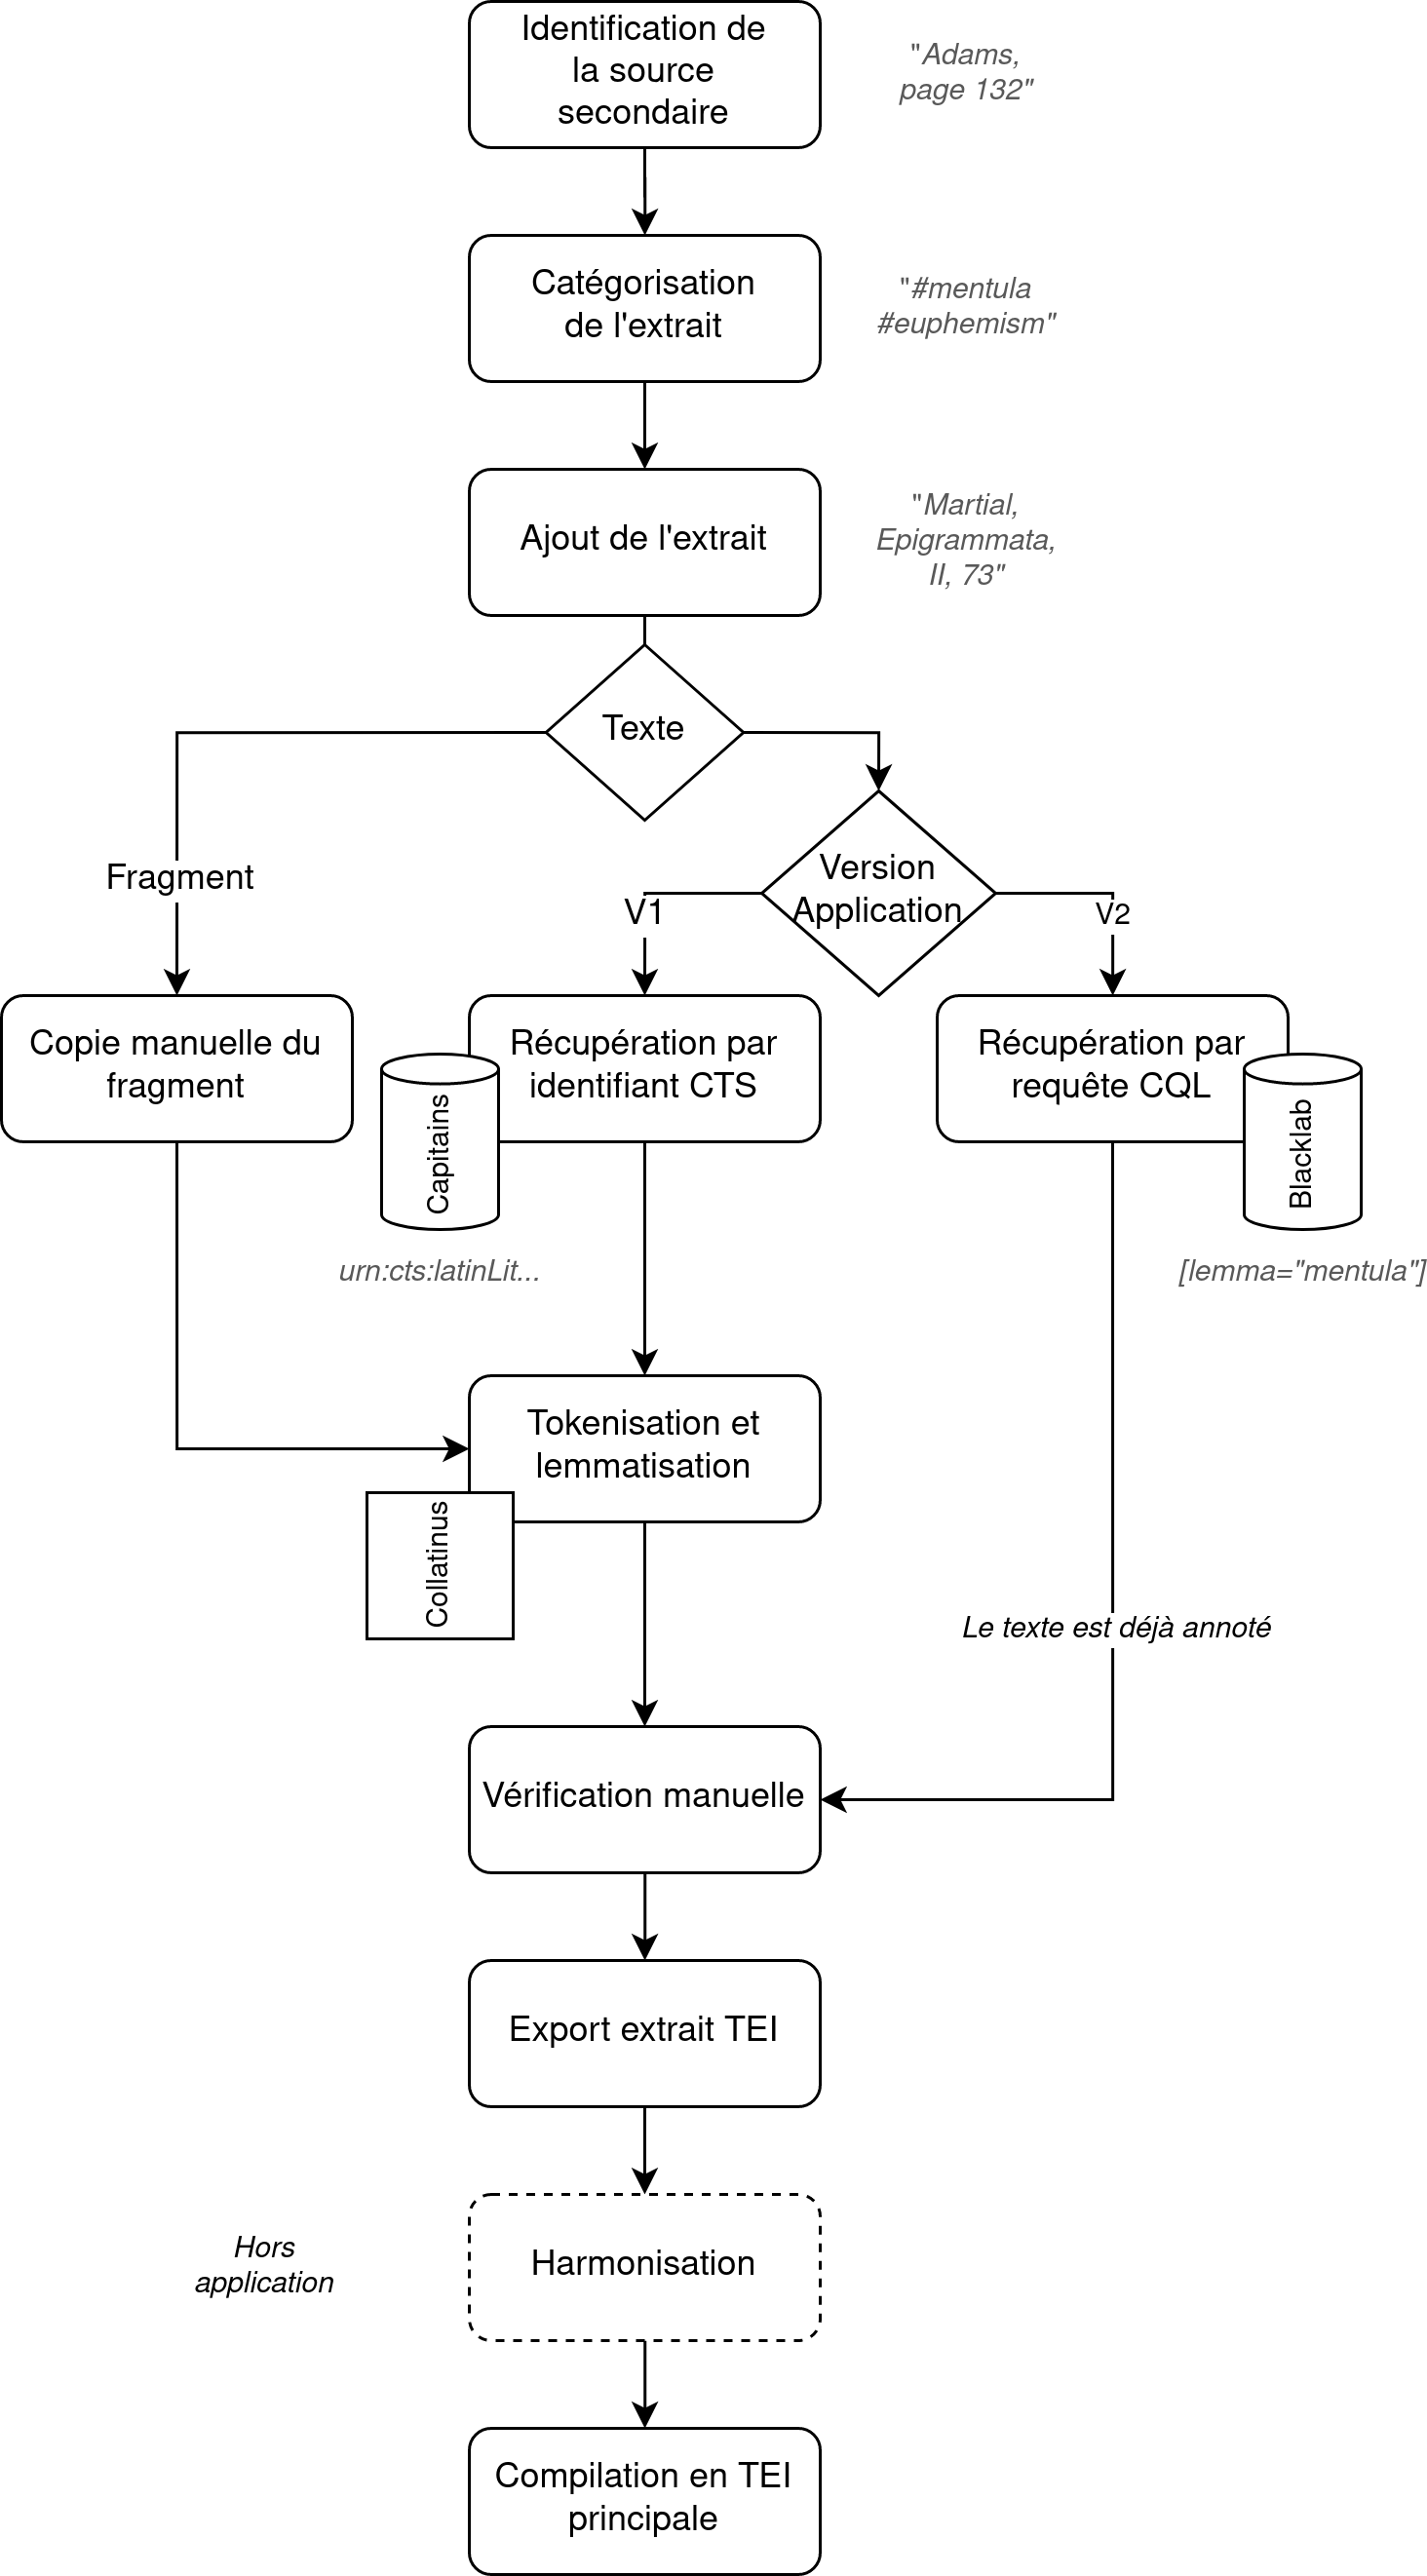
\includegraphics[width=0.6\textwidth]{figures/chap1/part3/exemplier/corpus_builder_workflow.png}
    \caption{Étapes et source des données ou annotations dans le processus de création d'exemples.}
    \label{fig:chap1:corpus_builder_workflow}
\end{figure}

Les deux versions de l'application, nommée \textit{Corpus Builder}, commencent par demander à l'utilisateur d'entrer des métadonnées concernant la source secondaire justifiant l'intégration de l'extrait: Adams et, le cas échéant, le TLL (\textit{cf.} figure \ref{fig:chap1:corpus_builder_workflow}). Une fois ces informations bibliographiques remplies, la deuxième étape est d'ajouter ou de sélectionner des catégories, utilisées alors comme mots clefs. Il est possible de les sélectionner à partir d'une base prédéfinie de mots clefs importants, de reprendre ceux retrouvés dans les extraits déjà annotés ou bien d'en ajouter de nouveaux. Une de ces annotations sort du lot: \enquote{composite} permet d'indiquer que le sens sexuel est obtenu à travers la combinaison de deux mots ou plus, par exemple \textit{cum + \_ + esse} (être avec quelqu'un)\footnote{Exemple 1466: \enquote{\textit{Quid ego tibi deliqui, si, cui nupta sum, tecum {tecum} fui ?}} \textcite[p.~177]{adams}}. Ces deux étapes permettent de préparer le document à produire du point de vue de ses métadonnées.

\begin{figure}
    \centering
    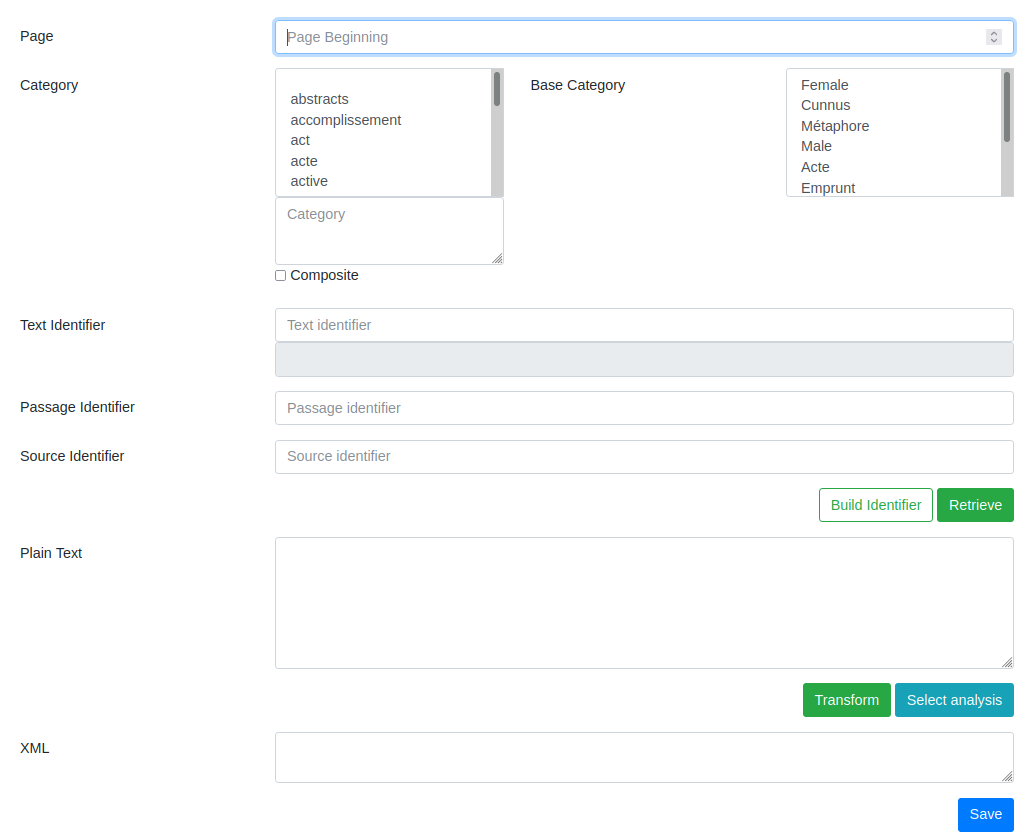
\includegraphics[width=\textwidth]{figures/chap1/part3/exemplier/corpus_builder_single.png}
    \caption{Page de l'application \textit{Corpus Builder} pour un passage unique.}
    \label{fig:chap1:corpus_builder_single}
\end{figure}

La première version de l'application (Figure \ref{fig:chap1:corpus_builder_single}), ne contenait qu'un simple système permettant soit de récupérer le texte à partir d'un identifiant CTS dans la base du meta-corpus, soit de fournir un texte \enquote{nu}, par exemple pour les fragments absents de notre compilation. Le texte est alors accompagné de métadonnées fournies par l'utilisateur: identifiant de l'oeuvre, voire de l'édition, et identifiant du passage. Une fois le texte obtenu, il est découpé en \enquote{mots}, via des règles extrêmement simples (ponctuations et espaces), et envoyées à la lemmatisation et à l'analyse morphologique à une version python de collatinus. Une fois l'analyse effectuée, une version temporaire du XML est présentée à l'utilisateur, qui peut sélectionner le ou les mots qui portent l'analyse fournie par Adams, afin de porter au niveau mot l'interprétation d'Adams via l'attribut \texttt{@ana}. L'utilisateur peut ensuite sauvegarder le document.

\begin{figure}
    \centering
    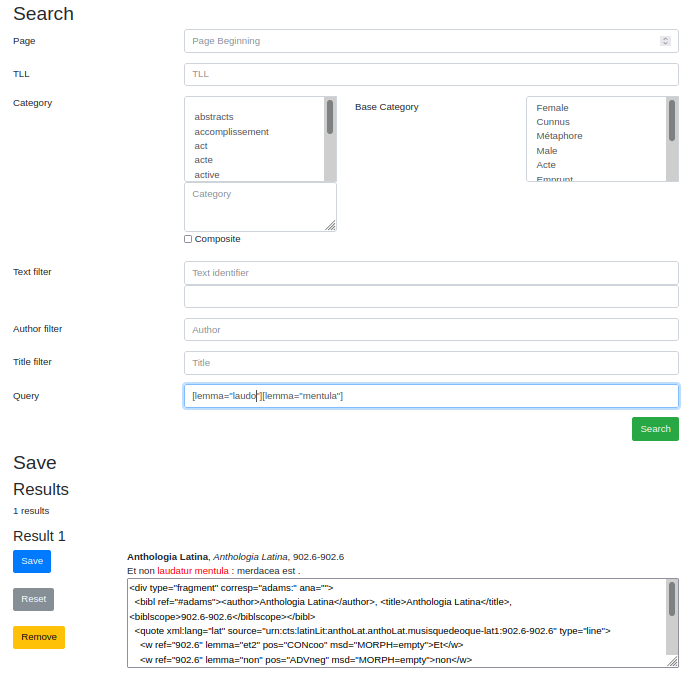
\includegraphics[width=\textwidth]{figures/chap1/part3/exemplier/corpus_builder_multiple.png}
    \caption{Page de l'application \textit{Corpus Builder} pour de multiples passages.}
    \label{fig:chap1:corpus_builder_mult}
\end{figure}

La seconde version de l'application ajoute une page de recherche multiple (Figure \ref{fig:chap1:corpus_builder_mult}). Elle repose sur une version du corpus ingérée par le moteur de recherche linguistique Blacklab\footcite{de2017creating} qui propose une interface machine (API) acceptant les requêtes utilisant le \acrfull{CQL}. Le \acrshort{CQL}\footcite{christ1994modular} est un langage de requêtage permettant de chercher des informations sur des annotations au niveau mot. Notre meta-corpus est proposé dans ce moteur de recherche sous une forme favorisant des recherches avancées (\textit{cf.} figure \ref{fig:chap1:armavirumque}): chaque mot est accompagné d'une part des annotations issues de l'extraction de données comme la structuration logique et la référence canonique du passage, et d'autre part d'annotations automatiques effectuées par le lemmatiseur Pie\footnote{\textit{Cf. Chapitre 3.}} incluant le lemme, la POS, la morphologie. On peut alors produire des requêtes complexes, s'appuyant à la fois sur les informations bibliographiques (à travers les filtres Auteur ou Oeuvre par exemple, mais aussi les filtres au niveau mot pour les passages) et sur les informations linguistiques issues de l'annotation automatique. Cette deuxième version a permis une nette accélération dans la constitution du corpus: il devenait possible d'annoter, après vérification manuelle, des dizaines d'extraits à travers une seule recherche \enquote{complexe}. Cette option est devenue d'autant plus pratique pour les situations où Adams, par manque d'espace, se contente de dire qu'il y a X occurrences d'un certain lemme chez un ou plusieurs auteurs nommés.

\begin{figure}
    \begin{lstlisting}[language=XML]
<ab type="line" n="urn:cts:latinLit:phi0690.phi003.perseus-lat2:1.1">
    <w rend="line" n="1.1" pos="NOMcom" msd="Case=Acc|Numb=Plur" lemma="arma">Arma</w>
    <w rend="line" n="1.1" pos="NOMcom" msd="Case=Acc|Numb=Sing" lemma="uir">virumque</w>
    <w rend="line" n="1.1" pos="CON" msd="MORPH=empty" lemma="que">{virumque}</w>
    <w rend="line" n="1.1" pos="ADJqua" msd="Numb=Sing|Gend=MascNeut|Deg=Pos|Mood=Ind|Tense=Pres|Voice=Act|Person=1" lemma="cano">cano</w>
    <w rend="line" n="1.1" pos="PUNC" msd="MORPH=empty" lemma=",">,</w>
    \end{lstlisting}
    \caption{Premiers mots de l'\textit{Énéide} de Virgile dans le document ingéré par Blacklab.}
    \label{fig:chap1:armavirumque}
\end{figure}

La lemmatisation issue de la première version et donc de l'outil \textit{Collatinus}\footnote{Décrit en chapitre 3.} a été complètement reprise une fois la compilation des documents achevée. Afin de proposer une version cohérente des données pour l'apprentissage machine, chaque mot a été annoté par le même lemmatiseur que celui utilisé pour le meta-corpus dans Blacklab, ajoutant ainsi un lemme, une POS et une analyse morpho-syntaxique. Enfin, les mots-clefs dérivés des catégories d'Adams ont été harmonisés, semi-automatiquement: les listes n'étaient pas assez contraignantes et des variations orthographiques s'étaient glissées. Nettoyer ces données permettait ainsi d'optimiser l'opérabilité de ces dernières dans un exemplier désormais cohérent en interne.

% Interpréter Adams: le problème des tags ?
% Notes sur quelques données absentes

\subsubsection{Produit final: navigation et analyse quantitative}

Après avoir produit d'abord un meta-corpus important et finement structuré, nous avons pu produire, à travers un ensemble d'outils que nous avons précédemment présentés, un exemplier numérique. Nous proposons, avant d'aller plus loin dans le traitement numérique de cet exemplier (Chapitre 5), de décrire cette base de données nouvelles, puis de décrire comment, à l'aide d'une interface développée pour l'occasion et en plus de sa mise à disposition en XML TEI, nous mettons à disposition ces données.

\paragraph{Caractéristiques statistiques de l'exemplier}

L'exemplier produit est massif: deux mille cinq cent seize exemples le composent. Il comprend 38~201 mots (hors ponctuation) répartis entre quatre-vingt-dix-sept auteurs. Il est composé de cent quatre-vingt-dix-neuf catégories ou tags, utilisés dans huit mille deux cent quinze annotations pour trois centre quarante deux combinaisons uniques. Le set de données s'étend de Plaute (-254) à Pierre Diacre (1159): le texte de ce dernier a été inclus suite à une erreur de datation, la date la plus tardive serait plutôt le premier Mythographe du Vatican. Ce dernier a été daté pendant longtemps autour des V\textsuperscript{e} et VI\textsuperscript{e}, ce qui justifie son inclusion, mais cette datation est fortement remise en cause dans sa dernière édition de 1995\footnote{D'après le projet DigilibLT, \textcite{zorzetti_premier_1995}.}, où Nevio Zorzetti et Jacques Berlioz proposent une datation entre le VIII\textsuperscript{e} et le IX\textsuperscript{e} siècle.

\begin{figure}
    \centering
    \begin{minipage}[b]{.48\linewidth}%
        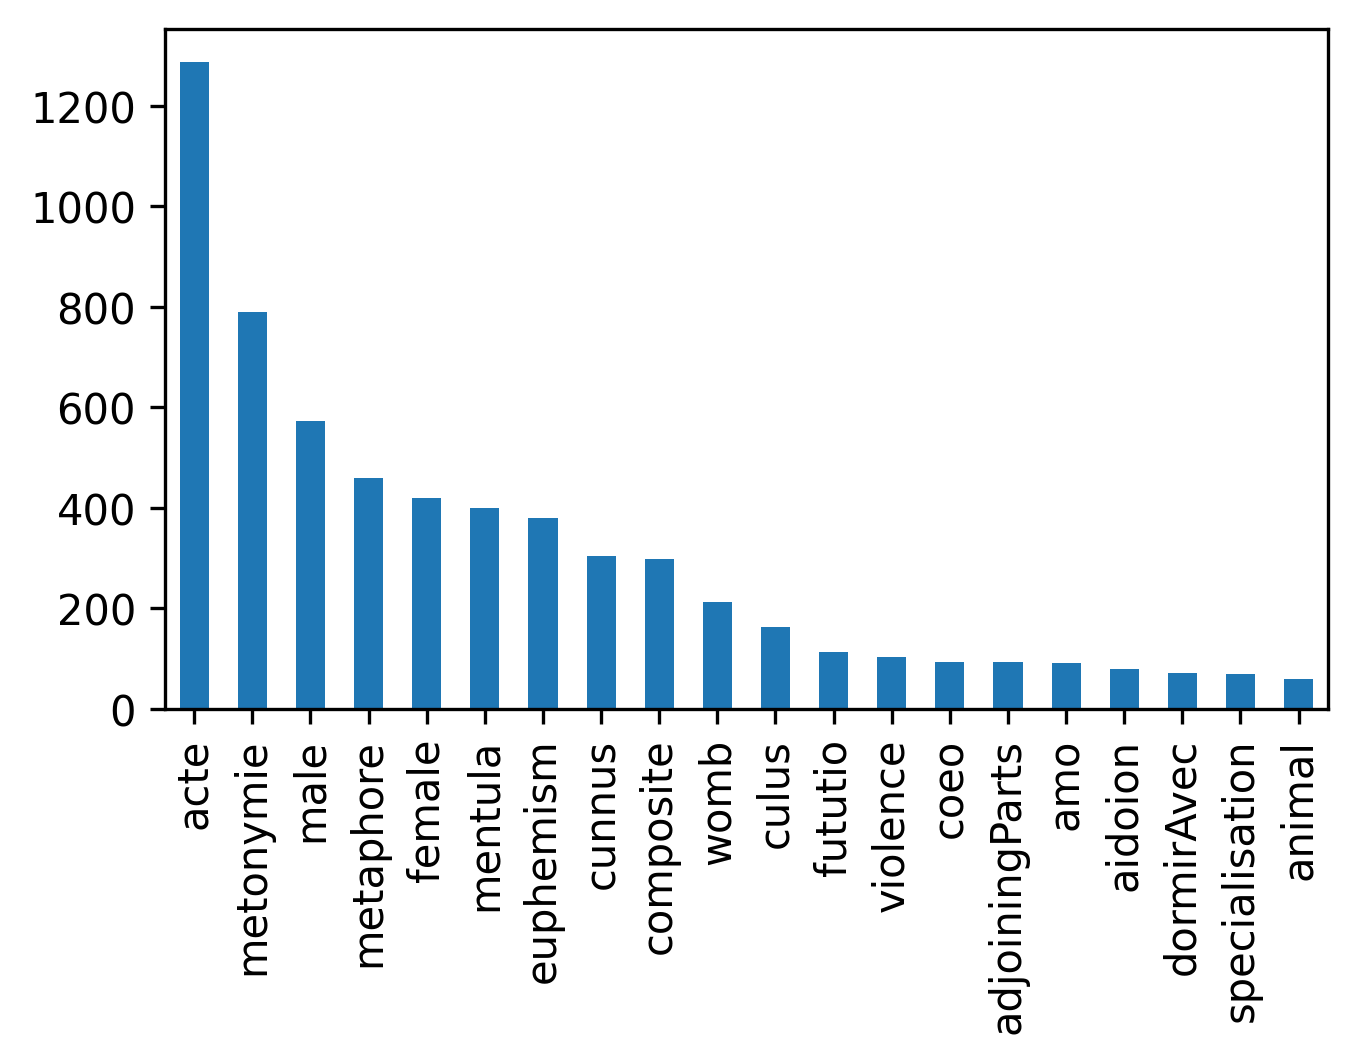
\includegraphics[width=\linewidth]{figures/chap1/part3/exemplier/tags.png}
        \caption{Vingt tags les plus fréquents de l'exemplier}
        \label{fig:chap1:tag_mostfrequents}
    \end{minipage}
    \hfill
    \begin{minipage}[b]{.48\linewidth}%
        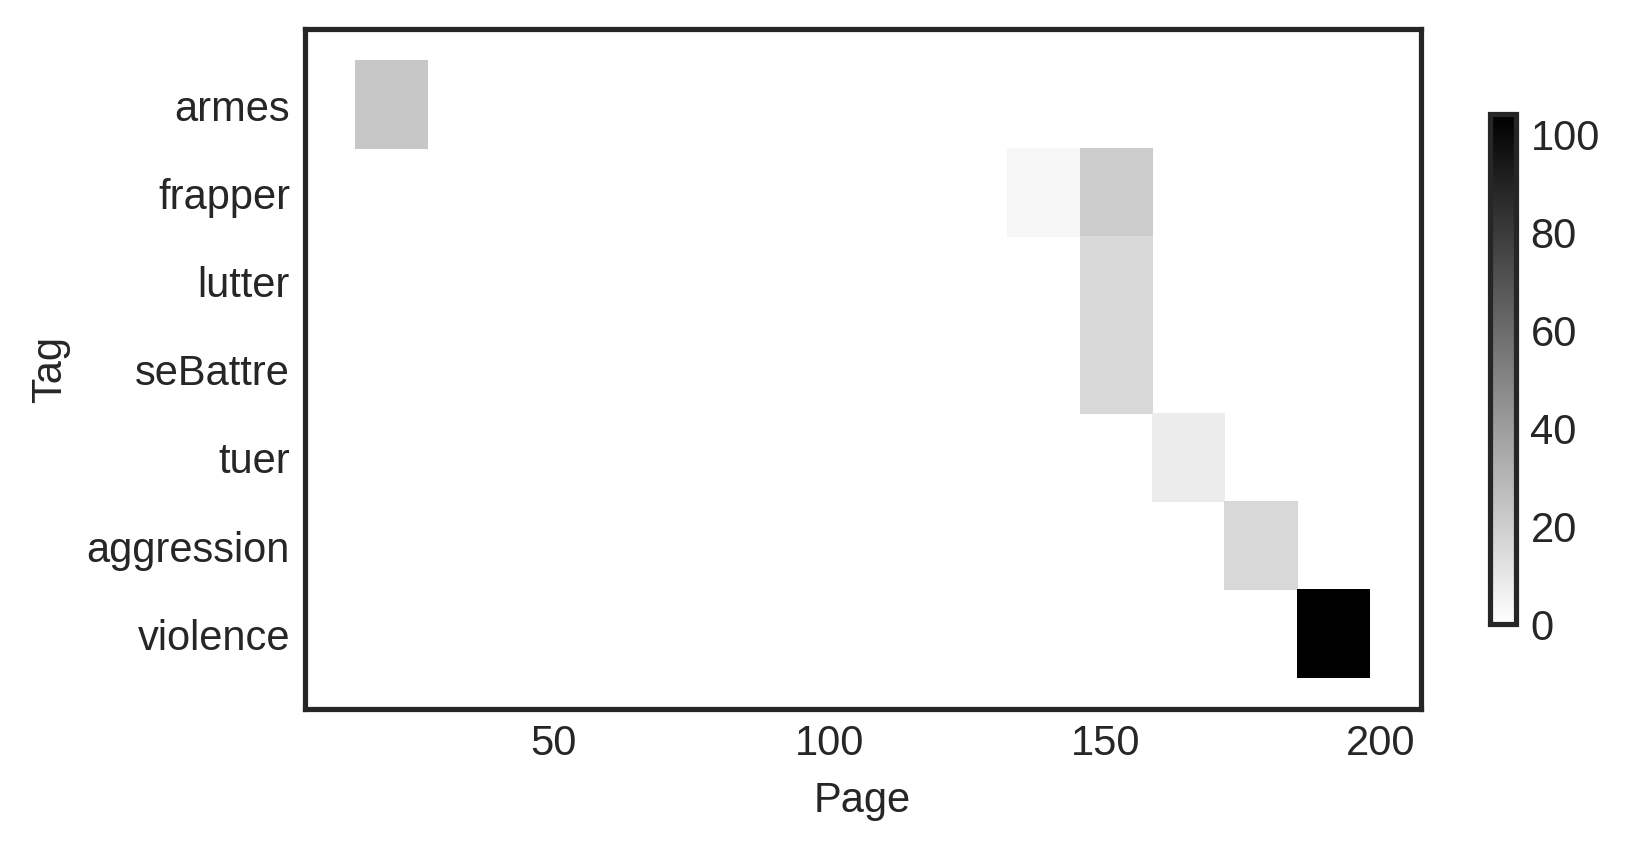
\includegraphics[width=\linewidth]{figures/chap1/part3/exemplier/violence.png}
        \caption{Fréquence des tags liés à la violence}
        \label{fig:chap1:tags_violence}
    \end{minipage}
\end{figure}

Les annotations catégorielles les plus communes sont sans surprise les catégories principales d'Adams, avec d'une part les catégories \enquote{thématiques} (ses chapitres: acte, \textit{male} pour sexe masculin, \textit{female} pour sexe féminin, \textit{culus}) et ses outils d'analyse intra-thématiques (\textit{metaphore}, \textit{metonymie)}. En figure \ref{fig:chap1:tag_mostfrequents}, ces vingts tags réservent tout de même quelques surprises, notamment celui \enquote{animal} qui recouvre métaphores animales ou vocabulaire appliqué aux animaux. 

Cette visualisation met en exergue les aspects critiquables de ces catégorisations\footnote{Si cette erreur de méthode ne met pas en valeur notre travail, il nous semble capital d'en informer les différents utilisateurs, car elle pourrait bien induire des erreurs d'interprétations.}. Par exemple, le mot clef \enquote{violence} a été utilisé lorsqu'Adams a spécifié clairement qu'un déploiement lexical était violent. Si l'on regarde la figure \ref{fig:chap1:tags_violence}, il est clair que la lecture linéaire d'Adams, sans savoir en amont l'ensemble des catégories ou qualifications qui sont utilisées par adams, a produit en aval des traitements différenciés de ces dernières. C'est une faiblesse notable de l'usage des catégorisations, en dehors des catégories extrêmement claires de l'auteur lui-même (type \enquote{acte} et \enquote{métaphores}). En cas d'introduction d'exemples à travers d'autres sources secondaires comme celles d'Amy Richlin, il sera nécessaire de lisser ces catégories et de décrire l'ontologie de classement proposée. Cette solidification des fondamentaux est essentielle. Cet élargissement et approfondissement de l'ontologie devrait inclure aussi une meilleure qualification des acteurs des actes et des sens de l'acte. Des catégories telles que \texttt{\#Actif:Homme}, \texttt{\#Actif:Esclave}, etc. permettraient, y compris à travers des approches modernes et potentiellement anachroniques, de réinterroger ces dernières.

\begin{figure}[ht]
    \centering
    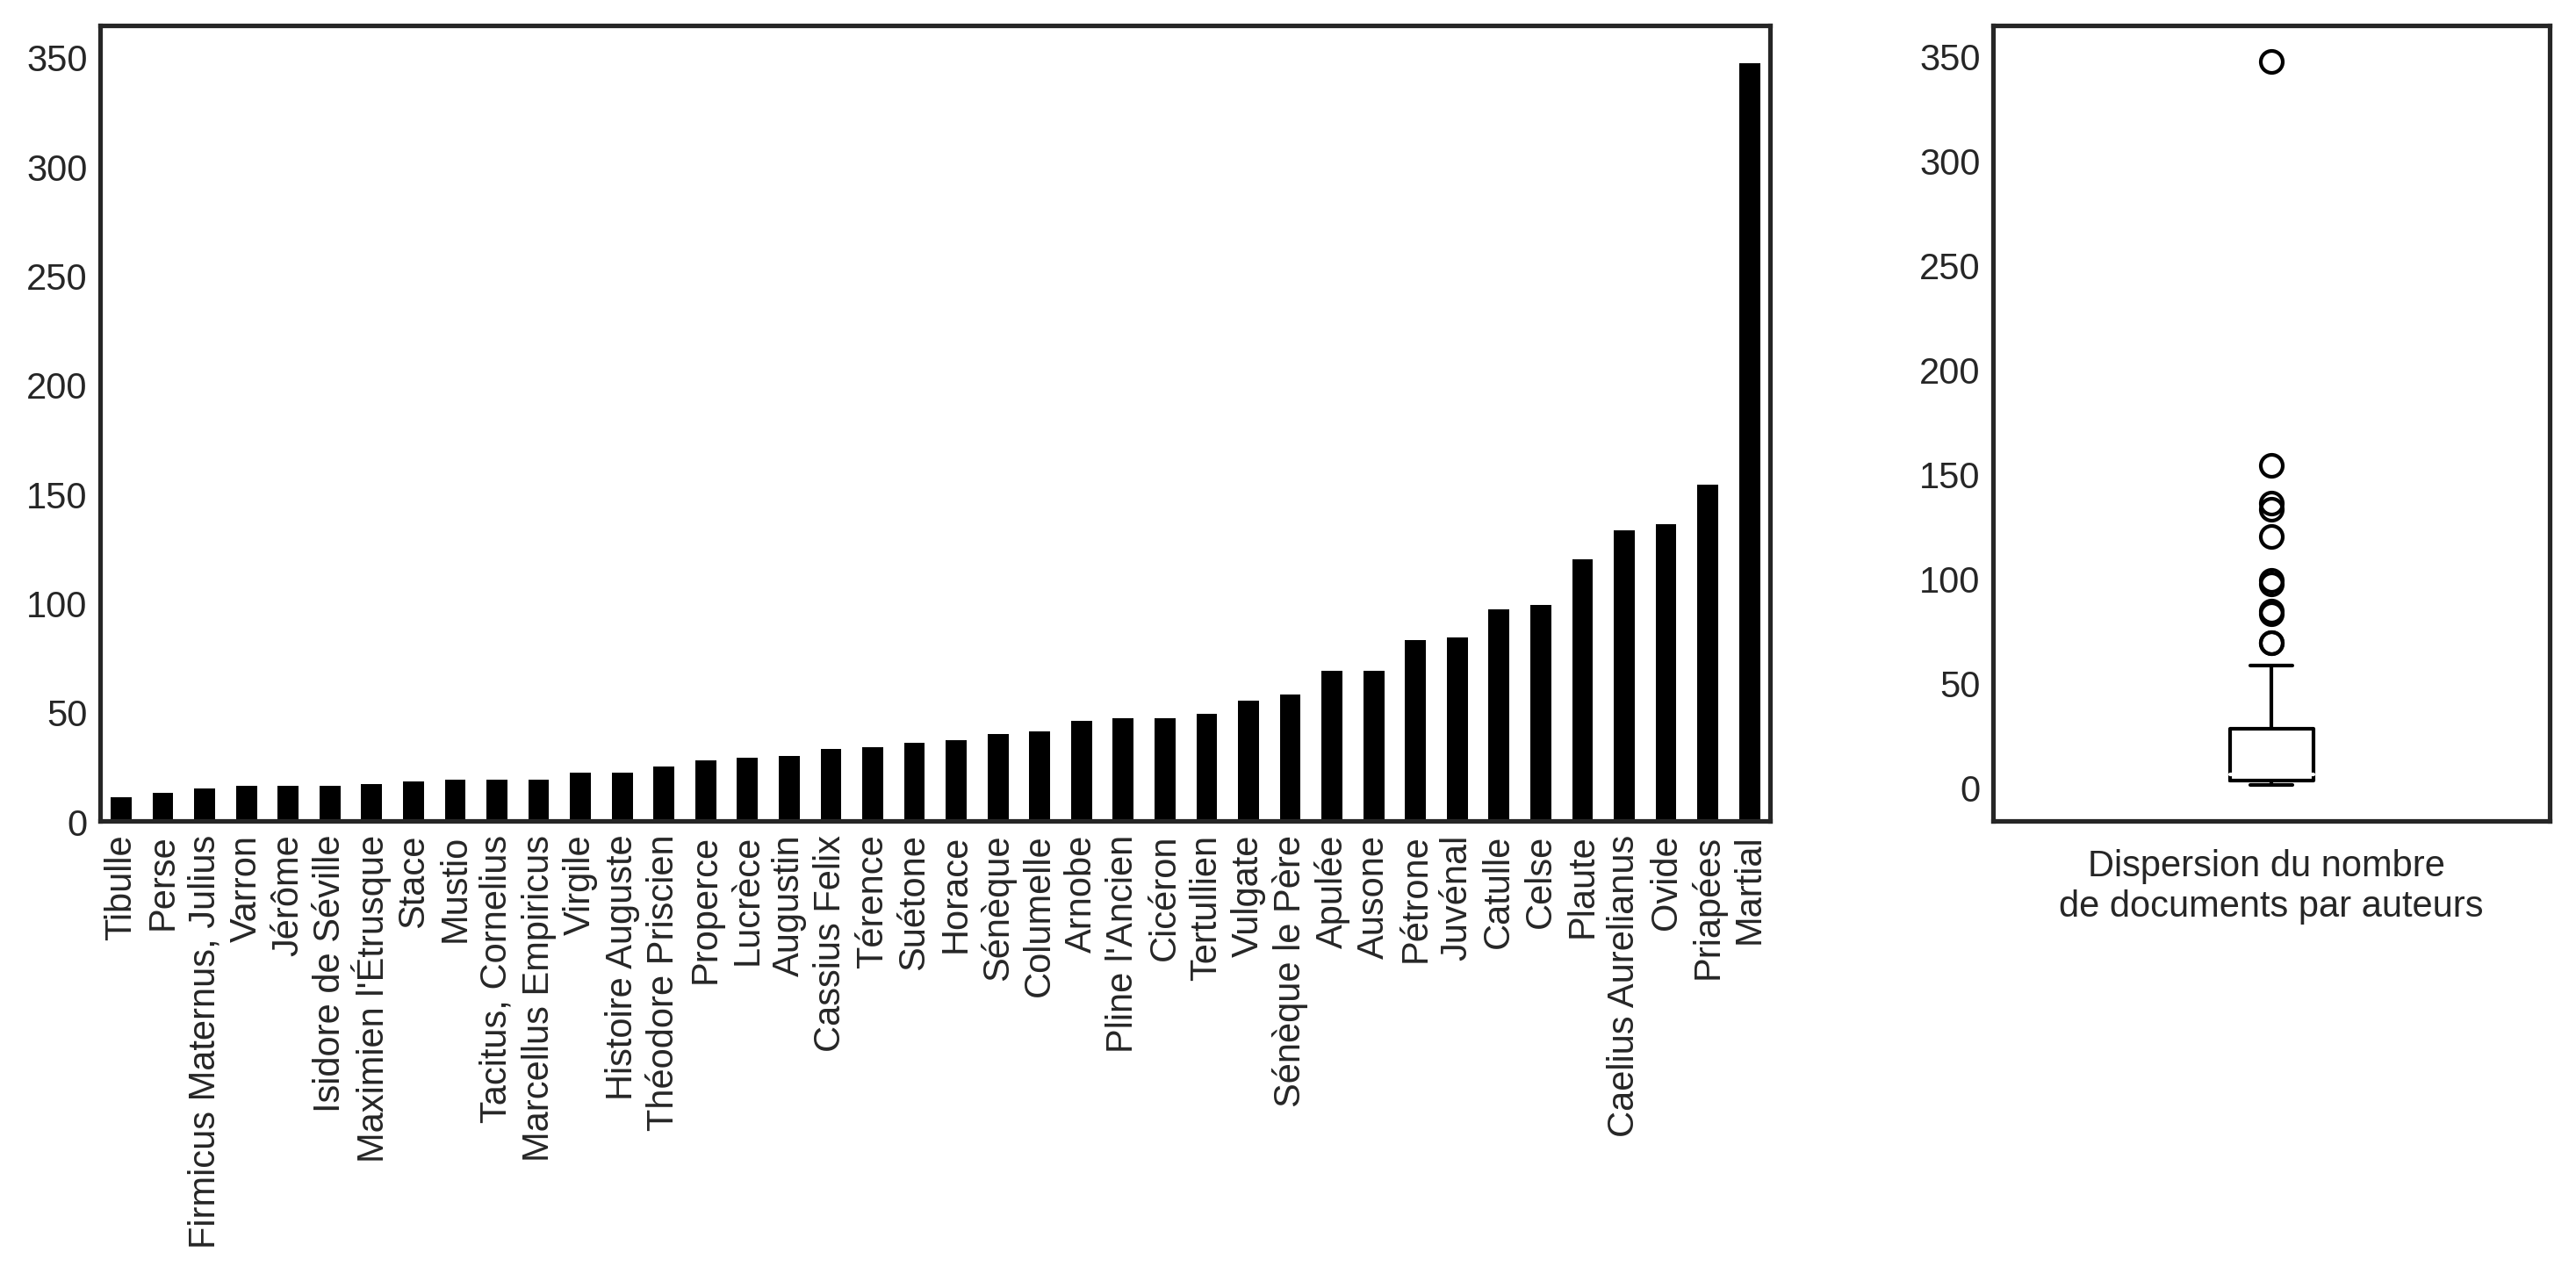
\includegraphics[width=\linewidth]{figures/chap1/part3/exemplier/auteurs_exemplier_absolus.png}
    \caption{Auteurs les plus importants en nombre d'exemples.}
    \label{fig:chap1:nb_extraits_auteur}
    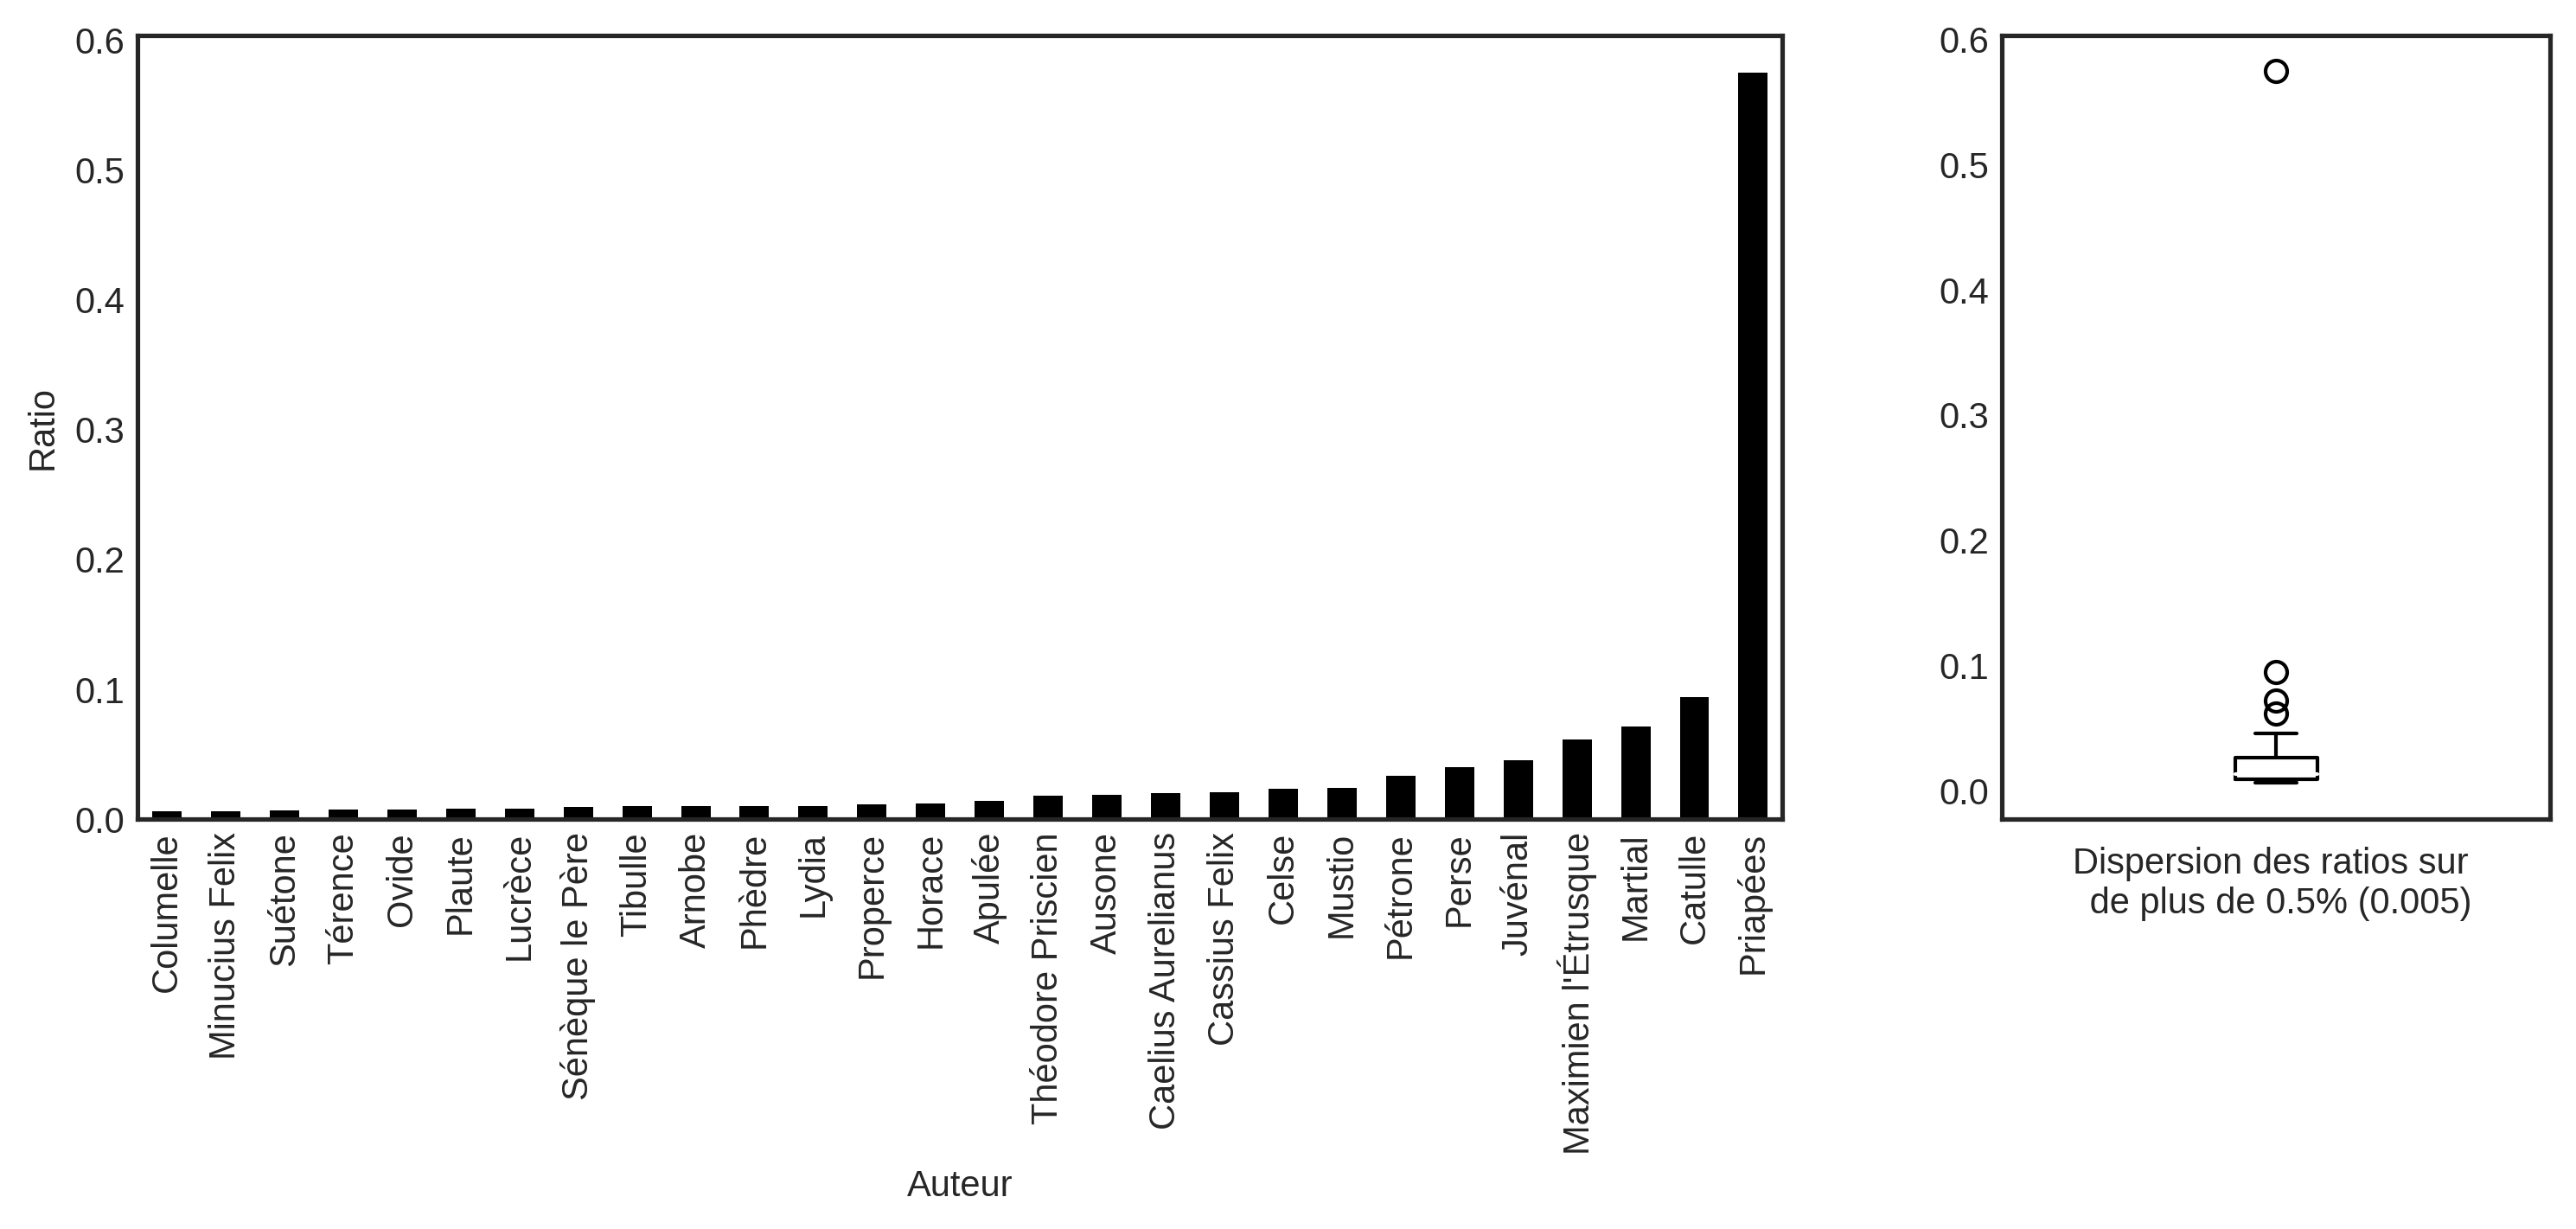
\includegraphics[width=\linewidth]{figures/chap1/part3/exemplier/auteurs_exemplier_motsrelatifs.png}
    \caption{Auteurs les plus importants en fonction du ratio Nombre de mots dans l'exemplier par nombre de mots dans le meta-corpus.}
    \label{fig:chap1:nb_extraits_auteur_rel}
\end{figure}

La distribution des exemples en fonction de leur auteur ou de la compilation qui les contient montre une distribution logique (peu d'auteurs sont extrêmement riches en exemples) et générique. Les auteurs les plus importants du corpus en nombre d'exemples sont des poètes (Ovide, Catulle, Martial, etc.), des médecins ou \enquote{scientifiques} (Caellius Aurelianus, Celse) ou des auteurs de comédie (Plaute). Martial est en valeur absolue l'auteur le plus prolifique d'exemple dans notre corpus: son langage fleuri et les thèmes qu'il aborde en font un auteur incontournable pour la compréhension de la sexualité latine. Mais, ce chiffrage absolu mis en regard de la taille de l'oeuvre de chaque auteur (\textit{cf.} figure \ref{fig:chap1:nb_extraits_auteur_rel}),  donne une image différente de certains auteurs. Par exemple, Catulle, en septième place en quantité d'exemples, se retrouve en deuxième place dans cette manière d'aborder le corpus. Cela signifie que, comparé à Martial, Catulle parle plus souvent de sexualité par mots qu'il écrit. Ces chiffres montrent aussi la spécificité de l'écriture des Priapées, avec plus d'un mot sur deux écrits repris dans l'exemplier. Ils soulignent aussi celle des médecins ou gynécologues comme Celse ou Mustio, qui se glisse dans les dix auteurs les plus prolifiques par mot écrit. Enfin, il met en lumière des phénomènes de transmission, comme pour Maximien l'Étrusque, que l'on ne connait que pour six élégies, et qui, mécaniquement, se retrouve en haut des scores (4~300~mots).

\afterpage{%
\begin{sidewaysfigure}%
    \centering
    \begin{subfigure}{0.45\hsize}
        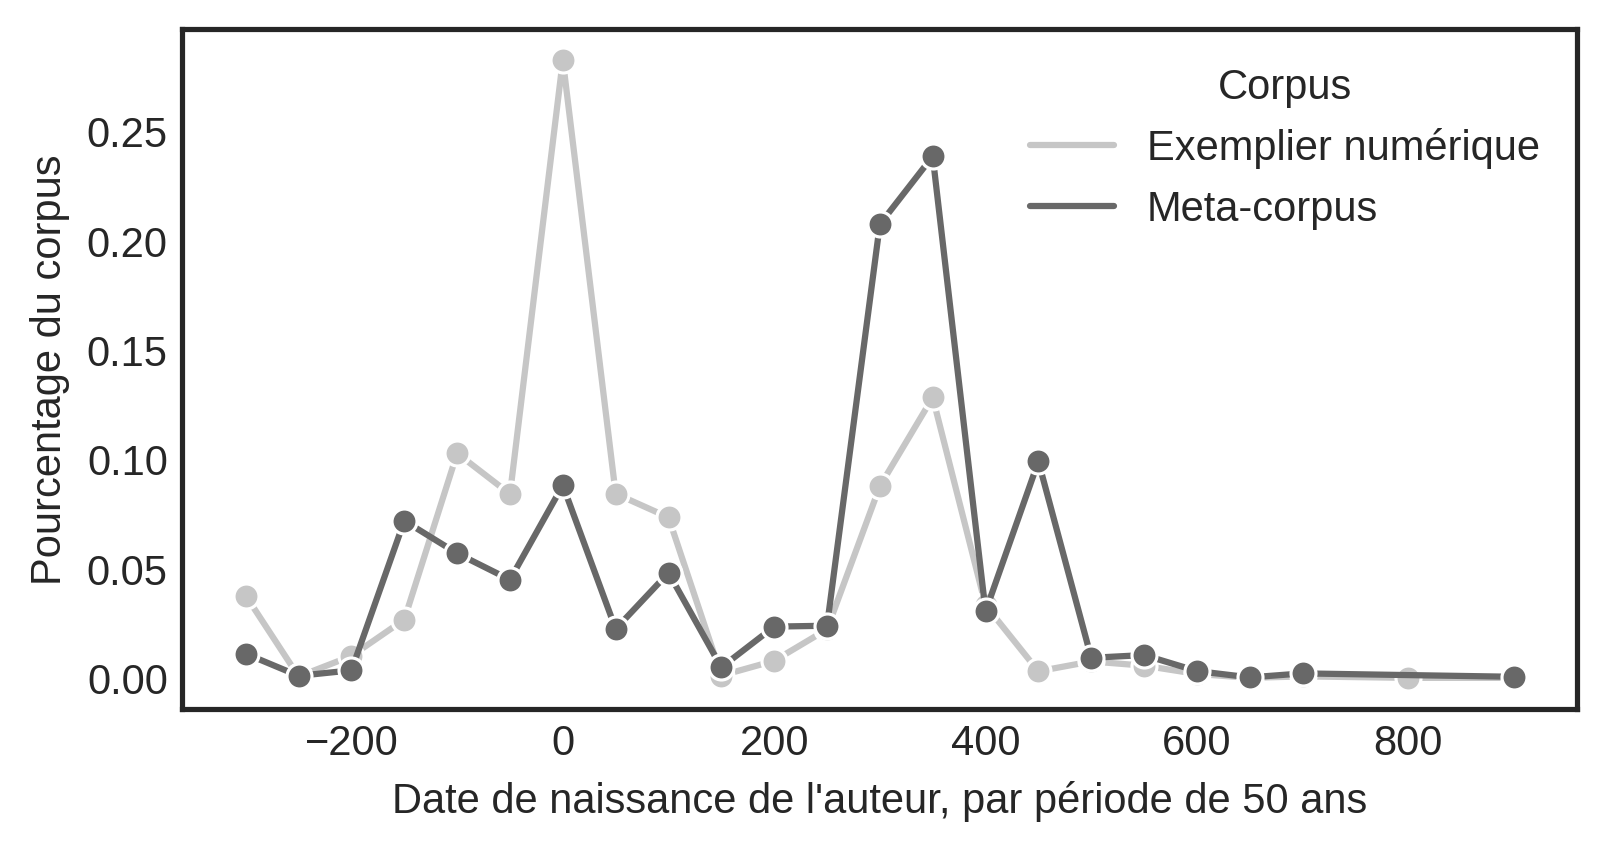
\includegraphics[width=\linewidth]{figures/chap1/part3/exemplier/evol_brut_exemplier.png}
        \caption{Répartitions des parts des corpus par date de naissance des auteurs. La période 0--50, incluant Martial, représente 25\% des extraits de l'exemplier.}
        \label{fig:chap1:exemplierdatation:brut_percent}
    \end{subfigure}%
    \hfill
    \begin{subfigure}{0.45\hsize}
        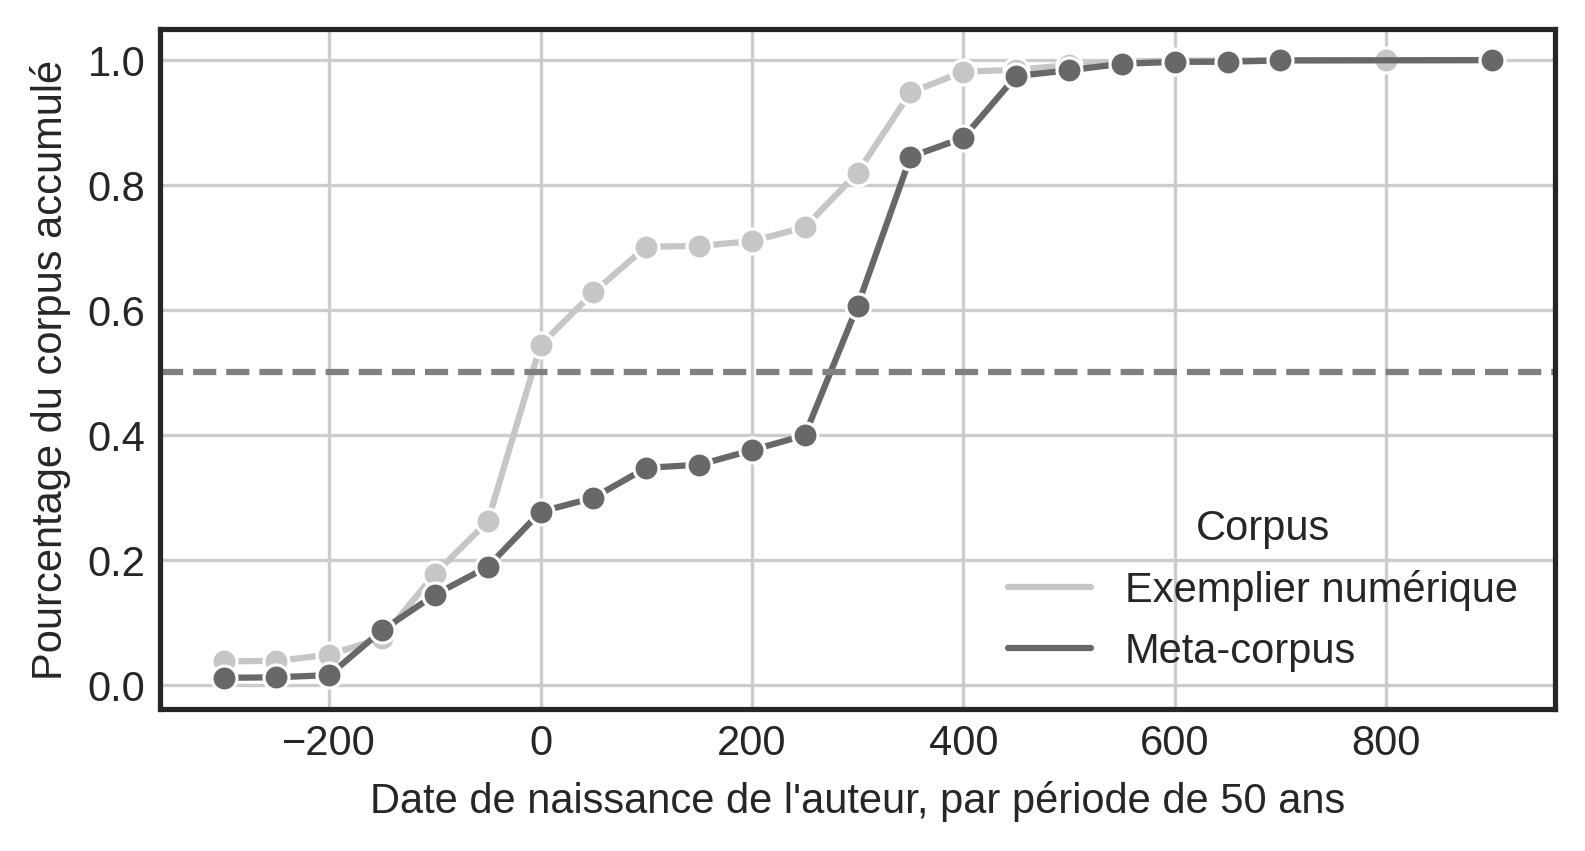
\includegraphics[width=\linewidth]{figures/chap1/part3/exemplier/evol_accumul_exemplier.png}
        \caption{Accumulation des parts des corpus par date de naissance des auteurs. La période 0--50 représente le dépassement de la barre des 50\% de l'exemplier.}
        \label{fig:chap1:exemplierdatation:accumul_percent}
    \end{subfigure}%
    \\
    \begin{subfigure}{0.45\hsize}
        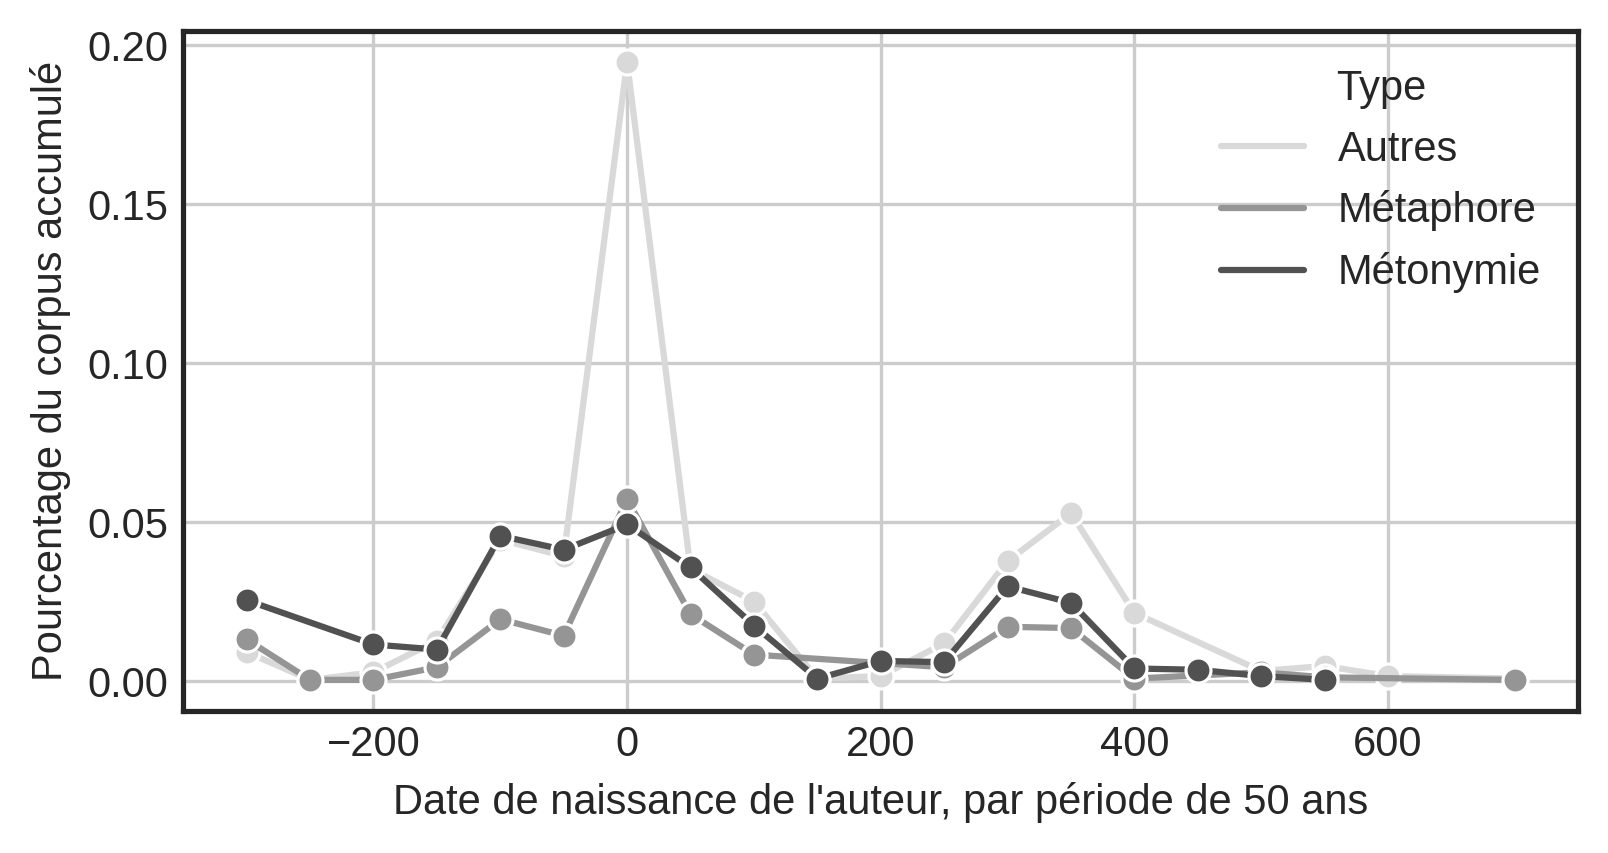
\includegraphics[width=\linewidth]{figures/chap1/part3/exemplier/evol_tags_exemplier.png}
        \caption{Répartitions des grands sous-types d'Adams (en pourcentage du corpus total) par date de naissance des auteurs. La période 0-50 a 20\% d'extraits qui ne sont ni des métaphores ni des métonymies.}
        \label{fig:chap1:exemplierdatation:tags}
    \end{subfigure}%
    \hfill
    \begin{subfigure}{0.45\hsize}
        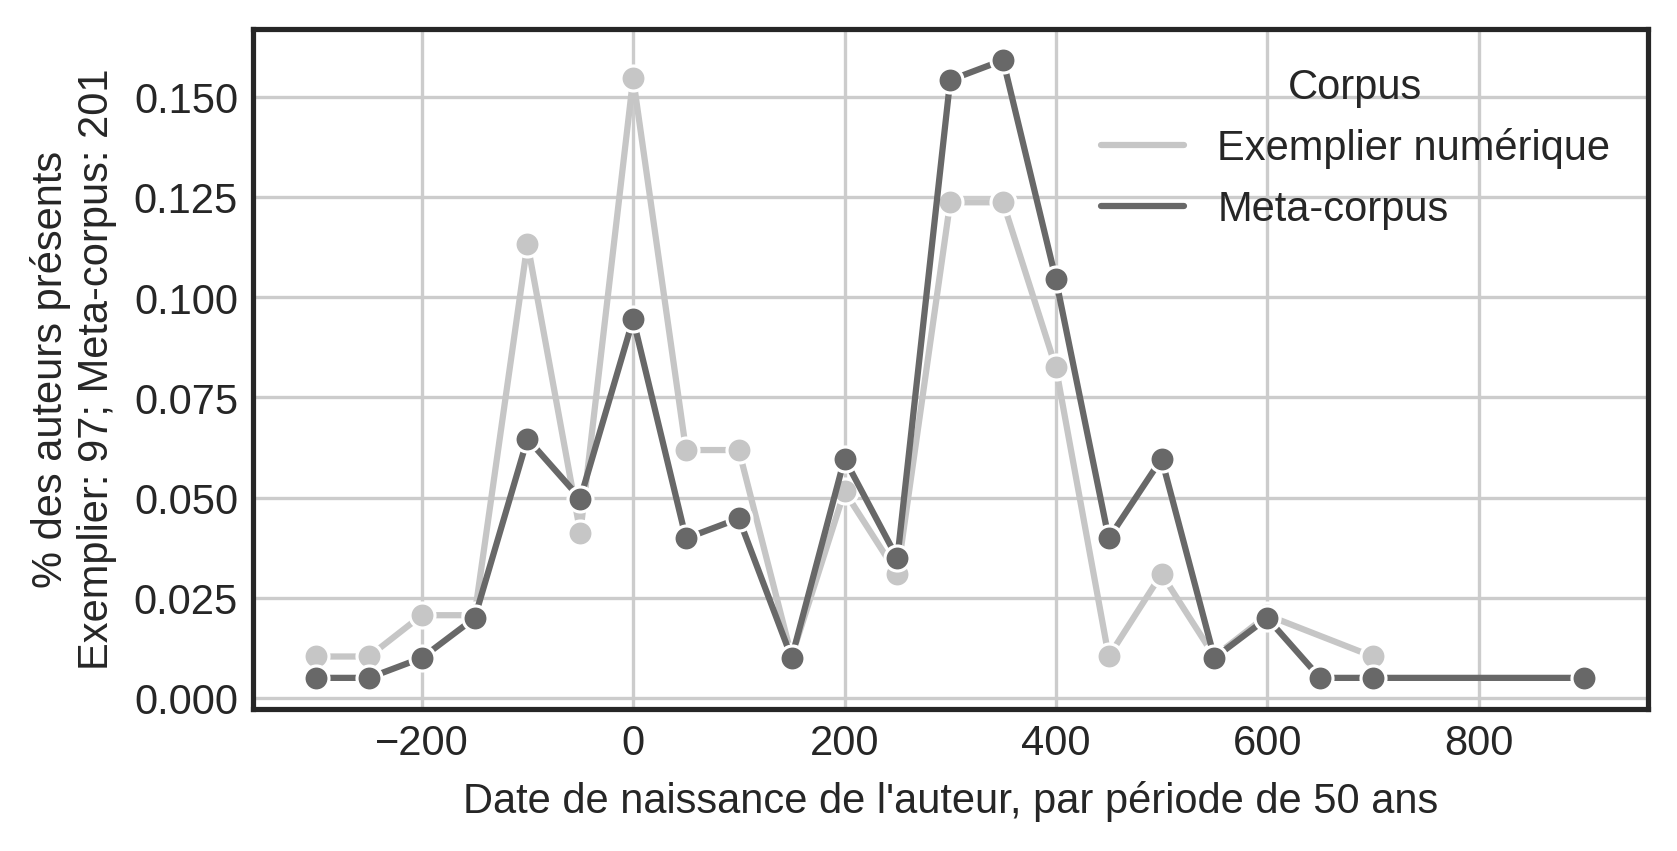
\includegraphics[width=\linewidth]{figures/chap1/part3/exemplier/evol_auteurs_exemplier.png}
        \caption{Répartitions de la portion des auteurs connus des corpus par date de naissance des auteurs. La période 0-50 contient 15\% des auteurs de l'exemplier numérique.}
        \label{fig:chap1:exemplierdatation:auteurs}
    \end{subfigure}%
    \caption{Évolution de l'exemplier en fonction de la date de naissance de l'auteur.}
    \label{fig:chap1:exemplierdatation}
\end{sidewaysfigure}%
\clearpage
}
% Chronologie

La répartition chronologique des exemples permet d'appuyer quelques points vus à propos du méta-corpus (\textit{cf.} figure \ref{fig:chap1:exemplierdatation}). Deux pics forment le corpus: l'un au début de l'Empire et l'un à l'apparition des oeuvres des Pères latins de l'Église. Mais la force de ces pics est inversée. Quand le meta-corpus atteint son plus fort pic autour de 300 avec près de 25\% de sa couverture en nombre de mots à cette époque (\textit{cf.} figure \ref{fig:chap1:exemplierdatation:brut_percent}), l'exemplier numérique contient entre 0 et 50 plus de 25\% des siens. Les auteurs de l'exemplier nés entre 0 et 50 et ou les oeuvres qui sont datées à partir de cette intervalle ne sont pas n'importe qui: Martial (Premier auteur le plus important en nombre d'exemples), Celse (Sixième), Pline l'Ancien (Seizième), l'\textit{Anthologie Latine} et les \textit{Priapées} (Deuxième). Cet écart entre période chrétienne et période classique, qui commence à se former dès la naissance des élégiaques entre -100 et 0, est clairement visible en figure \ref{fig:chap1:exemplierdatation:accumul_percent}: l'exemplier atteint la moitié de sa taille entre 0 et 50, 75\% entre 100 et 150 là où le meta-corpus n'atteind ces chiffres qu'entre 250 et 350.

Pour autant, parle-t-on moins de sexualité à la période Chrétienne ? Il nous semble deux hypothèses peuvent être avancées:
\begin{enumerate}
    \item Adams se sert beaucoup du TLL pour traiter de la période tardive et chrétienne, et le TLL pourrait avoir un traitement plus faible de cette même période. Leur couverture des textes médicaux étant imparfaite, une autre part du corpus tardif est ignoré.
    \item L'antiquité tardive ne parle pas ou plus de sexe, soit par changement générique (moins de satire, moins de poésie érotique), soit par sélection dans la transmission des textes.
\end{enumerate}

Il s'agit plus que probablement d'une combinaison de ces deux hypothèses. Il est sûr qu'Adams traite moins la période tardive, les compte-rendus font clairement mention de ce manque. Alan D. Booth reproche à Adams d'avoir assez peu couvert la période chrétienne (\enquote{les incursions dans le latin médiéval auraient pu être remplacées par un examen du vocabulaire sexuel et des attitudes chez les premiers auteurs Chrétiens\footcite{booth_adams}}) tandis qu'Aline Rousselle lui reproche l'\enquote{absence [partielle] de paragraphe purement médical, anatomique}. Il est clair en tout cas, au regard de l'emploi des auteurs disponibles (\textit{cf.} figure \ref{fig:chap1:exemplierdatation:auteurs}), que les auteurs de la période tardive sont sous-exploités dans l'exemplier.

Il est aussi fort probable que les textes qui nous sont parvenus sur la sexualité soient devenus plus rares ou aient changé de forme, soit par l'effet de sélection dans la transmission soit à cause du changement culturel que représente en partie la période chrétienne. Il est sûr que la poésie galante ou érotique est moins présente, à notre connaissance, au IV\textsuperscript{e} qu'au I\textsuperscript{er} siècle de notre ère. Mais pour autant, l'isotopie de la sexualité disparaît-elle dans une religion qui s'est fait connaître au fil des siècles pour son contrôle des corps ? Il nous semble plus juste de dire qu'il s'agit surtout d'un changement de ses modalités d'expressions. D'abord, à travers les changements génériques, l'obscénité se fait plus rare au IV\textsuperscript{e} siècle qu'au premier, ou du moins, l'expression de l'isotopie sexuelle par un vocabulaire sans détours y est beaucoup plus rare (\textit{cf.} figure \ref{fig:chap1:exemplierdatation:tags}). Là où les expressions imagées, qu'il s'agisse de métonymies ou de métaphores, arrivent à la période Chrétienne à des taux similaires à ceux de la période du Haut empire, la part de formes \enquote{basiques\footnote{C'est le mot qu'utilise Adams pour désigner ses premières parties de chapitre.}} est quatre fois moins importantes pendant la période tardive.
% Mots les plus fréquents ?

\begin{figure}
    \centering
    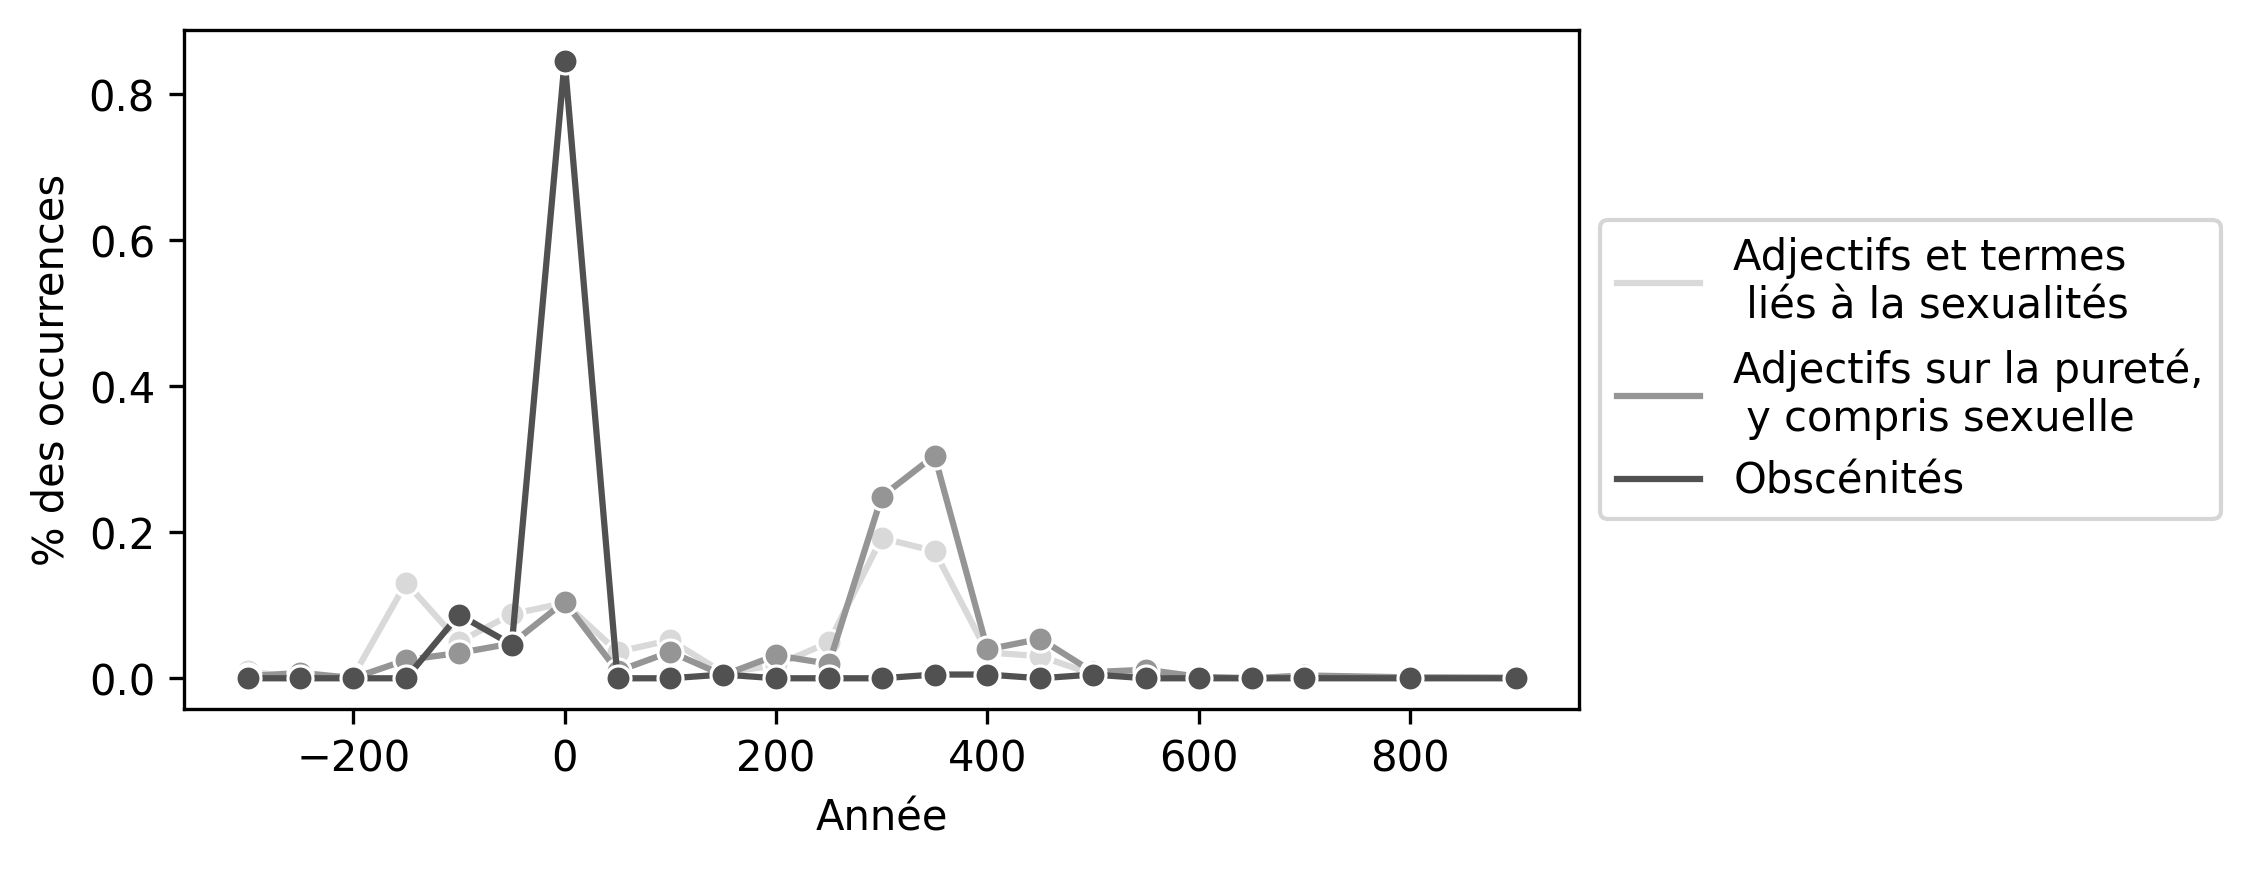
\includegraphics[width=\linewidth]{figures/chap1/part3/exemplier/exemplier_prcentage_occs.png}
    \caption{Part des occurrences de trois groupes lexicaux en fonction des années. Le groupe \textit{Obscénités} atteint 80\% de ses occurrences avec les auteurs nés entre 0 et 50.}
    \label{fig:exemplier:lexical_groups}
\end{figure}

Il ne faut pas non plus perdre de vue l'angle d'attaque d'Adams sur son livre pour expliquer cette chute. Si le IV\textsuperscript{e} siècle est beaucoup moins représenté, c'est aussi qu'il parle probablement de sexualité à travers d'autres termes, par exemple à travers des évaluations morales (\textit{lascivus}, \textit{impudicus}) ou par les louanges de l'absence de sexualité (\textit{virginitas}, \textit{puritas}). En guise d'aperçu, un regroupement autour de trois groupes lexicaux et la répartition de leurs occurrences sur le meta-corpus donne une image correspondante à cette \textit{intuition}, sans la confirmer tant certains des termes qui les composent sont complexes (\textit{cf.} figure \ref{fig:exemplier:lexical_groups}). Ces groupes lexicaux sont:
\begin{enumerate}
    \item Les \enquote{Adjectifs et termes liés à la sexualité}, soit la famille \textit{lasciv-}, \textit{mollis}, \textit{mollitia}, \textit{libido}, \textit{impurus}, \textit{voluptas}. 
    \item Les \enquote{Adjectifs et termes liés à l'absence de sexualité}, en particulier la notion de virginité: \textit{virginitas}, \textit{purus}, \textit{puritas}.
    \item Les \textit{Obscénités} les plus marquantes: \textit{mentula}, \textit{futuo}, \textit{pedico}, \textit{irrumo}, \textit{cunnus}.
\end{enumerate}

Il devient alors clair que les obscénités n'existent presque qu'à travers les auteurs nés entre -150 et 50, alors que les groupes (1) et (2), s'ils pré-existent à la période chrétienne des Pères , connaissent une explosion pendant cette période. Il ne peut s'agir ici que d'appuyer l'intuition d'un changement d'approche des discours sur la sexualité, qui n'a clairement pas été envisagé par Adams. Elle pose une question importante: la virginité fait-elle partie de l'espace sémantique de la sexualité ? Chez l'auteur du \textit{Latin Sexual Vocabulary}, il est clair qu'elle n'y fait partie que quand elle est enlevée: il n'y fait mention que dans ce contexte, qu'il s'agisse de \textit{uirginitatem eripio}\footcite[p.~195]{adams}, ou dans celui de métaphores permettant de parler du sexe féminin, telles que \textit{uirginalem scrobem}\footcite[p.~151]{adams} (cavité virginale) chez Arnobe.

Cette compilation et sa visualisation nous permettent ainsi de mettre encore une fois en lumière les forces et les faiblesses du travail d'Adams, comprenant un peu plus l'angle scientifique qu'il avait lorsqu'il avait rédigé son travail. Aline Rousselle dit dans dans son compte-rendu qu'Adams fait un \enquote{vocabulaire obscène et non, comme le dit le titre, [un] vocabulaire sexuel}\footcite{rousselle_j_1987}. Il nous semble du moins que l'auteur du \textit{Vocabulary} s'est attaché plus particulièrement à l'obscénité et à la sexualité \enquote{en cours} plutôt qu'à ce que nous appellerions peut-être de \enquote{sexualité latente} ou de \enquote{discours sur la sexualité}, où celle-ci n'est pas le centre du sujet mais la cause de ce dernier, qu'il s'agisse de moralisation ou de description médicale.

\paragraph{Vers une interface de valorisation}

 Outillage

% Représentation et sur-représentation des auteurs
%% Confirmer l’angle mort de l’étude d’Adams: la période Chrétienne sous-représentée ?

\section*{(Conclusion) De la bande magnétique à l'exemplier numérique}

% Changements épistémologiques et apports du numérique \enquote{libre}
   %  Le saut épistémologique introduit par les corpus électroniques
   %  Repenser la catégorie de corpus
\textbf{\section{Traitement automatique du latin : les treebanks}}
\label{sec:treebank}

\subsection{Introduction}
\label{subsec:treebank_intro}

- Histoire du treebank
- Treebank en lettres classiques

\subsection{Corpora disponibles}
\label{subsec:treebank_corpora}

Réutilisation des treebanks

\subsection{Performance des taggers}
\label{subsec:treebanbk_perf}

SyntaxNet et Conll 17 \cite{SyntaxNetConll2017}


\subsection{Conclusion}
\label{subsec:treebank_conclu}

Conclu directement dans la partie supérieure ?

Incapacité d'étendre les résultats sur d'autres textes
Vision de la grammaire propre à certaines écoles et problématiques pour certains cas (exemple de liaison par et ?)
\section{Introduction aux principaux composants du \textit{deep learning} liés aux traitement automatique des langues}

L'apprentissage profond, ou \textit{deep learning}, est une sous-catégorie de ce que l'on appelle l'apprentissage machine. L'apprentissage machine est une branche des mathématiques et de l'informatique. Lors de la consommation de données, que l'on appelle entraînement, les algorithmes de ce domaine, par le biais des outils qui les implémentent, apprennent des motifs mathématiques permettant l'analyse ou la création de nouveaux contenus. L'apprentissage machine est fondé principalement sur l'algèbre linéaire, branche des mathématiques qui concernent les matrices et les vecteurs\footnote{Les matrices sont des arrangement de nombres dont la forme la plus simple à décrire serait un tableau: ainsi, un tableau [[0 1] [2 3]] comprenant 2x2 entrées est une matrice à deux dimensions. Un vecteur est un cas particulier de matrice unidimensionnelle.}. Il existe plusieurs types de tâches, mais, en traitement automatique des langues, deux ont une place plus importantes que les autres:

\begin{itemize}
    \item \textbf{La classification} de valeurs. Il peut s'agir de chercher à annoter des mots comme entités nommées par exemple, d'annoter des caractères comme caractère de fin de mot dans le cadre de \textit{scripta continua}, ou encore de classer des phrases ou des textes comme portant sur tel sujet ou étant écrits par tel auteur.
    \item \textbf{La génération} de texte. Elle est désormais commune dans la traduction automatique, mais aussi dans la création de robot de discussion pour les plate-formes en ligne. On distinguera les générations charactère par charactère des générations mot par mot, qui possèdent des facultés différentes: la possibilité pour l'une de trouver de nouvelles formes morphologiques, pour l'autre l'impossibilité de proposer un mot inexistant.
\end{itemize}{}

L'apprentissage profond se distingue dans l'apprentissage machine principalement par l'absence de nécessité pour le développement d'un modèle de faire le tri manuellement parmi les données à prendre en compte statistiquement: on parle de d'absence de \textit{feature extraction}. Prenons l'exemple de l'attribution d'auteur. En apprentissage machine "classique", on sélectionne entre autres l'occurence des mots vides, l'ordre de tri-gramme de POS(\textit{cf.} \ref{subsec:lemma_intro})\footcite{Cafieroeaax5489}, ou encore, en poésie latine par exemple, les formations rythmiques\footcite{nagy_metre_nodate}. Au contraire, en apprentissage profond, on aura tendance à fournir le texte de manière brute ou un minimum pré-traité (selon que l'on s'intéresse aux charactères plutôt qu'aux mots). C'est par exemple le procédé proposé par Ruder et al. \footcite{ruder_character-level_2016} dans une étude sur l'attribution d'auteur sur twitter: pour gérer des textes courts, avec des orthographes variées, leur proposition fut de prendre le texte brut et de traiter les caractères dans leurs séquences comme données d'entraînement.

On distingue en apprentissage machine deux grandes catégories: l'apprentissage supervisé et l'apprentissage non-supervisé.  La différence fondamentale entre les deux protocoles résident dans la présence dans les données fournies pour l'entraînement d'étiquettes correspondant aux résultats attendus en sortie: c'est à force de voir la annoté comme lemme "le" qu'il est capable de le produire de lui-même, à l'image d'un enfant à qui l'on apprend à reconnaître des animaux par exemple. En apprentissage supervisé, on peut entraîner la machine à reconnaître Molière de Corneille en lui disant: ce texte est de Corneille, ce texte est de Molière. En apprentissage non-supervisé, on peut laisser la machine créer ces groupes d'elle-même, et il sera de la responsabilité de l'utilisateur d'en faire une analyse. Les apprentissages non-supervisés sont principalement utilisés, en traitement automatique du langage, pour créer des corpus: on le retrouve par exemple sur des agrégateurs tels que Google News où les articles sont rassemblés par thème en fonction de la proximité de leur sujet. Il n'y a pas - ou peu - d'éditorialisation humaine dans ce genre de procédé. On le retrouve aussi dans les embeddings (\textit{cf.} \ref{deep-learning:embeddings}).

En apprentissage machine, on sépare de l'entraînement l'inférence (ou prédiction): le premier permet de constituer un modèle, avec des poids (variables apprises automatiquement par celui-ci) tandis que la seconde correspond à l'utilisation de ces poids sur des données nouvelles, sans apprentissage associé par la machine (elle n'apprend plus). Durant l'entraînement, le modèle cherche à s'approcher le plus possible du résultat attendu: la différence entre les bonnes réponses et la réponse proposée est une mesure mathématique appelée \textit{loss} (perte). EllCette perte est d'ailleurs transmise au modèle pour affiner son modèle, et l'algorithme a alors pour objectif de réduire cette perte le plus bas possible. Un entraînement peut se voir les données plusieurs fois: on appellera ces cycles \textit{epoch} (époques). La répétition, encore une fois comme avec un enfant en bas âge, permet à la machine d'enfin comprendre les motifs et à proposer les réponses attendues. 

\begin{table}[]
\centering
\begin{tabular}{lllccc}
\toprule
\multirow{2}{*}{Texte} & \multirow{2}{*}{Classe} & \multirow{2}{*}{Prédiction} & \multicolumn{3}{l}{Catégorie de classification} \\
                       &                         &                             & Corneille        & Molière       & Racine       \\ \midrule
Le Cid                 & Corneille               & Corneille                   & VP               & VN            & VN           \\
Le Misanthrope         & Molière                 & Molière                     & VN               & VP            & VN           \\
Phèdre                 & Racine                  & Racine                      & VN               & VN            & VP           \\
L'Avare                & Molière                 & Racine                      & VN               & FN            & FP          \\ \bottomrule
\end{tabular}
\caption{Exemple de classification avec les catégories afférentes. VP = Vrai Positif, FP = Faux Positif, VN = Vrai Négatif, FN = Faux Négatif}
\label{deep-learning:table:true-positives}
\end{table}

Pour mesurer l'efficacité d'un modèle supervisé, on doit le tester. Pour cela, on coupe généralement un corpus de données entre des données d'entraînement (\textit{train data}) et de test (\textit{test data}). On compare ensuite chacune des prédictions du modèle obtenu avec les étiquettes données dans le corpus, que l'on appelle vérité de terrain (\textit{ground truth}). Les étiquettes sont regroupées en classes, à savoir, par exemple dans le cas de Molière et Corneille, nous avons deux classes, mais si nous avons 128 textes, nous avons 128 étiquettes reprenant ces deux classes. Les résultats sont regroupés ensuite dans 4 catégories (\textit{cf.} \ref{deep-learning:table:true-positives}): les vrais positifs (bonne étiquette), faux positifs (mauvaise étiquette pour la classe actuelle), vrais négatifs (reconnu comme n'étant pas de cette étiquette), faux négatif (étiquette de la classe actuelle non reconnue); si toutes les étiquettes sont dans les catégories qualifiées de vraies, le modèle n'a fait aucune erreur. Ces écarts à la vérité sont mesurés principalement par 4 formules:
\begin{itemize}
    \item L'\textit{accuracy}\footnote{Le choix a été fait de ne jamais traduire \textit{accuracy} en raison de sa traduction en "précision" qui crée la confusion avec l'autre mesure \textit{precision}} mesure le nombre de vrai positifs sur le nombre total d'élément annoté, et on pourrait le ramener à un pourcentage classique de bonne réponse. En machine learning, on le définit aussi par la formule correspondance $accuracy = \frac{TP + TN}{TP + TN + FP + FN}$
    \item La \textit{precision} mesure le pourcentage de bonne réponse par classe sur l'ensemble des attributions effectuées sur cette classe. Elle favorise les attributions correctes à une classe sans prendre en compte les non-attributions. Sa formule est $precision = \frac{TP}{TP + FP}$
    \item Le \textit{recall} (rappel) mesure le pourcentage de réponse correcte sur l'ensemble de la classe. Elle favorise la reconnaissance de chacune des classes plutôt que les mauvaises attributions. Sa formule est $recall = \frac{TP}{TP+FN}$.
    \item Le F-Score (qui peut se découper en F1-, F2-, etc.) est la moyenne harmonique de la précision et du rappel, offrant ainsi une mesure mélangeant les deux. Sa formule est $F1 = \frac{2 \cdot precision\cdot recall}{precision+ recall}$
\end{itemize}{}

Par ailleurs, ces mesures permettent non seulement de mesurer l'efficacité d'un modèle, mais appliqué à des corpus de tests, elles permettent aussi de mesure sa surspécialisation\label{deep-learning:overfitting} (\textit{overfitting}) au corpus d'entraînement. La surspécialisation correspond, à cause d'un corpus entraînement ou d'une architecture de modèle, à une incapacité du modèle de faire des prédictions en dehors de ce corpus d'origine. Sans que cela soit toujours le cas, une \textit{accuracy} à 100\% sur un corpus d'entraînement ou une loss de 0 est souvent l'un de ses signes. Pour éviter cela, on peut faire appel à plusieurs stragégies:
\begin{itemize}
    \item l'utilisation d'un corpus de dévelopement ou d'évaluation (\textit{dev/eval corpus}). Il est vu lors de l'entraînement mais n'est pas utilisé pour l'apprentissage: les erreurs ne sont pas individuellement transmises à l'algorithme. Cependant, sa perte, ou toute mesure sélectionnée dans ce cadre, est utilisée comme grand indicateur de fonctionnement: si le corpus d'entraînement fait 100\% mais que le corpus de développement fait 80\%, on indiquera au modèle qu'il faut continuer à apprendre, quitte à s'éloigner des 100\%.
    \item l'utilisation, dans l'architecture du modèle, de \textit{dropout}, c'est-à-dire la suppression aléatoire d'une partie des données d'entraînement à chaque époque. En traitement automatique de la langue, il s'agit principalement de supprimer un mot par exemple. Cela correspondrait, dans une situation humaine, à donner des photographies d'animaux à trou (sans tête, sans jambes, etc.) afin que l'enfant reconnaisse les autres traits de l'animal. % glauque non ?
\end{itemize}

Enfin, on parle ici et là d'hyperparamètres d'architecture: il s'agit principalement de nombres qui, pour un modèle, change l'architecture ou sa manière de s'entraîner. L'un d'eux, très commun, est nomme \textit{learning rate}: il s'agit un nombre (principalement un décimal, de type 0.001) qui sert de pas pour corriger les erreurs du modèles. Plus il est bas, plus le modèle met de temps à apprendre; plus il est haut, plus le modèle risque de rater la bonne direction d'apprentissage. D'autres hyperparamètres concernent généralement la taille des réseaux neuronaux qui composent l'architecture. 

On retrouve en traitement automatique des langues quelques modules d'architecture très commun que l'on se propose d'expliquer, en partie, ici.

\subsection{Embeddings}
\label{deep-learning:embeddings}

Représentation symbolique
\subsection{Linear (et CRF)}

\subsection{LSTM}

\subsection{CNN}
\section{Lemmatisation}
\label{sec:lemmatiseurs}

\subsection{Introduction}
\label{subsec:lemma_intro}

Afin de traiter un texte et d'établir des statistiques sur celui-ci, il est courant de le lemmatiser. La lemmatisation d'un texte, et \textit{a fortiori} d'un mot, correspond à sa transformation en une forme canonique, le \textit{lemme}. Traditionnellement identique à la forme d'entrée d'un dictionnaire, le lemme permet de rassembler sous une même étiquette l'ensemble des flexions et variations graphiques qu'il peut connaître. Pour le latin, il s'agira de rassembler ensemble \textsc{me} et \textsc{mihi} sous une racine commune \textsc{ego}. Cet étiquetage permet de clarifier le signal statistique en éliminant où cela est nécessaire un bruit inhérent aux langues flexionnelles (voire aux langues dont l'orthographe est variable ou localement influencé, commen l'ancien francais ou le latin des inscriptions) %Pas convaincu ici%

La lemmatisation est donc un effort de traduction d'un texte en un ensemble de formes normalisées, de telle facon qu'\textit{un mot} ne doit connaître qu'une seule annotation de lemme. Cette définition exclut \textit{ipso facto} les outils d'analyse du vocabulaire tels que Collatinus. En effet, ce dernier ne propose pas un étiquettage unique mais un ensemble de possibilités pour chacun des éléments trouvés dans le texte. Pour exemple, là où \textsc{est} est identifiable comme \textsc{edo} et \textsc{sum} par collatinus, un lemmatiseur fait un choix unique, lié généralement au contexte et à la probabilité d'un des deux lemmes d'apparaître à cet endroit.

Enfin, dans le cadre de la lemmatisation, on préfèra l'utilisation du terme token. Un token est un élément qui correspond à la fois aux mots, aux nombres, aux enclitiques pour le latin mais aussi aux signes de ponctuations. La \textit{tokenisation}, l'effort de découper un texte en un ensemble d'éléments qui seront ensuite la source d'une analyse ou d'un pré-traitement. Pour le latin, la tokenisation cherchera donc à extraire les enclitiques: \mintinline{python}{"lascivusque"} se découpera ainsi en \mintinline{python}{["lascivus", "-que"]}. Ce travail est d'autant plus important qu'il peut faire une différence notable dans le cadre de l'annotation: ainsi, identifier \mintinline{python}{"P. Naso."} en \mintinline{python}{["P", ".", "Naso", "."]} induira une rupture de syntaxe sur le premier "." là où \mintinline{python}{["P.", "Naso", "."]} indiquera une abbréviation.

Les lemmatiseurs ont quoiqu'il arrive une idée de la langue. Dans le cadre de l'annotation du latin, cela se trouve par exemple dans la différenciation ou non des lettres u/v et i/j dans les formes d'entrées. Dans ce cadre, il faut alors adapter la forme d'entrée au lemmatiseur afin d'éviter à tout prix une incapacité à traiter les données, tout simplement parce qu'elles n'ont pas été prévues.

Au delà de la lemmatisation, deux autres tâches sont souvent adjointes: elles correspondent à des informations syntaxiques et morphosyntaxiques liées aux termes.

D'une part, on adjoint en général à la lemmatisation une Part-Of-Speech (POS).

D'autre part, on pourra ajouter à l'annotation une information morphologique ou morphosyntaxique liée pour le latin à la flexion.

\subsection{Les différents types d'outil}

\subsubsection{Les outils à base de règles}

Collatinus, TreeTagger, etc.

\subsubsection{Les outils à entraînement semi-supervisé}

Pie

\subsection{Corpus et méthodes d'évaluation}
\label{subsec:lemma_corpus}

\subsubsection{Le corpus du LASLA: choix d'étiquettage}

Le corpus du LASLA utilisé présente 1 630 825 mots dans la version à laquelle nous avons accès. Il est constitué de 25 135 lemmes, 1 008 types d'annotation morphologique (\textit{par exemple}  `Ablatif Pluriel` et `2eme personne Pluriel Indicatif Parfait Actif`) pour 28 grandes catégories syntaxiques (Nom, verbes, etc.) divisées là où il est possible de le faire en déclinaisons (nom1, nom2, etc.). On trouve dans le corpus de rares erreurs d'annotations, principalement des annotations incomplètes. Ces erreurs semblent marginales au regard du nombre de tokens. Le LASLA a fait le choix d'un étiquettage pour majeure partie morpho-syntaxique avec ici et là le choix de laisser des ambiguités. Nous revenons donc sur deux choix portant des conséquences sur les résultats de lemmatisation: d'une part, l'annotation du genre, d'autre part l'annotation des verbes à formes composées.

\newpara

Le LASLA a fait le choix de réserver \say{l'indication du genre pour les adjectifs, numéraux, les adjectifs-pronoms, les formes déclinées du verbe, hormis le gérondif}  \cite[p.~27]{BodsonCodification1966} dont la répartition est décrite en table \ref{table:lasla:genders-par-pos}. Ce choix a pour conséquence de laisser en partie le genre des noms inconnus: on ne pourra distinguer, dans le contexte de notre recherche, les noms par leur genre masculin ou féminin. On pourrait imaginer un travail de réannotation de tous les lemmes de POS NOM avec leur genre quand il est fixe. Ce travail serait potentiellement riche d'influence sur les statistiques finales. Par ailleurs, le genre, à l'inverse du cas et du nombre, n'a pas été analysé en contexte (et donc syntaxiquement) mais en hors contexte (et donc morphologiquement), ce qui laisse des ambiguités comme \textit{bonum} qui est à la fois masculin et neutre à l'accusatif singulier. Dans ce contexte, le LASLA crée trois genres morphologiques supplémentaires des genres classiques: les genres Commun, Masculin-Féminin, Masculin-Neutre (dont la répartition dans le corpus d'entraînement est visible en \ref{table:lasla:genders-par-corpus}. L'explication derrière ce choix, disponible dans l'article de \citep{BodsonCodification1966}, réside dans un problème technique de 1966, qui risquait de poser un problème d'export. Malheureusement, ce choix, aujourd'hui pourtant possible à résoudre, crée une forme de dette technique pour plus de 300 000 mots. On remarque cependant, à la marge, par alignement avec les formes possibles sur collatinus \footnote{\textit{Cf.} annexes numériques} qu'une analyse en contexte a été faite à la marge (\textit{cf.} table \ref{table:lasla:genders-alignement}).

\begin{table}[]
\centering
\begin{tabular}{l|lll}
\toprule
         & PRO    & VER    & ADJ    \\ \midrule
Com      & 30 004 & 14 841 & 26 384 \\
Fem      & 37 177 & 16 393 & 34 292 \\
Masc     & 42 598 & 18 785 & 24 331 \\
MascFem  & 8 398  & 3 968  & 17 477 \\
MascNeut & 25 459 & 12 170 & 30 815 \\
Neut     & 46 479 & 11 151 & 25 381 \\ \bottomrule
\end{tabular}
\label{table:lasla:genders-par-pos}
\caption{Répartition des genres en fonction des POS}
\end{table}

\begin{table}[]
\centering
\begin{tabular}{l|rrr}
\toprule
           & Train   & Dev   & Test   \\ \midrule
Fem        & 77 907   & 986   & 8 971   \\
Masc       & 76 213   & 925   & 8 576   \\
Neut       & 73 899   & 993   & 8 119   \\
Com        & 63 304   & 789   & 7 136   \\
MascFem    & 26 492   & 322   & 3 030   \\
MascNeut   & 61 031   & 743   & 6 671   \\
N/A        & 1 153 885 & 14 788 & 130 465 \\
\textit{- Dont noms} & 433 117  & 5 634  & 48 840  \\ \bottomrule
\end{tabular}
\label{table:lasla:genders-par-corpus}
\caption{Répartition des genres traditionnels et des genres morpho-syntaxiques du LASLA}
\end{table}


\begin{table}[]
\centering
\begin{tabular}{l|lll}
\toprule
         & MascNeut & MascFem & Com    \\ \midrule
0        & 783      & 653     & 1 478  \\
1        & 219      & 3 863   & 33     \\
2        & 65 852   & 25 155  & 2 512  \\
3        & 1 591    & 172     & 67 206 \\ \bottomrule
\end{tabular}
\label{table:lasla:genders-alignement}
\caption{Nombre de genres possibles par alignement Forme+Cas+Nombre via PyCollatinus}
\end{table}

\newpara

Un autre choix du LASLA a été d'annoté les participes avec le temps de la forme composée: pour amatus sum, amatus portera l'information du temps (parfait), du mode (indicatif), de la personne (1) et du genre (Masc) sans porter l'information du cas pourtant présent morphologiquement. Au contraire, \textit{sum} portera la simple annotation de verbe auxiliaire. Cela pose un problème de confusion pour une même forme amatus qui peut être annoté comme simple participe parfait passif avec une annotation Mode Voix Temps ajoutée à une annotation Genre Nombre Cas, et une forme amatus (elipse ou présence de) sum qui elle sera annotée aussi avec Mode Voix Temps mais le triplet Genre Nombre Personne. Dans cette optique, \textit{amatus} peut représenter 6 formes conjuguées hors participes, 7 pour le neutre \textit{amatum} (\textit{cf.} Table \ref{table:amatus_forms}). %
%
% Exemple pour le parfait passif
%
Ainsi, dans la phrase du \textit{De Amicitia} de Cicéron, \say{\textbf{uidetis} in tabella iam ante quanta \textbf{facta} labes primo Gabinia lege biennio post Cassia }, \textit{uidetis} est annoté à la 2ème personne du pluriel indicatif présent actif là où \textit{facta} est annoté à la 3ème du singulier subjonctif parfait passif. Si cette approche est particulièrement intéressante dans un contexte d'analyse morpho-syntaxique, elle est d'autant plus difficile à différencier d'un \textit{facta} nominatif pour un lemmatiseur automatique. Quelle différence en effet peut être faite dans la phrase \say{non oculi tacuere tui \textbf{conscriptaque} uino mensa nec in digitis littera nulla fuit} (Ovid. Her. 2.5.17 sqq.) avec le cas précédent ? % D'ailleurs, n'est-ce pas un raté ??

% Fin d'exemple

\newpara

\begin{table}[]
\centering
\begin{tabular}{@{}lll@{}}
\toprule
Forme & Mode & Temps \\ \midrule
amatus (sum) & Indicatif & Parfait \\
amatus (eram) & Indicatif & Plus-que-parfait \\
amatus (ero) & Indicatif & Futur antérieur \\
amatus (sim) & Subjonctif & Parfait \\
amatus (essem) & Subjonctif & Plus-que-parfait \\
amatus (esse) & Infinitif & Parfait \\
amatum (iri) & Infinitif & Futur \\ \bottomrule
\end{tabular}
\caption{Annotations possible pour la forme \textit{amatus} dans le LASLA, hors participes}
\label{table:amatus_forms}
\end{table}

Cette multiplicité d'annotation peut rendre le travail de l'annotation automatique, car elle sous-entend une capacité pour le lemmatiseur de reconnaître les formes au nominatif utilisées de manière adjectivales des formes utilisées comme verbe principal ou verbe subordonné. Nous proposons en \ref{subsec:training:lasla-modification} une analyse de modifications pour une simplification du travail du modèle, en vue de la création d'un modèle morphologique et non morpho-syntaxique plus performant.

\subsection{Configurations évaluées et processus décisionnel}

\subsubsection{Arbre décisionnel d'entraînement.}

\subsubsection{Impact du choix d'étiquettage des formes passives ou déponentes composées}
\label{subsec:training:lasla-modification}

Le choix d'annoter des formes simples (les participes) par le temps de la forme composée provoque une difficulté d'apprentissage importante. En retirant du lot les formes adjectivales, le \gls{micro-average} des formes simples est de 0.9767 là où la même mesure pour les formes composées stagne à 0.7330. Par ailleurs, le \gls{macro-average} et l'\gls{ecart-type} montre ces disparités (\textit{cf.} Table \ref{table:lasla:formes-simples-formes-composees}. La déviation standard des temps simples peut-être majoritairement expliquée par des formes extrêmement rares comme l'impératif présent passif (1 occurence sur le corpus de test, 0 de précision) ce qui appuie l'importance des deux mesures de micro et de macro-average. Pour gérer ce problème, on propose de traduire les annotations automatiquement pour ces parfaits: les temps composés utilisant le parfait passif passent de \textsc{Mode-Temps-Voix} à \textsc{Par-Pft-Voix} (où voix correspondra donc à passif, déponent ou semi-déponent. Les modes composés de l'infinitif sont annotés avec le cas, il sera donc conservé. Les autres modes passent automatiquement au nominatif et perdent l'annotation de personne. Cette conversion double le nombre de participes futurs, augmente de moitié le nombre de participes parfaits passifs et n'a bien sûr aucune incidence sur les participes présents (\textit{cf.} Table \ref{table:lasla:correction-temps}.)

% ToDo: L'annotation de l'auxiliaire ?

\begin{table}[]
\centering
\begin{tabular}{@{}l|r|lll|lll@{}}
\toprule
                      &         & \multicolumn{3}{l}{Pré-correction} & \multicolumn{3}{l}{Post-correction} \\
                       \midrule
Précision             & Support & Macro    & Écart-Type   & Micro    & Macro     & Écart-Type   & Micro    \\ 
                       \midrule
Verbes (hors N/A)     & 39465   & 0.6524   & 0.3992       & 0.9336   & 0.8533    & 0.2979       & 0.9668   \\
Formes simples        & 31254   & 0.9400   & 0.1701       & 0.9780   & 0.9400    & 0.1701       & 0.9781   \\
Formes Composées      & 7031    & 0.3716   & 0.3655       & 0.7379   & 0.6231    & 0.4502       & 0.9213   \\
- \textit{dont participe}      & 11430   & 0.5997   & 0.4070       & 0.8860   & 0.8015    & 0.3543       & 0.9481   \\
Formes “adjectivales” & 1173    & 0.9067   & 0.1539       & 0.9227   & 0.9256    & 0.0819       & 0.9388  \\ \bottomrule
\end{tabular}
\label{table:lasla:formes-simples-formes-composees}
\caption{\Gls{precision} en fonction des catégories de temps sur la base forme composée/simple et les scores de la table \ref{table:lasla:verb-scores}. Les formes autres correspondent au supin, au gérondif, et à l'adjectif verbal, les formes composées contiennent la catégorie participe.}
\end{table}

\begin{table}[]
\centering
\begin{tabular}{l|rrr|rrr}
\toprule
 & \multicolumn{3}{c}{Pré-correction} & \multicolumn{3}{c}{Post-correction} \\ 
 & Test & Dev & Train & Test & Dev & Train \\ \midrule
Par-Fut-Act & 214 & 20 & 1726 & 445 & 46 & 3908 \\
Par-Fut-Dep & 14 & 1 & 121 & 30 & 2 & 209 \\
Par-Fut-Pass & 0 & 0 & 0 & 3 & 0 & 54 \\
Par-Fut-SemDep & 1 & 0 & 13 & 3 & 1 & 28 \\
Par-Perf-Act & 1 & 0 & 2 & 1 & 0 & 2 \\
Par-Perf-Dep & 363 & 32 & 3267 & 653 & 65 & 6203 \\
Par-Perf-Pass & 2927 & 309 & 25334 & 4391 & 526 & 38030 \\
Par-Perf-SemDep & 23 & 5 & 217 & 58 & 11 & 537 \\
Par-Pres-Act & 1210 & 137 & 10935 & 1210 & 137 & 10935 \\
Par-Pres-Dep & 188 & 20 & 1493 & 188 & 20 & 1493 \\
Par-Pres-Pass & 0 & 0 & 1 & 0 & 0 & 1 \\
Par-Pres-SemDep & 5 & 5 & 70 & 5 & 5 & 70 \\ \bottomrule
\end{tabular}
\label{table:lasla:correction-temps}
\caption{Résultats sur le décompte de participes des conversions automatiques temps composés vers participe. On remarque a posteriori au moins 2 lignes problématiques (Par-Perf-Act) et (Par-Pres-Pass). Le poids de cette erreur sur un macro-average sera important mais négligeable sur le micro-average}
\end{table}

\subsection{Analyse des résultats}
\label{subsec:lemma_resultats}

\subsubsection{Extensibilité des résultats}

Out Of Domain avec Priapées et un autre corpus.

\subsubsection{Analyse exploratoire et tentative d'interprétation}

Projection 2D des embeddings ?

\subsection{Étiquetage automatique du corpus}

\chapter{Second chapitre}

\minitoc

\section{Citations}


\lipsum[13-16]

\section{Texte}

\lipsum[17-21]



\chapter*{Conclusion}
% pour faire apparaitre l'introduction dans le sommaire
\addcontentsline{toc}{chapter}{Conclusion}
% Pour que l'entete soit correcte car chapter* ne redefinit pas l'entete.
\markboth{CONCLUSION}{}

% Ce qu'ouvre le chapitre 5 ici
% Ce qu'on peut faire avec ça
% Comment je suis arrivé grâce à la technique à faire apprendre à la machine de la stylistique.

% Ré-entraînement,
% Ça marche 




\appendix

\chapter{Une annexe}

\section{Résultats de lemmatiseurs}


\begin{table}[]

\resizebox{\textwidth}{!}{%
\begin{tabular}{@{}l|llll||l|llll@{}}
 \toprule
 target            & precision & recall & f1-score & support &  target            & precision & recall & f1-score & support\\ \midrule
 Adj-N/A-Dep         & 0.90      & 0.87   & 0.88     & 61      & Par-Fut-Act       & 0.89      & 0.89   & 0.89     & 214     \\ 
 Adj-N/A-Pass        & 0.96      & 0.96   & 0.96     & 736     & Par-Fut-Dep       & 0.80      & 0.86   & 0.83     & 14      \\ 
 Adj-N/A-SemDep      & 1.00      & 0.67   & 0.80     & 3       & Par-Fut-SemDep    & 0.00      & 0.00   & 0.00     & 1       \\ 
 Ger-N/A-Act         & 0.91      & 0.90   & 0.91     & 273     & Par-Perf-Act      & 0.00      & 0.00   & 0.00     & 1       \\ 
 Ger-N/A-Dep         & 0.89      & 0.94   & 0.91     & 67      & Par-Perf-Dep      & 0.69      & 0.76   & 0.72     & 363     \\ 
 Ger-N/A-SemDep      & 1.00      & 1.00   & 1.00     & 1       & Par-Perf-Pass     & 0.74      & 0.84   & 0.79     & 2927    \\ 
 Imp-Fut-Act       & 0.97      & 0.96   & 0.96     & 142     & Par-Perf-SemDep   & 0.69      & 0.48   & 0.56     & 23      \\ 
 Imp-Fut-Dep       & 1.00      & 0.50   & 0.67     & 4       & Par-Pres-Act      & 0.94      & 0.96   & 0.95     & 1210    \\ 
 Imp-Pres-Act      & 0.97      & 0.95   & 0.96     & 805     & Par-Pres-Dep      & 0.96      & 0.96   & 0.96     & 188     \\ 
 Imp-Pres-Dep      & 0.91      & 0.91   & 0.91     & 54      & Par-Pres-SemDep   & 0.80      & 0.80   & 0.80     & 5       \\ 
 Imp-Pres-Pass     & 0.00      & 0.00   & 0.00     & 1       & Sub-Fut-Act       & 1.00      & 1.00   & 1.00     & 28      \\ 
 Imp-Pres-SemDep   & 1.00      & 1.00   & 1.00     & 5       & Sub-Fut-Dep       & 0.00      & 0.00   & 0.00     & 1       \\ 
 Ind-Fut-Act       & 0.95      & 0.90   & 0.92     & 1581    & Sub-Fut-Pass      & 0.00      & 0.00   & 0.00     & 10      \\ 
 Ind-Fut-Dep       & 0.90      & 0.90   & 0.90     & 108     & Sub-Impa-Act      & 1.00      & 1.00   & 1.00     & 1541    \\ 
 Ind-Fut-Pass      & 0.95      & 0.75   & 0.84     & 144     & Sub-Impa-Dep      & 0.99      & 0.99   & 0.99     & 136     \\ 
 Ind-Fut-SemDep    & 1.00      & 1.00   & 1.00     & 5       & Sub-Impa-Pass     & 0.99      & 0.99   & 0.99     & 308     \\ 
 Ind-Impa-Act      & 1.00      & 1.00   & 1.00     & 1336    & Sub-Impa-SemDep   & 1.00      & 1.00   & 1.00     & 17      \\ 
 Ind-Impa-Dep      & 0.97      & 0.98   & 0.98     & 113     & Sub-Perf-Act      & 0.80      & 0.95   & 0.87     & 459     \\ 
 Ind-Impa-Pass     & 0.99      & 0.99   & 0.99     & 235     & Sub-Perf-Dep      & 0.53      & 0.44   & 0.48     & 18      \\ 
 Ind-Impa-SemDep   & 1.00      & 1.00   & 1.00     & 40      & Sub-Perf-Pass     & 0.25      & 0.15   & 0.19     & 92      \\ 
 Ind-Perf-Act      & 0.97      & 0.97   & 0.97     & 4056    & Sub-Perf-SemDep   & 0.00      & 0.00   & 0.00     & 2       \\ 
 Ind-Perf-Dep      & 0.63      & 0.59   & 0.61     & 208     & Sub-PeriPerf-Pass & 0.00      & 0.00   & 0.00     & 3       \\ 
 Ind-Perf-Pass     & 0.58      & 0.55   & 0.57     & 827     & Sub-PeriPqp-Dep   & 0.00      & 0.00   & 0.00     & 1       \\ 
 Ind-Perf-SemDep   & 0.56      & 0.74   & 0.64     & 19      & Sub-PeriPqp-Pass  & 0.00      & 0.00   & 0.00     & 4       \\ 
 Ind-PeriFut-Pass  & 0.00      & 0.00   & 0.00     & 2       & Sub-Pqp-Act       & 1.00      & 1.00   & 1.00     & 569     \\ 
 Ind-PeriPerf-Pass & 0.00      & 0.00   & 0.00     & 5       & Sub-Pqp-Dep       & 0.29      & 0.26   & 0.28     & 19      \\ 
 Ind-PeriPqp-Dep   & 0.00      & 0.00   & 0.00     & 2       & Sub-Pqp-Pass      & 0.42      & 0.22   & 0.29     & 68      \\ 
 Ind-PeriPqp-Pass  & 0.00      & 0.00   & 0.00     & 4       & Sub-Pqp-SemDep    & 0.00      & 0.00   & 0.00     & 5       \\ 
 Ind-Pqp-Act       & 1.00      & 1.00   & 1.00     & 639     & Sub-Pres-Act      & 0.97      & 0.97   & 0.97     & 2617    \\ 
 Ind-Pqp-Dep       & 0.00      & 0.00   & 0.00     & 10      & Sub-Pres-Dep      & 0.95      & 0.93   & 0.94     & 197     \\ 
 Ind-Pqp-Pass      & 0.42      & 0.11   & 0.18     & 90      & Sub-Pres-Pass     & 0.98      & 0.94   & 0.96     & 332     \\ 
 Ind-Pqp-SemDep    & 0.33      & 0.40   & 0.36     & 5       & Sub-Pres-SemDep   & 0.96      & 0.96   & 0.96     & 25      \\ 
 Ind-Pres-Act      & 0.98      & 0.98   & 0.98     & 8453    & SupUm-N/A-Act       & 0.92      & 0.65   & 0.76     & 17      \\ 
 Ind-Pres-Dep      & 0.97      & 0.98   & 0.97     & 689     & SupU-N/A-Act        & 0.77      & 0.67   & 0.71     & 15      \\ 
 Ind-Pres-Pass     & 0.99      & 0.98   & 0.98     & 963     & SupU-N/A-Dep        & 0.83      & 0.71   & 0.77     & 7       \\ 
 Ind-Pres-SemDep   & 1.00      & 1.00   & 1.00     & 109     & N/A               & 1.00      & 1.00   & 1.00     & 133503  \\ 
 Inf-Fut-Act       & 0.86      & 0.95   & 0.90     & 194     \\ 
 Inf-Fut-Dep       & 0.92      & 0.75   & 0.83     & 16      \\ 
 Inf-Fut-Pass      & 0.00      & 0.00   & 0.00     & 1       \\ 
 Inf-Fut-SemDep    & 0.67      & 1.00   & 0.80     & 2       \\ 
 Inf-Perf-Act      & 1.00      & 1.00   & 1.00     & 586     \\ 
 Inf-Perf-Dep      & 0.49      & 0.66   & 0.56     & 32      \\ 
 Inf-Perf-Pass     & 0.59      & 0.48   & 0.53     & 368     \\ 
 Inf-Perf-SemDep   & 0.57      & 1.00   & 0.73     & 4       \\ 
 Inf-PeriFut-Act   & 0.00      & 0.00   & 0.00     & 9       \\ 
 Inf-PeriPqp-Pass  & 0.00      & 0.00   & 0.00     & 3       \\ 
 Inf-Pres-Act      & 0.99      & 1.00   & 0.99     & 3720    \\ 
 Inf-Pres-Dep      & 0.98      & 0.96   & 0.97     & 428     \\ 
 Inf-Pres-Pass     & 0.96      & 0.97   & 0.97     & 854     \\ 
 Inf-Pres-SemDep   & 1.00      & 1.00   & 1.00     & 16      \\ 
 avg / total       & 0.67      & 0.66   & 0.66     & 172968  \\ \bottomrule
\end{tabular}}
\caption{Résultat sur les données brutes du LASLA pour les annotations verbales hors personne}
\label{table:lasla:verb-scores}
\end{table}


\begin{table}[]
\begin{tabular}{lrrrrrrrr}
\hline
               &     0.01 &     0.05 &      0.1 &      0.2 &      0.25 &      0.3 &      0.4 &      0.5 \\
 Caesar        &   536    &  3224    &   6784   &  13525   &  17071    &  20843   &  28460   &  35607   \\
 Cato          &   172    &   977    &   1795   &   4107   &   4930    &   5649   &   7098   &   8601   \\
 Catullus      &   160    &   611    &   1084   &   2225   &   2825    &   3271   &   4254   &   4899   \\
 Cicero        &  5067    & 25296    &  47651   &  90787   & 111373    & 130462   & 170087   & 209291   \\
 Curtius       &   404    &  2901    &   5977   &  12330   &  15589    &  18233   &  24140   &  30352   \\
 Hirtius       &    59    &   313    &    597   &   1251   &   1525    &   1851   &   2369   &   2960   \\
 Horatius      &   257    &  2046    &   4084   &   8016   &  10016    &  12078   &  15874   &  19855   \\
 Juvenalis     &   304    &   989    &   1921   &   4126   &   5175    &   6267   &   8100   &  10586   \\
 Lucretius     &   614    &  2664    &   4947   &   9255   &  11506    &  13828   &  18419   &  23012   \\
 Ovidius       &   799    &  4525    &   9158   &  17711   &  22023    &  26503   &  35741   &  44389   \\
 Persius       &    41    &   113    &    331   &    751   &    949    &   1128   &   1522   &   2038   \\
 Petronius     &   411    &  1595    &   3203   &   5667   &   6513    &   7632   &  10073   &  12598   \\
 Plautus       &   827    &  3469    &   6426   &  11636   &  13760    &  16390   &  21760   &  26340   \\
 Plinius       &   789    &  3813    &   7506   &  15135   &  19232    &  23315   &  30850   &  38437   \\
 Propertius    &   230    &  1291    &   2660   &   4962   &   6202    &   7304   &   9526   &  11912   \\
 PseudoCaesar1 &    72    &   460    &   1028   &   2371   &   2908    &   3590   &   4822   &   5954   \\
 PseudoCaesar2 &   129    &   485    &    930   &   1704   &   2146    &   2663   &   3605   &   4613   \\
 PseudoCaesar3 &     5    &   106    &    317   &    588   &    720    &    863   &   1257   &   1859   \\
 Sallustius    &   347    &  1765    &   3204   &   6407   &   7980    &   9609   &  12966   &  16563   \\
 Seneca        &  3374    & 16028    &  30275   &  58539   &  72262    &  84821   & 113123   & 140158   \\
 Tacitus       &  1413    &  7702    &  14826   &  29697   &  36707    &  44223   &  58931   &  73242   \\
 Tibullus      &    87    &   564    &   1123   &   2277   &   2813    &   3358   &   4294   &   5577   \\
 Vergilius     &   714    &  3745    &   7567   &  15307   &  19267    &  23359   &  31348   &  39075   \\
 Total         & 16811    & 84682    & 163394   & 318374   & 393492    & 467240   & 618619   & 767918   \\
\hline
\end{tabular}
\caption{Nombre de tokens par auteur en fonction du pourcentage de coupe }
\label{table:lasla:extensibilite}
\end{table}


\begin{table}[]
\centering
\begin{tabular}{l|lll|lll}
\toprule
 File         & Tokens &      &      & Chunks &     &      \\
              & Train  & Dev  & Test & Train  & Dev & Test \\ \midrule
 Petron, Sa   & 1955   & 176  & 402  & 136    & 14  & 28   \\
 Ov, Fasti, 1 & 2251   & 208  & 455  & 136    & 14  & 28   \\
 Ov, Fasti, 2 & 1901   & 186  & 445  & 136    & 14  & 28   \\
 Ov, Fasti, 3 & 2225   & 154  & 439  & 136    & 14  & 28   \\
 Tac, Hist, 1 & 281    & 72   & 51   & 13     & 2   & 3    \\
 Tac, Hist, 2 & 251    & 70   & 88   & 13     & 2   & 3    \\
 Tac, Hist, 3 & 269    & 40   & 57   & 13     & 2   & 3    \\
 Tac, Hist, 4 & 592    & 30   & 95   & 13     & 2   & 3    \\
 Tac, Hist, 5 & 516    & 126  & 144  & 13     & 2   & 3    \\
 Caes, BG, 1  & 146    & 26   & 54   & 4      & 1   & 1    \\
 Caes, BG, 2  & 110    & 63   & 23   & 4      & 1   & 1    \\
 Caes, BG, 3  & 76     & 32   & 19   & 4      & 1   & 1    \\
 Caes, BG, 4  & 99     & 32   & 30   & 4      & 1   & 1    \\
 Caes, BG, 5  & 73     & 10   & 16   & 4      & 1   & 1    \\
 Caes, BG, 6  & 132    & 7    & 8    & 4      & 1   & 1    \\
 Caes, BG, 7  & 69     & 15   & 22   & 4      & 1   & 1    \\
 Cic, Cat, 1  & 705    & 90   & 157  & 35     & 4   & 7    \\
 Cic, Cat, 2  & 819    & 101  & 138  & 35     & 4   & 7    \\
 Cic, Cat, 3  & 1014   & 149  & 102  & 35     & 4   & 7    \\
 Cic, Cat, 4  & 933    & 111  & 192  & 35     & 4   & 7    \\
 Propert, 1   & 952    & 113  & 250  & 56     & 6   & 12   \\
 Propert, 2   & 1002   & 75   & 314  & 56     & 6   & 12   \\
 Propert, 3   & 875    & 67   & 258  & 56     & 6   & 12   \\
 Propert, 4   & 1029   & 88   & 149  & 56     & 6   & 12   \\
 Sal, Catil   & 7389   & 617  & 1562 & 336    & 34  & 67   \\
 Ver, Aen, 1  & 27     & 29   & 7    & 2      & 1   & 1    \\
 Ver, Aen, 2  & 24     & 29   & 27   & 2      & 1   & 1    \\
 Ver, Aen, 3  & 42     & 39   & 24   & 2      & 1   & 1    \\
 Ver, Aen, 4  & 35     & 9    & 56   & 2      & 1   & 1    \\
 Ver, Aen, 5  & 41     & 33   & 20   & 2      & 1   & 1    \\
 Ver, Aen, 6  & 30     & 49   & 22   & 2      & 1   & 1    \\
 Ver, Aen, 7  & 31     & 25   & 6    & 2      & 1   & 1    \\
 Ver, Aen, 8  & 43     & 19   & 30   & 2      & 1   & 1    \\
 Ver, Aen, 9  & 19     & 35   & 15   & 2      & 1   & 1    \\
 Ver, Aen, 10 & 47     & 44   & 3    & 2      & 1   & 1    \\
 Ver, Aen, 11 & 33     & 14   & 31   & 2      & 1   & 1    \\
 Ver, Aen, 12 & 45     & 15   & 7    & 2      & 1   & 1    \\ \midrule
 Total        & 26081  & 2998 & 5718 & 1361   & 159 & 289  \\ \bottomrule
\hline
\end{tabular}
\caption{Répartition par oeuvres du nombres de séquences et de tokens dans les corpus d'entraînement PerseusUD en LASLA}
\label{table:lasla:perseus-ud}
\end{table}


\printglossary

% bibliographie
\printbibliography

\end{document}

